\documentclass{article}
\input{setup.tex}

\usepackage{datetime2}
\usepackage{quiver}
\usepackage{soul}
\usepackage{CJKutf8}

\renewcommand*\contentsname{Table of Content}

\title{MATH 6190: Kan Seminar on Algebraic K-Theory\\Spring 2025 Notes}
\author{Mattie Ji}
\date{Updated \today}
\setlength\parindent{0pt}

\begin{document}

\maketitle

These are lecture notes from \textbf{MATH 6190: Algebraic Topology Part I} (this is really Part III and a topics class on \textbf{Algebraic K theory}) with Mona Merling at the University of Pennsylvania for the Spring 2025 semester.\\

These notes are taken by Mattie Ji with gracious help and input from the instructor and various presenters of this course. If you find any mistakes in these notes, please feel free to direct them via email to me.\\

This course is technically a continuation of \textbf{MATH 6180: Algebraic Topology Part I} (this is really Part II and yes, it has the same name as MATH 6190) and will assume pre-requisites from there. Please see the notetaker's previous notes for MATH 6180 \href{https://github.com/maroon-scorch/MATH6180-Algebraic-Topology-Notes}{here} if you would like to see what was covered. % The notes are last updated \today.

\tableofcontents

\newpage

\section*{Introduction}
\addcontentsline{toc}{section}{Introduction}

\textbf{MATH 6190} (Spring 2025) is a seminar class on algebraic K-theory at the University of Pennsylvania by Mona Merling. The class is modeled after the \textbf{Kan seminar} model at MIT, where the students take turn to give lectures on a list of pre-determined topics, and the other students engage the material in a discussion forum before the corresponding lecture. For more details, please visit the course website at \url{https://www2.math.upenn.edu/~mmerling/math619_25.html}.\\

This document contains the lecture notes for the class (with the exception of Lecture~\ref{sec::index_theorem}, see the context bubble at the beginning of that section) and an appendix on additional materials related to the class. These notes were originally live-typed by Mattie Ji (with an exception listed in the next paragraph) with additional editing works done by Mattie Ji afterwards. The appendix is written by Mattie Ji. \\

The notetaker (Mattie Ji) thanks David Zhu for looking over the contents of Lecture~\ref{sec::k0}, adding a subsection on the reformulation of finiteness obstruction in Section~\ref{subsec::dz_reformulate}, for taking over the live-texing process for a few minutes in Lecture~\ref{sec::scissors_congruence} when the notetaker had an unexpected nosebleed near the end, and for taking over the live-texing process for a few minutes in Lecture~\ref{sec::K_inf} when the notetaker had to use the restroom.\\

The notetaker would also like to thank all the speakers for giving talks for the class. The notetaker would like to thank Athina Avrantini, Saul Hilsenrath, and Riley Shahar for looking over the notes the speaker took for their lectures and providing helpful feedback in edits. The notetaker would like to thank Mona Merling for organizing this class and reviewing the lectures the notetaker gave in Lecture~\ref{sec::top_k_intro}, Lecture~\ref{sec::hopf_invariant}, and Lecture~\ref{sec::plus_construction}. The notetaker also thanks Albert Jinghui Yang for proofreading Lecture~\ref{sec::top_k_intro} and Lecture~\ref{sec::hopf_invariant}.\\

The notetaker would also like to thank Thomas Goodwillie, who instilled the reader with foundations in vector bundles, topological K-theory, and characteristic classes - which were very helpful in the preparation of Lecture~\ref{sec::top_k_intro},~\ref{sec::hopf_invariant},~\ref{sec::chern}, and Appendix~\ref{sec::optional_lec}. The notetaker would also like to thank Cameron Krulewski for explaining to the speaker how the Atiyah-Bott-Shapiro approach to K-theory connects to material science (more details in Appendix~\ref{subsec::top_material}).\\

\begin{CJK*}{UTF8}{goth}
Finally, the notetaker would like to thank Ado (アド), whose music and encouragement helped the notetaker to finish the writing of this document.
\end{CJK*}

\subsection*{Overview of the Contents}
\addcontentsline{toc}{subsection}{Overview of the Contents}

In this part, we give a brief summary of the contents covered in the document.\\

Lecture 1 was an introductory overview of algebraic K-theory, with a note on the geometric applications of the lower K-groups, the construction of higher K-groups and applications, and finally with an eye towards the subject of Scissors Congruence K-theory.\\

\textbf{Topological K-Theory:} Lecture 2 - 6 is a coverage of some of the highlights of topological K-theory.
\begin{itemize}
    \item Lecture 2 introduces real and complex topological K-theory, discusses some basic properties of the two theories such as long exact sequences and constructing products, and proves the Bott periodicity theorem.
    \item Lecture 3 first establishes complex K-theory as a spectrum $KU$, and then discusses the application of complex K-theory in solving the Hopf invariant one problem. It states the existence of Adams operations but does not prove it.
    \item Lecture 4 first proves the splitting principle and constructs the Adams operations. It then constructs the Chern character and discuss the application of Chern characters in determing almost complex structures on $S^{2n}$. It ends with a remark of the Connor-Floyd isomorphism.
    \item Lecture 5 is about the Atiyah-Singer Index Theorem.
    \item Lecture 6 discusses the Atiyah-Bott-Shapiro approach to topological K-theory using Clifford algebras and Clifford modules, it then discusses a generalization of such approach in the context of Karoubi K-theory.
\end{itemize}

\textbf{K-Theory of Rings and Schemes:} Lecture 7 - 18 starts from an introduction to algebraic K-theory, constructing the higher K-groups, and examines some deep discussions on the algebraic K-theory of rings and schemes.
\begin{itemize}
    \item Lecture 7 introduces $K_0$ of a ring and discusses its application in Wall's finiteness obstruction.
    \item Lecture 8 introduces $K_1$ of a ring and discusses its application to Whitehead torsion.
    \item Lecture 9 introduces $K_2$ of a field, its ties to quadratic fields and Milnor K-theory, and discusses the Milnor conjectures.
    \item Lecture 10 introduces Quillen's Plus Construction for higher K-theories of a ring and then gives a proof sketch of how Quillen computed the K-theory of all finite fields.
    \item Lecture 11 explains the classifying space construction of a category, Quillen's Theorem A and B.
    \item Lecture 12 explains Quillen's Q-construction on an exact category and properties / methods with such K-theories (especially to rings). It then discusses the K-theory of schemes and the Brown-Gersten-Quillen (BGQ) spectral sequence.
    \item Lecture 13 proves that Quillen's Plus-Construction and Quillen's Q-construction are equivalent for rings.
    \item Lecture 14 introduces \'etale cohomology and discusses (roughly speaking) a spectral sequence of Thomason from \'etale cohomology to algebraic K-theory.
    \item Lecture 15 discusses the Kummer-Vandiver conjecture in algebraic number theory and why it is equivalent to a conjecture that $K_{4n}(\Zbb) = 0$ for $n > 0$.
    \item Lecture 16 is about Waldhausen's $S_{\bullet}$-Construction on a Waldhausen category (essentially a category with cofibrations and weak equivalences) that generalizes the K-theory construction before and realizes K-theory as a connective symmetric spectrum.
    \item Lecture 17 is about a stable parametrized h-cobordism theorem and an application of rational algebraic K-theory in computing low rational homotopy groups of $\operatorname{Diff}_{\partial}(D^n)$.
    \item Lecture 18 is about the Thomason-Trobaugh theorem on higher algebraic K-theory of schemes and derived categories (in particular looking for nice descent properties to satisfy).
\end{itemize}

\textbf{Scissors Congruence K-theory:} Lecture 19 - 20 gives a two-part lecture on Scissors-Congruence K-theory.
\begin{itemize}
    \item Lecture 19 introduces operads, $\Gamma$-spaces, and their connections.
    \item Lecture 20 introduces Scissors Congruence K-theory (which uses many of the machineries in $\Gamma$-spaces).
\end{itemize}

\textbf{More Topics in K-theory:} Lecture 21 - 23 covers more topics in K-theory.
\begin{itemize}
    \item Lecture 21 talks about a universal property of K-theory as the universal additive invariant (in the setting of $\infty$-categories).
    \item Lecture 22 talks about Lawvere theory in logic and the K-theory of Lawvere theories.
    \item Lecture 23 talks about the Farrell-Jones conjecture and implications.
\end{itemize}

\textbf{The Appendix:}
\begin{itemize}
    \item Appendix A contains miscellaneous additional contents around some of the lectures in the class.
    \item Appendix B contains the lecture notes for an optional companion lecture to MATH 6190, meant to be placed after Lecture 3. The lecture discusses an alternative proof of the Hopf invariant one problem by Bott and Milnor using Wu classes, and Atiyah and Hirzeburch's generalization upon them.
\end{itemize}

\subsection*{Suggestions on How to Read This Document}
\addcontentsline{toc}{subsection}{Suggestions on How to Read This Document}

The class MATH 6190 is a continuation of MATH 6180 in Fall 2024, so there was some expectations for background in vector bundles, principal G-bundles / classifying spaces, and characteristic classes coming in. That being said, this background only really applied to the \textbf{topological K-theory} part of the class, and they are not really needed in the algebraic K-theory portion. The usage of characteristic classes is also done very sparingly - Stiefel-Whitney classes only appeared in the main text as one computational example and remarks, and Chern classes are re-introduced in the lecture on Chern characters. As far as principal G-bundles go, its actual definition is not really needed in the main text. The only major thing the reader should know is what the map $EG \to BG$ is, which is summarized succintly in Theorem~\ref{thm::principal_G}, and how they can be used to classify vector bundles. A general background of algebraic, analysis, topology, and geometry is assumed (less so on analysis and geometry).\\

In Lecture~\ref{sec::q_construction}, Lecture~\ref{sec::etale}, and Lecture~\ref{sec::descent}, the concept of ``schemes" was used around without really introducing what they are. Note that ``schemes" are not really used outside of these 3 lectures, and the last two are not really connected to the rest of the lectures. If the reader has never seen a scheme before, one should keep in mind that ``every ring is an example of a scheme", and ``every $A$-algebra is an example of an $A$-scheme" for a commutative ring $A$, and that the results displayed hold on rings of appropriate adjectives. For a comprehensive introduction to schemes and the related adjectives, the notetaker recommends \cite{vakil} and \cite{Hartshorne}. For a crash course type introduction to the relevant concepts of schemes needed, the notetaker would recommend Week 1 of the motivic seminar in \cite{motivic_seminar}.\\

In Lecture~\ref{sec::etale}, the K-theory used in the lecture was of the form of a spectrum (as opposed to spaces), and spectrum-level operations were conducted on such K-theory. However, the perspective that (general) K-theory is a spectrum was not done until Lecture~\ref{sec::lecture_k_thy_spectra}. Lecture~\ref{sec::etale} is not required to understand Lecture~\ref{sec::lecture_k_thy_spectra}, so the reader may have an easier time reading Lecture~\ref{sec::lecture_k_thy_spectra} first.\\

In general, \ul{the notetaker would encourage the reader to think of reading this document as more of a ``choose your own adventure" as opposed to thinking that it is necessary to understand every lecture in the chronological order from the start to the end}. It is often times not necessary to read Lecture A to understand Lecture B later in the text. To give a few examples,
\begin{enumerate}
    \item The proof of Bott periodicity in Lecture~\ref{sec::top_k_intro} uses sheaf cohomology, but knowing the proof is not needed to understand the theorem and its applications later.
    \item Lecture 3-5 is not needed to understand Lecture~\ref{sec::karoubi_k}.
    \item Lecture~\ref{sec::classifying_space} and Lecture~\ref{sec::q_construction} can almost be read independently without any of the prior lectures.
    \item The lectures on topological K-theory does not really cross over with the algebraic K-theory lectures with the exception of Lecture~\ref{sec::plus_construction} in Quillen's computation of the K-theory of finite fields.
    \item Lecture~\ref{sec::vandiver} is not used in any of the lectures after it.
\end{enumerate}
As a friend of the notetaker once told the notetaker - ``You pick and choose your own battles". 

\newpage
\section{Lecture January 21st, 2025 - Organizational Meeting by Mona Merling}

\subsection{Primer on Algebra K-Theory and $K_0$}
What is \textbf{Algebraic K-theory}?

\textbf{Slogan:} Algebraic K-theory is a generalization of the Euler characteristics.

\begin{example}
    Let $X$ be a polyhedron ($2$-dimensional), the Euler characteristic of $X$ is
    \[\chi(X) = \# \text{vertices} - \# \text{edges} + \# \text{faces}.\]
\end{example}

The first step to extend the Euler characteristic was to let it come from some algebraic structure.
\begin{definition}
    Let $C_* = 0 \to V_n \to ... \to V_0 \to 0$ be a chain complex of finite dimensional vector spaces over a field $k$ (e.g. cellular chain complexes for a finite dimensional CW complex over a field $k$). From here we define
    \[\chi(C_*) = \sum_{i = 0}^n (-1)^i \dim V_i.\]
\end{definition}

As we have seen in algebraic topology before, we have the equality that:
\begin{proposition}
    $\chi(C_*) = \sum_{i=0}^n (-1)^i \dim \operatorname{H}_i(C_*)$.
\end{proposition}

The proof of this proposition uses ``additivity" for dimensions. In other words, $\dim V = \dim U + \dim W$ if $V \cong U \oplus W$.

\begin{definition}
    Let $\operatorname{Vect}_k$ be the category of finite-dimensional vector spaces over a field $k$. We define
    \[K_0(\operatorname{Vect}_k) \text{ is the free abelian group on isomorphism clases of vector spaces modulo relation},\]
    where the \textbf{relation} is $[V] = [U] + [W]$ for $V \cong U \oplus W$.
\end{definition}

From here we can define the \textbf{univeral Euler characteristics} as follows.
\begin{definition}
    We define the universal Euler characteristics as $\chi_k(C_{*}) = \sum (-1)^i [V_i] \in K_0(Vect_{k})$. Note that there exists an isomorphism
    \[K_0(\operatorname{Vect}_k) \to \Zbb\]
\end{definition}

\begin{remark}
    We can generalize this to any \textbf{symmetric monoidal small category}, or any category with a notion of \textbf{exact squares}. 
\end{remark}

\begin{definition}
    Let $\Ccal$ be a symmetric monoidal small category, then
    \[K_0(\Ccal) = \Zbb[obj(\Ccal)]/([A] + [C] = [B] \text{ if $B \cong A \oplus C$}).\]
    (ie. the free abelian group generated by objects of $\Ccal$ modulo equivalence relation.)
\end{definition}

\begin{remark}
    For any symmetric monoidal small category $\Ccal$, the isomorphism classes of objects forms a monoid $\operatorname{obj} \Ccal$. From here, $K_0(\Ccal)$ is the \textbf{group completion of the monoid $\operatorname{obj} \Ccal$}.
\end{remark}

\begin{example}
\textbf{Next Time}, we will see complex topological K-theory as an example, where for nice spaces $X$,
\[\KU^0(X) \coloneqq \operatorname{Gr}(\text{monoid of iso. classes of finite rank $\Cbb$-vector-bundles on $X$}).\]
Here $\operatorname{Gr}(\bullet)$ indicates the group completion.
\end{example}

Over a ring $R$, the idea for \textbf{algebraic K-theory} is as follows.
\begin{definition}
    $K_0(R)$ is the group completion of the monoid of iso. classes of finitely generated projective $R$-modules.
\end{definition}

\ul{Why only consider finitely generated projective $R$-modules?}

\begin{exercise}
    Show if you all infinitely generated projective $R$-module in the definition of $K_0(R)$, $K_0(R) = 0$.
\end{exercise}

\begin{example}[$K_0$ of a Field]
    For any field $F$, every finitely generated projective $F$-module is free, so the monoid is $(\Nbb, +)$, and hence $K_0(F) \cong \Zbb$.
\end{example}

\begin{example}[$K_0$ of a PID]
    For any PID $R$, by the structure theorem for finitely generated projective $R$-modules, every finitely generated projective $R$-module is free. Thus, we have that $K_0(R) \cong \Zbb$.
\end{example}

Here is how K-theory interacts with number theory.
\begin{example}[$K_0$ of a Dedekind Domain]
    For concreteness, let $\mathcal{O}_K$ be the ring of integers of a number field $K/\Qbb$, we have that
    \[K_0(\mathcal{O}_K) \cong \Zbb \oplus \operatorname{Cl}(K)\]
    where $\operatorname{Cl}(K)$ is the ideal class group.
\end{example}

Here is how K-theory interacts with geometry and topology.
\begin{question}
    Let $X$ be a path-connected space with the homotopy type of a CW complex. Suppose $X$ a retract of a finite CW complex, does $X$ have the homotopy type of a finite CW complex?
\end{question}

\begin{theorem}[Wall's Finiteness Obstruction]
    There exists an element $\omega(X)$ in the reduced projective class group $\widetilde{K}^0(\Zbb[\pi_1 X]) = \operatorname{coker}(\Zbb \to K_0(\Zbb[\pi_1 X]))$, called \textbf{Wall's Finiteness Obstruction}, that gives an obstruction to the question.
\end{theorem}

\subsection{$K_1$ of a ring $R$}
Moving on from $K_0$, we will now discuss the $K_1$ of a ring.
\begin{definition}
    Let $R$ be a ring, consider $\operatorname{GL}(R) = \operatorname{colim} (\operatorname{GL}_n(R) \hookrightarrow \operatorname{GL}_{n+1}(R))$ (by embedding the matrix as a submatrix). Then we define
    \[K_1(R) \coloneqq \operatorname{GL}(R)^{ab}.\]
\end{definition}

\begin{exercise}
    The commutator subgroup $E(R) \coloneqq [\operatorname{GL}(R), \operatorname{GL}(R)]$ is the subgroup generated by the elementary matrices.
\end{exercise}

\begin{example}
    Let $F$ be a field, then linear algebra implies that $K_1(F) = F^{\times}$. Similarly, because $\Zbb$ is an Euclidean domain, we have that $K_1(\Zbb) = \Zbb^{\times}$.
\end{example}

A much harder result is as follows in Number Theory.
\begin{theorem}[Bass-Milnor-Serre]
    $K_1(\mathcal{O}_K) = \mathcal{O}_K^{\times}$.
\end{theorem}

\begin{remark}
    By the \textbf{Dirichlet Unit Theorem} in Number theory, we have that
    \[\mathcal{O}_K^{\times} = \mu(K) \oplus \Zbb^{r_1 + r_2 - 1}\]
    where $\mu(K)$ is the group of roots of unity in $K$. $r_1$ is the number of real embeddings of $K$, $2r_2$ is the number of complex embeddings of $K$.
\end{remark}

To make another connection to geometry and topology, we ask the following question:
\begin{question}
    Given $M \simeq N$ smooth compact $n$-dimensional manifolds, when is $M \cong N$?
\end{question}

The strategy to consider is to use the \ul{$h$-cobordism theorem}.
\begin{definition}
    An $h$-cobordism beteen $M$ and $N$ is an $(n+1)$-dimensional compact smooth manifold $W$ such that $\partial W = M \sqcup N$ such that the inclusion of $M$ and $N$ into $W$ are both homotopy equivalences.
\end{definition}

\begin{theorem}[Smale, Barden, Mazur, and Stalling]
    For $\dim M \geq 2$, there is an isomorphism between diffeomorphism classes of $h$-cobordisms on $M$ and the \textbf{Whitehead torsion} of $\pi_1(M)$, defined by
    \[\operatorname{Wh}(\pi_1 M) \coloneqq K_1(\Zbb[\pi_1 M])/\{\pm g \in \pi_1(M)\}.\]
\end{theorem}

\subsection{Higher Algebraic K-Groups}

For topological K-theory, there are canonical homotopy equivalences between
\[O \simeq \operatorname{GL}(\Rbb) \text{ and } U \simeq \operatorname{GL}(\Cbb)\]
where we topologize the matrics $\operatorname{GL}_n(\Rbb)$ and $\operatorname{GL}_n(\Cbb)$.\\

A very silly attempt would be to define higher algebraic K-groups as follows. For a discrete ring $R$, we can consider $B \operatorname{GL}(R)$, and the $n$-th algebraic K-theory to be $\pi_n$ of $B\operatorname{GL}(R)$.

\begin{question}
    But in this case, we have that
    \[\pi_1(B \operatorname{GL}(R)) = \begin{cases}
        GL(R), i = 1\\
        0, i \neq 0
    \end{cases}\]
    because $GL(R)$ is discrete so its classifying space is just the Eilenberg-Maclane space.
\end{question}

Instead, Quillen gave what is called the \textbf{plus construction} $BGL(R)^+$, such that it
\begin{enumerate}
    \item The construction kills the commutator subgroup of $\pi_1$.
    \item The homology does not change.
\end{enumerate}

\begin{definition}[Quillen's Definition of Algebraic K-Theory]
    $K_i(R) \coloneqq \pi_i(\operatorname{BGL}(R)^+)$ for $i \geq 1$.
\end{definition}

\begin{remark}
    Does this agree with the definition on $K_1$? Well,
    \[K_1(R) = \pi_1 \operatorname{BGL}(R)^+ = \frac{\pi_1(BGL(R))}{[\pi_1(BGL(R)), \pi_1(BGL(R))]} = \frac{GL(R)}{[GL(R), GL(R)]},\]
    which is exactly the abelianization.
\end{remark}

From here Quillen computed the algebraic K-theory of finite fields.
\begin{theorem}
    Let $\Fbb_q$ be a finite field of order $q$, then we have that
    \[K_0(\Fbb_q) = \Zbb, K_{2i}(\Fbb_q) = 0, K_{2i-1}(\Fbb_q) = \frac{\Zbb}{q^i - 1}, i > 0.\]
\end{theorem}
The proof actually uses topological K-theory!!

\begin{question}
    Why are higher K-groups interesting?
\end{question}

It turns out that they are intricately connected to algebraic number theory.
\begin{theorem}[Class Number Formula (Analytic Version)]
Let $K$ be a number field, we have the formula
\[\lim_{s \to 0} \frac{\rho_k(s)}{s^{r_1+r_2-1}} = \frac{-h_K R}{\omega}\]
Here $\omega$ is the number of roots of unity in $K$, and $R$ is the regulator.
\end{theorem}

Observe that $h_k$ is the order of the torsion of $K_0(\mathcal{O}_K)$, $\omega$ is the torsion of $K_1(\mathcal{O}_K)$, and $r_1 + r_2 - 1$ is the rank of the free part of $K_1(\mathcal{O}_K)$. This led to the following conjecture:

\begin{conjecture}[Quillen-Lichtenbaum Conjecture]
    Let $K$ be a number field, we have the formula
    \[\lim_{s \to -m} \frac{\rho_K(s)}{(s+m)^{\operatorname{rank}(K_{2m+1}(\mathcal{O}_K))}} = \pm \frac{\# K_{2m}(\mathcal{O}_K)}{\# K_{2m+1}(\mathcal{O}_K)_{torsion}} \cdot R_m(K)\]
    where $R_m(K)$ is an analog of higher regulator.
\end{conjecture}

Another conjecture that would be very cool if someone talks about is the \textbf{Vandiver conjecture}.
\begin{conjecture}[Kummer-Vandiver's Conjecture]
    Let $\zeta_p$ be a primitive $p$-th root of unity and $\Qbb(\zeta_p)^+$ be the maximal real subfield of $\Qbb(\zeta_p)$, then $p \nmid h_{\Qbb(\zeta_p)^+}$ ($p$ does not divide the class number).
\end{conjecture}

Vandiver proved that this conjecture is equivalent to the following conjecture.
\begin{conjecture}[Re-Characterization in Algebraic K-Theory]
    $K_{4i}(\Zbb) = 0$ for all $i > 0$.
\end{conjecture}

There is an alternative construction of the higher K-groups using Quillen's Q-construction. Roughly speaking, Quillen defined the \textbf{$Q$-constructions} for all exact categories, which is a great framework for proving theorems. Some key themes are classifying spaces of categories, and Quillen's Theorem A and B. The big result we for sure want to cover is:

\begin{theorem}
    Quillen's Plus construction is the same as Quillen's Q-construction.
\end{theorem}

The intermediary between the two is someting called the \textbf{group completion of a category $\Ccal$}.\\

After Quillen, \textbf{Waldhausen} defined what are called the $S_\bullet$-construction for categories with cofiber sequences and weak equivalences. This is also the construction we use for K-theory of $\infty$-categories. We should also talk about the ``additivity theorem".\\

From here, for $X$ is a space, Waldhausen defined $A(X)$ for ``algebraic K-theory of spaces" (as opposed to the ordinary topological K-theory). In particular, if $X$ itself a manifold, $A(X)$ gives a higher version of the $h$-cobordism we have seen before. 

\subsection{Scissors Congruence K-Theory}

This is a more modern brach of K-theory in the last decade or so, that was first started by Inna Zakharevich's PhD theiss ``K-Theory of Assemblers", where instead of studying the K-theory of an individual variety, the study focused on the K-theory of the entire category of varieties.\\

There is also a notion of a \textbf{squares of K-theory} frameworks (instead of breaking up exact sequences, break squares), which can be used to define the K-theory of (the category of) manifolds.

\begin{remark}
    On January 23rd, 2025 - the next lecture time - we held a pizza party where everyone decided who to cover what topics for the class.
\end{remark}

\newpage
\section{Lecture January 28th, 2025 - Mattie Ji}\label{sec::top_k_intro}

This lecture will be an introduction to topological K-theory. Some helpful references are \cite{Atiyah1964KTheoryNotes}, \cite{Hatcher_K}, and \cite{uchicago_k_theory_elliptic}. The introduction is adapted to follow after the contents in MATH 6180, the previous class in the sequence, where the students have already seen vector bundles, principal G-bundles, classifying spaces, etc.

\subsection{Real and Complex K-Theory}

Real and complex vector bundles are prevalent in topology and geometry. Given a reasonable (paracompact) space $X$, we would like to under the isomorphism classes of all finite-rank vector bundles $\operatorname{Vect}_{\Rbb}(X)$ (or $\operatorname{Vect}_{\Cbb}(X)$) over them. From last semester in MATH 6180, we proved a homotopy characterization of these isomorphism classes as follows:
\[\operatorname{Vect}_{\Rbb}(X) \cong [X, \bigsqcup_{n \geq 0} BO(n)] \text{ and } \operatorname{Vect}_{\Cbb}(X) \cong [X, \bigsqcup_{n \geq 0} BU(n)].\]

Unfortunately, the right hand side of both equations are in general quite difficult to compute. Another idea one might have is to endow $\operatorname{Vect}_{\Rbb}(X)$ and $\operatorname{Vect}_{\Cbb}(X)$ with some algebraic structure and try to study them in this case. One natural operation to give $\operatorname{Vect}_{\Rbb}(X)$ and $\operatorname{Vect}_{\Cbb}(X)$ is the direct sum operation. Unfortunately, this only gives $\operatorname{Vect}_{\Rbb}(X)$ and $\operatorname{Vect}_{\Cbb}(X)$ the structure of commutative monoids.\\

The theory of monoids are great, but ideally we want a richer structure (ex. an abelian group) on the collection of vector bundles for more machineries to come through. The idea behind \textbf{topological K-theory} is to generate a group from the given commutative monoid using as few relations as possible. More precisely, we have the following construction.

\begin{definition}
Let $(M, +)$ be a commutative monoid, the \textbf{Grothendieck group completion} of $M$ is an abelian group $M^{gp}$ with a monoid homomorphism $i: M \to M^*$ such that - for any monoid homomorphism $f: M \to A$ to an abelian group $A$:
\[\begin{tikzcd}[ampersand replacement=\&]
	M \& A \\
	{M^{gp}}
	\arrow["f", from=1-1, to=1-2]
	\arrow["i"', from=1-1, to=2-1]
	\arrow["{\exists ! g}", dashed, from=2-1, to=1-2]
\end{tikzcd}\]
More explicitly, $M^{gp}$ may be constructed as the free abelian group over basis $M$ with relations given by $[m+n] \sim [m] + [n]$ for $m, n \in M$. In other words, 
\[M^{gp} = \Zbb[M]/\langle [m] + [n] = [m + n] \rangle\]
\end{definition}

\begin{example}
    Let $(\Nbb, +)$ be the natural numbers equipped with the operation of addition, then $\Nbb^{gp} = \Zbb$, the additive group of the integers.
\end{example}

\begin{remark}
    Let $\operatorname{Ab}$ and $\operatorname{CMon}$ be the category of abelian groups and the category of commutative monoids respectively. The group completion is a functor from $\operatorname{CMon}$ to $\operatorname{Ab}$ and is left-adjoint to the forgetful functor.
\end{remark}

Now we give a lemma that simplifies what an element in $M^{gp}$ looks like.
\begin{lemma}
    Let $(M, +)$ be a commutative monoid, then every element of $M$ may be written as a formal difference $[m] - [n]$ for $m, n \in M$.
\end{lemma}
Note that $[m] - [n] = [r] - [s]$ implies $[m+s] = [r+n]$ (from the definition).
\begin{proof}
    An element $\alpha$ of $M^{gp}$ is the equivalence class of a formal finite sum $\sum_{i = 0}^n a_i [m_i]$ for $a_i \neq 0 \in \Zbb$. After reindexing if necessary, we can write
    \[\alpha = \sum_{i=0}^{k} a_i [m_i] + \sum_{j = k+1}^n a_j [m_j]\]
    where $a_i > 0$ and $a_j < 0$. Now, we then have that
    \[\alpha = [\sum_{i=0}^k a_i m_i] - [\sum_{j=k+1}^n (-a_j) m_j].\]
\end{proof}

From here, we can define real K-theory and complex K-theory as follows.
\begin{definition}
    Let $X$ be compact Hausdorff, then $\KO^0(X) \coloneqq \operatorname{Vect}_\Rbb(X)^{gp}$ and $\KU^0(X) \coloneqq \operatorname{Vect}_\Cbb(X)^{gp}$. Note that the tensor product operation actually descends down to a multiplicative structure on $\KO^0(X)$ and $\KU^0(X)$, making them into rings.
\end{definition}

Let us first compute some examples of real and complex K-theory.

\begin{example}[The Real and Complex K-Theory of A Point]
   Any complex vector bundle over a point is trivial, so we have that
    \[\operatorname{Vect}_{\Cbb}(*) = \Nbb.\]
    Thus, $\KU^0(*) = \Zbb$. More generally, let $X$ be a finite point set of cardinality $n$ with discrete topology, then
    \[\KU^*(X) = \Zbb^n.\]
\end{example}

Note that $\KU$ and $\KO$ are both (contravariantly) functorial via the pullback of vector bundles. The previous example in particular implies that $\KU^0(S^0) = \Zbb^2$. Let us then try to compute the rest of the spheres.

\begin{example}[The Complex K-Theory of $S^1$]
    Let us try to compute $\KU^0(S^1)$. From the homotopy classification of complex vector bundles, we have that
    \[\operatorname{Vect}_\Cbb(S^1) = [S^1, \bigsqcup_{n \geq 0} BU(n)] = \bigsqcup_{n \geq 0} [S^1, BU(n)].\]
    Now we note that $BU(n)$ is simply connected for $n \geq 0$. Indeed, it is a general topological fact that $U(n)$ is connected (and hence path-connected). The fibration
    \[U(n) \to EU(n) \to BU(n)\]
    and the fact that $EU(n)$ is contractible implies that $\pi_1(BU(n)) = 0$ by examining the long exact sequence of homotopy groups. Thus, we have  $\operatorname{Vect}_\Cbb(S^1) \cong \Nbb$. The Grothendieck group completion of $\Nbb$ is $\Zbb$, so we conclude that
    \[\KU^0(S^1) = \Zbb.\]
\end{example}

The computation for the real K-theory of $S^1$ is more involved. 
\begin{example}[The Real K-Theory of $S^1$]
    Indeed, we first observe that the isomorphism classes of real line bundles over $S^1$ are
    \[\operatorname{Vect}_\Rbb^n(S^1) \cong [S^1, BO(n)] \cong \Zbb/2,\]
    where the last step comes from computing the fundamental group of $BO(n)$ (which is $\Zbb/2$ since $O(n)$ has two connected components).\\
    
    The non-trivial vector bundle of rank $k$ must come from the direct sum of the Mobius band and the trivial rank $k-1$ bundle (computing the Stiefel-Whitney class will show it is non-trivial). Furthermore, it is a general fact that the Whitney sum of a Mobius band with itself is trivial. One can take an explicit parametrization of this bundle and find two linearly independent non-zero sections.\\

    Thus, we conclude that
    \[\KO^0(X) \cong \Zbb \oplus \Zbb/2,\]
    where the generator of the torsion is $[\gamma_1] - [\epsilon^1]$ (Mobius band minus rank 1 trivial).
\end{example}

Let us now focus on the discussion about complex K-theory. Before computing the complex K-theory of $S^2, S^3, ...$, we need to develop more machinery in this field. K-theory should be thought of as an analog of ordinary cohomology. Just like how it is sometimes convenient to work with reduced cohomology, we will introduce the notion of a reduced version of K-theory.

\begin{definition}
    Let $X$ be compact Hausdorff and non-empty. Pick a base point $p \in X$, the inclusion map $i: \{p\} \to X$ induces a map $i^*: \KU^0(X) \to \KU^0(p) \cong \Zbb$. We define $$\widetilde{KU}^0(X) \coloneqq \ker(i^*).$$
    Note that $\widetilde{KU}^0(X)$ is a commutative rng (the i is missing as it may not have unity), and $\KU^0(X) \cong \Zbb \oplus \widetilde{KU}^0(X)$ since $\Zbb$ is projective.\\

    In practice, $\widetilde{KU}^0(X)$ is equivalent to $\Vect_{\Cbb}(X)$ modulo the following equivalence relation - we say $E \sim F$ if $E \oplus \epsilon^m \cong F \oplus \epsilon^n$ for some $m, n$. A similar definition could be done for $\KO$.\\

    With the reduced K-theory, we also define
    \[\widetilde{\KU}^{-n}(X) \coloneqq \widetilde{\KU}(\Sigma^n X) = \widetilde{\KU}(S^n \wedge X)\]
    as the lower K-groups.
\end{definition}

To make some discussions on how the K-theories of different indexes relate to each other, we need to develop two preliminary lemmas.

\begin{lemma}\label{lemma:ses_k_theory}
    Let $X$ be a comapct Hausdorff space and $A$ be a closed subspace, then the sequence $A \xrightarrow{i} X \xrightarrow{q} X/A$ gives an exact sequence of reduced $K$-theory.
    \[\widetilde{\KU}^0(X/A) \xrightarrow{q_*} \widetilde{\KU}^0(A) \xrightarrow{i_*} \widetilde{\KU}^0(A)\]
\end{lemma}

\begin{proof}
For $\im(q_*) \subset \ker(i_*)$, we observe that the pullback of any bundle over $X/A$ along $q$ is clearly trivial when restricted to $A$ just by definition. Since $i_*$ is induced by the restriction of vector bundles over $X$ to $A$, we have the containment.\\

For $\ker(i_*) \subset \im(q_*)$, suppose $E \in \ker(i_*)$. This means that $E$ is a vector bundle over $X$ such that $i_*(E) = E|_A = \epsilon^1_A$. Since $E|_A$ is stably isomorphic to $\epsilon^1_A$, by replacing $E$ with $E \oplus \epsilon^k_X$ with sufficiently large $k$, we can without loss assume that $E|_A$ is a trivial bundle over $A$.\\

Hence, we have that $E|_A = \Cbb^n \times A$. Now, we construct the quotient $E/\sim$ over $X/A$  where we identify $(x, \Vec{v}) \sim (y, \Vec{v})$ whenever $x, y, \in A$ and $\Vec{v}$ is a vector lying over the trivialization. Note that if we can show that $E/\sim$ is a vector bundle over $X/A$, then we are done.\\

To check that this is a vector bundle, it suffices for us to show that $E/\sim$ is locally trivial around $A/A$. This is equivalent to asserting that there is a neighborhood around $A$ for which $E$ is trivial. If $(X, A)$ is a \textbf{good pair} (ie. what Hatcher describes as having a neighborhood that deformation retracts onto $A$), then we are done.\\

If $(X, A)$ is not a good pair, we recall that in a paracompact space, any sections over a closed subspace $A$ extends to a a section from all of $X$. Hence, we can extend each of the $n$ pointwise lienarly independnet sections $s_1, ..., s_n: A \to A \times \Cbb^n$ on a common open neighborhood $U$ of $A$. As these sections varies continuously, there's an open neighborhood $V$ of $A$ contained in $U$ where the sections remain pointwise linearly independent. So on $V/A$ they will still be linearly independent and thus give a local trivialization.
\end{proof}

\begin{lemma}
    Let $X$ be a compact Hausdorff space and $A$ is a closed contractible subspace, then the quotient map $q: X \to X/A$ induces a bijection, via pullback, $q^*: \Vect^n(X/A) \to \Vect^n(X)$ for all $n$. Hence, $q$ induces an isomorphism in reduced K-theory.
\end{lemma}

\begin{proof}
    Given a vector bundle $\rho: E \to X$, it is trivial restricted to $A$ since $A$ is contractible. Hence, we can choose a trivialization $h: \rho^{-1}(A) \to A \times \Cbb^n$. By similar arguments as the previous lemma, this  gives a vector bundle $E/h \to X/A$ where $E/h$ identifies $h^{-1}(x, v) \sim h^{-1}(y, v)$ for $x, y \in A$. One can check that the isomorphism class of $E/h$ does not depend on the trivialization, and the assignment $E \to E/h$ is an inverse of $q^*$.
\end{proof}

\begin{theorem}[Long Exact Sequence of K-Theory]
Let $X$ be compact Hausdorff and $A$ a closed subspace, there's a long exact sequence given by
    \[... \to \KUr^{-1}(X/A) \to \KUr^{-1}(X) \to \KUr^{-1}(A)\to \KUr^0(X/A) \to \KUr^0(X) \to \KUr^0(A) \]    
\end{theorem}

\begin{remark}
    There is a relative version of K-theory where we notationally write
    \[\KUr^{-n}(X, A) \coloneqq \KUr(\Sigma^n(X/A)).\]
    Here we interpret $X/\emptyset$ as $X_+$ ($X$ formally adjoined a base point). For our purposes, the notation is fine since it did not matter if $(X, A)$ is a good pair.
\end{remark}

\begin{proof}
    Let $CS$ denote the cone on a space $S$. We have the sequence $\{G_n, i_n: G_n \to G_{n+1}\}$ built inductively by
    \[G_1 = A, G_2 = X, G_{n} = G_{n-1} \cup C G_{n-2} \text{ is the cofiber}.\]
    and $i_n$ is the natural inclusion. In practice, the sequence looks like:
    % https://q.uiver.app/#q=WzAsOSxbMCwwLCJBIl0sWzEsMCwiWCJdLFsyLDAsIlggXFxjdXAgQ0EiXSxbMywwLCIoWCBcXGN1cCBDQSkgXFxjdXAgQ1giXSxbNCwwLCIoKFggXFxjdXAgQ0EpIFxcY3VwIENYKSBcXGN1cCAoWCBcXGN1cCBDQSkpIl0sWzUsMCwiLi4uIl0sWzQsMSwiU1giXSxbMywxLCJTQSJdLFsyLDEsIlgvQSJdLFs0LDVdLFszLDRdLFswLDFdLFsxLDJdLFsyLDNdXQ==
\[\begin{tikzcd}
	A & X & {X \cup CA} & {(X \cup CA) \cup CX} & {((X \cup CA) \cup CX) \cup (X \cup CA))} & {...} \\
	&& {X/A} & SA & SX
	\arrow[from=1-1, to=1-2]
	\arrow[from=1-2, to=1-3]
	\arrow[from=1-3, to=1-4]
	\arrow[from=1-4, to=1-5]
	\arrow[from=1-5, to=1-6]
\end{tikzcd}\]
Apply $\KUr^0$ to this sequence and we will get the desired long exact sequence. Note that since cones are contractible and we established that contracting cones does not change $\KUr$, so we can get the unreduced suspensions in the LES. To go from unreduced to reduced in the LES, we note again that the reduced suspension is the quotient of the unreduced suspension by a contractible subset.
\end{proof}

The upshot is that K-theory enjoys many properties similar to ordinary cohomology (in fact, it is an example of \textbf{generalized cohomology}).

\begin{corollary}
    Let $X$ and $Y$ be compact Hausdorff, then
    \[\KUr^{0}(X \vee Y) \cong \KUr^{0}(X) \oplus \KUr^{0}(Y).\]
\end{corollary}

\begin{proof}
    We do not need the full power of the LES here, Lemma~\ref{lemma:ses_k_theory} itself suffices. The corollary follows from examining the following exact sequence and functoriality.
    \[\KUr^0(X) \to \KUr^0(X \vee Y) \to \KUr^0(Y)\]
\end{proof}

It is also convenient to have an un-reduced version of $\KUr^{-n}$ for a general $n$. To do this, we give the following definition.
\begin{definition}
     Let $X$ be compact Hausdorff, and let $X_+$ be the $X$ with a formal disjoint basepoint added. We define
    \[\KU^{-n}(X) \coloneqq \KUr^0(S^n \wedge X_+).\]
    Note that clearly $\KU^{0}(X)$ agrees with the original definition.
\end{definition}

% \begin{example}
% Note that we can identify $S^2$ and $\Cbb P^1$ together. We first note that
% \begin{align*}
%     \operatorname{Vect}^n_{\Cbb}(S^2) &\cong [S^2, BU(n)]\\
%     &\cong [S^1, U(n)]\\
%     &\cong \pi_1(U(n)).
% \end{align*}
% From here, we can explicitly compute the fundamental group of $U(n)$. Note that $\pi_1(U(0))$ is trivial. For $n > 0$, we have a fibration of the form
% \[U(n-1) \to U(n) \to S^{2n-1}\]
% which induces a long exact sequence of homotopy groups. In particular, for $n > 0$, $2n-1 > 2$, so $\pi_2(S^{2n-1})$ and $\pi_1(S^{2n-1})$ are both zero. Thus, $\pi_1(U(n-1))$ is isomorphic to $\pi_1(U(n))$ for all $n > 0$. On the other hand, $U(1)$ is $S^1$, so we have that
% \[\pi_1(U(n)) = \Zbb, n > 0.\]

% Similar to $S^1$ as $\Rbb P^1$, we observe that $\operatorname{Vect}^n_{\Cbb}(S^2)$ is generated by the direct sum of $\gamma$ and a trivial rank $(n-1)$ bundle. Thus, we conclude that additively
% \[\KU(S^2) \cong \Zbb \times \Zbb\]
% with generators $\gamma$ and $\epsilon^1$.
% \end{example}

\subsection{The Fundamental Product Theorem and Bott Periodicity}

We have only computed complex K-theory of $S^0$ and $S^1$ so far. In this section, we will compute the complex $K$-theory of the spheres (and more spaces). Let us first study the ring structure $\KU^0(S^2)$.

\begin{lemma}[Whitehead's Lemma]
    Let $\gamma$ be the canonical line bundle on $S^2$, then there is an isomorphism of vector bundles
    \[\gamma^2 \oplus \epsilon^1 \cong \gamma \oplus \gamma.\]
     In particular, over $\KU^0(S^2)$, we have that $([\gamma] - 1)^2 = 0$.
\end{lemma}

\begin{proof}
    Let $U = S^2 - \{N\}$ and $V = S^2 - \{S\}$ be the standard open cover of $S^2$ and for a complex vector bundle $E \to S^2$, there is a transition function $g_E: U \cap V = \Cbb^{\times} \to \operatorname{GL}_n(\Cbb)$, this transition function is sometimes called the \textbf{clutching funcion} corresponding to the vector bundle. Observe that for the canonical line bundle $\gamma$, $g_\gamma: \Cbb^{\times} \to \operatorname{GL}_1(\Cbb) = \Cbb^{\times}$ is actually the identity map (ie. $z \mapsto z$).\\

    Let $A = \gamma^2 \oplus \epsilon^1$ and $B = \gamma \oplus \gamma$, then we have that
    \[g_A(z) = \begin{pmatrix}
        z^2 & 0\\
        0 & 1
    \end{pmatrix} \text{ and } g_B(z) = \begin{pmatrix}
        z & 0\\
        0 & z
    \end{pmatrix}.\]
    Since there is only one transition function for both vector bundles, if $g_A$ and $g_B$ are equivalent then they would give isomorphic vector bundles. Now, $g_A$ and $g_B$ are actually homotopy equivalent, so this would be the case. An explicit homotopy could also be written down.\\

    To show that $([\gamma] - 1)^2 = 0$ in $\KU^0(S^2)$, we recall the multiplicative structure is given by the tensor product. Thus, we have that
    \[([\gamma] - 1)^2 = [\gamma^2] - [\gamma \otimes 1] - [1 \otimes \gamma] + 1 = [\gamma^2 \oplus \epsilon^1] - [\gamma \oplus \gamma] = 0. \]
\end{proof}

The proposition above actually also comes from a corollary of the following more general proposition. The proposition also explains how to construct the homotopy between $g_A$ and $g_B$ above.
\begin{proposition}
    Let $E_f$ and $E_g$ be rank $n$ vector bundles $E_f$ and $E_g$ over $S^k$ with clutching functions $f, g: S^{k-1} - \{S, N\} \to GL_n(\Cbb)$. Let $fg$ be the pointwise multiplication, that is $fg(x) = f(x) g(x)$, then 
    \[E_{fg} \oplus \epsilon^n \cong E_f \oplus E_g\]
\end{proposition}

\begin{proof}
    The bundle $E_f \oplus E_g$ has the clutching function $f \oplus g: S^{k-1} \to GL_{2n}(\Cbb)$ with the matrices of $f(x)$ in the upper left $n \times n$ block and $g(x)$ in the lower right $n \times n$ block. Since $GL_{2n}(\Cbb)$ is path connected, we can find a path $\alpha_t$ in $GL_{2n}(\Cbb)$ from the identity matrix to the matrix of the transforms which interchanges the two factors of $\Cbb^n \times \Cbb^n$ (it's the matrix that sends the first n entry to the second n, and the second n entry to the first n). Hence, as matrix products, $(f \oplus \mathbbm{1}) \alpha_t (\mathbbm{1} \oplus g) \alpha_t$ is a homotopy from $f \oplus g$ to $fg \oplus \mathbbm{1}$ (defined similarly), which is the clutching function for $E_{fg} \oplus n$.
\end{proof}

Now we will discuss the \textbf{Fundamental Product Theorem}, which gives us a way to compute the complex K-theory of all the spheres. We first introduce the notion of an \textbf{external product} for $K$-theory.
\begin{definition}[The External Product]
    For compact Hausdorff spaces $X, Y$, we can define the external product $\mu: \KU^0(X) \otimes \KU^0(Y) \to \KU^0(X \times Y)$ as
    \[\mu(x \otimes y) \coloneqq \pi_X^*(x) \pi_Y^*(y)\]
    where $\pi_X: X \times Y \to Y$ and $\pi_Y: X \times Y \to Y$ are the standard projection maps. Note that a similar definition can be made for $\KO$.
\end{definition}

We leave it as an exercise to the reader to check the following.
\begin{proposition}
    The external product is a ring homomorphism.
\end{proposition}

Recall we proved earlier that $(\gamma - 1)^2 = 0$ in $\KU^0(S^2)$. Thus, we have a natural map of the form
\[\eta: \Zbb[\gamma]/(\gamma - 1)^2 \to \KU^0(S^2)\]
As the name may suggest, one of the fundamental results in topological K-theory is the \textbf{Fundamental Product Theorem}, as follows.

\begin{theorem}[The Fundamental Product Theorem]
    Let $X$ be compact Hausdorff, then the following composition
% https://q.uiver.app/#q=WzAsMyxbMCwwLCJcXFpiYltcXGdhbW1hXS8oXFxnYW1tYSAtIDEpXjIgXFxvdGltZXMgXFxLVV4wKFgpIl0sWzEsMCwiXFxLVV4wKFNeMikgXFxvdGltZXMgXFxLVV4wKFgpIl0sWzIsMCwiXFxLVV4wKFNeMiBcXHRpbWVzIFgpIl0sWzAsMSwiXFxldGEgXFxvdGltZXMgaWQiXSxbMSwyLCJcXG11Il1d
\[\begin{tikzcd}
	{\Zbb[\gamma]/(\gamma - 1)^2 \otimes \KU^0(X)} & {\KU^0(S^2) \otimes \KU^0(X)} & {\KU^0(S^2 \times X)}
	\arrow["{\eta \otimes id}", from=1-1, to=1-2]
	\arrow["\mu", from=1-2, to=1-3]
\end{tikzcd}\]
    is a ring isomorphism.
\end{theorem}

As a corollary of the Fundamental Product theorem when $X$ is a single point, we have the following.
\begin{corollary}[The Complex K-Theory of $S^2$]
    $\KU^0(S^2) \cong \Zbb[\gamma]/(\gamma - 1)^2$.
\end{corollary}

There is an equivalent formulation of the Fundamental Product theorem that suggests that complex $K$-theory are in some sense two-periodic. To do this, we can construct a reduced version of the external product.
\begin{definition}[The Reduced External Product]
    Consider the LES of the pair $(X \times Y, X \vee Y)$, one can deduce that
    \[\KU^0(X \times Y) \cong \KUr^0(X \wedge Y) \oplus \KUr^0(X) \oplus \KUr^0(Y) \oplus \Zbb\]
    Similarly, we also have that
\[\KU^0(X) \otimes \KU^0(Y) \cong (\KUr^0(X) \oplus \Zbb) \otimes (\KUr^0(Y) \oplus \Zbb) \cong \textcolor{red}{(\KUr^0(X) \otimes \KUr^0(Y))} \oplus \KUr^0(X) \oplus \KUr^0(Y) \oplus \Zbb\]
If we restrict the external product $\mu$ to $\KUr^0(X) \otimes \KUr^0(Y)$, we obtain a map, 
\[\overline{\mu}: \KUr^0(X) \otimes \KUr^0(Y) \to \KUr^0(X \wedge Y)\]
which one can check is well-defined. This is called the \textbf{reduced external product}.
\end{definition}

From here, we may restate the Fundamental Product Theorem into an equivalent statement about reduced external product. This is known as \textbf{Bott Periodicity}.

\begin{theorem}[Bott Periodicity, Reduced Version]
    Let $X$ be compact Hausdorff, then the multiplication by $1 - \gamma$ map
    \[\beta: \KUr^0(X) \to \KUr^0(S^2 \wedge X) = \KUr^{-2}(X)\]
    is an isomorphism.
\end{theorem}

\begin{remark}
    Since Bott's first proof of the Bott Periodicity using Morse theory, there have been many different proofs of this result. One recent proof of interest to algebraic geometers is the paper \cite{larson2024complexbottperiodicityalgebraic} by Hannah Larson and Ravi Vakil, where they proved the complex Bott periodicity in the general setting of a category close to that of finite type algebraic stacks with affine diagonal. There is also a real version of Bott periodicity too. It turns out $\widetilde{\KO}^\bullet$ is $8$-periodic.
\end{remark}

There is also an unreduced version of Bott Periodicity that is equivalent to the reduced version of Bott Periodicity.
\begin{theorem}[Bott Periodicity, Unreduced Version]
    Let $X$ be compact Hausdorff, then the multiplication by $1 - \gamma$ map
    \[\beta: \KU^0(X) \cong \KUr^{0}(X_+) \to \KUr^0(S^2 \wedge X_+) = \KU^{-2}(X)\]
    is an isomorphism.
\end{theorem}

\subsection{Dolbeault Operators and Proof of Bott Periodicity}

Here we follow the approach given by Atiyah using elliptic operators in \cite{10.1093/qmath/19.1.113}. We will first explain the general theory of elliptic operators. Classically, they came from elliptic partial differential equations, notably the Laplace's equation.
\[\Delta u = 0.\]

How can we generalize this to the setting of vector bundles? Well, let us examine how we can interpret the Laplace operator to sections of the trivial bundle.
\begin{example}[The Laplace Operator]
    Let $E, F$ be two trivial complex line bundles over $\Rbb^n$. Let $\Gamma(E)$ and $\Gamma(F)$ denote the spaces of smooth global sections for their respective line bundles. We observe that an element of $\Gamma(E)$ (and $\Gamma(F)$) is the same as a function from $\Rbb^n \to \Cbb$.\\

    In this case, we can define a map $\Delta: \Gamma(E) \to \Gamma(F)$ given by
    \[\Delta \coloneqq \frac{\partial^2}{\partial x_1^2} + ... + \frac{\partial^2}{\partial x_n^2}.\]
    This is the standard Laplace operator and an example of an elliptic operator (which we have yet to define). 
\end{example}

An elliptic operator between sections of trivial bundles (ie. vector spaces) is a generalization of the Laplace operator, being the constitutents one of the most important elliptic PDEs. An \textbf{elliptic operator} between two sections of two vector bundles in general should locally look like (the same) elliptic operator between trivial bundles. More formally,
\begin{definition}
    Let $M$ be a smooth manifold with local coordinates $x_1, ..., x_n$ and $E, F$ be smooth vector bundles over $M$. A map $P: \Gamma(E) \to \Gamma(F)$ is a \textbf{linear partial differential operator} if it locally takes the form
    \[P = \sum_{r \leq m} a_{i_1, ..., i_r} \frac{\partial^{i_1 + ... + i_r}}{\partial x_{i_1} ... \frac{\partial}{\partial x_{i_r}}}\]
    where $a_{i_1, ..., i_r}(x): E_x \to F_x$ depends smoothly on $x \in M$ and is a linear transformation.\\

    Given $P: \Gamma(E) \to \Gamma(F)$, it is locally a polynomial in variables $\frac{\partial}{\partial x_j}$. We can create an associated polynomial $p(x, \xi)$ by formally substituiting the entry $\frac{\partial}{\partial x_j}$ by $i \xi_j$. Let the \textbf{symbol of $P$} be $\sigma(x, \xi)$, which is the sum of the highest order terms in $p(x, \xi)$ (note that this is homogeneous). Note that for $\sigma(x, \xi)$, the $\xi$'s live very naturally in $TM_x$ (the fiber of TM over $x$. Here by $TM$ we mean the cotangent bundle, which can be identified with the tangent using a Riemannian metric). \\

    We say that $P$ is \textbf{elliptic} if $\sigma(x, \xi)$ is invertible for all $x \in X$ and $\xi = (\xi_1, ..., \xi_n) \neq 0 \in \Rbb^n$ (after substituting the values).
\end{definition}

We should check that the earlier example of Laplace operator is actually elliptic.
\begin{example}[The Laplace Operator]
     For the Laplace operator, we have that the coefficient function is $1$ regardless of $x$, and that for $(\xi_1, ..., \xi_n) \neq 0$,
     \[\sigma(x, \xi) = p(x, \xi) = -(\xi_1^2 + ... + \xi_n^2) < 0.\]
     Thus, the Laplace operator is elliptic.
\end{example}

Let us introduce another example of elliptic operator that is of interest to us.
\begin{example}[The $\overline{\partial}$-Operator]
    Let $M  = \Cbb$, the $\overline{\partial}$-Operator is given by
    \[\frac{\partial}{\partial \overline{z}} = \frac{1}{2}(\frac{\partial}{\partial x} + i \frac{\partial}{\partial y}) d\overline{z}\]
    Here the operator should be thought of as going from functions (need not be holomorphic) to complex $(0, 1)$-differential-forms. Clearly this is an elliptic operator too, and the $\overline{\partial}$-Operator may be constructed for any \textbf{Riemann surface}.
\end{example}

By the general theory of partial differential equations, we state the following fact without proof.
\begin{proposition}
    Let $P$ be an elliptic operator on a compact smooth manifold $M$, then $P$ is a Fredholm operator, ie. it has finite dimensional kernel and cokernel. We define the \textbf{index} of $P$ as $\dim \ker P - \operatorname{codim} \im P$.
\end{proposition}

The connection between elliptic operators and K-theory is illustrated by the following construction.
\begin{definition}
    Let $M$ be a compact complex manifold and $E \to M$ be a holomorphic vector bundle, we define the \textbf{Dolbeault operator} as a $\Cbb$-linear operator
    \[\overline{\partial}_E: \Omega^{0,0}(E) = \Gamma(E) \to \Omega^{0,1}(E) \coloneqq \Omega^{0, 1}(M) \otimes \Gamma(E)\]
    The construction of $\overline{\partial}_E$ is as follows. Let $\{U_{\alpha}\}$ be trivializing cover of $M$ with respect to $E \to M$ and take orthogonal sections $e_1, ..., e_n$. Any section $s: M \to E$ can be locally written as the form
    \[s = \sum_{j = 1}^n s_j e_j.\]
    From here we define $\overline{\partial}_E$ locally on $U_{\alpha}$ as
    \[\overline{\partial}_E(s) \coloneqq \sum_{j = 1}^n \overline{\partial}(s_j) \otimes e_j,\]
    where the RHS's $\overline{\partial}$-operator is the usual Writlinger derivative. Note that this operator extends to a well-defined map on all of $M$ as it agrees on overlaps.\\

    The \textbf{Dolbeault operator} can be generalized between other complex differential forms and is the foundation behind Dolbeault cohomology. In particular, we can construct
    \[\overline{\partial}_E: \Omega^{p, q}(E) = \Omega^{p, q}(M) \otimes \Gamma(E) \to \Omega^{p, q+1}(E) = \Omega^{p,q+1}(M) \otimes \Gamma(E).\]
    by locally specifying 
    \[\overline{\partial}_E(\alpha \otimes s) = (\overline{\partial} \alpha) \otimes s + (-1)^{p+q} \alpha \wedge \overline{\partial}_E(s).\]
\end{definition}

 For our purposes, we record a few facts our $\overline{\partial}_E$ operator satisfies.
 \begin{proposition}
     Let $\overline{\partial}_E$ be constructed as before, then
     \begin{enumerate}
         \item $\overline{\partial}_E \circ \overline{\partial}_E = 0$.
         \item Define the \textbf{Dolbeault cohomology with coefficients in $E$} as
         \[H^{p, q}(M, E) = \ker(\overline{\partial}_E: \Omega^{p, q}(E) \to \Omega^{p, q+1}(E))/\im(\overline{\partial}_E: \Omega^{p, q-1}(E) \to \Omega^{p, q}(E))\]
         then this cohomology is isomorphic to the \textbf{sheaf cohomology}
         \[H^q(M, \Omega^p \otimes E),\]
         where $\Omega^p$ is the holomorphic $p$-forms.
        \item $\overline{\partial}_E$ is elliptic, and the map $E \mapsto \operatorname{index} \overline{\partial}_E$ extends to a canonical homomorphism
        \[\operatorname{index}_d: \KU^0(M) \to \Zbb\]
        (Note - not every complex vector bundle $Q \to M$ might be holomorphic, but there is a more general construction of $\overline{\partial}_Q$ whose index is well-defined).
     \end{enumerate}
 \end{proposition}

We will now start proving the unreduced version of the Bott Periodicity theorem. The first observation Atiyah made was that if a map $\alpha: \KU^{-2}(X) \to \KU^0(X)$ satisfies some formal properties, then it must be a two sided inverse to the Bott map $\beta: \KU^0(X) \to \KU^{-2}(X)$. Precisely,
\begin{lemma}
    Suppose $\alpha: \KU^{-2}(X) \to \KU^0(X)$ satisfies the following three properties on all compact Hausdorff spaces, then $\alpha$ is a two-sided inverse of $\beta$.
    \begin{enumerate}
        \item (A1) $\alpha$ is functorial, ie. for maps $f: X \to Y$, there is a commuting diagram
\[\begin{tikzcd}
	{\KU^{-2}(X)} & {\KU^{0}(X)} \\
	{\KU^{-2}(Y)} & {\KU^{0}(Y)}
	\arrow["\alpha", from=1-1, to=1-2]
	\arrow["{f^*}", from=2-1, to=1-1]
	\arrow["\alpha"', from=2-1, to=2-2]
	\arrow["{f^*}"', from=2-2, to=1-2]
\end{tikzcd}\]
        \item (A2) $\alpha$ is a $\KU^0(X)$-module homomorphism.
        \item (A3) When $X$ is a point and $b = 1 - \gamma \in \KU^{-2}(X) = \KUr^{0}(S^2)$, $\alpha(b) = 1$ (we will show later that $1 - \gamma$ is not a non-trivial multiple of any other element, so this map makes sense).
        % \item (A3) When $X$ is a point and let $\Cbb \to X$ be the trivial complex line bundle. The exterior algebra $\Lambda^*(\Cbb)$ is a complex of vector bundle  and $b \in \KU^{-2}(X)$ is the \textbf{Bott class} $1 - \gamma$, then $\alpha(b) = 1$. The Bott class will turn out to be $1 - \gamma$, but that is something we will prove later.
    \end{enumerate}
\end{lemma}

\begin{remark}
    The original lemma in Atyiah's paper applied to all compact spaces, rather than just compact Hausdorff. I believe the lemma still holds in this case, because all the steps in the proof involve spaces that would be compact Hausdorff if the constituents are compact Hausdorff. So we present the lemma in the setting of compact Hausdorff spaces, but do note that what we discussed in the previous sections holds in the generality of compact spaces (in the case for reduced K-theory, the basepoint needs to be additionally non-degenerate). The reader, if they wish, may simply remove the word ``Hausdorff" in their head for this subsection.
\end{remark}

The proof of this lemma involves what Atiyah calls a ``formal trick" and will be omitted here. We will proceed with the proof of unreduced Bott periodicity by constructing a desired $\alpha$.

\begin{proof}[Proof Sketch of Unreduced Bott-Periodicty]
    Let $Q$ be a holomorphic vector bundle over $S^2 = \Cbb P^1$ and $\overline{\partial}_Q: \Gamma(Q) \to \Omega^{0,1}(\Cbb P^1)$ be the associated Dolbeault operator. Recall we have a well-defined homomorphism
    \[\operatorname{index}_{\overline{\partial}}: \KU^0(\Cbb P^1) \to \Zbb\]
    that extends the index of the associated Dolbeault operator. \ul{We first ask - what is $\operatorname{index}_{\overline{\partial}}(1- \gamma)$?}\\
    
    From our discussion about Dolbeault cohomology above, we have
    \[\ker \overline{\partial}_Q \cong H^0(\Cbb P^1, Q) \text{ and } \operatorname{coker} \overline{\partial}_Q \cong H^1(\Cbb P^1, Q). \]
    Appealing to our algebraic/analytic geometry insight here, when $Q = O(0)$ is the trivial line bundle and $Q = O(-1)$ is the canonical line bundle, we have that
    \[H^0(\Cbb P^1, O(0)) \cong \Cbb, H^1(\Cbb P^1, O(0)) \cong 0 \quad \text{ and } \quad H^0(\Cbb P^1, O(-1)) \cong 0, H^1(\Cbb P^1, O(-1)) \cong 0.\]
    Thus, we conclude that
    \[\operatorname{index}_{\overline{\partial}}(1- \gamma) = (1-0) - (0-0) = 1.\]

    On the other hand, we have a short exact sequence of the form
\[\begin{tikzcd}
	0 & {\KUr^0(S^2)} & {\KU^0(S^2)} & {\mathbb{Z}} & 0
	\arrow[from=1-1, to=1-2]
	\arrow["{i}", from=1-2, to=1-3]
	\arrow["{\epsilon}", from=1-3, to=1-4]
	\arrow[from=1-4, to=1-5]
\end{tikzcd}\]
where $\epsilon$ restricts a vector bundle over $S^2$ to the basepoint and in particular $\epsilon(1 - \gamma) = 0$. By exactness, this means that $1 - \gamma \in \KUr^0(S^2)$.\\

We claim that $\operatorname{index}_{\overline{\partial}} \circ i$ is the desired $\alpha$ on a singleton set. To extend this construction to other $X$'s, we construct a map
\[\operatorname{index}_{\overline{\partial}}: \KU^0(S^2 \times X) \to \KU^0(X).\]
Here we can think of a vector bundle $E \to S^2 \times X$ as vector bundles $E_x \to S^2$ parametrized by $x \in X$, and the correspondent Dolbeault operator $\overline{\partial}_E$ is parametrized as $\overline{\partial}_{E_x}$. Now if $\ker \overline{\partial}_{E_x}$ and $\coker \overline{\partial}_{E_x}$ have locally constant dimensions over $X$, then $\ker \overline{\partial}_{E}$ and $\coker \overline{\partial}_E$ are well-defined vector bundles on $X$. Thus we can define 
\[\operatorname{index}_{\overline{\partial}}(E) \coloneqq \ker \overline{\partial}_{E} - \coker \overline{\partial}_E \in K(X). \]
In the case where the dimension is not locally constant, there is a work around to still produce a well-defined index. Finally, we have a canonical map $\KU^{-2}(X) = \KUr^0(S^2 \wedge X_+) \to \KU(S^2 \times X)$, and the composition with the index map gives the desired $\alpha$.
\end{proof}

\newpage
\section{Lecture January 30th, 2025 - Mattie Ji}\label{sec::hopf_invariant}

\subsection{From K-Theory to Spectrum}

Before we we on to other topics in topological K-theory, we briefly remark on the connection between K-theory and spectrum. The idea is to represent K-theory, as a functor, with some topological space. With the proof of Bott periodicity, we might as well also extend $\KU^{n}(X)$ for $n > 0$ in the two-periodic fashion of the negative direction (the motivation for this will be clear later).

\begin{theorem}
     Let $U$ be the colimit of the unitary groups $U(n)$, $O$ be the colimit of the orthogonal groups $O(n)$, and $X$ be compact Hausdorff, then
    \[\KU^0(X) \cong [X, BU \times \Zbb] \text{ and } \KO^0(X) \cong [X, BO \times \Zbb].\]
\end{theorem}

\begin{proof}
    We only prove this for complex K-theory as the proof for real K-theory is similar. \ul{Without loss of generality, we assume that $X$ is connected.} We first observe that
    \[[X, BU \times \Zbb] \cong [X, BU] \times [X, \Zbb] \cong [X, BU] \times \Zbb.\]
    Recall every element of $\KU(X)$ can be represented as $E - E'$ difference of two vector bundles. Note that since $X$ is paracompact, by a general fact (which may or may not have been proven in 6180) there exists some vector bundle $E''$ such that $E' \oplus E''$ is trivial. Thus, every element can be written in the form
    \[F - \epsilon^n, n \in \Zbb.\]
    From here we define a map
    \[f: \KU^0(X) \to [X, BU] \times \Zbb, f(F - \epsilon^n) = (f_F, \dim(F) - n).\]
    Here $f_F: X \to BU(n)$ is the classifying map of the vector bundle $F$, and it includes into $BU$. One can verify that this map is well-defined. We can construct an inverse $g: [X, BU] \times \Zbb \to \KU^0(X)$ by sending $\beta(f_F, m) = E - \epsilon^{\dim F} + \epsilon^m$, which one can check is a well-defined map.
\end{proof}

\begin{corollary}
    For compact Hausdorff based spaces, there are isomorphisms
    \[\KUr^0(X) \cong [X, BU \times \Zbb]_* \text{ and } \KOr^0(X) \cong [X, BO \times \Zbb]_*.\]
    % \mattie{Does the base point need to be non-degenerate?}
\end{corollary}

From the results above, we can actually obtain a topological version of Bott Periodicity.

\begin{theorem}[Bott Periodicity, Topological Version]
    There is a weak equivalence
    \[\Omega^2(BU \times \Zbb) \simeq BU \times \Zbb.\]
\end{theorem}

\begin{proof}
From reduced Bott Periodicity, we have that $\KUr^0(X) \cong \KUr^{-2}(X)$. Writing this in terms of classifying spaces, we have that
\[[X, BU \times \Zbb]_* \cong \KUr^0(X) \cong \KUr^{-2}(X) \cong [\Sigma^2 X, BU \times \Zbb]_* \cong [X, \Omega^2(BU \times \Zbb)]_*,\]
where the last isomorphism follows from the suspension-loop adjunction. The weak equivalence now follows from a Yoneda-lemma-like argument.
\end{proof}

\begin{definition}
     we define the \textbf{complex K-theory spectrum} $\KU$ as a sequence of spaces $\KU_0, \KU_1, \KU_2, ...$ where
    \[\KU_i = \begin{cases}
        BU \times \Zbb, \text{ $i$ is even}\\
        \Omega BU, \text{ $i$ is odd}
    \end{cases}.\]
    Together with weak equivalence $\KU_i \to \Omega \KU_{i+1}$ for all $i$ as follows:
    \begin{enumerate}
        \item When $i = 2n-1$ is odd, we have $KU_{2n-1} = \Omega BU = \Omega(BU \times \Zbb)$ which gives the weak equivalence $\KU_{2n-1} \to \Omega \KU_{2n}$.
        \item When $i = 2n$ is even, the weak equivalence $\KU_{2n} = BU \times \Zbb \to \Omega \KU_{2n+1} = \Omega^2 (BU) = \Omega^2(BU \times \Zbb)$ comes from \textbf{Bott periodicity}.
    \end{enumerate}
\end{definition}

We connect complex K-theory and the spectrum $\KU$ with the following theorem.

\begin{theorem}
    $\KUr^{n}(X) \cong [X, \KU_n]_*$.
\end{theorem}

\begin{remark}
    $\KU$ is an example of what is called an $\Omega$-spectrum. An $\Omega$-spectrum is a sequence of spaces equipped with structure maps $E = (E_n, e_n: K_n \to \Omega K_{n+1})_{n \geq 0}$ where the $e_n$'s are all weak homotopy equivalences.\\

    It is a general fact that given an $\Omega$-spectrum $E$, we can defined an associated functor
    \[E^n(X) \coloneqq [X, E_n]\]
    that satisfies all the Eilenberg-Steenrod axioms for ordinary cohomology, except for the dimension axiom. In this case, $E^*$ is called a \textbf{generalized cohomology theory}. 
\end{remark}

\begin{remark}
    There is an analogous spectrum for real K-theory called $\KO$, which is a sequence of spaces $\KO_0, \KO_1, ...$ where for $n = 8k - i$ with $0 \leq i \leq 7$,
    \[\KO_n \coloneqq \Omega^i(\Zbb \times BO),\]
    and weak equivalences coming from real Bott periodicity.
\end{remark}

%https://people.math.harvard.edu/~ctm/papers/home/text/class/harvard/213b/course/course.pdf


\subsection{Real Division Algebra}

One application is topological K-theory is determining the real division algebras. 

\begin{definition}
    We say that $\Rbb^n$ is a \textbf{real division algebra} if there exists some multiplication
    \[m: \Rbb^n \times \Rbb^n \to \Rbb^n\]
    which is bilinear and has no zero divisors. Equivalently, $x \mapsto ax, x \mapsto xa$ are linear and invertible for $a \neq 0$.
\end{definition}

We did not assume a real division algebra has a multiplicative identity, but we can always modify the divison algebra structure to get one.
\begin{lemma}
    Suppose $(\Rbb^n, m)$ is a real division algebra, then there exists another real division algebra structure on $\Rbb^n$ with a multiplicative identity given by any non-zero vector $e$ and multiplicative inverses.
\end{lemma}

\begin{proof}
The identity element may be produced in the following steps.
\begin{enumerate}
    \item Choose a non-zero vector $e \in \Rbb^n$
    \item Let $L: \Rbb^n \to \Rbb^n$ be an invertible linear map that takes $m(e,e) \to e$. Then $(\Rbb^n, L \circ m)$ is also a division algebra structure. Let us call $m_1 = L \circ m$.
    \item Now let $\alpha: x \mapsto m_1(x, e)$ and $\beta: x \mapsto m_1(e,x)$. We define a new product
    \[m_2: (x, y) \mapsto m_1(\alpha^{-1}(x), \beta^{-1}(y))\]
    In particular, this satisfies $m_2(x, e) = m_1(\alpha^{-1}(x), \beta^{-1}(e)) = m_1(\alpha^{-1}(x), e) = \alpha(\alpha^{-1}(x)) = x$. Similarly, $m_2(e, y) = y$.
    \item For each $a \neq 0$, it has multiplicative inverses too. This is because for $a \neq 0$, the maps $x \mapsto m_2(x, a)$ and $x \mapsto m_2(a, x)$ are surjective and hence the equations $m_2(a, x) = e$ and $m_2(x, a) = e$ are solvable.
\end{enumerate}
\end{proof}

The idea is to first turn the question of $\Rbb^n$ being a division algebra into a topological questions. For our purposes, we say $X$ is an \textbf{H-space} if it has a continuous map $\mu: X \times X \to X$ with a two sided identity.

\begin{lemma}
    If $\Rbb^n$ is a real division algebra, then $S^{n-1}$ is an $H$-space.
\end{lemma}

\begin{proof}
   If $\Rbb^n$ is a division algebra, as discussed earlier we can choose a division algebra structure $m: \Rbb^n \times \Rbb^n$ that has a two-sided identity $e$ being any non-zero vector. Choose $e$ to lie on $S^{n-1}$, we define a map
    \[\mu: S^{n-1} \times S^{n-1} \to S^{n-1}, (x, y) \mapsto \frac{m(x,y)}{|m(x,y)|}\]
    Note that $\mu$ is well-defined since there are no zero divisors and clearly admits a two-sided identity $e$. 
\end{proof}

\begin{remark}
    There is a more refined statement that says:\\
    1. If $\Rbb^n$ is a real division algebra, then $S^{n-1}$ is parallelizable. \\
    2. If $S^{n-1}$ is paralleizable, then $S^{n-1}$ is an $H$-space.
\end{remark}

\begin{remark}
\begin{enumerate}
    \item Frobenius (1877) showed that $\Rbb, \Cbb, \mathbb{H}$ are the only (unital) finite dimensional associative division algebras over $\Rbb$.
    \item Hurwitz (Posthumously in 1923) showed that $\Rbb, \Cbb, \mathbb{H}, \mathbb{O}$ are the only (unital) finite dimensional normed division algebras over $\Rbb$.
    \item The general question of what are the finite-dimensional division algebras over $\Rbb$ remained unsolved after Hurwitz. The answer is that it can only occur at $n = 1, 2, 4, 8$.
    \item In a paper communicated on January 23rd, 1958 \cite{2cf028c4-9e23-3ca2-bc4a-e942ccd2f00e}, Kervaire showed $S^n$ is not parallelizable for $n > 7$, which gives a resolution to this question.

    \item \begin{CJK*}{UTF8}{gbsn}In a paper communicated on February 13th, 1958 \cite{bams/1183522319}, Bott and Milnor showed this using consequences of a theorem of Bott. (Also here is a related paper \cite{be0d3674-54bc-33ba-88cb-5d735e546c67}). The result also builds substantially on the work of Chinese mathematician  Wu Wenjun (吴文俊).\end{CJK*}

    The idea is as follows. Suppose $\Rbb^n$ has a bilinear operation with no zero-divisors, consider the map
        \[f: S^{n-1} \to \operatorname{GL}_n(\Rbb), f(x) = \text{matrix rep. of left multiplication by $x$}.\]
        We can use this to construct a real vector bundle $E \to S^n$. Indeed, recall such bundle is is determined by a clutching function $S^n - \{N, S\} \to \operatorname{GL}_n(\Rbb)$ up to homotopy. There is a canonical deformation retract of $S^n - \{N, S\}$ to the equator $S^{n-1}$, so $f$ determines a real vector bundle. One can show that $w_n(E) \neq 0$.\\

    The result now follows from the following theorem.
    \begin{theorem}
        There exists a real vector bundle over $S^n$ with $w_n \neq 0$ only if $n = 1, 2, 4,8$.
    \end{theorem}
    \begin{proof}
  Wu showed that if a real vector bundle $E \to S^n$ has $w_n \neq 0$, then $n$ must be a power of $2$.\\

  Suppose $n = 4k$ for $k > 2$ (this covers all the cases due to Wu's first result). Let $E \to S^{4k}$ be a real vector bundle. In this case, Wu showed that
        \[H^{4k}(X; \Zbb/4\Zbb) \ni (p_k(E))_4 = i_*(w_{4k}(E)).\]
Here $i_*$ is induced by the map $\Zbb/2\Zbb \to \Zbb/4\Zbb$ in the Bockstein sequence.\\

Bott proved that for any real vector bundle $E \to S^{4k}$, the Pontryagin class $p_k(E) \in H^{4k}(S^{4k}; \Zbb)$ is divisble by $(2k-1)!$. For $k > 2$, $p_k(E)$ is divisble by $4$, so $(p_k(E))_4 = 0$. The map $i_*$ is injective, so we also have that $w_{4k}(E) = 0$ for $k > 2$.
    % \begin{itemize}
    %     \item 

    %     \item \\

    %     Bott proved that for any real vector bundle $E \to S^{4k}$, the Pontryagin class $p_k(E) \in H^{4k}(S^{4k}; \Zbb)$ is divisble by $(2k-1)!$. For $k > 2$, $p_k(E)$ is divisble by $4$, so $(p_k(E))_4 = 0$. The map $i_*$ is injective, so we also have that $w_{4k}(E) = 0$ for $k > 2$.
    %     % \item Bott proved that for any real vector bundle $E \to S^{4k}$, the Pontryagin class $p_k(E) \in H^{4k}(S^{4k}; \Zbb)$ is divisble by $(2k-1)!$.
        
    %     % \item Wu showed that for a real vector bundle $E \to X$ on a finite complex, it $w_1(E), ..., w_{4k-1}(E)$ are all zero, then
    %     % \[H^{4k}(X; \Zbb/4\Zbb) \ni (p_k(E))_4 = i_*(w_{4k}(E)).\]
    %     % Here $i_*$ is induced by the map $\Zbb/2\Zbb \to \Zbb/4\Zbb$ in the Bockstein sequence.
    % \end{itemize}
    \end{proof}
This historical note is expanded into a \href{https://www.math.upenn.edu/events/real-division-algebras-k-theory-and-vanishing-stiefel-whitney-classes}{companion lecture follow-up} in the Graduate Student Geometry and Topology Seminar. The notes are included in the appendix of this document.
    
    \item On a paper received on April 20th, 1958 \cite{Adams1960OnTN}, Adams gave a proof of this problem using analysis on the Adams spectral sequence.
    \item Later on a paper received by December 29th, 1964 \cite{10.1093/qmath/17.1.31}, Adams and Atiyah gave a greatly simplified proof using operations on complex topological K-theory. This is the main approach we will take in this lecture.
\end{enumerate}
\end{remark}

We know that for $n = 1, 2, 4, 8$, $\Rbb^n$ could be turned into a real division algebra. The question is whether or not this holds for other $n$, which can be ruled out by examining whether or not $S^{n-1}$ is parallelizable. We first observe that:

\begin{proposition}\label{prop::even_not_H_space}
    $S^{2k}$ does not admit an H-space structure for $k > 0$.
\end{proposition}

This proposition can actually be proven using ordinary cohomology, but to be consistent with the K-theoretic theme of this lecture, we will present a proof using K-theory. We leave the method to prove this using ordinary cohomology as an exercise, which could realistically be a question on the final for MATH 6010.

\begin{exercise}
Let $e \in S^{2k}$ be a point, and let $\mu: S^{2k} \times S^{2k} \to S^{2k}$ be continuous. Show that at least one of the two maps
\[F_\ell: x \mapsto \mu(x, e)\]
\[F_r: x \mapsto \mu(e, x)\]
from $S^{2k}$ to itself must have degree $0$ in $H^{2k}(S^{2k}; \Zbb)$. 
\end{exercise}

\begin{proof}[Proof of Proposition~\ref{prop::even_not_H_space}]
The fundamental product theorem asserts that $\KU^0(S^{2k}) \otimes \KU^0(S^{2k}) \to \KU^0(S^{2k} \times S^{2k})$ is an isomorphism. By Bott Periodicity (and a slight change of basis), we know we can write $\KU^0(S^{2k}) = \Zbb[x]/(x^2)$. Thus, we have that 
    \[\KU^0(S^{2k} \times S^{2k}) = \Zbb[\alpha, \beta]/(\alpha^2, \beta^2)\]
    where $\alpha, \beta$ are pullbacks under the projection map, and the additive basis is given by $1, \alpha, \beta, \alpha \beta$.

Suppose $\mu: S^{2k} \times S^{2k} \to S^{2k}$ is an H-space multiplication. This induces a homomorphism of K-rings as
\[\mu^*: \Zbb[x]/(x^2) \to \Zbb[\alpha, \beta]/(\alpha^2, \beta^2)\]
We claim that additively
\[\mu^*(x) = \alpha + \beta + m_4 \alpha \beta, m_4 \in \Zbb.\]
Indeed,  consider the composition with $i: S^{2k} \to S^{2k} \times S^{2k}$ as the inclusion to $S^{2k} \times \{e\}$, then the composition
    \[S^{2k} \xrightarrow{i} S^{2k} \times S^{2k} \xrightarrow{\mu} S^{2k}\]
    is the identity map. Thus, we have that
    \[x = i^*(\mu^*(x)) = i^*(m_1 + m_2 \alpha + m_3 \beta + m_4 \alpha \beta).\]
    Now clearly $i$ satisfies
    \[i^*(\alpha) = x \text{ and } i^*(\beta) = 0\]
    Thus, we have that
    \[x = m_1 i^*(1) + m_2 x + 0 + 0 = m_1 (1) + m_2 x\]
    Thus, we conclude that $m_1 = 0$ and $m_2 = 1$. Similarly, we can also deduce that $m_3 = 1$, so we have that
\[\mu^*(x) = \alpha + \beta + m_4 \alpha \beta, m_4 \in \Zbb.\]
However, we observe that
\[0 = \mu^*(x^2) = (\mu^*(x))^2 = (\alpha + \beta + m_4 \alpha \beta) (\alpha + \beta + m_4 \alpha \beta) = 2 \alpha \beta \neq 0.\]
This is a contradiction.
\end{proof}

For odd-dimensional spheres, we need to introduce a more technical construction known as the \textbf{Hopf construction} and the \textbf{Hopf invariant}.

\begin{definition}[Hopf Construction]
    Given a map $\mu: S^{n-1} \times S^{n-1} \to S^{n-1}$, the \textbf{Hopf} construction on $\mu$ is given by the map
    \[H(\mu): S^{2n-1} \to S^n\]
    constructed in the following steps.
    \begin{enumerate}
        \item Define a map $f: D^{n} \times S^{n-1} \to D^n$ as follows - view $D^{n} = C(S^{n-1})$, then $f$ is the composition
        \[f: C(S^{n-1}) \times S^{n-1} \to C(S^{n-1} \times S^{n-1}) \xrightarrow{C(\mu)} C(S^{n-1})\]
        where the first map is given by $((x,t), y) \mapsto (x, y, t)$ and the second map is obtained by applying the cone functor to $\mu$.
        \item Similarly, we construct a map $g: S^{n-1} \times D^{n} \to D^n$.

        \item Pictorially, we construct a map between pushout diagrams
        % https://q.uiver.app/#q=WzAsOCxbMCwwLCJTXntuLTF9IFxcdGltZXMgU157bi0xfSJdLFswLDEsIkRebiBcXHRpbWVzIFNee24tMX0iXSxbMSwxLCJTXnsybi0xfSJdLFsxLDAsIlNee24tMX0gXFx0aW1lcyBEXm4iXSxbMiwyLCJTXntuLTF9Il0sWzMsMiwiRF5uIl0sWzIsMywiRF5uIl0sWzMsMywiU15uIl0sWzAsM10sWzAsMV0sWzMsMl0sWzEsMl0sWzQsNV0sWzQsNl0sWzYsN10sWzUsN10sWzMsNSwiZyJdLFsxLDYsImYiLDJdLFswLDQsIlxcbXUiLDEseyJvZmZzZXQiOjN9XSxbMiw3LCJIKFxcbXUpIiwwLHsib2Zmc2V0IjotMywic3R5bGUiOnsiYm9keSI6eyJuYW1lIjoiZGFzaGVkIn19fV1d
\[\begin{tikzcd}
	{S^{n-1} \times S^{n-1}} & {S^{n-1} \times D^n} \\
	{D^n \times S^{n-1}} & {S^{2n-1}} \\
	&& {S^{n-1}} & {D^n} \\
	&& {D^n} & {S^n}
	\arrow[from=1-1, to=1-2]
	\arrow[from=1-1, to=2-1]
	\arrow["\mu"{description}, shift right=3, from=1-1, to=3-3]
	\arrow[from=1-2, to=2-2]
	\arrow["g", from=1-2, to=3-4]
	\arrow[from=2-1, to=2-2]
	\arrow["f"', from=2-1, to=4-3]
	\arrow["{H(\mu)}", shift left=3, dashed, from=2-2, to=4-4]
	\arrow[from=3-3, to=3-4]
	\arrow[from=3-3, to=4-3]
	\arrow[from=3-4, to=4-4]
	\arrow[from=4-3, to=4-4]
\end{tikzcd}\]
where $H(\mu)$ is induced by the universal property of pushouts.
    \end{enumerate}
\end{definition}

\begin{example}
    Let $m: \Cbb \times \Cbb \to \Cbb$ be the standard complex multiplication map and $\mu: S^1 \times S^1 \to S^1$ be the induced H-space structure, then
    \[H(\mu): S^{3} \to S^{2}\]
    is the Hopf fibration.
\end{example}

We define the \textbf{Hopf invariant} as follows. We focus on the case where $n = 2k$ is even as it has not been ruled out yet.
\begin{definition}
    Suppose $f: S^{4k-1} \to S^{2k}$ is a map and let $C_f$ be the cofiber of $f$. By considering the pair $(C_f, S^{2k})$ have a short exact sequence of the form
    \[0 \to \KUr^0(S^{4k}) \xrightarrow{f} \KUr^0(C_f) \xrightarrow{g} \KUr^0(S^{2k}) \to 0.\]
    Let $\alpha \in \KUr^0(C_f)$ be the image of the generator of $\KUr^0(S^{4k})$, and let $\beta \in \KUr^0(C_f)$ be an element that maps to the generator of $\KUr^0(S^{2k})$. The choice of generator can be made to be canonical by considering the $2n$-th fold (or $n$-th fold) product of the Bott class.\\

    Observe that $g(\beta^2) = g(\beta)^2 = 0$ (the multiplicative structure of $\KUr^0(S^{2k})$ implies the square of any element is zero). Thus, $\beta^2 \in \operatorname{im}(f) = \langle \alpha \rangle$. Thus, there exists some integer $h$, called the \textbf{Hopf invariant}, such that
    \[\beta^2 = h \alpha.\]
\end{definition}

\begin{lemma}
    The Hopf invariant is independent of the choice of $\beta$.
\end{lemma}

\begin{proof}
    Note the choice of $\beta$ is unique up the kernel (ie. up to a multiple of $\alpha$), so we just have to show that $(\beta + m \alpha)$ would give the same Hopf invariant. Indeed,
    \[(\beta + m \alpha)^2 = \beta^2 + 2m \alpha \beta + \alpha^2 = \beta^2 + 2m \alpha \beta + 0. \]
    We claim that $\alpha \beta = 0$, which will imply that the Hopf invariant is well-defined. Indeed, since $\alpha \in \ker(g)$ (which is an ideal), we have that $\alpha \beta \in \ker(g)$. Thus, $\alpha \beta = k \alpha$ for some $k \in \Zbb$. If $k = 0$ we are done, otherwise we consider $\alpha \beta (\beta) = k \alpha \beta$, which gives us
    \[0 = h \alpha^2 = k \alpha \beta\]
    and implies that $\alpha \beta = 0$ since $\alpha \beta$ lies in a copy of $\Zbb$.
\end{proof}

\subsection{The Hopf Invariant One Problem}

It turns out that there is a deep relationship between the H-space structure of spheres and the Hopf invariant question.
\begin{theorem}
    If $\mu: S^{2n-1} \times S^{2n-1} \to S^{2n-1}$ is an H-space multiplication, the Hopf construction $H(\mu): S^{4n-1} \to S^{2n}$ has Hopf invariant $\pm 1$.
\end{theorem}

\begin{proof}
    For ease of notation, we let $f = H(\mu)$ and observe that $f$ also gives an associated characteristic map $\Phi: D^{4n} = D^{2n} \times D^{2n} \to S^{2n}$ , which we view as a map of pairs
    \[\Phi: (D^{2n} \times D^{2n}, \partial(D^{2n} \times D^{2n})) \to (C_f, S^{2n}).\]
    Also let $D^{2n}_{-}, D^{2n}_{+}$ be the lower and upper hemispheres. Now consider the following commutative diagram,
% https://q.uiver.app/#q=WzAsNyxbMCwwLCJcXEtVcl57MH0oQ19mKSBcXG90aW1lcyBcXEtVcl4wKENfZikiXSxbMiwwLCJcXEtVcl4wKENfZikiXSxbMCwxLCJcXEtVcl4wKENfZiwgRF57Mm59X3stfSkgXFxvdGltZXMgXFxLVXJeezB9KENfZiwgRF57Mm59XyspIl0sWzIsMSwiXFxLVXJeMChDX2YsIFNeezJufSkiXSxbMCwyLCJcXEtVcl4wKEReezJufSBcXHRpbWVzIEReezJufSwgXFxwYXJ0aWFsIEReezJufSBcXHRpbWVzIEReezJufSkgXFxvdGltZXMgXFxLVXJeMChEXnsybn0gXFx0aW1lcyBEXnsybn0sIEReezJufSBcXHRpbWVzIFxccGFydGlhbCBEXnsybn0pIl0sWzIsMiwiXFxLVXJeMChEXnsybn0gXFx0aW1lcyBEXnsybn0sIFxccGFydGlhbCAoRF57Mm59IFxcdGltZXMgRF57Mm59KSkiXSxbMCwzLCJcXEtVcl4wKEReezJufSBcXHRpbWVzIGUsIFxccGFydGlhbCBEXnsybn0gXFx0aW1lcyBlKSBcXG90aW1lcyBcXEtVcl4wKGUgXFx0aW1lcyBEXnsybn0sIGUgXFx0aW1lcyBcXHBhcnRpYWwgRF57Mm59KSJdLFswLDFdLFsyLDNdLFsyLDAsIlxcY29uZyJdLFsyLDQsIlxcUGhpXiogXFxvdGltZXMgXFxQaGleKiIsMl0sWzMsMSwiXFx0ZXh0e0Zyb20gTEVTfSIsMl0sWzQsNV0sWzMsNSwiXFxQaGleKiwgXFxjb25nIl0sWzYsNSwiXFxjb25nIiwyXSxbNCw2LCJcXGNvbmciLDJdXQ==
\[\begin{tikzcd}
	{\KUr^{0}(C_f) \otimes \KUr^0(C_f)} && {\KUr^0(C_f)} \\
	{\KUr^0(C_f, D^{2n}_{-}) \otimes \KUr^{0}(C_f, D^{2n}_+)} && {\KUr^0(C_f, S^{2n})} \\
	{\KUr^0(D^{2n} \times D^{2n}, \partial D^{2n} \times D^{2n}) \otimes \KUr^0(D^{2n} \times D^{2n}, D^{2n} \times \partial D^{2n})} && {\KUr^0(D^{2n} \times D^{2n}, \partial (D^{2n} \times D^{2n}))} \\
	{\KUr^0(D^{2n} \times e, \partial D^{2n} \times e) \otimes \KUr^0(e \times D^{2n}, e \times \partial D^{2n})}
	\arrow[from=1-1, to=1-3]
	\arrow["\cong", from=2-1, to=1-1]
	\arrow[from=2-1, to=2-3]
	\arrow["{\Phi^* \otimes \Phi^*}"', from=2-1, to=3-1]
	\arrow["{\text{From LES}}"', from=2-3, to=1-3]
	\arrow["{\Phi^*, \cong}", from=2-3, to=3-3]
	\arrow[from=3-1, to=3-3]
	\arrow["\cong"', from=3-1, to=4-1]
	\arrow["\cong"', from=4-1, to=3-3]
\end{tikzcd}\]  
Here the horizontal maps are given by the following general construction.
\begin{definition}
    \ul{There is a product map $\KUr^0(X, A) \otimes \KUr^0(X, B) \to \KUr^0(X, A \cup B)$ constructed as follows.}\\
    
    On reasonable spaces for pairs $(X, A)$ and $(Y, B)$, we have a homeomorphism
    \[X/A \wedge Y/B \cong (X \times Y)/((X \times B) \cup (A \times Y)).\]
    In the case where $X = Y$, we have that
    \[X/A \wedge X/B \cong (X \times X)/((X \times B) \cup (A \times X)).\]
    There is a diagonal map $\Delta: X/(A \cup B) \to (X \times X)/((X \times B) \cup (A \times X))$.\\

    From here the product map $\KUr^0(X, A) \otimes \KUr^0(X, B) \to \KUr^0(X, A \cup B)$ is obtained by by composing the internal product map with the diagonal map (under the K-theory functor).
\end{definition}
The diagonal map is the reduced external product, which is equivalent to the external product $\KUr^0(S^{2n}) \times \KUr^0(S^{2n}) \to \KUr^{0}(S^{4n})$, which is an isomorphism by repeatedly applying the Bott periodicity theorem.\\

Observe that because $e$ is the identity of the $H$-space, $\Phi$ restrict to a homeomorphism from $D^{2n} \times \{e\}$ onto $D^{2n}_{-}$ (in $C_f$) and $\Phi$ restrict to a homeomorphism from $\{e\} \times D^{2n}$ onto $D^{2n}_{+}$ (in $C_f$). Let $\beta \in \KUr^0(C_f)$ be the element specified in the definition of Hopf invariant, it follows that $\beta \otimes \beta \in \KUr^0(C_f) \otimes \KUr^0(C_f)$ is mapped to a generator to the group at the bottom row, as $\beta$ is mapped to a generator of $\KUr^0(S^{2n})$ from definition and our earlier discussion of $\Phi$.\\

By tracing the diagonal arrow and then the vertical isomorphism by $\Phi^*$, $\beta \otimes \beta$ is mapped to a generator of $\KUr^0(C_f, S^{2n})$. Now recall $\alpha$ is the image of a choice of generator from $\KUr^0(C_f, S^{2n}) \to \KUr^0(C_f)$. Thus by the commutativity of the diagram, $\beta \otimes \beta$ is mapped to $\beta^2$, which is a generator of the image of $\alpha$. \ul{Thus, we conclude that $\beta^2 = \pm \alpha$.}
\end{proof}

This theorem gives an invariant for determining when an odd-dimensional sphere is an H-space, which is formulated in the following question.

\begin{question}
    For what choice of $n$ does there exist a map $f: S^{4n-1} \to S^{2n}$ of Hopf invariant 1? 
\end{question}

The resolution of which dimensions can have real division algebra now comes in the following theorem.
\begin{theorem}[Adams' Theorem]
    When $n \neq 1, 2, 4$, there are no maps $f: S^{4n-1} \to S^{2n}$ with Hopf invariant $\pm 1$ (or, in fact, any odd number).
\end{theorem}

\begin{corollary}
    If $\Rbb^k$ is a real division algebra, then $k = 1, 2, 4, 8$.
\end{corollary}

\begin{proof}
    By our previous discussion, we ruled out all odd $k$ for $k > 1$. By Adams' Theorem, we also rule out $k \neq 2, 4, 8$ for all even $k$.
\end{proof}

\subsection{Adams Operations and the Proof of Adams' Theorem}

Adams' proof of Adams' theorem involved a careful examinination of the ring structure of complex K-theory. In particular, he invented the following operations.

\begin{theorem}[Adams' Operations Theorem]\label{thm::adams_operations}
    There exist ring homomorphisms $\psi^k: \KU^0(X) \to \KU^0(X)$ defined on all compact Hausdorff spaces $X$ such that:
    \begin{enumerate}
        \item (Naturality): For $f: X \to Y$, we have $\psi^k f^* = f^* \psi^k$.
        \item If $L \to X$ is a line bundle, then $\psi^k(L) = L^k$.
        \item $\psi^{k} \circ \psi^{\ell} = \psi^{k \ell}$.
        \item When $p$ is prime, for each $\alpha$, there exists some $\beta \in \KU^0(X)$ such that $\psi^p(\alpha) = \alpha^p + p \beta$. We think of this as $\psi^p(\alpha) \equiv \alpha^p \mod p$.
        \item By naturality, $\psi^k$ restricts to a map $\KUr^0(X) \to \KUr^0(X)$. When $X = S^{2n}$, $\psi^k$ acts as multiplication by $k^{n}$ on $\KUr^0(X)$.
    \end{enumerate}
\end{theorem}

\begin{remark}
The construction of Adams' Operations may be done more generally on $\lambda$-rings.
\end{remark}

The proof of Adams' operations relies on a theorem known as the Splitting Principle in K-theory. We postpone the proof of the Adams' operations to the next lecture and instead see how they can be used to prove the main theorem.

\begin{remark}
Originally, the proof of the Adams' operations is included in this subsection, and the proof was omitted in the actual lecture due to time constraints. The reason why is because the notetaker / speaker originally only planned to give 2 lectures on topological K-theory, with an optional follow-up seminar talk in Appendix~\ref{sec::optional_lec}. However, some time after the follow-up seminar talk ended, the notetaker / speaker substituted for the February 4th, 2025 lecture, so the proof was explained there instead.
\end{remark}

% \begin{theorem}[The Splitting Principle]
%     Let $X$ be compact Hausdorff and $E \to X$ a vector bundle, there exists a compact Hausdorff space $Y$ and a map $p: Y \to X$ such that $p^*: KU^0(X) \to KU^0(Y)$ is injective and $p^*(E)$ splits as a sum of line bundles.
% \end{theorem}

% The proof of the Splitting Principles comes from an application of the Leray-Hirsch theorem. \ul{In 6180, we previously proved the Leray-Hirsch theorem for ordinary cohomology.} The proof for K-Theory follows similarly and will be omitted.
% \begin{theorem}[Leray-Hirsch Theorem for K-Theory]
%     As a temporary notation that will be used in this subsection, we define
%     \[\KU^*(X) \coloneqq \KU^0(X) \oplus \KU^1(X).\]

%     Let $p: E \to B$ be a fiber bundle with fiber $F$ such that $E, B$ are both compact Hausdorff and $\KU^*(F)$ is free. Suppose that there exist classes $c_1, ..., c_k \in \KU^*(E)$ which restrict to a basis on each fiber of $p \in B$. If either
%     \begin{enumerate}
%         \item $B$ is a finite cell complex, or
%         \item $F$ is a finite cell complex having all cells of even dimension,
%     \end{enumerate}
%     then $\KU^*(E)$, as a module over $\KU^*(B)$ is free with basis $\{c_1, ..., c_k\}$.
% \end{theorem}

% Since we have introduced the Leray-Hirsch principle, the reader might have guessed we will talk about $\Cbb P^n$ next.
% \begin{lemma}[Complex K-Theory of $\Cbb P^n$]
%     Let $H$ be the canonical line bundle over $\Cbb P^n$, $\KU^0(\Cbb P^n) \cong \Zbb[H]/(H-1)^{n+1}$ and $\KU^1(\Cbb P^n) \cong 0$.
% \end{lemma}

% \begin{proof}[Proof Sketch]
%     Recall in 6180, we have a cohomological Serre spectral sequence for ordinary cohomology. After Bott periodicity has been proven and such, the calculation for $\KU^0(\Cbb P^n)$ follows from a version of this spectral sequence for complex K-theory, known as the \textbf{Atiyah-Hirzebruch Spectral Sequence} with signature
%     \[E^{p,q}_2 = H^p(X, \KU^q(*)) \implies \KU^{p+q}(X). \]
%     There are other ways to obtain the K-theory of $\Cbb P^n$ too.
% \end{proof}

% Now we will prove the splitting principle.
% \begin{proof}[Proof of the Splitting Principle]
%     We induct on the rank $n$ of the vector bundle $E \to X$. If $n = 0, 1$, we are done. Now we suppose by induction this holds up to $n = k-1$, then we wish to prove this for $n = k$.\\

%     Let $\Pbb(E)$ be the projectivization of the vector bundle $p: E \to B$, this is a fiber bundle with fiber $\Cbb P^n$ (we did this construction in MATH 6180). Recall also in 6180 that we can construct a canonical line bundle $L \to \Pbb(E)$ such that it restricts to the usual canonical line bundle over $\Cbb P^n$. Consider the classes
%     \[[1], [L], ..., [L^n] \in \KU^*(\Pbb(E)).\]
%     Consider the restriction over $[L^k]$ to any fiber of $\Pbb(E) \to X$, then it becomes a power of the canoncial line bundle $H \to \Cbb P^n$. Moreover, from our earlier discussion on the K-theory ring of $\Cbb P^n$, they indeed restrict to a basis on $\KU^*(\Cbb P^n)$. Thus, the Leray-Hirsch theorem implies that $\KU^*(\Pbb(E))$ is a free $\KU^*(X)$-module with basis $1, [L], ..., [L^n]$.\\

%     Now consider the map $p^*: \KU^*(X) \to \KU^*(\Pbb(E))$ induced by the bundle. This is injective because $1$ is a basis vector. Furthermore, we claim that $p^*(E)$ splits as a direct sum of vector bundles. Indeed, this is because it contains $L$ as a sub-bundle, so $p^*(E) \cong L \oplus E'$ where $E'$ has rank $n-1$. By induction there exists some space $X' \to \Pbb(E)$ such that $E'$ splits as a direct sum of line bundles after pulling back, so pulling back $L \oplus E'$ would complete the proof.
% \end{proof}

% Using the Splitting Principle, we will now prove Adams' Operations.
% \begin{proof}[Proof of Theorem~\ref{thm::adams_operations}]
%  For a vector bundle $E \to X$, if $E$ splits as a direct sum of line bundles $L_1 \oplus ... \oplus L_n$, we recall that
%     \[\Lambda^k(E) \cong \sigma_k(L_1, ..., L_n),\]
%     where $\sigma_k$ is the $k$-th elementary symmetric polynomial in $n$-variables. Furthermore, by the \textbf{Fundamental Theorem of Symmetric Polynomials}, there exists some polynomial $s_k$ such that the polynomial $p_k(x_1, ..., x_n) = x_1^k + ... + x_n^k$ can be written as
%     \[p_k(x_1, ..., x_n) = s_k(\sigma_1, ..., \sigma_n).\]
%     From here we are motivated to define $\psi^k$ on a vector bundle $E$ (this can then be extended to $\KU^0$)
%     \[\psi^k(E) \coloneqq s_k(\Lambda^1(E), ..., \Lambda^n(E)).\]

% Now we check the list of items wanted.
% \begin{itemize}
%     \item Property (1): Define $\lambda^i(E) = \Lambda^i(E)$ and extend on $\KU^0(X)$. We note that clearly $f^*(\lambda^i(E)) = \lambda^i(f^*(E))$ since Whitney sums and tensor products commute with pullbacks, and $\lambda^i$ is polynomial. Thus, $\psi^k$ commutes with $\psi^k$ as it is again polynomial.

%     \item $\psi^k$ is additive: Let $E, E' \to X$ be vector bundles over $X$. From the Splitting Principle, there is a map $f: X' \to X$ that splits $E$, and there is a map $f': X'' \to X'$ that splits $f^*(E')$, thus $E \oplus E'$ pullsback to
%     \[L_1 \oplus ... \oplus L_n \oplus L'_1 \oplus ... \oplus L'_m \text{ on } X''.\]
%     From construction we have that
%     \[\psi^k(L_1 \oplus ... \oplus L_n \oplus L'_1 \oplus ... \oplus L'_m) = \psi^k(L_1) + ... + \psi^k(L'_m).\]
%     Now naturality and the injectivity of $f^*$ and $(f')^*$ implies that
%     \[\psi^k(E \oplus E') = \psi^k(E) + \psi^k(E').\]

%     \item Property (2): This holds by construction since when $E = L$ is a line bundle $\psi^k(L) = s_k(L) = L^k$. \ul{This also implies that $\psi^k$ is unital}.

%     \item $\psi^k$ is multiplicative: Let $E, E', f, f'$ be as before, then $E \otimes E'$ pulls back along $g = f' \circ f$ to $\bigoplus L_i \otimes L'_j$. Since each $L_i \otimes L'_j$ is a line bundle, additivity and Property (2) imply that
%     \[\psi^k(\bigoplus L_i \otimes L'_j) = \bigoplus (L_i \otimes L_j')^k = \bigoplus L_i^k \otimes (L_j')^k = (\bigoplus L_i^k) \otimes (\bigoplus L_j'^k) = \psi^k(g^*(E)) \psi^k(g^*(E')).\]
%     Naturality and injectivity then concludes the original equality.

%     \item Property (3): The splitting principle and additivity reduces this verification to the level of line bundles. In this case, we have that $\psi^k(\psi^{\ell}(L)) = L^{k\ell} = \psi^{k\ell}(L)$.

%     \item Property (4): This follows from the splitting principle and the algebraic fact known sometimes as \textbf{Frobenius Theorem}
%     \[(x_1 + ... + x_n)^p \equiv x_1^p + ... + x_n^p \mod p.\]

%     \item Property (5): Let $X = S^n$. When $n = 1$, we let $\gamma - 1$ be the generator. Then
%     \begin{align*}
%         \psi^k(\gamma - 1) &= \psi^k(\gamma) - 1\\
%         &= \gamma^k - 1 \tag*{Property (2)}\\
%         &= (1 + (\gamma - 1))^k - 1\\
%         &= 1 + k(\gamma - 1) - 1 \tag*{Since $(\gamma - 1)^i = 0$ for $i \geq 2$}\\
%         &= k(\gamma - 1).
%     \end{align*}
%     The general case follows from an examination of the Bott map $\KUr^0(S^{2n-2}) \to \KUr(S^{2n})$ and induction. If it holds on the generator $\beta$ of $S^{2n-2}$, then it turns out $\psi^k$ distributes over external product, and we have
%     \[\psi^k((\gamma -1) * \beta) = \psi^k(\gamma - 1) * \psi^k(\beta) = k(\gamma - 1) * k^{n-1} \beta = k^n (\gamma - 1) * \beta. \]
% \end{itemize}
% \end{proof}

Equipped with the technology of the Adams' operations, we may now prove the Adams' theorem.

\begin{proof}
    Suppose $f: S^{4n-1} \to S^{2n}$ has Hopf invariant one. Let $\alpha, \beta \in \KUr^0(C_f)$ be the specified elements as before in the definition of the Hopf invariant. By the Adams operation,
    \[\psi^k(\alpha) = k^{2n} \alpha\]
    since $\alpha$ is the image of the generator of $\KUr^0(S^{4n})$. Similarly, we also have that
    \[\psi^k(\beta) = k^n \beta + \mu_k \alpha, \mu_k \in \Zbb\]
    (It is mapped to $k^n$ times generator of $\KUr^0(S^{2n})$ and is unique up to kernel - image of $\alpha$).\\

    Now we observe that
    \[\psi^k(\psi^{\ell}(\beta)) = \psi^k(\ell^n \beta + \mu_{\ell} \alpha) = k^n \ell^n \beta + (k^{2n} \mu_\ell + \ell^n \mu_k) \alpha.\]
    Since $\psi^k \psi^{\ell} = \psi^{\ell} \psi^{k}$ (Property (3)), and the first term of $\psi^{\ell}(\psi^{k}(\beta))$ when written out is unchanged, we have have 
    \[k^{2n} \mu_\ell + \ell^n \mu_k = \ell^{2n} \mu_k + k^n \mu_{\ell}.\]
    Rearranging terms, we have that
    \[(k^{2n} - k^{n}) \mu_{\ell} = (\ell^{2n} - \ell^n) \mu_k \quad (\dagger).\]

    Now by Property (4), we know that $\psi^2(\beta) \equiv \beta^2 \mod 2$. On the other hand, we know $\beta^2 = h \alpha$ where $h$ is the \textbf{Hopf invariant}. On the other hand, we know from earlier that
    \[\psi^2(\beta) = 2^n \beta + \mu_2 \alpha \]
    This must mean that
    \[\mu_2 \equiv \beta^2 \equiv h \mod 2.\]
    \ul{Thus $\mu_2$ is odd if $h$ is odd (ex. when $h$ is $\pm 1$)}. From $(\dagger)$ and plugging in $k = 2$ and $\ell = 3$, we have that
    \[(2^{2n} - 2^n) \mu_3 = (3^{2n} - 3^n) \mu_2.\]

    Thus we have
    \[2^n(2^n - 1) \mu_3 = 3^n (3^n - 1) \mu_2.\]
    In particular, $2^n$ divides $3^n (3^n - 1) \mu_2$. Since $\mu_2$ and $3^n$ are both odd, it follows that $2^n$ divides $3^n - 1$.\\

    The proof now follows from the following number theory fact that we leave as an exercise.
    \begin{lemma}
        $2^n$ divides $3^n - 1$ if and only if $n = 1, 2, 4$.
    \end{lemma}
\end{proof}

\newpage
\section{Lecture February 4th, 2025 - Mattie Ji}\label{sec::chern}

Last time, we omitted the proof of why such Adams' operations exist in the Hopf invariant one problem. We will first do this here.
\subsection{The Splitting Principle and Construction of the Adams Operations}

\begin{theorem}[Adams' Operations Theorem]\label{thm::adams_operations}
    There exist ring homomorphisms $\psi^k: \KU^0(X) \to \KU^0(X)$ defined on all compact Hausdorff spaces $X$ such that:
    \begin{enumerate}
        \item (Naturality): For $f: X \to Y$, we have $\psi^k f^* = f^* \psi^k$.
        \item If $L \to X$ is a line bundle, then $\psi^k(L) = L^k$.
        \item $\psi^{k} \circ \psi^{\ell} = \psi^{k \ell}$.
        \item When $p$ is prime, for each $\alpha$, there exists some $\beta \in \KU^0(X)$ such that $\psi^p(\alpha) = \alpha^p + p \beta$. We think of this as $\psi^p(\alpha) \equiv \alpha^p \mod p$.
        \item By naturality, $\psi^k$ restricts to a map $\KUr^0(X) \to \KUr^0(X)$. When $X = S^{2n}$, $\psi^k$ acts as multiplication by $k^{n}$ on $\KUr^0(X)$.
    \end{enumerate}
\end{theorem}

\begin{remark}
The construction of Adams' Operations may be done more generally on $\lambda$-rings.
\end{remark}

The proof of Adams' operations relies on a theorem known as the Splitting Principle.

\begin{theorem}[The Splitting Principle]
    Let $X$ be compact Hausdorff and $E \to X$ a vector bundle, there exists a compact Hausdorff space $Y$ and a map $p: Y \to X$ such that $p^*: KU^0(X) \to KU^0(Y)$ is injective and $p^*(E)$ splits as a sum of line bundles.
\end{theorem}

The proof of the Splitting Principles comes from an application of the Leray-Hirsch theorem. \ul{In 6180, we previously proved the Leray-Hirsch theorem for ordinary cohomology.} The proof for K-Theory follows similarly and will be omitted.
\begin{theorem}[Leray-Hirsch Theorem for K-Theory]
    As a temporary notation that will be used in this subsection, we define
    \[\KU^*(X) \coloneqq \KU^0(X) \oplus \KU^1(X).\]

    Let $p: E \to B$ be a fiber bundle with fiber $F$ such that $E, B$ are both compact Hausdorff and $\KU^*(F)$ is free. Suppose that there exist classes $c_1, ..., c_k \in \KU^*(E)$ which restrict to a basis on each fiber of $p \in B$. If either
    \begin{enumerate}
        \item $B$ is a finite cell complex, or
        \item $F$ is a finite cell complex having all cells of even dimension,
    \end{enumerate}
    then $\KU^*(E)$, as a module over $\KU^*(B)$ is free with basis $\{c_1, ..., c_k\}$.
\end{theorem}

Since we have introduced the Leray-Hirsch principle, the reader might have guessed we will talk about $\Cbb P^n$ next.
\begin{lemma}[Complex K-Theory of $\Cbb P^n$]
    Let $H$ be the canonical line bundle over $\Cbb P^n$, $\KU^0(\Cbb P^n) \cong \Zbb[H]/(H-1)^{n+1}$ and $\KU^1(\Cbb P^n) \cong 0$.
\end{lemma}

\begin{proof}[Proof Sketch]
    Recall in 6180, we have a cohomological Serre spectral sequence for ordinary cohomology. After Bott periodicity has been proven and such, the calculation for $\KU^0(\Cbb P^n)$ follows from a version of this spectral sequence for complex K-theory, known as the \textbf{Atiyah-Hirzebruch Spectral Sequence} with signature
    \[E^{p,q}_2 = H^p(X, \KU^q(*)) \implies \KU^{p+q}(X). \]
    There are other ways to obtain the K-theory of $\Cbb P^n$ too.
\end{proof}

Now we will prove the splitting principle.
\begin{proof}[Proof of the Splitting Principle]
    We induct on the rank $n$ of the vector bundle $E \to X$. If $n = 0, 1$, we are done. Now we suppose by induction this holds up to $n = k-1$, then we wish to prove this for $n = k$.\\

    Let $\Pbb(E)$ be the projectivization of the vector bundle $p: E \to B$, this is a fiber bundle with fiber $\Cbb P^n$ (we did this construction in MATH 6180). Recall also in 6180 that we can construct a canonical line bundle $L \to \Pbb(E)$ such that it restricts to the usual canonical line bundle over $\Cbb P^n$. Consider the classes
    \[[1], [L], ..., [L^n] \in \KU^*(\Pbb(E)).\]
    Consider the restriction over $[L^k]$ to any fiber of $\Pbb(E) \to X$, then it becomes a power of the canoncial line bundle $H \to \Cbb P^n$. Moreover, from our earlier discussion on the K-theory ring of $\Cbb P^n$, they indeed restrict to a basis on $\KU^*(\Cbb P^n)$. Thus, the Leray-Hirsch theorem implies that $\KU^*(\Pbb(E))$ is a free $\KU^*(X)$-module with basis $1, [L], ..., [L^n]$.\\

    Now consider the map $p^*: \KU^*(X) \to \KU^*(\Pbb(E))$ induced by the bundle. This is injective because $1$ is a basis vector. Furthermore, we claim that $p^*(E)$ splits as a direct sum of vector bundles. Indeed, this is because it contains $L$ as a sub-bundle, so $p^*(E) \cong L \oplus E'$ where $E'$ has rank $n-1$. By induction there exists some space $X' \to \Pbb(E)$ such that $E'$ splits as a direct sum of line bundles after pulling back, so pulling back $L \oplus E'$ would complete the proof.
\end{proof}

Using the Splitting Principle, we will now prove Adams' Operations.
\begin{proof}[Proof of Theorem~\ref{thm::adams_operations}]
 For a vector bundle $E \to X$, if $E$ splits as a direct sum of line bundles $L_1 \oplus ... \oplus L_n$, we recall that
    \[\Lambda^k(E) \cong \sigma_k(L_1, ..., L_n),\]
    where $\sigma_k$ is the $k$-th elementary symmetric polynomial in $n$-variables. Furthermore, by the \textbf{Fundamental Theorem of Symmetric Polynomials}, there exists some polynomial $s_k$ such that the polynomial $p_k(x_1, ..., x_n) = x_1^k + ... + x_n^k$ can be written as
    \[p_k(x_1, ..., x_n) = s_k(\sigma_1, ..., \sigma_n).\]
    From here we are motivated to define $\psi^k$ on a vector bundle $E$ (this can then be extended to $\KU^0$)
    \[\psi^k(E) \coloneqq s_k(\Lambda^1(E), ..., \Lambda^n(E)).\]

Now we check the list of items wanted.
\begin{itemize}
    \item Property (1): Define $\lambda^i(E) = \Lambda^i(E)$ and extend on $\KU^0(X)$. We note that clearly $f^*(\lambda^i(E)) = \lambda^i(f^*(E))$ since Whitney sums and tensor products commute with pullbacks, and $\lambda^i$ is polynomial. Thus, $\psi^k$ commutes with $\psi^k$ as it is again polynomial.

    \item $\psi^k$ is additive: Let $E, E' \to X$ be vector bundles over $X$. From the Splitting Principle, there is a map $f: X' \to X$ that splits $E$, and there is a map $f': X'' \to X'$ that splits $f^*(E')$, thus $E \oplus E'$ pullsback to
    \[L_1 \oplus ... \oplus L_n \oplus L'_1 \oplus ... \oplus L'_m \text{ on } X''.\]
    From construction we have that
    \[\psi^k(L_1 \oplus ... \oplus L_n \oplus L'_1 \oplus ... \oplus L'_m) = \psi^k(L_1) + ... + \psi^k(L'_m).\]
    Now naturality and the injectivity of $f^*$ and $(f')^*$ implies that
    \[\psi^k(E \oplus E') = \psi^k(E) + \psi^k(E').\]

    \item Property (2): This holds by construction since when $E = L$ is a line bundle $\psi^k(L) = s_k(L) = L^k$. \ul{This also implies that $\psi^k$ is unital}.

    \item $\psi^k$ is multiplicative: Let $E, E', f, f'$ be as before, then $E \otimes E'$ pulls back along $g = f' \circ f$ to $\bigoplus L_i \otimes L'_j$. Since each $L_i \otimes L'_j$ is a line bundle, additivity and Property (2) imply that
    \[\psi^k(\bigoplus L_i \otimes L'_j) = \bigoplus (L_i \otimes L_j')^k = \bigoplus L_i^k \otimes (L_j')^k = (\bigoplus L_i^k) \otimes (\bigoplus L_j'^k) = \psi^k(g^*(E)) \psi^k(g^*(E')).\]
    Naturality and injectivity then concludes the original equality.

    \item Property (3): The splitting principle and additivity reduces this verification to the level of line bundles. In this case, we have that $\psi^k(\psi^{\ell}(L)) = L^{k\ell} = \psi^{k\ell}(L)$.

    \item Property (4): This follows from the splitting principle and the algebraic fact known sometimes as \textbf{Frobenius Theorem}
    \[(x_1 + ... + x_n)^p \equiv x_1^p + ... + x_n^p \mod p.\]

    \item Property (5): Let $X = S^n$. When $n = 1$, we let $\gamma - 1$ be the generator. Then
    \begin{align*}
        \psi^k(\gamma - 1) &= \psi^k(\gamma) - 1\\
        &= \gamma^k - 1 \tag*{Property (2)}\\
        &= (1 + (\gamma - 1))^k - 1\\
        &= 1 + k(\gamma - 1) - 1 \tag*{Since $(\gamma - 1)^i = 0$ for $i \geq 2$}\\
        &= k(\gamma - 1).
    \end{align*}
    The general case follows from an examination of the Bott map $\KUr^0(S^{2n-2}) \to \KUr(S^{2n})$ and induction. If it holds on the generator $\beta$ of $S^{2n-2}$, then it turns out $\psi^k$ distributes over external product, and we have
    \[\psi^k((\gamma -1) * \beta) = \psi^k(\gamma - 1) * \psi^k(\beta) = k(\gamma - 1) * k^{n-1} \beta = k^n (\gamma - 1) * \beta. \]
\end{itemize}
\end{proof}

\subsection{Chern Classes and Chern Character}

We have seen how Chern classes are defined in MATH 6180, but for convenience to students who have not taken the course. Here, we give an axiomatic definition of Chern classes.

\begin{definition}[Or Theorem]
    Let $\pi: E \to X$ be a rank $n$ complex vector bundle over compact Hausdorff space $X$, there is a unique famility of cohomology classes $c_i(E) \in H^{2i}(X; \Zbb)$ satisfying the properties:
    \begin{enumerate}
        \item $c_0(E) = 1 \in H^*(X; \mathbb{Z})$ (the unit in $H^0$), and $c_i(E) = 0$ for $i > n$.
        \item (Naturality): Given a map $f:Y \to X$, we have that
        \[c_i(f^*(E)) = f^*(c_i(E)).\]
        \item (Whitney Product Formula): Let $E, E'$ be vector bundles over $X$, then
        \[c_i(E \oplus E') = \sum_{p+q=i} c_p(E) \cup c_q(E')\]
        where $\cup$ is the cup product operation in $H^*(X; \Zbb)$.
        \item Let $\gamma_1^{\infty}$ be the tautological line bundle over $\Cbb P^{\infty} = BU(1)$, we have that $c_1(\gamma_1^{\infty})$ generated $H^2(\Cbb P^{\infty})$.
    \end{enumerate}
    Here, $c_i(E)$ is called the $i$-th Chern class of the bundle $\xi$.
\end{definition}

You can take that as a definition of Chern classes and take the fact for granted that it exists.
\begin{remark}
    Last semester, we used the Serre spectral sequence to calculate that
    \[H^*(BU(k); \Zbb) \cong \mathbb{Z}[c_1, ..., c_k]\]
    One can define that $c_i$ here is the $c_i$ of the tautological $k$-bundle $\gamma^{\infty}_k$ over $BU(k)$. Given a rank $k$-vector bundle $E \to X$, recall this corresponds to a map $f: X \to BU(k)$. From here, we can define
    \[c_i(E) = f^*(c_i(\gamma_k^{\infty})).\]
    This gives an explicit construction of the Chern classes.
\end{remark}

\begin{remark}
    Given line bundles $L, L'$, we have that
    \[c_1(L \otimes L') = c_1(L) + c_1(L').\]
    This means that $c_1(-)$ is a homomorphism from the Picard group to $H^2(-; \Zbb)$. This relation is sometimes called the \textbf{additive formal group law}.
\end{remark}

We care about Chern classes because they give us a good way to understand complex K-theory. This is called the \textbf{Chern character}. A helpful reference for preparing the Chern character part was \cite{Slaoui2010}, especially in the following theorem.

\begin{theorem}
    Let $H^{ev}(-; \Qbb)$ be the functor that returns the direct sum of even dimensional rational cohomology. There is a unique natural transformation $\operatorname{Ch}: KU^0(-) \to H^{ev}(-; \Qbb)$ such that
    \begin{enumerate}
        \item Each $\operatorname{Ch}: KU^0(X) \to H^{ev}(X; \Qbb)$ is a additive and multiplicative homomorphism.
        \item For any line bundle $L$, $Ch(L) = \exp(c_1(L)) \coloneqq 1 + (c_1(L)) + \frac{(c_1(L))^2}{2!} + ...$
        \item For all $m \geq 0$, (by considering the naturality with respect to the inclusion of $\{pt\} \to X$), we have a map $\operatorname{Ch}: \KUr^0(S^{2m}) \to \Tilde{H}^{ev}(S^{2m}; \Qbb)$ maps $\KUr^0(S^{2m})$ isomorphically onto $\Tilde{H}^{ev}(S^{2m}; \Zbb) \subset \Tilde{H}^{ev}(S^{2m}; \mathbb{Q})$.
    \end{enumerate}
    The natural transformation $\operatorname{Ch}: \KU^0(-) \to H^{ev}(-; \Qbb)$ is the \textbf{Chern character}.
\end{theorem}

The flavor of constructing the Chern character is very similar to that of Adams operations. For a rank $k$ vector bundle $E \to X$, we define 
\[Ch(E) = \sum_{r \geq 0} \frac{1}{r!} s_r(E).\]
where $s_r(E) \coloneqq S_r(c_1(E), ..., c_k(E))$ and $S_r$ is the Newton polynomial such that
\[S_r(\sigma_1, ..., \sigma_k) = x_1^r + ... + x_k^r\]
where $\sigma_i$ is the $i$-th elementary symmetric polynomial. Then, extend this map by additivity, to give a map
\[Ch: \KU^0(X) \to H^{ev}(X; \Qbb).\]

\begin{proof}
We omit uniqueness and will check that the proposed candidate $Ch$ satisfies all the properties given.\\

\textbf{On Line Bundles}, clearly for a line bundle $S_r(c_1(L)) = c_1(L)^r$, so we are done.\\

\textbf{Naturality:} Suppose $f: Y \to X$ and rank $k$ bundle $E \to X$, then we observe that
\begin{align*}
    f^*(Ch(E)) &= f^*(\sum_{r \geq 0} \frac{1}{r!} S_r(c_1(E), ..., c_k(E))\\
    &= \sum_{r \geq 0} \frac{1}{r!} S_r(f^*(c_1(E)), ..., f^*(c_k(E))) \tag*{$f^*$ is a ring hom }\\
    &= \sum_{r \geq 0} \frac{1}{r!} S_r((c_1(f^*(E)), ..., c_k(f^*(E))) \tag*{Naturality of Chern Class}\\
    &= Ch(f^*(E)).
\end{align*}

Additivity, let us first assume we have a direct sum of line bundles $L_1, ..., L_k$. Observe that by the Whitney product formula,
\[c(\bigoplus_{i=1}^k L_i) = \prod_{i = 1}^k c(L_i) = \prod_{i=1}^k (1 + c_1(L_i)) = \sum_{i=1}^k \sigma_i(c_1(L_1), ..., c_1(L_k))\]
where $\sigma_i$ is the elementary symmetric polynomial. In other words, we have that
\[c_j(\bigoplus_{i=1}^k L_i) = \sigma_j(c_1(L_1), ...., c_1(L_k)).\]

Hence on the sums of line bundles, we have that
\begin{align*}
    Ch(\bigoplus_{i=1}^k L_i) &= \sum_{r \geq 0} \frac{1}{r!} s_r(\bigoplus_{i=1}^k L_i)\\
    &= \sum_{r\geq 0} \frac{1}{r!} S_r(c_1(\bigoplus_{i=1}^k L_i), ..., c_k(\bigoplus_{i=1}^k L_i))\\
    &= \sum_{r\geq 0} \frac{1}{r!} S_r(\sigma_1(c_1(L_1), ...., c_1(L_k)), ..., \sigma_k(c_1(L_1), ...., c_1(L_k)))\\
    &= \sum_{r \geq 0} \frac{1}{r!} (c_1(L_1)^r + ... + c_1(L_k)^r)\\
    &= \sum_{i=1}^k \exp(c_1(L_i))\\
    &= \sum_{i=1}^k Ch(L_i).
\end{align*}

Now suppose we are given arbitrary bundles $E, E' \to X$, by the splitting principle we can find some map $q: F \to X$ such that $q^*: \KU^0(X) \to \KU^0(F)$ is injective, and
\[q^*(E) = \bigoplus_{i=1}^k L_i, q^*(E') = \bigoplus_{j=1}^{\ell} P_j. \]
split as direct sum of line bundles. Then the result follows from naturality, since we have
\begin{align*}
    q^*(Ch(E \oplus E')) &= Ch(q^* E \oplus q^* E')\\
    &= Ch(\bigoplus_{i = 1}^k L_i \oplus \bigoplus_{j = 1}^{\ell} P_j)\\
    &= Ch(\bigoplus_{i = 1}^k L_i) + Ch(\bigoplus_{j = 1}^{\ell} P_j)\\
    & Ch(q^*(E)) + Ch(q^*(E'))\\
    &= q^*(Ch(E) + Ch(E')).
\end{align*}
Then injectivity implies additivity.\\

The story for multiplicativity is simlar. On line bundles, we have that
\begin{align*}
    Ch(L \otimes L') = \exp(c_1(L \otimes L'))\\
    &= \exp(c_1(L) + c_1(L'))\\
    &= \exp(c_1(L)) \exp(c_1(L'))\\
    &= Ch(L) Ch(L').
\end{align*}
Now on sums of lines bundles $\bigoplus_{i = 1}^k L_i$ and $\bigoplus_{j = 1}^{\ell} P_j$, we have that
\begin{align*}
    Ch(\bigoplus_{i = 1}^k L_i \otimes \bigoplus_{j = 1}^{\ell} P_j) &= Ch(\bigoplus_{i, j} L_i \otimes P_j)\\
    &= \sum_{i, j} Ch(L_i \otimes P_j)\\
    &= \sum_{i, j} Ch(L_i) Ch(P_j)\\
    &= (\sum_{i=1}^k Ch(L_i))(\sum_{j = 1}^{\ell} Ch(P_j))\\
    &= Ch(\bigoplus_{i = 1}^k L_i) Ch(\bigoplus_{j = 1}^{\ell} P_j)
\end{align*}
Thus we can prove multiplicativity by splitting principle again.\\

\textbf{Last Claim:} Let $\beta = 1 - \gamma$ where $\gamma$ is the tautological line bundle over $S^2 = \Cbb P^1$. Recall this is a generator of $\KUr^0(S^2)$ and Bott periodicity implies the $m$-th external power $\beta^{\times m}$ is a generator of $\KUr^0(S^{2m})$.\\

Consider the inclusion map $\Cbb P^1 \to \Cbb P^{\infty}$, recall there is an axiom that $c_1(\gamma_1^{\infty})$ generates $H^2(\Cbb P^{\infty})$. It follows from the LES of cohomology that the pull-back $c_1(L)$ is a generator of $H^2(\Cbb P^1; \Zbb) = \Tilde{H}^{ev}(S^2; \Zbb)$. In this class, we look at the Chern character of $\beta$ and see that
\[Ch(\beta) = Ch(1 - \gamma) = Ch(1) - Ch(L) = 1 - \exp(c_1(L)) = -c_1(L)\]
(since higher powers of $c_1(L)$ are zero for $S^2$). This shows the claim for $S^2$.\\

The general case follows by naturality and multiplicativity of the Chern character, which implies that
\[Ch(\beta^{\times m}) = (Ch(\beta))^{\times m} = (-1)^m c_1(L)^{\times m},\]
which generators $\Tilde{H}^{ev}(S^{2m}; \mathbb{Z})$.
    % For uniqueness, suppose we are given such natural transformation $\varphi: \KU^0(-) \to H^{ev}(-; \Qbb)$, the inclusion map
    % \[....\]


\end{proof}

\subsection{Applications of the Chern Character}

In this part, we will look at some applications of the Chern character. A helpful reference is \cite{Mathew2011Bott}.

\begin{theorem}[Bott's Integrality Theorem]
    The top Chern class $c_n$ of any complex vector bundle on $S^{2n}$ is divisble by $(n-1)!$. 
\end{theorem}

\begin{proof}
    Let $E \to S^{2n}$ be a complex vector bundle. From our previous result, we know that $Ch(E)$ is integral and lands in $\Tilde{H}^{ev}(S^{2n}; \Zbb)$. On the other hand, we observe that $c_1(E), ..., c_{n-1}(E) = 0$ for reasons on the cohomology of $S^{2n}$. Thus, we have that
    \[ch(E) = \pm \frac{n c_n(E)}{n!} \in \]
    by analyzing the Newton polynomial. Now, since this is an integer, we conclude that $(n-1)!$ divides $c_n(E)$.
\end{proof}

\begin{definition}
    Let $X$ be a manfiold, we say $X$ has an almost complex structure if its tangent bundle has a complex structure (ie. is a complex vector bundle). Concretely, this means that there is a map $J: TM \to TM$ such that $J^2 = -Id$.
\end{definition}

\begin{theorem}
    For $n > 3$, there is no almost complex structure on $S^{2n}$.
\end{theorem}

\begin{proof}
    Supose for contradication that it is, then $c_n(TS^{2n})$ must be divisible by $(n-1)!$. On the other hand, $c_n(TS^{2n})$ is the Euler characteristic of $S^{2n}$ (being the top Chern class) and hence is $2$. For $n \geq 4$, $(n-1)! > 2$, contradiction.
\end{proof}

$S^2$ admits a complex structure, being $\Cbb P^1$. It turns out $S^6$ has an almost complex structure, it is an open question that whether it has a complex structure.\\

$S^4$ does not have a almost complex structure, which one can show as follows:
\begin{definition}
    Let $E$ be a real vector bundle over $M$, the $k$-th Pontryagin class $p_k(E)$ is defined by
    \[p_k(E) = (-1)^{k} c_{2k}(E \otimes \Cbb) \in H^{4k}(M; \Zbb).\]
\end{definition}

\begin{proof}
    Observe that the direct sum of $TS^{4}$ with the normal bundle is trivial, thus $p_1(TS^{4}) = 0$.\\

    On the other hand, if $E$ is a complex vector bundle, we can write
    \[p_1(E) = c_1(E)^2 - 2 c_2(E). \]
    Thus, we have that
    \[0 = c_1(TS^{4})^2 - 2 c_2(TS^4).\]
    Now $c_1(TS^{4}) = 0$ and $c_2(TS^4) = 2$ is the Euler characteristic, which is a contradication.
\end{proof}


\begin{theorem}
    Let $X$ be a compact CW-complex, then the induced map
    \[Ch: \KU^0(X) \otimes \Qbb \to H^{even}(X; \Qbb)\]
    is an isomorphism.
\end{theorem}

\begin{remark}
    A similar result works if $X$ is not compact, with rationalitzed K-theory, which is not the same as $\KU^0(X) \otimes \Qbb$, maybe this is one motivation why you should learn spectra.
\end{remark}

\begin{proof}
We first recall that (the reduced) $\operatorname{ch}$ maps $\KUr^0(S^{2m})$ isomorphically onto $\Tilde{H}^{ev}(S^{2m}; \Zbb) \subset \Tilde{H}^{ev}(S^{2m}; \mathbb{Q})$. Hence it follows that the theorem holds whenever $X$ is $S^p$ (if $p$ is odd, the case is trivial).\\

Now we prove this theorem by inducting on the number $n$ of cells of $X$ (we can do this since $X$ is compact, so it is a finite CW complex). Indeed, when $n = 1$, $X$ has to be a point, and clearly the theorem holds. If $X$ has two cells, then it is either $S^0$ or $S^p$ for $p > 1$, so this still holds by the paragraph above.\\

Now, suppose by induction this is true for $n = k$. For $n = k+1$, $X$ can be written as $Y \cup e^n$ by attaching some $n$-cell onto $Y$, where $Y$ is a finite CW complex with only $k$ cells. Then from the proof of the long exact sequence of K-theory, we recall that we have a sequence
\[Y \to X \to X/Y \to SA \to S X \to S(X/Y) \simeq (SX)/(SY) \to S^2Y \to ... \]
where $S(\bullet)$ denotes the un-reduced sequence. Since we are working over CW, we might as well change this to the reduced suspension (which will not affect the answers on both sides). This gives
\[Y \to X \to X/Y \to \Sigma^1 Y \to \Sigma^1 X \to \Sigma^1 (X/Y) \simeq (\Sigma^1 \wedge X)/(\Sigma^1 \wedge Y) \to \Sigma^2 \wedge Y \to ... \]
We know K-theory gives a long exact sequence. For similar reasons, $H^{even}(\bullet; \Qbb)$ would give an exact sequence. Furthermore, $\Qbb$ is a flat $\Zbb$-module, so tenosring with $\Qbb$ preserves exact sequences. Furthermore, the induced Chern character in this theorem is natural, and thus we have a map of exact sequences given by
% https://q.uiver.app/#q=WzAsMTQsWzAsMCwiLi4uIl0sWzEsMCwiXFxLVV4wKFgvWSkgXFxvdGltZXMgXFxtYXRoYmJ7UX0iXSxbMiwwLCJcXEtVXjAoXFxTaWdtYV4xWSkgXFxvdGltZXMgXFxtYXRoYmJ7UX0iXSxbMywwLCJcXEtVXjAoXFxTaWdtYV4xIFgpIFxcb3RpbWVzIFxcbWF0aGJie1F9Il0sWzQsMCwiXFxLVV4wKChcXFNpZ21hXjEgWCkvKFxcU2lnbWFeMSBZKSkgXFxvdGltZXMgXFxtYXRoYmJ7UX0iXSxbNSwwLCJcXEtVXjAoXFxTaWdtYV4yIFkpIFxcb3RpbWVzIFxcbWF0aGJie1F9Il0sWzAsMSwiLi4uIl0sWzYsMCwiLi4uIl0sWzYsMSwiLi4uIl0sWzEsMSwiSF57ZXZlbn0oWC9ZOyBcXG1hdGhiYntRfSkiXSxbMiwxLCJIXntldmVufShcXFNpZ21hXjEgWTsgXFxtYXRoYmJ7UX0pIl0sWzMsMSwiSF57ZXZlbn0oXFxTaWdtYV4xIFg7IFxcbWF0aGJie1F9KSJdLFs0LDEsIkhee2V2ZW59KFxcU2lnbWFeMVgvXFxTaWdtYV4xWTsgXFxtYXRoYmJ7UX0pIl0sWzUsMSwiSF57ZXZlbn0oXFxTaWdtYV4yIFk7IFxcbWF0aGJie1F9KSJdLFswLDFdLFsyLDNdLFs1LDddLFs0LDVdLFszLDRdLFsxLDJdLFs2LDldLFs5LDEwXSxbMTMsOF0sWzEwLDExXSxbMTEsMTJdLFsxMiwxM10sWzEsOSwiXFxvcGVyYXRvcm5hbWV7Y2h9IiwyXSxbMiwxMCwiXFxvcGVyYXRvcm5hbWV7Y2h9IiwyXSxbMywxMSwiXFxvcGVyYXRvcm5hbWV7Y2h9IiwyXSxbNCwxMiwiXFxvcGVyYXRvcm5hbWV7Y2h9IiwyXSxbNSwxMywiXFxvcGVyYXRvcm5hbWV7Y2h9IiwyXV0=
\[\hspace*{-2.0cm}\begin{tikzcd}
	{...} & {\KU^0(X/Y) \otimes \mathbb{Q}} & {\KU^0(\Sigma^1Y) \otimes \mathbb{Q}} & {\KU^0(\Sigma^1 X) \otimes \mathbb{Q}} & {\KU^0((\Sigma^1 X)/(\Sigma^1 Y)) \otimes \mathbb{Q}} & {\KU^0(\Sigma^2 Y) \otimes \mathbb{Q}} & {...} \\
	{...} & {H^{even}(X/Y; \mathbb{Q})} & {H^{even}(\Sigma^1 Y; \mathbb{Q})} & {H^{even}(\Sigma^1 X; \mathbb{Q})} & {H^{even}(\Sigma^1X/\Sigma^1Y; \mathbb{Q})} & {H^{even}(\Sigma^2 Y; \mathbb{Q})} & {...}
	\arrow[from=1-1, to=1-2]
	\arrow[from=1-2, to=1-3]
	\arrow["{\operatorname{ch}}"', from=1-2, to=2-2]
	\arrow[from=1-3, to=1-4]
	\arrow["{\operatorname{ch}}"', from=1-3, to=2-3]
	\arrow[from=1-4, to=1-5]
	\arrow["{\operatorname{ch}}"', from=1-4, to=2-4]
	\arrow[from=1-5, to=1-6]
	\arrow["{\operatorname{ch}}"', from=1-5, to=2-5]
	\arrow[from=1-6, to=1-7]
	\arrow["{\operatorname{ch}}"', from=1-6, to=2-6]
	\arrow[from=2-1, to=2-2]
	\arrow[from=2-2, to=2-3]
	\arrow[from=2-3, to=2-4]
	\arrow[from=2-4, to=2-5]
	\arrow[from=2-5, to=2-6]
	\arrow[from=2-6, to=2-7]
\end{tikzcd}\]
Now $X/Y$ is a sphere, so the first and fourth vertical arrows are isomorphisms. Counting the cells on $\Sigma^1 Y$, we see it has the same number of cells as $Y$, so the second vertical arrow is also an isomorphism. The same also holds for the fifth vertical arrows. Thus, by the Five Lemma, $\operatorname{ch}$ is true on $\Sigma^1 X$. Thus, $\operatorname{ch}$ is clearly true on $\Sigma^2 X$. Now both sides are 2-periodic, so this concludes the proof.
\end{proof}

\subsection{Complex Oriented Cobordisms}

This part is a remark of some connections of complex K-theory to complex cobordisms.

\begin{definition}
    Say a smooth manifold $M$ is \textbf{stably almost complex} if it admits a complex linear structure on its normal bundle in some embedding of $M$ into $\Rbb^{n}$ such that $n - \dim M$ is even. Here, by complex linear, we mean a smooth choice of linear maps $J$ on each fiber of the normal bundle such that $J^2 = -I$.\\
    
    We say two stably complex manifolds $M_1$ and $M_2$ of dimension $m$ are cobordant if there exists a stably complex manifold $M$ of dimension $m+1$ such that
    \[\partial M = M_1 \sqcup M_2.\]
    \ul{There is a graded ring $R$ of all almost-complex manifolds modulo complex corbodism classes is formed by specifying addition as disjoint union $\sqcup$ and multiplication as cartesian product $\times$.} For notations we really won't explain, let us call this ring $R$ as $\pi_*(MU)$.\\

    Let $X$ be a finite CW complex. Let $(M_1, f_1: M_1 \to X)$ and $(M_2, f_2: M_2 \to X)$ be stably almost complex manifolds equipped with maps to $X$. We say they are cobordant if there is a manifold $(M, f: \partial M \to X)$ such that $\partial M = M_1 \sqcup M_2$ and $f$ restricts to $f_1$ and $f_2$. We could define a ring $MU_*(X)$ as the cobordant classes under this equivalence relation.
\end{definition}

$MU$ is called the \textbf{complex cobordism spectrum}. What is amazing is that the homotopy groups of $MU$ have a very satisfying description.

\begin{theorem}[Lazard-Milnor-Quillen-Possibly More?]
    There is a chain of graded ring isomorphism
    \[\pi_*(MU) \cong \Zbb[b_1, b_2, ...].\]
    Here $b_k$ has degree $2k$.
\end{theorem}

The following theorem connects $KU$ and $MU$.
 
\begin{theorem}[Connor-Floyd Isomorphism]
    There is a map $Td: \pi_*(M) \to \mathbb{Z}$ given by the \textbf{Todd genus} such that there is a natural isomorphism
    \[KU^\bullet(X) \cong MU^\bullet(X) \otimes_{\pi_*(MU)} \Zbb.\]
\end{theorem}

The Connor-Floyd isomorphism is a special case of a more general phenonmenon, sometimes known as the \textbf{Landweber Exact Functor Theorem} (LEFT), a topic in chromatic homotopy theory. Chromatic homotopy theory is an interesting subject but is not the focus of this class, which is K-theory.

\newpage
\section{Lecture February 6th, 2025 - Josh Tabb*}\label{sec::index_theorem}

\begin{tcolorbox}
\textbf{Context: } The main topic of this lecture was to properly state the K-theoretic version of the \textbf{Atiyah-Singer Index Theorem}, based on \cite{as_index} and \cite{landweber2005ktheoryellipticoperators}. Unfortunately, I (the notetaker) did not live-tex notes for this lecture, and I did not find the notes afterwards. For completeness of the document, I have decided to type up the Atiyah-Singer Index theorem and some consequences here. Please note that the content written here is not meant to be an accurate reconstruction of what was actually covered in class. Instead, it is \ul{my attempt to provide something in place of the missing portions}.
\end{tcolorbox}

The Atiyah-Singer index theorem, on a high-level, is a statement about how to connect the (analytic) index of an elliptic operator to another index, formulated in topology.\\
 
In this section, we will look at the Atiyah-Singer index theorem in its general K-theoretic term. According to \cite{as_index}, the theorem itself, when announced, was not formulated in K-theoretic terms but rather in (ordinary) cohomological terms. The original proof modeled closely to Hirzeburch's proof of the Riemann-Roch theorem, but as such the proof relied on usage of certain cobordism groups. This method, however, provides obstructions to settings where the cobordism group was not as well understood. This is when Atiyah and Singer paid their attention to Grothendieck's more K-theoretic proof of the Riemann-Roch theorem instead, and this is where the generalization came from.\\
 
In fact, the paper \cite{as_index} also considered an equivariant setting where the elliptic operator is invariant under some action of a compact Lie group $G$ with index being the character $G$. In this case, the equivariant $K$-theory - $K_G$ - offered a good extension to study this equivariantly. In the case where $G = e$ is trivial, this does in fact recover the usual Atiyah-Singer index theorem.\\

Also, in this lecture, we will only be looking at the $0$-th K-group, so we always mean $K_0$ if we omit the index from our discussion.

\subsection{Introduction to Equivariant Topological K-Theory and Thom Isomorphisms}
The step from topological K-theory to equivariant topological K-theory came from the following observation.\\

\textrm{Observation:} A vector bundle over a point is a vector space, a representation of a group $G$ is also a vector space. What if we replace the word ``vector space" with ``$G$-representations" and ``vector bundle" with ``$G$-vector bundles"?

\begin{definition}
    Let $X$ be an compact Hausdorff space equipped with a group action from a compact Lie group $G$. A $G$-vector-bundle over $X$ is a vector bundle $\rho: E \to X$ where $G$ acts on $E$ linearly (specifically, if $g$ acts on fiber $E_x$ as a linear map to $E_{g \cdot x}$) and $\rho$ is $G$-equivariant.
\end{definition}

\begin{example}
    When $X$ is a point, a $G$-vector bundle over $X$ is the same as a representation of $G$ in the vector space.
\end{example}

\begin{example}
For a representation $\rho: G \to \operatorname{GL}(V)$, the trivial $G$-vector bundle w.r.t to $V$ on $X$ is the map $\pi: V \times X \to X$ where the action of $G$ on $V \times X$ is given by
\[g \cdot (v, x) = (g \cdot v, g \cdot x).\]
\end{example}

Unless mentioned otherwise, we will be working over the complex numbers for vector bundles in this discussion. Just as how $K_0$ is defined using the Grothendieck group of vector bundles, there is a very analogous definition for equivariant topological K-theory.

\begin{definition}
    Let $X$ be a compact Hausdorff space with action from $G$, we write $\operatorname{Vect}^{\Cbb}_G(X)$ as the isomorphism classes of all $G$-vector-bundles over $X$. The \textbf{$G$-equivariant-K-theory of $X$} - $K_G(X)$ - is the Grothendieck group completion of the $\operatorname{Vect}^{\Cbb}_G(X)$ under direct sum. This is a ring by considering tensor product. When $X$ is a point, we write $R(G) = K_G(*)$ and call it the \textbf{representation ring of $G$}.\\

    Note that if $X$ has a $G$-fixed point $x \in X$, then the restriction of a $G$-vector bundle over $x$ is also a $G$-vector bundle (and in particular a representation). The restriction induces a map $K_G(X) \to K_G(*)$. We define the \textbf{reduced $G$-equivariant-K-theory} of $X$ as the kernel of this map and write $\widetilde{K_G}(X)$.
\end{definition}

Here we give an example of a $G$-space that we will care about in the remaining sections.
\begin{example}
    Let $M$ be a $G$-differentiable manifold (ie. a differentiable manifold where $G$ acts smoothly on). For each $x \in M$ and $g \in G$, there is an induced map $g_*: T_x M \to T_{g \cdot x} M$ by the pushforward of the action of the Lie group. Thus, this makes $TM$ a $G$-differentiable manifold as well.
\end{example}

We are tempted to also define $K_G$ of $TM$. However, observe that so far we have never really talked about how to define K-theory on a space that is not compact Hausdorff. We now explain the convention here.
\begin{definition}\label{def::k_theory_lch}
    Let $X$ be locally compact Hausdorff (LCH) with a $G$-action and $X^+$ be the one-point compactification of $X$ (which exists over LCH spaces). $X^+$ has a natural $G$-action that extends the one on $X$ and fixes the point $\infty$ at $\infty$ added. Now, we define
    \[K_G(X) \coloneqq \widetilde{K_G}(X^+)\]

    Observe that $K_G(-)$ is contravariant with respect to proper maps $f: X \to Y$ (since a continuous map $f: X \to Y$ between LCH spaces extends to a map between $X^+ \to Y^+$ sending infinity to infinity if and only if $f$ is proper). $K_G(-)$ is also covariant to open embeddings - that is, for $U$ an open subset of LCH $X$, there is a natural quotient map $X^+ \to X^+/(X^+ - U) \cong U^+$, which induces an ``extension map" $K_G(U) \to K_G(X)$.
\end{definition}

\begin{remark}
    For technical reasons, we often want to think about the tangent bundle $TM$ interchangeably with the cotangent bundle. Indeed, the two are isomorphic if a metric is imposed, by what is so-called the musical isomorphism. Therefore, we will think of $TM$ as the tangent and cotangent bundle.
\end{remark}

Here are some nice properties of $K_G(-)$.
\begin{proposition}
    Suppose $G$ acts freely on $X$ such that the map $X \to X/G$ is a principal $G$-bundle, then $K_G(X) \cong K(X/G)$.
\end{proposition}
% \begin{proposition}
%     Let $H$ be a subgroup of $G$ and $X$ be a LCH space with $H$-action, then $K_G(G \times_H X) \cong K_H(X)$.
% \end{proposition}

Many familiar constructions in $K$-theory (ie. external and internal products) also generalize to $K_G(-)$.\\

The definition of $K_G$ for LCH spaces in Definition~\ref{def::k_theory_lch} does not directly look at vector bundles on the space itself but rather on the one-point compactification. It turns out that there is a good equivalent definition that uses the construction of vector bundles directly on the space itself.

\begin{definition}
Let $E^{\bullet}$ be a $G$-chain complex of $G$-vector bundles over $X$ of the form
\[E^{\bullet} \coloneqq 0 \to E^0 \to E^1 \to ... \to E^n \to 0\]
Here, being a chain complex means successive maps compose to zero. The \textbf{support} of $E^{\bullet}$ is the collection of points $x \in X$ such that the restriction to fiber
\[0 \to E^0_x \to E^1_x \to ... \to E^n_x \to 0\]
is \textbf{NOT an exact sequence of $G$-vector-spaces}.
\end{definition}

\begin{definition}[Alternative Definition of $K_G(-)$]
Let $X$ be an LCH space, let $E^{\bullet}, F^{\bullet}$ be chain complexes of $G$-vector bundles over $X$ as above with compact support. $E^{\bullet}$ and $F^{\bullet}$ are considered to be \textbf{homotopic} if there is a complex of $G$-vector bundles with compact support over $X \times I$ such that
\[G^{\bullet}|_{X \times \{0\}} \cong E^{\bullet} \text{ and } G^{\bullet}|_{X \times \{1\}} \cong F^{\bullet}.\]
We write $C^G(X)$ to be the homotopy classes of all such complex with compact support (note that this is a semi-group under direct sum after zero padding). Observe that if for $x \in X$, $E^{\bullet}_x$ and $F^{\bullet}_x$ are both exact, then certainly $E^{\bullet}_x \oplus F^{\bullet}_x$ is also exact. In particular, this means $C^G_{\emptyset}(X)$ of sub-collection of complexes with empty support\footnote{Indeed, the empty set is compact.} forms a sub-semi-group of $C^G(X)$.\\

It turns out the quotient semi-group $C^G(X)/C^G_{\emptyset}(X)$ is a group and can be canonically identified with $K_G(X)$.
\end{definition}

To give some intuition on why they are equivalent - informally, we note that if $X$ is compact, then there is a direct map from $C^G(X) \to K_G(X)$ given by the ``\textbf{Euler characteristic}" of the complex. That is, given
\[E^{\bullet} \coloneqq 0 \to E^0 \to E^1 \to ... \to E^n \to 0,\]
we can send it to a class in $K_G(X)$ as
\[\chi(E^{\bullet}) \coloneqq \sum_{i=0}^n (-1)^n [E^i] \in K_G(X).\]
This term vanishes if the Euler characteristic is $0$. On the other hand, the Euler characteristics of a chain complex should ideally be the alternating sum of the appropriate ``kernel mod image" here. If the sequence of vector bundles is exact over all points, this means they are all zeroes.\\

Here we give again another alternative definition to the perspective above.
\begin{definition}
    Fix $n > 0$ and let $C^{G, n}(X)$ be the homotopy classes of all complex of fixed length $n$ with compact support (note the index starts at $0$, so this means there are at least two terms in the middle). Let $C^{G, n}_{\emptyset}(X)$ denote the semi-subgroup composing of those with empty support, we again have that
    \[K_G(X) \cong C^{G, n}(X) / G^{G, n}_{\emptyset}(X).\]
\end{definition}

The advantage of this perspective is that it leads to \textbf{an (alternative) neat way to define product} on $K_G(-)$ with signature
\[K_G(X) \otimes_{R(G)} K_G(Y) \to K_G(X \times Y).\]
\begin{definition}
    Let $\pi_1: V \to X$ and $\pi_2: W \to Y$ be vector bundles. The \textbf{external tensor product} of $\pi_1$ and $\pi_2$ is a vector bundle $V \boxtimes W$ over $X \times Y$ given by
    \[V \boxtimes W \coloneqq \pi_1^*(V) \otimes \pi_2^*(W). \]
\end{definition}
Indeed, identify $K_G(-)$ using the fixed length definition with $n = 1$. Let $[E^{\bullet}] \in K_G(X), [F^{\bullet}] \in K_G(Y)$ be represented by
\[0 \to E^0 \xrightarrow{\alpha} E^1 \to 0 \text{ and } 0 \to F^0 \xrightarrow{\beta} F^1 \to 0.\]
There is a natural \textbf{Kunneth-like} product given by
\[0 \to E^0 \boxtimes F^0 \xrightarrow{1 \boxtimes \beta + \alpha \boxtimes 1} (E^0 \boxtimes F^1) \oplus (E^1 \boxtimes F^0) \xrightarrow{\alpha \boxtimes 1 - (1 \boxtimes \beta)} E^1 \boxtimes F^1 \to 0.\]
We can augment this into a length $1$ (meaning $n = 1$) complex. Indeed, by choosing a suitable $G$-invariant metric on the vector bundles here, we may define adjoints $\alpha^*, \beta^*$ to $\alpha$ and $\beta$. In this case, we have that
\[0 \to (E^0 \boxtimes F^0) \oplus (E^1 \boxtimes F^1) \xrightarrow{A} (E^1 \boxtimes F^0) \oplus (E^0 \boxtimes F^1) \to 0\]
where $A$ is the matrix:
\[A = \begin{pmatrix}
    \alpha \boxtimes 1 & -1 \boxtimes \beta^*\\
    1 \boxtimes \beta & \alpha^* \boxtimes 1
\end{pmatrix}.\]
\ul{Thus, this process defines a well-defined external product}.\\

\ul{Now we give a canonical example of $E^{\bullet}$ that has compact support that we will care about.}
\begin{proposition}[Or Construction]
Let $M$ be a compact manifold with $E, F \to M$ real vector bundles over $M$. Let $P: \Gamma(E) \to \Gamma(F)$ be an \textbf{elliptic operator}, then $P$ defines a natural element $\sigma(P) \in K(TX)$. In the equivariant case where $E, F$ are $G$-vector-bundles on a $G$-compact-manifold $M$, $P$ acts $G$-invariantly\footnote{Due to historical reasons, this is called ``$G$-invariant", but it really just means ``$G$-equivariant".} on the sections, then there is a well-defined element $\sigma_G(P) \in K_G(TX)$.
\end{proposition}

\begin{proof}[Proof/Explanation]
    Let $M$ be a compact manifold with $E, F \to M$ vector bundles over $M$. Let $P: \Gamma(E) \to \Gamma(F)$ be an \textbf{elliptic operator}, ie. the symbol $\sigma(x, \xi): E_x \to F_x$ (composing of maximal degree homogeneous elements) is invertible for all $x \in M$ and $\xi = (\xi_1, ..., \xi_n) \neq 0 \in \Rbb^n$.\\

    Now let $\pi: TM \to M$ be the (co)tangent bundle, then the operator $P$ induces a complex
    \[0 \to \pi^*(E) \xrightarrow{\alpha} \pi^*(F) \to 0.\]
    \ul{This definition may seem kind of wild at a first glance to the reader} - after all, pulling back a vector bundle along another vector bundle map seem too meta. In some spirit, this sort of formulation is similar to constructions like ``what is the endomorphism ring of the endomorphism ring of ..." or ``$\pi_1$ of this space is actually a topological group, what is $\pi_1$ of the $\pi_1$, what is $\pi_1$ of the $\pi_1$ of the $\pi_1$"? These are questions that one can always ask, and sometimes they might be very useful, but it could be very confusing at a first glance.\\

    In this context, the induced map is better expressed in this context though. This is because the symbol map $\sigma(x, \xi)$ specifies a map $\sigma(x, \xi): E_x \to F_x$ for every pair $(x, \xi)$ living in the (co)tangent bundle. Since there are many different choices of $\xi$ for the same $x$, it does not quite make sense to look at the complex (which does not even exist really) of the form $0 \to E \to F \to 0$ ``induced by the symbol" - as it definitely did not run through all the possible pair $(x, \xi)$. On the other hand, what the pull-back $\pi^*(E)$ and $\pi^*(F)$? Well, for each point $(x, v) \in TM$, the fiber in $\pi^*(E)$ is exactly $E_x$ (and similarly for $F$). This means that we can encode the information of the symbol completely as a map:
    \[\alpha: \pi^*(E) \to \pi^*(F), \text{ if $p$ is in fiber of $(x, \xi)$, } p \mapsto \sigma(x, \xi)(p).\]

    Thus, we now have a complex
    \[0 \to \pi^*(E) \xrightarrow{\alpha} \pi^*(F) \to 0.\]
    Note that since the symbol is invertible whenever $\xi \neq 0$ and $0$ when $\xi = 0$, we have that the support of this complex is exactly when $\xi = 0$ in $TM$. This is, in other words, the \textbf{zero section} of the bundle $\pi: TM \to M$. Since $M$ is compact, the image of the zero section is also compact. Thus, this is a compact support.\\

    Thus, by our theory above, this complex defines an element in $K(TX)$, which we will call $\sigma(P)$. In the equivariant case, all the arguments follow similarly, giving an element $\sigma(P) \in K_G(TX)$.
\end{proof}

Recall that the elliptic symbol $\sigma(x, \xi)$ is composed of homogeneous elements of top degree. We can generalize the complex above to a more general definition known as \textbf{homogeneous complexes}.
\begin{definition}
Let $E, F$ be real vector bundles over $X$, and let $\pi: V \to X$ be a fixed real vector bundle over $X$. We say a vector bundle morphism
\[\alpha: \pi^*(E) \to \pi^*(F)\]
is \textbf{homogeneous of degree $m > 0$} if for all $\lambda > 0$ and $v \in V$, $\alpha_{\lambda v}: \pi^*(E)_{v} \cong E_{\pi(v)} \to \pi^*(F)_{v} \cong F_{\pi(v)}$ is the same as the map $\lambda^m \alpha_{v}: E_{\pi(v)} \to F_{\pi(v)}$. A homogeneous complex is a complex
\[\pi^*(E^{\bullet}) = 0 \to \pi^*(E^0) \to \pi^*(E^1) \to ... \to \pi^*(E^n) \to 0\]
such that each map is homogeneous of some degree $m$. The equivariant generalization with $G$ is straightforward.
\end{definition}

The representation of the symbol above is a special case of the more general set-up below.
\begin{proposition}
    Suppose $\pi^*(E^{\bullet})$ is non-trivial and exact on $S(V)$ (the unit sphere bundle) with some fixed $G$-invariant metric. The support of a homogeneous complex is the zero section of the bundle $\pi: V \to X$. If $X$ is compact, then this defines a valid element in $K_G(X)$.
\end{proposition}

\begin{proof}
    Because this is a homogeneous complex, for the non-zero vectors we can always restrict to the unit vector (ie. the sphere bundle) when there is a metric. The exactness condition can be verified on the sphere bundle itself. Clearly by homogeneity, the map on the zero section is not exact.
\end{proof}

The key-example of a homogeneous complex we will care about is the following.
\begin{example}
    Let $\pi: V \to X$ be a complex $G$-vector bundle of dimension $n$ (this is real of twice the dimension) and let $\Lambda^*(V)$ denote the exterior algebra of $V$. Consider the pullbacks
    \[0 \to \pi^* \Lambda^0(V) \xrightarrow{\alpha} \pi^* \Lambda^1(V) \xrightarrow{\alpha} ... \pi^* \Lambda^n(V) \to 0\]
    where the map $\alpha$ is defined as follows. An element of $\pi^* \Lambda^i(V)$ may be viewed as the pair $(v, \omega)$ where $v \in V$ and $\omega \in \Lambda^i(V)$, we send 
    \[\alpha(v, \omega) = (v, v \wedge \omega).\]
    Clearly from construction $\alpha^2 = 0$, furthermore this is homogeneous of degree $1$. Clearly when $v$ is non-zero, this is also an exact map (how else would $w \wedge v = 0$ if $w$ is not zero and $v$ is newly added non-zero).
\end{example}

By the example above, we see that $\Lambda^*(V)$ defines a canonical element of $K_G(V)$.
\begin{definition}
    The element representation the exterior homogeneous complex above is called $\lambda_{V} \in K_G(V)$ - the \textbf{Thom class} of $\pi: V \to X$.
\end{definition}

For the tangent bundle $\pi: TM \to M$ (or more generally a vector bundle, which is the main case we care about), the one point compactification of $TM$ has another name - it is exactly the \textbf{Thom space} of the vector bundle $TM \to M$. In the equivariant case, there is an analog of the Thom isomorphism (and periodicity) as follows.

\begin{theorem}[Equivariant Bott Periodicity, See \cite{Segal1968}]
    Let $X$ be a compact Hausdorff space with $G$-action and $V$ be a finite dimensional $G$-representation, then there is an isomorphism
    \[K_G(X) \cong K_G(X \times V)\]
    given by exterior product with the Thom class $\lambda_V \in K_G(V)$.
\end{theorem}

\begin{remark}
    In general, for $E$ a $G$-vector bundle over $X$, there is still a Thom map $K_G(X) \to K_G(E)$ given by multiplication with the Thom class $\lambda_E$ after pulling back the bundle.
\end{remark}

\begin{proof}[Proof Suggestion]
    Recall in Lecture~\ref{sec::top_k_intro}, we proved the un-equivariant complex Bott periodicity theorem following the strategy in \cite{10.1093/qmath/19.1.113}, where we checked a conjectural map is a two-sided inverse of the multiplication with the Bott class if it satisfied a number of axioms.\\
    
    It turns out that the proof was specifically set-up like this so that one is able to prove the equivariant generalizations without much need to modify the strategy. Indeed, the proof for the equivariant case also proceeds by constructing a similar conjectured inverse and checking it satisfies the equivariant versions of the axioms. More details are in the paper \cite{10.1093/qmath/19.1.113}. 
\end{proof}

In the case when $X = *$, we also call this a ``Thom isomorphism".
\begin{theorem}
   Let $V$ be a complex $G$-representation, then $K_G(*) = R(G) \cong K_G(V)$ by the dual ``Thom class".
\end{theorem}

% An application of the Equivariant Bott Periodicity theorem above also gives a proof to the following.
% \begin{theorem}[Thom Isomorphism in Un-Equivariant K-Theory]
% Let $V \to X$ be a (complex) vector bundle, then we know $K(V)$ is a $K(X)$-module, and there is an isomorphism between $K(X)$ and $K(V)$. (The isomorphism should be given multiplication by a certain \textbf{Thom class}, which generates $K(V)$ as a $K(X)$-module and whose restriction to each fiber on $K(-)$ is a generator. We omit the details here, but know that the element exists.)
% \end{theorem}

% \begin{proof}
% Let $n$ be the rank of the bundle. Recall a complex vector bundle $V \to X$ is the associated fiber bundle of a prinicpal $U(n)$-bundle over $X$. In other words, there is a principal $U(n)$-bundle $\pi: E \to X$ and an $U(n)$-representation $\rho: U(n) \to \operatorname{GL}(\Cbb^n)$ such that $V = E \times_{U(n)} \Cbb^n$. 
% \end{proof}

% \begin{proof}[Proof Suggestion]
%     Multiplication with the Thom class gives the isomorphism of $K(X) = K^0(X)$ with some $K^{i}(V)$ where $i$ is even. The reason why $i$ is even is precisely because $V$ is a complex vector bundle and is hence even in real dimensions. Then Bott periodicity can shift back to $K^0(V) = K(V)$.
% \end{proof}

Finally, in this section, we recall for a Fredholm operator $F: V \to W$ between Hilbert spaces, the index of $F$ is defined as
\[\dim \ker F - \dim \operatorname{coker} F.\]
On the other hand, we can view $\dim \ker F$ as the class representing $\ker F$ in $K(*) = \Zbb$ since two finite dimensional vector spaces are isomorphic if and only if they have the same dimension. In the equivariant case, we want the index to be valued in $R(G)$ instead. With the perspective stated above, we can define it as follows.

\begin{definition}
    Let $F: V \to W$ be a $G$-invariant\footnote{Due to historical reasons, this is called ``$G$-invariant", but it really just means ``$G$-equivariant".} Fredholm operator between $G$-Hilbert spaces $V$ and $W$, the index of $F$ with respect to $G$ is the virtual class
    \[[\ker F] - [\operatorname{coker} F] \in R(G) = K_G(*).\]
    We will write this as $\operatorname{ind}_G(F)$.
\end{definition}

\subsection{The K-Theoretic Formulation of the Index Theorem}

Recall we defined what an elliptic operator is in Lecture~\ref{sec::top_k_intro}.
\begin{example}
    A $G$-invariant elliptic operator on a point is a $G$-linear map of finite-dimensional $G$-representations.
\end{example}
In this part, we will construct a ``topological index" of the elliptic operator to lead to the statement of the Atiyah-Singer Index Theorem. The topological index is a map $\operatorname{t-ind}: K_G(TX) \to R(G)$ so that for a $G$-invariant elliptic operator $P$ we have:
\[\operatorname{ind}_G (P) = \operatorname{t-ind} (\sigma_G(P))\]

To set-up the topological index, we use the following general construction:
\begin{definition}
    Let $X \subset Y$ be a pair of $G$-manifolds with $X$ compact. The inclusion map $i: X \to Y$ defines a map as follows:
    \[i_!: K_G(\operatorname{TX}) \to K_G(\operatorname{TY})\]
    \begin{enumerate}
        \item \textbf{Overview: }The inclusion $i: X \to Y$ naturally induces an inclusion $TX \subset TY$. Note however that $TX$ is in general not open in $TY$, so we may not construct a straight-forward covariant extension map. \ul{The idea is we want to consider $N$ the normal bundle of $X$ in $Y$, in which case $TN$ is open in $TY$. We want to realize $TN$ as a complex vector bundle over $TX$, so we can multiply by the Thom class to get a map $K_G(TX) \to K_G(TN)$.} The map $i_!$ is then the composition of
        \[\lambda_{TN}: K_G(TX) \to K_G(TN) \text{ and } K_G(TN) \to K_G(TY).\]
        \item Specifically, choose a $G$-invariant Riemannian metric on $Y$ and let $N$ be the tubular neighborhood of $X \subset Y$. Because $X$ is assumed to be compact, this tubular neighborhood is the normal bundle of $X$ in $Y$ by the \textbf{tubular neighborhood theorem}.
        
        \item One can check in this case that $TN$ is the direct sum $\pi^* N \oplus \pi^* N$ where $\pi: TX \to X$ is the projection (see page 16 of \cite{landweber2005ktheoryellipticoperators} for more details). 
        
        \item Since there are two copies of $\pi^* N$ here, we can turn $TN$ into a complex vector bundle by identifiying the second copy as $i \pi^* N$. In a more streamlined manner, this means we can impose
        \[TN = \pi^*(N \otimes_{\Rbb} \Cbb)\]
        The rest of the maps can thus be constructed.
    \end{enumerate}
    This construction is functorial - $(j \circ i)_! = j_! \circ i_!$.
\end{definition}

\begin{remark}
    By a more general version of the equivariant Thom isomorphism theorem, which is the content of \cite{Segal1968}, the construction above can be shown to be independent of the choice of $N$, as they are all isomorphic. (And the Thom classes satisfy nice compatibility properties). That being said, in the un-equivariant case there are easier methods to show it is independent. 
\end{remark}

Finally, we are able to define the topological index.
\begin{definition}
    Let $M$ be a compact differeitnable $G$-manifold. By the \textbf{Peter-Weyl theorem}, there exists a real representation $E$ of $G$ such that $M$ embeds $G$-equivariantly into $E$, so there is a map $i: M \to E$. Note that in the un-equivariant case, there is no need to incite the Peter-Weyl theorem, we can certainly stick to just the \textbf{Whitney Embedding theorem}. Let $P$ be the origin of $E$ and consider the inclusion map $j: P \to E$. We have the diagrams:
    \[K_G(TM) \xrightarrow{i_!} K_G(TE) \xleftarrow{j_!} K_G(TP).\]

    The tangent space of a point $P$ is, well, the point itself, so $j_!$ is the Thom map $R(G) = K_G(*) \to K_G(TE)$. There is a good explanation of the $\Cbb$-representation structure of $TE$ as well - it is exactly the tensor product $E \otimes_{\Rbb} \Cbb$ (this is built in the construction of $j_!$). Thus, $j_!: K_G(TP) \to K_G(TE)$ is the Thom isomorphism. From here, we define the \textbf{topological index} as
    \[\operatorname{t-ind} = (j_!)^{-1} \circ i_! \]
% https://q.uiver.app/#q=WzAsMyxbMCwwLCJLX0coVE0pIl0sWzEsMCwiS19HKFRFKSAiXSxbMiwwLCJSKEcpIl0sWzAsMSwiaV8hIl0sWzEsMiwiKGpfISleey0xfSJdLFswLDIsIlxcb3BlcmF0b3JuYW1le3QtaW5kfSIsMCx7Im9mZnNldCI6LTV9XV0=
\[\begin{tikzcd}
	{K_G(TM)} & {K_G(TE) } & {R(G)}
	\arrow["{i_!}", from=1-1, to=1-2]
	\arrow["{\operatorname{t-ind}}", shift left=5, from=1-1, to=1-3]
	\arrow["{(j_!)^{-1}}", from=1-2, to=1-3]
\end{tikzcd}\]
\end{definition}

Finally, we have the legendary \textbf{Atiyah-Singer Index Theorem}.
\begin{theorem}[The Atiyah-Singer Index Theorem]
    Let $P$ be a $G$-invariant elliptic operator on a compact $G$-manifold $M$, then
    \[\operatorname{ind}_G(P) = \operatorname{t-ind} (\sigma_G(P)).\]
\end{theorem}

\begin{proof}[Proof Sketch]
    The proof composes of constructing what is so called the \textbf{analytic index} of $P$, which is a map
    \[\operatorname{a-ind}: K_G(TX) \to R(G)\]
    such that $\operatorname{ind}_G$ ``=" $\operatorname{a-ind} \circ \sigma_G^{-1}$ (this is to say, for $x \in K_G(TX)$, we assign $\operatorname{a-ind}(x)$ to $\operatorname{ind}_G P$, where $P$ is some elliptic operator such that $\sigma(P) = x$. The fact that this is well-defined is highly non-trivial) and then verifying that $\operatorname{a-ind}$ and $\operatorname{t-ind}$ are both the same maps from $K_G(TX) \to R(G)$. This is down in an axiomatic format by the following observation.
    \begin{definition}
        An \textbf{index function} is a collection of functions $\operatorname{ind}^X_G: K_G(TX) \to R(G)$ for all compact Lie group $G$ and compact differentiable $G$-manifolds $X$ such that:
        \begin{enumerate}
            \item They are functorial w.r.t to $G$-diffeomorphisms - that is - if $f: X \to Y$ is a $G$-diffeomorphism, then $\operatorname{ind}^{Y}_G \circ f^* = \operatorname{ind}^{X}_G$.
            \item They are functorial w.r.t to group homomorphisms - that is - if $\phi: G \to H$ is a group homomorphism, then $\operatorname{ind}^X_{H} \circ \phi^* = \phi^* \circ \operatorname{ind}^X_G$. Here $\phi^*$ is the general map between equivariant K-theory that switches the group.
        \end{enumerate}
    \end{definition}

    Clearly $\operatorname{t-ind}$ is an index function. The key is to write down axioms that uniquely characterizes an index function to be the topological index.
    \begin{lemma}
        Suppose an index function $\operatorname{ind}$ satisfies the axioms:
        \begin{itemize}
            \item (A1): Over a point, $\operatorname{ind}$ is the identity map on $R(G)$ for any $G$.
            \item (A2): $\operatorname{ind}$ commutes with $i_!$ defined previously, ie. when there is a $G$-embedding $i: X \to Y$ of compact $X$ into $Y$, then $\operatorname{ind}^{Y}_G \circ i_! \operatorname{ind}^{X}_G$.
        \end{itemize}
        Then $\operatorname{ind}$ is the \textbf{topological index}.
    \end{lemma}
    The caveat is that in practice it is quite difficult to verify (A2). The works of \cite{as_index} proceeds by breaking the verification of (A2) into a collection of small axioms to verify.
\end{proof}

\subsection{The Cohomological Formulation of the Index Theorem}

As stated in the beginning, the original index theorem was not formulated in K-theory but rather using cohomology. The reason why the K-theory case is related to the original is precisely because of the \textbf{Chern character}! For completeness, we will now explain the cohomological formulation.\\

Here we work in the un-equivariant case. Since we have introduced the Thom isomorphism and the core of the index theorem before was the Thom isomorphism theorem, let us look at how the Chern character interacts with it. Indeed, let $E$ be a complex vector bundle over $X$, we can consider a diagram of the form:

% https://q.uiver.app/#q=WzAsNCxbMCwwLCJLKFgpIl0sWzEsMCwiSyhFKSJdLFswLDEsIkheKihYOyBcXG1hdGhiYntRfSkiXSxbMSwxLCJIXipfYyhFOyBcXG1hdGhiYntRfSkiXSxbMCwxLCJmIl0sWzAsMiwiXFxvcGVyYXRvcm5hbWV7Q2h9IiwyXSxbMSwzLCJcXG9wZXJhdG9ybmFtZXtDaH0iXSxbMiwzLCJnIiwyXV0=
\[\begin{tikzcd}
	{K(X)} & {K(E)} \\
	{H^*(X; \mathbb{Q})} & {H^*_c(E; \mathbb{Q})}
	\arrow["f", from=1-1, to=1-2]
	\arrow["{\operatorname{Ch}}"', from=1-1, to=2-1]
	\arrow["{\operatorname{Ch}}", from=1-2, to=2-2]
	\arrow["g"', from=2-1, to=2-2]
\end{tikzcd}\]
where the horizontal arrows are Thom isomorphisms (the cohomological case is standard and could have been covered in a class doing Chapter 4 of \cite{Hatcher2002}, the un-equivariant K-theory case is also known.)\\

\ul{One might be tempted to think that the diagram here commutes, but this is unfortunately not the case.} Thus, we instead would like to see how ``non-commuting the diagram is".

\begin{question}
To do this, we seek a correction term $\mu(E)$ such that for $x \in K(X)$, we have that
\[g(\mu(E) \cup \operatorname{Ch}(x)) = \operatorname{Ch}(f(x)).\]
\end{question}

\begin{definition}
 The \textbf{Todd class} of $E$ is a cohomological class in $H^*(X; \Qbb)$ such that $\mu(E) = (-1)^n \operatorname{td}(E^{conj})^{-1}$ where $E^{conj}$ is the complex conjugate of the complex vector bundle $E$. Note that there is a more explicit description of the Todd class.
\end{definition}

\begin{theorem}[The Atiyah-Singer Index Theorem, Cohomological Version \cite{bams/1183525276}]
Let $M$ be a compact $n$-dimensional manifold and $P$ be an elliptic operator on $M$, then
\[\operatorname{ind}_{e} P = (-1)^n (\operatorname{Ch}(\sigma(P)) \cup \operatorname{td}(TM \otimes_{\Rbb} \Cbb)) [TM]\]
Note here $[TM]$ is the fundamental class of $TM$ as a manifold, and by that we really mean evaluating the cohomology class on the fundamental class -
\[\operatorname{ind}_{e} P = (-1)^n \int_{TM} (\operatorname{Ch}(\sigma(P)) \cup \operatorname{td}(TM \otimes_{\Rbb} \Cbb)) \]
where we identify $H^*(M; \Qbb)$ and $H^*(TM; \Qbb)$ interchangeably using the cohomological Thom isomorphism.
\end{theorem}

\newpage
\section{Lecture February 11th, 2025 - Ana Pavlakovic}\label{sec::karoubi_k}

\textbf{Title: }Bott Periodicity and Clifford Algebra\\

This talk is about the Atiyah-Bott-Shapiro approach to K-theory \cite{abs} and Karoubi's K-theory \cite{Karoubi_1978}. This talk is going to comprise of three parts:
\begin{enumerate}
    \item A Lot of Algebra
    \item A Bit of Category Theory
    \item Topology (because this is a class on topology, mostly a lie though)
\end{enumerate}

\subsection{Atiyah-Bott-Shapiro Approach to K-theory}

In this talk we exclusively work over the real numbers, but all the constructions here work analogously over the complex numbers.
\begin{definition}
    Let $k = \Rbb$, $E = \Rbb^n$, and $Q$ to be a quadratic form on $E$. The \textbf{Clifford algebra} $C(E, Q)$ is defined as
    \[C(E, Q) = T(E)/I(Q)\]
    where $T(E) = \bigoplus_{i \geq 0} E^{\otimes i}$ (here $E^{\otimes 0}$ is the base field) and $I(Q)$ is the two-sided ideal generated by $x \otimes x - Q(x) \cdot 1$ for all $x \in E$.\\

    When $n = p+q$, $Q$ is given by a quadratic form of the form
    \[Q(x_1, ..., x_n) = -\sum_{i = 1}^p x_i^2 + \sum_{j=1}^q x_j^2\]
    we notationally write a Clifford algebra of this form as $C^{p,q}$. Note that under this definition, $C^{0,0}$ is the base-field $\Rbb$.
\end{definition}

\begin{example}
We have that $C^{0,0} = \Rbb$. For $C^{1,0}$ we observe that the we are essentially just adding the square root of $-1$, and hence we have that $C^{1,0} = \Cbb$.
\end{example}

In general, $C^{p, q}$ is generated by the basis vectors $e_1, ..., e_{p+q}$ subject to the relations
\[(e_i)^2 = +1,, 1 \leq i \leq p\]
\[(e_i)^2 = -1, p+1 \leq i \leq p+q\]
\[e_i e_j - -e_j e_i, i \neq j.\]

\begin{example}
    Using these relations, we can work out that
    \[C^{2,0} = \mathbb{H} \text{ and } C^{0,2} = M_2(\Rbb).\]
\end{example}

In general, we get the following
\begin{proposition}
    $C^{p,0} \otimes_{\Rbb} C^{0,2} \cong C^{0, p+2}$.
\end{proposition}

\begin{proof}
    Write $1, e_1', ..., e_{p-1}'$ as the generators for $C^{0,p+2}$. The isomorphism is given by the map $\psi: C^{0, p+2} \to C^{p,0} \otimes C^{0,2}$ given by
    \[\psi(e_i') = \begin{cases}
        e_{i-1} \otimes e_1' e_2', 3 \leq i \leq p-2\\
        1 \otimes e_1', 1 \leq i \leq 2
    \end{cases}\]
\end{proof}

Similarly, we also get the following isomorphism.
\begin{proposition}
 $C^{0,p} \otimes_{\Rbb} C^{2,0} \cong C^{p+2, 0}$.
\end{proposition}

Since we are interested in Bott periodicity at the end, we only need to know how to compute $C^{p,0}$. To do this, we first recall a few preliminary techiques in algebra:
\begin{enumerate}
    \item $M_n(\Rbb) \otimes M_m(\Rbb) \cong M_{nm}(\Rbb)$.
    \item For $F$ a $\Rbb$-module, $M_n(F) \cong M_n(\Rbb) \otimes F$.
    \item $\Cbb \otimes_{\Rbb} \Cbb \cong \Cbb \oplus \Cbb$.
    \item $\mathbb{H} \otimes_{\Rbb} \Cbb \cong M_2(\Cbb)$.
    \item $\mathbb{H} \otimes_{\Rbb} \mathbb{H} \cong M_4(\Rbb)$.
\end{enumerate}

Using these algebraic facts and the two propositions above, one can work out the following table.
\begin{center}
\begin{tabular}{||c c||} 
 \hline
 $p$ & $C^{p,0}$  \\ [0.5ex] 
 \hline\hline
 1 & $\Cbb$  \\ 
 \hline
 2 & $\mathbb{H}$ \\
 \hline
 3 & $\mathbb{H} \oplus \mathbb{H}$ \\
 \hline
 4 & $M_2(\mathbb{H})$ \\
 \hline
 5 & $M_4(\mathbb{C})$ \\
 \hline
  6 & $M_8(\mathbb{R})$ \\
 \hline
 7 & $M_8(\mathbb{R}) \oplus M_8(\mathbb{R})$ \\
 \hline
 8 & $M_{16}(\Rbb)$ \\ [1ex] 
 \hline
\end{tabular}
\end{center}

What about $p > 8$?
\begin{theorem}
   For $p > 8$, $C^{p,0}$ is isomorphic to $C^{p-8, 0} \otimes_{\Rbb} C^{8,0}$.
\end{theorem}

Observe that $C^{8,0}$ is $M_{16}(\Rbb)$, thus 
\[C^{p,0} \cong M_{16}(C^{p-8, 0})\]
Thus, there is a Morita equivalence between $C^{p,0}$ and $C^{p-8, 0}$ (this is $8$-periodic!) This means that their module theories are equivalent. In particular, we want to pay attention to the following.

\begin{definition}
    We define $M(C^{p,q})$ as the free algebra generated by $\Zbb/2\Zbb$-graded simple $C^{p,q}$-modules. This is called the \textbf{Clifford modules}.
\end{definition}

\begin{remark}
    It turns out the Clifford module construction is functorial. There are inclusions of the form
    \[C^{p,q} \to C^{p, q+1} \text{ and } C^{p,q} \to C^{p+1, q}\]
    by, after functoriality, including the actual vector spaces in. They induce maps of the form
    \[M(C^{p,q+1}) \to M(C^{p,q}) \text{ and } M(C^{p+1,q}) \to M(C^{p,q}).\]
\end{remark}

\begin{definition}
    The following are also called the \textbf{Clifford modules}. We define 
    \[A^{p,q} \coloneqq \operatorname{coker}(M(C^{p+1, q}) \to M(C^{p,q}))\]
\end{definition}

\textbf{Fact:} $\mathbb{Z}_2$-graded modules $C^{p,0}$ can be identified as (ungraded) modules over $C^{p-1,0}$. This is because the even part of $C^{p,0}$ is isomorphic to $C^{p-1,0}$ is a canonical way.

\begin{example}
    When $q = 0$, let us look at $C^{p,0}$.
\begin{center}
\begin{tabular}{||c c c c||} 
 \hline
 $p$ & $C^{p,0}$ & $M(C^{p,0})$ & $A^{p,0}$  \\ [0.5ex] 
 \hline\hline
 1 & $\Cbb$ &  $\mathbb{Z}$ & $\mathbb{Z}/2$ \\ 
 \hline
 2 & $\mathbb{H}$ & $\mathbb{Z}$ &  $\mathbb{Z}/2$ \\
 \hline
 3 & $\mathbb{H} \oplus \mathbb{H}$ & $\mathbb{Z} \oplus \mathbb{Z}$ & 0 \\
 \hline
 4 & $M_2(\mathbb{H})$ & $\mathbb{Z}$ & $\mathbb{Z}$ \\
 \hline
 5 & $M_4(\mathbb{C})$ & $\mathbb{Z}$ & 0\\
 \hline
  6 & $M_8(\mathbb{R})$ & $\mathbb{Z}$ & 0 \\
 \hline
 7 & $M_8(\mathbb{R}) \oplus M_8(\mathbb{R})$ & $\mathbb{Z}$ & 0 \\
 \hline
 8 & $M_{16}(\Rbb)$ & $\mathbb{Z} \oplus \mathbb{Z}$ & $\mathbb{Z}$ \\ [1ex] 
 \hline
\end{tabular}
\end{center}
Since $C^{p+8,0} \cong C^{p,0} \otimes M_{16}(\Rbb)$, we get periodicity after that with
    \[M(C^{p+8,0}) \cong M(C^{p,0})\]
And hence the $A^{p,0}$'s are also $8$-periodic.
\end{example}

\begin{remark}
In the complex case, we tensor the Clifford algebra $Cl^{p,0}$ with $\Cbb$ over $\Rbb$. In this case, we get a $2$-periodic pattern where for $p$ odd $M(C_{\Cbb}^{p,0})$ is $\Zbb$ and for $p$ even $M(C_{\Cbb}^{p,0})$ is $\Zbb \oplus \Zbb$.
\end{remark}

\textbf{Observation:} The $A^{p,0}$ for $1 \leq 0 \leq 8$ are exactly $\KO^{-p}(pt)$!!! And they are both $8$-periodic afterwards.

\begin{theorem}[Atiyah-Bott-Shapiro]
There is a ring isomorphism
    \[A_* \coloneqq \bigoplus_{p \geq 0} A^{p,0} \to \bigoplus_{p \geq 0} \KO^{-p}(pt). \]
Similarly, this also holds in the complex case.
\end{theorem}

\begin{question}
    How to produce a map from $A^{p,0} \to \KO^{-p}(pt)$?
\end{question}

The idea Atiyah-Bott-Shapiro had is to produce a map as the composition:
% https://q.uiver.app/#q=WzAsMyxbMiwwLCJcXEtPXnstcH0ocHQpID0gXFxLT3JeMChTXnApIl0sWzAsMCwiQV57cCwwfSJdLFsxLDEsIkEoVikiXSxbMSwyLCJcXGJldGFfcCIsMl0sWzIsMCwiXFxjaGlfdiIsMl0sWzEsMF1d
\[\begin{tikzcd}
	{A^{p,0}} && {\KO^{-p}(pt) = \KOr^0(S^p)} \\
	& {A(V)}
	\arrow[from=1-1, to=1-3]
	\arrow["{\beta_p}"', from=1-1, to=2-2]
	\arrow["{\chi_v}"', from=2-2, to=1-3]
\end{tikzcd}\]
where $A(V)$ is to be defined.\\

To efficiently talk about what $A(V)$ is, we need a topological interlude.
\begin{definition}
    Let $X$ be a finite CW complex and $V \to X$ be a real Euclidean vector bundle (ie. each fiber of $x \in X$ comes with a quadratic form $Q_x$ that is positive definite). From here, we define the \textbf{Clifford bundle} $C(V) \to X$ such that each fiber of $x \in X$ is the Clifford algebra $C(V_x, - Q_x)$.\\

    A $\mathbb{Z}_2$-graded $C(V)$-module is a bundle $E = E^0 \oplus E^1$ such that there are maps
    \[V \otimes E^0 \to E^1 \text{ and } V \otimes E^1 \to E^0\]
    both denoted as $v \otimes e \mapsto v(e)$, such that
    \[v(v(e)) = -Q_x(v) e, v \in V_x.\]
\end{definition}

Similarly to how we define $M$ of a Clifford algebra, We define.
\begin{definition}
    For $V \to X$ a real Euclidean vector bundle, we define $M(V)$ as the Grothendieck group completion of $\Zbb_2$-graded $C(V)$-modules. Similarly the inclusion $V \to V \oplus \epsilon^1$ induces an map $M(V \oplus 1) \to M(V)$, and we can define $A(V)$ as the cokernel:
    \[A(V) \coloneqq \operatorname{coker}(M(V \oplus 1) \to M(V)).\]
\end{definition}

Now we will define $\beta_p$:
\begin{definition}
Let $P$ be a principal $\operatorname{Spin}(p)$-bundle on $X$, we define
\[\beta_p: A^{p,0} \to A(V = P \times_{Spin(p)} \Rbb^p)\]
given by $M \mapsto P \times_{\operatorname{Spin}} M$.
\end{definition}

\begin{proposition}
    This map $\beta_p$ is well-defined and in fact a homomorphism.
\end{proposition}

There is a second map
\[\chi_v: M(V) \to \KOr^0(T(V))\]
 behaves like an Euler characteristic and uses what is called a ``difference bundle construction", where $T(V)$ is the Thom space of $V$. We will not explain how exactly the map is constructed, what it turns out to be a homomorphism. Furthermore, it induces a map, which we denote by the same name,
 \[\chi_v: A(V) \to \KOr^0(T(V)).\]

 \begin{corollary}
     The composition of $\beta_p$ and $\chi_v$ gives a homomorphism
     \[A^{p,0} \to A(V) \to \KOr^0(T(V)).\]
 \end{corollary}

 \begin{theorem}
     If $X$ is a point, $P$ is the trivial bundle, then the map
     \[A^{p,0} \to A(V) \to \KOr^0(T(V)) = \KOr^0(S^p) = \KO^{-p}(pt).\]
     becomes an isomorphism.
 \end{theorem}

 Since $A^{p,0}$ is $8$-periodic, this gives a proof of the real Bott periodicity!
 \begin{corollary}
     Real K-theory groups are $8$-periodic.
 \end{corollary}

 \subsection{Karoubi K-theory}

 We only looked at the Clifford algebras $C^{p,0}$. What about $C^{p,q}$ for $q \neq 0$? This is the question Karoubi considered and is now called \textbf{Karoubi K-theory}.

 \begin{definition}
     A \textbf{Banach category} is an additive category enriched over the category of Banach spaces. A \textbf{Banach functor} between two Banach categories is a functor that respects the Banach structure.
 \end{definition}

 \begin{definition}
     Let $\varphi: \Ccal \to \Dcal$ be a Banach functor, we define
     \[\Gamma(\varphi) \coloneqq \{(E, F, \alpha)\ |\ E, F \in \operatorname{obj}(C) \text{ and } \alpha: \varphi(E) \to \varphi(F) \text{ an isomorphism}\}.\]
     (ie. two objects of $\Ccal$ that are isomorphic in $\Dcal$). Alternatively, we can think of it as one $\Dcal$-object with two extensions from $\Ccal$ (for historical reasons this extension is usually called a ``gradation").\\

     From here we say that $(E, F, \alpha) \sim (E', F', \alpha')$ if we have the commutative diagram
     % https://q.uiver.app/#q=WzAsNCxbMCwwLCJcXHZhcnBoaShFKSJdLFsxLDAsIlxcdmFycGhpKEYpIl0sWzAsMSwiXFx2YXJwaGkoRScpIl0sWzEsMSwiXFx2YXJwaGkoRicpIl0sWzAsMSwiXFxhbHBoYSJdLFsyLDMsIlxcYWxwaGEnIiwyXSxbMCwyLCJcXHZhcnBoaShmKSIsMl0sWzEsMywiXFx2YXJwaGkoZykiXV0=
\[\begin{tikzcd}
	{\varphi(E)} & {\varphi(F)} \\
	{\varphi(E')} & {\varphi(F')}
	\arrow["\alpha", from=1-1, to=1-2]
	\arrow["{\varphi(f)}"', from=1-1, to=2-1]
	\arrow["{\varphi(g)}", from=1-2, to=2-2]
	\arrow["{\alpha'}"', from=2-1, to=2-2]
\end{tikzcd}\]
where $f, g$ are isomorphisms. We call the \textbf{elementary objects} the form $(E, E, \alpha \simeq id_{\varphi(E)})$. $\Gamma(\varphi)$ has a monoid structure by
\[(E, F, \alpha) \oplus (E', F', \alpha') = (E \oplus E', F \oplus F', \alpha \oplus \alpha')\]
From here, we define
\[K(\varphi) \coloneqq  \{\Gamma(\varphi)\}/\langle \sigma \sim \sigma' \text{ if there exists elementary $\tau, \tau'$ such that $\sigma \oplus \tau$ iso. $\sigma' \oplus \tau'$. }\rangle\]
(Note here we are not taking the free abelian group generated by $\Gamma(\varphi)$.
 \end{definition}

 \begin{definition}
     Let $\Ccal$ be a Banach category and $A$ be a finite dimensional $\Rbb$-algebra, we define $\Ccal^{A}$ be the category where:
     \begin{itemize}
         \item Objects are the pair $(E, p)$ where $E \in \operatorname{obj}\Ccal$ and $p: A \to End(E)$ is an $\Rbb$-algebra homomorphism.
         \item A morphism $(E, p) \to (E', p')$ is a map $f: E \to E'$ such that
         \[f \circ p(\lambda) = p(\lambda) \cdot f, \forall \lambda \in A.\]
     \end{itemize}
 \end{definition}

 \begin{definition}
     In the special case where $A = C^{p,q}$, we write
     \[\Ccal^{p,q} \coloneqq \Ccal^{C^{p,q}}.\]
     This construction is functorial, and the natural map $i: C^{p,q} \to C^{p, q+1}$ gives a map
     \[\varrho: \Ccal^{p, q+1} \to \Ccal^{p, q}\]
     given by pre-composing, ie.
     \[(E, \rho: C^{p,q+1} \to End(E)) \mapsto (E, C^{p,q} \xrightarrow{i} C^{p,q+1} \xrightarrow{\rho} End(E)).\]
 \end{definition}

 \begin{definition}
     In this case where $\Ccal = \mathcal{E}(X)$ (the category of finite rank real vector bundles on $X$), we define the classical \textbf{Karoubi $K$-theory} as
     \[K^{p,q}(X) = K(\varrho: \mathcal{E}(X)^{p, q+1} \to \mathcal{E}^{p,q}).  \]
 \end{definition}

 \begin{theorem}[Karoubi]
     $K^{p,q}(X) \cong K^{p-q}(X)$ for all $p \leq q$.
 \end{theorem}

This theorem follows from the following:
 \begin{theorem}[Fundamental Theorem of Karoubi K-theory]
     There is an isomorphism
     \[K^{p,q+1}(X, Y) \to K^{p,q}(X \times B^1, X \times S^0 \sqcup Y \times B^1) \]
     where $B^1$ is the interval and $S^0$ is its boundary. 
 \end{theorem}
 We did not define relative Karoubi K-theory due to the time constraint of the talk. This Karoubi K-theory is all part of the original PhD thesis by Karoubi, which is in French. The main reference for the second part is that Karoubi later wrote a textbook called \textbf{K-Theory: An Introduction} \cite{Karoubi_1978}.

\newpage
\section{Lecture February 13th, 2025 - David Zhu}\label{sec::k0}
This lecture is about $K_0$ and Wall's Finiteness Obstruction, with reference based on \cite{Wall_finiteness}.

\subsection{Review of $K_0$ of a Ring}
Today we finally move from topological K-theory into algebraic K-theory. We will first start with $K_0$.

\begin{definition}
    Given a ring $R$ (not necessarily commutative, but has identity), we let $(P(R), \oplus)$ be the monoid of finitely generated projective modules over $R$. From here we define $\K_0(R)$ as the Grothendieck group completion of $(P(R), \oplus)$.
\end{definition}

Given a ring homomorphism $\varphi: R \to S$, there is an induced map $\varphi_*: \K_0(R) \to \K_0(S)$ given by
\[M \mapsto M \otimes_{R} S,\]
where $S$ has an $R$-module structure determined by the ring homomorphism. This construction is functorial!

\begin{definition}
    Because of this functoriality we can define the reduced K-theory of a ring. In particular
    \[\Kr_0(R) \coloneqq \operatorname{coker}(\K_0(\Zbb) \to \K_0(R))\]
    induced by the natural map from $\Zbb$ to $R$ by sending $1$ to $1_R$.
\end{definition}

\begin{example}
    If $R$ is a PID, then $\K_0(R) = \Zbb$ and $\Kr_0(R) = 0$.
\end{example}

\begin{question}
    What if we include the not necessarily finitely generated projective modules to the definition of $\K_0$?
\end{question}

\begin{theorem}[Eilenberg-Swindle]
    Let $M$ be a projective module, then there exists a free module $F$ such as
    \[M \oplus F \cong F.\]
\end{theorem}

\begin{proof}
   Since $M$ is projective, there is another module such that $N \oplus M$ is free. From here we define
   \[F = (N \oplus M) \oplus (N \oplus M) \oplus ....\]
   From here we observe that
   \[M \oplus F = M \oplus ((N \oplus M) \oplus (N \oplus M) \oplus ....) = (M \oplus N) \oplus (M \oplus N) ...\]
   which we see is clearly $F$ again.
\end{proof}

\subsection{Finiteness of CW Complex}

For the remainder of this lecture, we make the following assumptions:
\begin{enumerate}
    \item A space $X$ has the homotopy type of a connected CW complex.
    \item $\Tilde{X}$ is the universal cover of $X$.
    \item $\Lambda = \Zbb[\pi_1(X)]$.
    \item We consider a map $\varphi: K \to X$, and we define
    \[\pi_n(\varphi) \coloneqq \pi_n(M_{\varphi}, K \times \{1\}),\]
    where $M_{\varphi}$ denotes the mapping cylinder.
    \item We say $\varphi$ is \textbf{$n$-connected} if $\pi_i(\varphi) = 0$ for $i \leq n$. \ul{Observe that if $\varphi$ is an isomorphism on $\pi_i$ for $i < n$ and surjective on $\pi_n$, then $\varphi$ is $n$-connected.}
\end{enumerate}

\begin{definition}
    A CW complex is of \textbf{finite type} if it has a finite number of cells in each dimension. A CW complex is \textbf{finite} if it has a finite number of cells. A CW complex is \textbf{finite dimensional} if it has no cells past a certain dimension.
\end{definition}

\begin{definition}
    A space $X$ is \textbf{dominated} by a space $Y$ if there exists maps
    \[s: X \to Y \text{ and } d: Y \to X \text{ such that } d \circ s \simeq id_X,\]
    ie. it is a homotopy retract.
\end{definition}

The question we are interested in CW complexes of finite types. For CW complexes $X$ of finite type, they have the following algebraic conditions:
\begin{enumerate}
    \item $F_1:$ $\pi_1(X)$ is finitely generated.
    \item $F_2:$ $\pi_1(X)$ is finitely presented and for any $\varphi: K^2 \to X$ inducing an isomorphism on $\pi_1$, $\pi_2(\varphi)$ is a finitely generated $\Lambda$-module (note that if this is an isomorphis $\pi_2(\varphi)$ has a natural $\Lambda$-module structure). Here $K^2$ is a finite 2-dimensional CW complex.
    \item For $n \geq 3$, $F_n$ is the condition that $F_{n-1}$ holds and for any $(n-1)$-connected map $\varphi: K^{n-1} \to X$, $\pi_n(\varphi)$ is a finitely generated $\Lambda$-module. Here $K^{n-1}$ is a finite $(n-1)$-dimensional CW complex.
\end{enumerate}

\begin{theorem}
    $X$ is equivalent to a CW complex of finite $n$-skeleton if and only if it satisfies $F_n$.
\end{theorem}

\begin{proof}
    We prove the forward direction. That is if $X$ is equivalent to a CW complex of finite $n$-skeleton, then it satisfies $F_n$.\\
    
    For $n = 1, 2$, this follows from Van-Kampen's theorem.\\

    For $n \geq 3$, let $\varphi: K^{n-1} \to X$ be an $(n-1)$-connected map, then there exists a finite $Y^{n+1} \cong X^n$ such that $K^{n-1}$ is the $(n-1)$-skeleton of $Y^{n+1}$.\\

    By Hurewicz's theorem, we can write
    \[\pi_n(\varphi) \cong \pi_n(X, K^{n-1}) \cong \pi_n(\Tilde{X}, \Tilde{K}^{n-1}) \cong H_n(\Tilde{X}, \Tilde{K}^{n-1})\]
    Here the last step is given by Hurewciz, second last is given by the fact that $n \geq 3$ (so we can effectively move to the universal cover). On the other hand we observe
    \begin{enumerate}
        \item $H_n(\Tilde{X}^n, \Tilde{K}^{n-1})$ is a quotient of $H_n(\Tilde{Y}^{n+1}, \Tilde{K}^{n-1})$
        \item $H_n(\Tilde{Y}^{n+1}, \Tilde{K}^{n-1})$ is a quotient of $H_n(\Tilde{Y}^{n}, \Tilde{K}^{n-1}) = C^{cell}_n(\Tilde{Y})$, which is finitely generated free $\Lambda$-module.
    \end{enumerate}
    Thus, we have shown it satisfies $F_n$.\\

    Conversely, suppose we satisfy $F_n$.\\

    For $n = 1, 2$, they are straightforward to check (for $n = 2$ it will be similar to what is below).\\

    Suppose $n \geq 3$, suppose we have constructed an $(n-1)$-connected map
    \[\varphi_{n-1}: K^{n-1} \to X\]
    such that $\pi_n(\varphi_{n-1})$ is a finitely generated $\Lambda$-module. Observe an element in $\pi_n(\varphi_{n-1})$ is the homotopy classes of a map of the form
    \[(D^n, S^{n-1}) \to (X, K^{n-1})\]

    Our goal is to build a $K^n$ that satisfies the condition, so we need to kill $\pi_n(\varphi_{n-1})$. By hypothesis $\pi_n(\varphi_{n-1})$ is finitely generated, so we attach $n$-cells to $K^{n-1}$ of the form
    \[(D^n, S^{n-1}) \to (X, K^{n-1})\]
    to kill all the generators. This defines $K^n$.\\
    
    By considering the LES of the pair $(X, K^n, K^{n-1})$, we get
% https://q.uiver.app/#q=WzAsOCxbMSwwLCJcXHBpX3tuKzF9KFgsIEtebikiXSxbMiwwLCJcXHBpX24oS15uLCBLXntuLTF9KSJdLFszLDAsIlxccGlfbihYLCBLXntuLTF9KSJdLFs0LDAsIlxccGlfbihYLCBLXm4pIl0sWzUsMCwiLi4uIl0sWzAsMCwiLi4uIl0sWzIsMSwiPSBDX25ee1xcb3BlcmF0b3JuYW1le2NlbGx9fShLXm4pIFxcdGV4dHsgYnkgSHVyZXdjaXp9Il0sWzMsMSwiXFx0ZXh0e2Zpbml0ZWx5IGdlbmVyYXRlZH0iXSxbMCwxXSxbMSwyLCJcXHRleHR7c3VyamVjdGl2ZSBieSBjb25zdHJ1Y3Rpb259IiwwLHsib2Zmc2V0IjotNSwic3R5bGUiOnsiaGVhZCI6eyJuYW1lIjoiZXBpIn19fV0sWzIsM10sWzMsNF0sWzUsMF1d
\[\begin{tikzcd}
	{...} & {\pi_{n+1}(X, K^n)} & {\pi_n(K^n, K^{n-1})} & {\pi_n(X, K^{n-1})} & {\pi_n(X, K^n)} & {...} \\
	&& {= C_n^{\operatorname{cell}}(K^n) \text{ by Hurewciz}} & {\text{finitely generated}}
	\arrow[from=1-1, to=1-2]
	\arrow[from=1-2, to=1-3]
	\arrow["{\text{surjective by construction}}", shift left=5, two heads, from=1-3, to=1-4]
	\arrow[from=1-4, to=1-5]
	\arrow[from=1-5, to=1-6]
\end{tikzcd}\]
Thus by exactness $\pi_n(X, K^n) = 0$, and we have the desired condition.
\end{proof}

\subsection{Domination and Finite Dimensionality}

In this case we would like to consider another set of algebraic conditions.
\begin{definition}
    Let $D_n$ denote the condition that
    \[H_i(\Tilde{X}) = 0 \text{ for } i > n \text{ and } H^{n+1}(X; B) = 0\]
    for any coefficient system $B$.
\end{definition}

\begin{lemma}
    Suppose $X$ satisfies $D_n$, and we have an $n$-connected map
    \[\varphi: K^n \to X\]
    Then $X$ is dominated by $K^n$.
\end{lemma}

\begin{proof}
    Take the homotopy fiber $F \varphi $ of the map $\varphi: K^n \to X$, this gives a 
    \[F \varphi \to K^n \to X.\]
    Now by definition of homotopy fiber, $\pi_i(F \varphi)$ is $\pi_i(\varphi)$. By assumption, we have that
    \[H^i(X; \pi_i(F \varphi)) = H^i(X; \pi_i(\varphi)) = 0, i > n.\]
    By some obstruction theory, this condition is equivalent to the map $K^n \to X$ having a homotopical section, thus $X$ is dominated by $K^n$.
\end{proof}

\begin{corollary}
    If $X$ satisfies $D_n$ and $F_n$, then $X$ is dominated by a finite $n$-dimensional CW complex.
\end{corollary}

\begin{lemma}
    Suppose $X$ satisfies $D_n$, and the map $\varphi: K^n \to X$ constructed as before in the proof of $F_n$ characterization is an homotopy equivalence.
\end{lemma}

\begin{proof}
    By Hurewicz's theorem, it suffices to show that $H_i(\Tilde{X}, \Tilde{K}^n) = 0$ for all $i$. Thus, we consider the long exact sequence of the triple $(\Tilde{X}, \Tilde{K}^n, \Tilde{K}^{n-1})$ so we have
    \[... \to H_{i}(\Tilde{K}^n, \Tilde{K}^{n-1}) \to H_{i}(\Tilde{X}, \Tilde{K}^{n-1}) \to H_{i}(\Tilde{X}, \Tilde{K}^n) \to ...\]
    The proof now follows from some homological algebra.
\end{proof}

\begin{proposition}
    Let $n \geq 3$ \mattie{possibly 2?}, suppose we constructed a $(n-1)$-connected map (as before)
    \[\varphi: K^{n-1} \to X\]
    and $X$ satisfies $D_n$, then
    \[\pi_n(\varphi) = H_n(\Tilde{X}, \Tilde{K}^{n-1})\]
    is a projective $\Lambda$-module.
\end{proposition}

\begin{proof}
    Using relative cellular homology, observe that
    \[H_n(\Tilde{X}, \Tilde{K}^{n-1}) \cong \frac{C_n^{cell}(\Tilde{X})}{B_n^{cell}(\Tilde{X})}\]
    Thus we have an exact sequence given by
    \[0 \to B_n(\Tilde{X}) \to_i C_n(\Tilde{X}) \to H_n(\Tilde{X}, \Tilde{K}^{n-1})) \to 0\]
    The middle term is free, so if this splits, then the right object would be projective. Now consider the commutative diagram
    % https://q.uiver.app/#q=WzAsNCxbMSwwLCJDX3tuKzF9KFxcVGlsZGV7WH0pIl0sWzIsMCwiQ19uKFxcVGlsZGV7WH0pIl0sWzEsMSwiQl9uKFxcVGlsZGV7WH0pIl0sWzAsMCwiQ197bisyfShcXFRpbGRle1h9KSJdLFsyLDEsImkiLDJdLFswLDIsImoiLDJdLFswLDEsImRfe24rMX0iXSxbMywwXV0=
\[\begin{tikzcd}
	{C_{n+2}(\Tilde{X})} & {C_{n+1}(\Tilde{X})} & {C_n(\Tilde{X})} \\
	& {B_n(\Tilde{X})}
	\arrow[from=1-1, to=1-2]
	\arrow["{d_{n+1}}", from=1-2, to=1-3]
	\arrow["j"', from=1-2, to=2-2]
	\arrow["i"', from=2-2, to=1-3]
\end{tikzcd}\]
where $j$ is given in the definition of cellular homology.\\

Now $j$ itself is actually a class in $H^{n+2}(X; B_n)$ (cohomology), which we know is $0$ by the $D_n$ condition. Thus, there exists a section
\[s: C_n \to B_n\]
such that $j = s \circ d_{n+1} = s \circ i \circ j$. Now since $j$ is surjective (by chasing through the definition of cellular homology), it follwos that we can right cancel, so
\[s \circ i = id.\]
\end{proof}

We state the following observation 
\begin{lemma}
    A map $f: X \to Y$ between connected CW complexes is $n$-connected if its homotopy fiber $\operatorname{HoFib}(f)$ is $(n-1)$-connected.
\end{lemma}

\begin{proof}
    Look at the position of $\pi_*(f)$ and $\pi_*(\operatorname{HoFib}(f))$ on their respective long exact sequence of homotopy groups.
\end{proof}

Let us strengthen, for the sake of curiosity for now, the condition such that $\pi_n(\varphi)$ is a free $\Lambda$-module.
\begin{lemma}
    Let $n \geq 3$ \mattie{possibly 2?}, suppose we have constructed a $(n-1)$-connected map (as before)
    \[\varphi: K^{n-1} \to X,\]
    $X$ satisfies $D_n$, and $\pi_n(\varphi) = H_n(\Tilde{X}, \Tilde{K}^{n-1})$ is a free $\Lambda$-module. Then, we can construct a finite CW complex $Y$ obtained from $K^{n-1}$ by attaching $n$-cells to $K^{n-1}$ such that $\varphi: Y \to X$ becomes $n$-connected and a homotopy equivalence. 
\end{lemma}

\begin{proof}
    Let us first check why the definition $Y$ makes sense. Indeed, $\pi_n(\varphi) = \pi_n(M_{\varphi}, K^{n-1} \times \{1\})$ appears in a long exact sequence of relative homotopy groups
    \[... \to \pi_n(K^{n-1}) \to \pi_n(M_{\varphi}) \to \pi_n(\varphi) \xrightarrow{\partial} \pi_{n-1}(K^{n-1}) \to ...\]
    $\pi_n(\varphi)$ is free and finitely generated, so we pick a basis of generators $\phi_i: (D^n, S^{n-1}) \to (M_{\varphi}, K \times \{1\})$ and consider the images $\partial \phi_i \in \pi_{n-1}(K)$. But if we recall how the boundary map in the LES of relative homotopy groups are defined, $\partial \phi_i$ is literally the restriction of $\phi_i$ to the boundary $S^{n-1}$. Now $Y$ is obtained from $K^{n-1}$ by attaching $n$-cells whose boundary maps are $\partial \phi_i$, and explicitly we will even let the characteristic maps be just the $\phi_i$'s. Thus $Y$ can viewed as a subset of $M_{\varphi}$, and there is a natural extension of $\varphi$ to a map (which we also call $\varphi$ unfortunately) $\varphi: Y \to X$ as follows - If $y \in Y$ comes from the new $n$-cell attached via $\phi_i$, $\phi_i(y)$ is a point $(k, t)$ in $M_{\varphi}$, then we send that to $\varphi(k) \in X$.\\

    Let us consider the long exact sequence of the pair $(\widetilde{M_{\varphi}}, \widetilde{Y}, \widetilde{K}^{n-1})$, keeping in mind that $\Tilde{M_{\varphi}}$ is equivalent to $\Tilde{X}$. Now \ul{we apply the following general fact}.

\begin{theorem}[Essentially Exercise 4.2.12 of \cite{Hatcher2002}]
    Let $A, B$ be simply-connected spaces, a map $f: A \to B$ inducing an isomorphism on their integral homology is a weak equivalence. When $A, B$ are not simply-connected, for a map $f: A \to B$ inducing an isomorphism on their fundamental group, we can lift this to a map $\Tilde{f}: \Tilde{A} \to \Tilde{B}$. If this map induces an isomorphism on integral homology, then $f$ is a weak equivalence. Furthermore, we can decide if $\Tilde{f}$ induces an isomorphism if and only if the term $H_*(\widetilde{M_{\Tilde{f}}}, \Tilde{A})$ is zero, with the understanding that $\widetilde{M_{\Tilde{f}}}$ is equivalent to $\Tilde{B}$. This can then be computed using a LES.
    % a long exact sequence on the pair $(\widetilde{M_{\Tilde{f}}}, \widetilde{A}, \widetilde{B})$
\end{theorem}

In this case, by the inductive hypothesis, the map $\varphi$ is an isomorphism on $\pi_1$. For the LES, we get
\[\begin{tikzcd}
	{...} & {H_{n+1}(\widetilde{M_{\varphi}}, \widetilde{Y})} & {H_n(\widetilde{Y}, \widetilde{K^{n-1}})} & {H_n(\widetilde{M_{\varphi}}, \widetilde{K^{n-1}})} & {H_n(\widetilde{M_{\varphi}}, \widetilde{Y})} & {...} \\
	&& {= C_n^{\operatorname{cell}}(\widetilde{Y})} & {\text{finitely generated}}
	\arrow[from=1-1, to=1-2]
	\arrow[from=1-2, to=1-3]
	\arrow["{\text{surjective by construction}}", shift left=5, two heads, from=1-3, to=1-4]
	\arrow[from=1-4, to=1-5]
	\arrow[from=1-5, to=1-6]
\end{tikzcd}\]

%     we get
% \[\begin{tikzcd}
% 	{...} & {\pi_{n+1}(\widetilde{M_{\varphi}}, \widetilde{Y})} & {\pi_n(\widetilde{Y}, \widetilde{K^{n-1}})} & {\pi_n(\widetilde{M_{\varphi}}, \widetilde{K^{n-1}})} & {\pi_n(\widetilde{M_{\varphi}}, \widetilde{Y})} & {...} \\
% 	&& {= C_n^{\operatorname{cell}}(\widetilde{Y}) \text{ by Hurewciz}} & {\text{finitely generated}}
% 	\arrow[from=1-1, to=1-2]
% 	\arrow[from=1-2, to=1-3]
% 	\arrow["{\text{surjective by construction}}", shift left=5, two heads, from=1-3, to=1-4]
% 	\arrow[from=1-4, to=1-5]
% 	\arrow[from=1-5, to=1-6]
% \end{tikzcd}\]
% % https://q.uiver.app/#q=WzAsOCxbMSwwLCJcXHBpX3tuKzF9KFgsIEtebikiXSxbMiwwLCJcXHBpX24oS15uLCBLXntuLTF9KSJdLFszLDAsIlxccGlfbihYLCBLXntuLTF9KSJdLFs0LDAsIlxccGlfbihYLCBLXm4pIl0sWzUsMCwiLi4uIl0sWzAsMCwiLi4uIl0sWzIsMSwiPSBDX25ee1xcb3BlcmF0b3JuYW1le2NlbGx9fShLXm4pIFxcdGV4dHsgYnkgSHVyZXdjaXp9Il0sWzMsMSwiXFx0ZXh0e2Zpbml0ZWx5IGdlbmVyYXRlZH0iXSxbMCwxXSxbMSwyLCJcXHRleHR7c3VyamVjdGl2ZSBieSBjb25zdHJ1Y3Rpb259IiwwLHsib2Zmc2V0IjotNSwic3R5bGUiOnsiaGVhZCI6eyJuYW1lIjoiZXBpIn19fV0sWzIsM10sWzMsNF0sWzUsMF1d
The map $\varphi: Y \to X$ is still an isomorphism on $\pi_i$ for $i < n-1$ and surjective on $\pi_{n-1}$, by the cellular approximation theorem, so $\pi_{i}(\varphi: Y \to X) = 0$ for $i \leq n-1$. We also see that from the exact sequence above that $H_n(\widetilde{M_\varphi}, \Tilde{Y}) = 0$ (the reason why the map in the LES is surjective is because - by Hurewicz this is the map between their respective $\pi_n$'s, and by how the new map is constructed, this map has to be surjective on $\pi_n$). Thus we have that $H_i(\Tilde{M_\varphi}, \Tilde{Y}) = 0$ for $i \leq n$ by Hurewicz. \\

Since $X$ satisfies $D_n$ and the map $K^{n-1} \to X$ is $(n-1)$-connected, we can run LES on the pair $(\Tilde{M_{\varphi}}, \Tilde{K^{n-1}})$ to check that $H_i(\Tilde{M_{\varphi}}, \Tilde{K^{n-1}}) = 0$ if $i \neq n$. Thus, by the LES earlier, we also have that for $i \geq n+2$, 
\[H_i(\Tilde{M_\varphi}, \Tilde{Y}) \cong H_{i-1}(\Tilde{Y}, \Tilde{K^{n-1}}) = 0\]
where the RHS is zero because of cellular homology.\\

Finally at $i = n+1$, we know the middle map $H_n(\Tilde{Y}, \Tilde{K^{n-1}}) \to H_n(\Tilde{M_{\varphi}}, \Tilde{K^{n-1}})$ is surjective. Observe the right hand side is actually free of the same rank as the left. Indeed, by our assumption and Huriwcez, we know that $H_n(\Tilde{M_{\varphi}}, \Tilde{K^{n-1}})$ is free by assumption. The reason why they have the same rank is because we attached one cell on the left per generator on the right/ Thus, this is a surjective endomorphism of a finitely generated free $\Zbb$-module, which is thus an isomorphism. Thus, this causes the desired vanishing by exactness.\\

Thus, by Whitehead's theorem, we have a desired homotopy equivalence.
\end{proof}

\begin{remark}
    Instead of ruling out the case $i > n+1$ earlier, one can also proceed after $i=n+1$ using Hurewicz's theorem to conclude the proof. Indeed after $i = n+1$, this means that $\varphi: Y \to X$ is actually $(n+1)$-connected. By Hurewciz, $\pi_{n+2}(\varphi) = H_{n+2}(M_{\varphi}, Y) = H_{n+2}(X, Y) = H_{n+2}(\Tilde{X}, \Tilde{Y}) \cong H_{n+2}(\Tilde{Y})$, where the last isomorphism follows because $X$ satisfies $D_n$ by assumption and then come from LES. On the other hand, $H_{n+2}(\Tilde{Y}) = 0$ from counting the number of $n+2$-cells on $\Tilde{Y}$ (it is zero). Thus, $\varphi$ is $(n+2)$-connected, so we use Hurewciz again to show $\pi_{n+3}(\varphi) = 0$, and so on. Thus, all the homotopy groups of $\varphi$ are trivial, so $\varphi: Y \to X$ induces an isomorphism on all homotopy groups. (Note that this argument does not work on $n+1$ since the two sides may not both be zero).
\end{remark}

\begin{remark}
Homologies of universal covers not only have a $\Zbb$-module structure, they often times have a $\Zbb[\pi_1]$-module structure. It turns out under good conditions, a surjective endomorphism of finitely generated free $\Zbb[\pi_1]$-modules is till an isomorphism. See the Appendix.
\end{remark}

% For $H_{n+1}(\Tilde{M_\varphi}, \Tilde{Y})$, since the cells of $Y$ stop at dimension $n$, we have that
% \[\]

% Now by Hurewicz, we also have that $H_{n+1}(\Tilde{M_\varphi}, \Tilde{Y}) = \pi_{n+1}(\Tilde{M_\varphi}, \Tilde{Y})$

% Now $\pi_n(M_{\varphi}, K^{n-1})$ is free and $\pi_n(Y, K^{n-1})$ is free of the same rank (by Hurewicz), and the LES shows there is a surjective endomorphism. A surjective endomorphism of finitely generated free $\Zbb[G]$-modules is an isomorphism, thus we have that $\pi_{n+1}(M_{\varphi}, Y) = 0$ by exactness.\\

% This means that $\varphi: Y \to X$ is actually $(n+1)$-connected. By Hurewciz, $\pi_{n+2}(\varphi) = H_{n+2}(M_{\varphi}, Y) = H_{n+2}(X, Y) = H_{n+2}(\Tilde{X}, \Tilde{Y}) \cong H_{n+2}(\Tilde{Y})$, where the last isomorphism follows because $X$ satisfies $D_n$ by assumption and then come from LES. On the other hand, $H_{n+2}(\Tilde{Y}) = 0$ from counting the number of $n+2$-cells on $\Tilde{Y}$ (it is zero). Thus, $\varphi$ is $(n+2)$-connected, so we use Hurewciz again to show $\pi_{n+3}(\varphi) = 0$, and so on. Thus, all the homotopy groups of $\varphi$ are trivial, so $\varphi: Y \to X$ induces an isomorphism on all homotopy groups. (Note that this argument does not work on $n+1$ since the two sides may not both be zero).\\



% \begin{remark}
% In the previous proof, there is one point made that may seem a bit ``finnicky" - Is every surjective endomorphism of finitely generated free $(\mathbb{Z}[G])$-modules an isomorphism?\\

% Certainly this is true is for any finitely generated modules over a commutative ring (this is an application of Cayley-Hamilton). Over noncommutative rings, this is true for finitely generated modules over a (left) Noetherian ring. The problem here is that $\mathbb{Z}[G]$ is in general not commutative, and it is actually quite difficult in general to determine whether it is Noetherian. In fact, it appears that $\mathbb{Z}[G]$ is only known to be Noetherian when $G$ is virtually polycylic.\\

% But observe our question here is not for ``finitely generated modules" but rather ``finitely generated free modules". Say a ring $R$ is \textbf{stably finite} if for any $R$-module $M$, $R^n \oplus M \cong R^n \implies M = 0$. Suppose $f: R^n \to R^n$ is a surjective endomorphism for a stably free ring $R$, we observe this implies that $f$ is injective. Indeed, we have a long exact sequence given by
% \[0 \to \ker(f) \to R^n \to R^n \to 0\]
% and $R^n$ is projective, so the sequence splits and hence $\ker(f) = 0$ by stable finiteness.\\

% We claim that $\mathbb{Z}[G]$ is stably finite. Indeed, a theorem of Kaplansky (which appeared before the 1970s) proved that for $k$ a characteristic $0$ field and $G$ any group, $k[G]$ is stably finite. It is a general fact that if $R \to S$ is a (not necessarily unital) injective ring homomorphism, and $S$ is stably finite, then $R$ is stably finite. In particular, $\mathbb{Z}[G]$ is stably finite by taking the inclusion $\mathbb{Z}[G] \to \mathbb{Q}[G]$. 
% \end{remark}

% \begin{remark}    
% Does $\mathbb{Z}[G]$, being a noncommutative ring in general, have the invariant basis number (IBN) property? Can we actually pick a basis for the cell additions?\\

% There are two general facts about IBNs that would help:
%     \begin{itemize}
%         \item All commutative rings $R$ have IBN (by tensoring with $R/\mathfrak{m}$ for a maximal ideal $\mathfrak{m}$).
%         \item If $\phi: A \to B$ is a ring homomorphism and $B$ has IBN property, then so does $A$.
%     \end{itemize}
%     Consider the map $\epsilon: \Zbb[G] \to \Zbb$ given by $\epsilon(\sum_i c_i g_i) = \sum_i c_i$. This shows that $\mathbb{Z}[G]$ has the IBN property.
% \end{remark}

Now from $(X, K^n, K^{n-1})$, we have a long exact sequence given by
\[... \pi_{n+1}(X, K^n) \to \pi_n(K^n, K^{n-1}) \to \pi_n(X, K^{n-1}) \to \pi_n(X, K^n) \to ....\]
Since $\pi_n(X, K^{n-1})$ is projective, we can choose a free $\Lambda$-module $M$ such that
\[M \oplus \pi_n(X, K^{n-1}) \text{ is free}.\]
The problem is that without extra assumption $M$ need not be finitely generated, so we could be adding an infinite number of cells (\textbf{this is where the obstruction is at!!}). Thus, we need to introduce the following notion.

\begin{definition}
    An $R$-module is \textbf{stably free} if there exists some finitely generated free module $N$ such that $M \oplus N$ is free.
\end{definition}

\begin{remark}
    A finitely generated projective $R$-module $M$ is stably free if and only if $M$ represents $0$ in $\Tilde{K}_0(R)$.
\end{remark}

We omit the proof of this proposition.
\begin{proposition}
    Suppose $X$ satisfies $F_n$ and $D_n$, then any $(n-1)$-connected map
    \[\varphi: L^{n-1} \to X\]
    represents the same class $[\pi_n(\varphi)] \in \Kr_0(\Lambda)$.
\end{proposition}

\begin{theorem}
    Suppose $X$ is dominated by a finite $n$-complex (which we know is equivalent to satisfying $F_n$ and $D_n$), then $X$ is equivalent to a finite $n$-complex if and only if $[\pi_n(\varphi)] = 0 \in \Tilde{K}_0(\Lambda)$. 
\end{theorem}

\begin{proof}
    For the forward direction, take $\varphi$ to be the identity.\\
    
    For the converse, since $X$ is dominated by a finite $n$-complex, it satisfies $F_n$ and $D_n$. Thus, we can take an $(n-1)$-connected map $\varphi: K^{n-1} \to X$ such that, by a previous lemma, $\pi_n(\varphi)$ is finitely generated projective $\Lambda$-module and represents a class in $\widetilde{K}_0(\Lambda)$ independent of the choice of $\varphi$. Since this is zero by assumption, $\pi_n(\varphi)$ is stably free, so there is a finitely generated free module $M$ such that $\pi_n(\varphi) \oplus M$ is also free.\\

    Now build a complex $K'$ from $K^{n-1}$ by attaching a wedge of (an appropriate number of) $S^{n-1}$'s to the basepoint, and extend $\varphi$ to $K' \to X$ by making it the constant map on the wedge of $S^{n-1}$'s. In this case, $\pi_n(\varphi: K' \to X) \cong \pi_n(\varphi: K^{n-1} \to X) \oplus M$ is free, and $\varphi: K' \to X$ is still $(n-1)$-connected. We have reduced this to the case of a previous lemma, from which we know that we can construct a finite $n$-complex $Y$ that is homotopy equivalent to $X$.
    
%     We can take  recall we have a long exact sequence of the form
%     % https://q.uiver.app/#q=WzAsNixbMSwwLCJcXHBpX3tuKzF9KFgsIEtebikiXSxbMiwwLCJcXHBpX24oS15uLCBLXntuLTF9KSJdLFszLDAsIlxccGlfbihYLCBLXntuLTF9KSJdLFs0LDAsIlxccGlfbihYLCBLXm4pIl0sWzAsMCwiLi4uIl0sWzUsMCwiLi4uIl0sWzAsMV0sWzEsMl0sWzIsM10sWzQsMF0sWzMsNV1d
% \[\begin{tikzcd}
% 	{...} & {\pi_{n+1}(X, K^n)} & {\pi_n(K^n, K^{n-1})} & {\pi_n(X, K^{n-1})} & {\pi_n(X, K^n)} & {...}
% 	\arrow[from=1-1, to=1-2]
% 	\arrow[from=1-2, to=1-3]
% 	\arrow[from=1-3, to=1-4]
% 	\arrow[from=1-4, to=1-5]
% 	\arrow[from=1-5, to=1-6]
% \end{tikzcd}\]
% By the hypothesis of the converse direction, we have that $\pi_n(X, K^{n-1})$ is stably free. So suppose there is a rank $k$ free module whose direct sum with this is free. Now build another complex $K'$ from $K^{n-1}$ by putting $k$-copies of $S^n$ glued at the base point, so in this case 
\end{proof}

\begin{corollary}
Every simply connected finitely dominated space is equivalent to a finite complex.
\end{corollary}

\begin{proof}
    This is because $\Tilde{K}_0(\Zbb) = 0$.
\end{proof}

\begin{example}
    Let $X$ be a path-connected topological space with $\pi_1(X)$ as the Quarternions, then $\Tilde{K}_0(\Zbb[\pi_1(X)]) = \Zbb/2$.
\end{example}

\subsection{Reformulation of Finiteness Obstruction by Euler Characteristic* (Written by David Zhu)}\label{subsec::dz_reformulate}

There is an alternative approach to Wall's Finiteness using the idea of Euler characteristic. The main construction is the following:

\begin{theorem}
Let $X$ be a connected CW complex. Suppose we are given an (admissible) positive chain complex of free $\mathbb{Z}[\pi_1(X)]$-modules, and a chain equivalence 
\[f: A_*\to C_*(\tilde{X})\]
Then, one can construct a CW complex $Y$ such that $C_*^{CW}(\tilde{Y})=A_*$ and a cellular homotopy equivalence $g:Y\to X$ such that $f$ is induced by $g$.
\end{theorem}

The proof of the theorem is mostly obstruction theory, which are going to omit. But using the theorem, we may effectively turn the topological problem into homological algebra.

\begin{theorem}[Wall's Finiteness Obstruction]
 Suppose $X$ is finitely dominated. Then, $X$ is equivalent ot a finite complex iff the ``Euler characteristic"
\[\chi(X):=\sum_i (-1)^i[A_i]\]
, which is a well-defined class in $\tilde{K}_0(\mathbb{Z}[\pi_1(X)])$, vanishes. 
\end{theorem}

We recall why \[\chi(X):=\sum_i (-1)^i[A_i]\] is well-defined class in $K_0(\mathbb{Z}[\pi_1(X)])$ (thus descends to a well-defined class in $\tilde{K}_0$): 

\begin{lemma}
Suppose $C_*$ is a bounded complex of objects in some abelian category $\mathcal{A}$. Then, the Euler characteristic,
\[\chi(C_*):=\sum_i(-1)^i [C_i]\]
as a class in $K_0(\mathcal{A})$ depends only the homology of the complex. In particular,  we have 
\[\chi(C_*)=\sum_i(-1)^i [H_i(C_*)]\]
\end{lemma}

A direct corrollary is that the Euler characteristic is invariant under chain homotopy equivalence, as it induces quasi-isomorphisms. 

For the proof, we also need the following lemma:
\begin{lemma}
Let $X$ be a connected CW complex. Then, the singular chains $C_*(X)$ is chain homotopy equivalant to the cellular chain $C_*^{CW}(X)$.
\end{lemma}


With the lemma, one direction of the theorem is evident: if $X$ is equivalent to a finite CW complex $Z$, then $C_*(\tilde{X})$ is chain homotopy equivalent to $C_*(\tilde{Z})$, which is a free $\mathbb{Z}[\pi_1(X)]$ module with one generator for every cell in $Z$. Thus, $C(\tilde{X})$ has trivial Euler characteristic in $\tilde{K}_0$. For the sufficiency, we need the following:

\begin{theorem}
    \label{finitedom}
    A CW complex $X$ is finitely dominated iff $\pi_1(X)$ is finitely presented, and the singluar chain complex $C_*(\tilde{X})$ is chain homotopy equivalent to a finite complex $A_*$ of finitely generated projective $\mathbb{Z}[\pi_1(X)]$-modules.
\end{theorem}
Using the theorem, we reduce our main theorem into the following:
\begin{proposition}
If $\chi(X)=0$, then $C_*(\tilde{X})$ is chain homotopy equivalent to a finite complex of finitely generated free $\mathbb{Z}[\pi_1(X)]$-modules.
\end{proposition}

\begin{proof}
    By Theorem \ref{finitedom}, we may start with an equivalent fintie complex $A_*$ of finitely generated projective $\mathbb{Z}[\pi_1(X)]$-modules

\[\begin{tikzcd}
	{A_0} & {A_1} & {A_2} & {...}
	\arrow[from=1-2, to=1-1]
	\arrow[from=1-3, to=1-2]
	\arrow[from=1-4, to=1-3]
\end{tikzcd}\]
Then, we may find some finitely generated projective $Q_0$ such that $Q_0\oplus A_0$ is free, and direct summing $A_*$ with the acyclic complex 
\[\begin{tikzcd}
	{Q_0} & {Q_0} & 0 & 0
	\arrow["Id", from=1-2, to=1-1]
	\arrow[from=1-3, to=1-2]
	\arrow[from=1-4, to=1-3]
\end{tikzcd}\]
produces an chain equivalent complex, which is free in degree $0$. Now inductivly, we keep direct summing chain complexes of the type above, and eventually only the term $A_n\oplus Q_{n-1}$ is potentially not free. However, $\chi(X)=0$ tells us that $A_n\oplus Q_{n-1}$ is stably free, so there exists some finitely generated free module $F$ such that $A_n\oplus Q_{n-1}\oplus F$ is free. So, we direct sum the complex
\[\begin{tikzcd}
	F & F & 0 & 0
	\arrow["Id", from=1-2, to=1-1]
	\arrow[from=1-3, to=1-2]
	\arrow[from=1-4, to=1-3]
\end{tikzcd}\]
where the first $F$ is at degree $n$. The resulting complex is chain homotopy equivalent to the original, and all degrees are finitely generated free modules. 
\end{proof}

\newpage
\section{Lecture February 18th, 2025 - Fangji Liu}
This lecture is about $K_1$ and Whitehead torsion, with reference based on \cite{Milnor1966}.

\subsection{$K_1$ of A Ring}

The intuition is that $K_0$ correspond to the finitely generated projective modules and $K_1$ corresponds to ``automorphisms" over these projective modules.
\begin{definition}
    For a ring $R$, let $\operatorname{GL}_n(R)$ be the invertible $n \times n$ matrices over $R$. In this case, we have a number inclusion
    \[GL_n(R) \hookrightarrow GL_{n+1}(R), A \mapsto \begin{pmatrix}
        A & 0\\
        0 & 1
    \end{pmatrix}\]
    We can take $\operatorname{GL}(R)$ as the colimit of $GL_n(R)$ with respect to this inclusion, ie.
    \[\operatorname{GL}(R) = \bigcup_{n \geq 1} \operatorname{GL}_n(R).\]
    Fron here, we define
    \[K_1(R) \coloneqq \operatorname{GL}(R)^{ab} = GL(R)/[GL(R), GL(R)].\]
    This is the same as modding out the subgroup generated by the elementary matrices.
\end{definition}

\begin{proposition}
    Recall that $K_0(R) = \Zbb \langle [P], P \text{ finite projective over $R$}\rangle/\langle [Q] = [P] + [R] \text{ given } 0 \to P \to Q \to R \to 0 \rangle$. We have that
    \[K_1(R) = \Zbb \langle [f]: f: P \xrightarrow{\cong} P \rangle/ \langle \text{ relations } \rangle \]
    where $K_1(R)$ is the free abelian group generated by automorphisms of finitely generated projective modules, with the relation that whenever we have an exact sequence
    \[0 \to (P_0, f_0) \to (P_1, f_1) \to (P_2, f_2) \to 0\]
    Here, this exact sequence means the following diagram commutes, the rows are exact,
    % https://q.uiver.app/#q=WzAsMTAsWzAsMCwiMCJdLFswLDEsIjAiXSxbMSwwLCJQXzAiXSxbMSwxLCJQXzAiXSxbMiwwLCJQXzEiXSxbMiwxLCJQXzEiXSxbMywwLCJQXzIiXSxbMywxLCJQXzIiXSxbNCwwLCIwIl0sWzQsMSwiMCJdLFswLDJdLFsxLDNdLFsyLDMsImZfMCIsMl0sWzIsNF0sWzQsNl0sWzYsOF0sWzcsOV0sWzMsNV0sWzUsN10sWzQsNSwiZl8xIiwyXSxbNiw3LCJmXzIiLDJdXQ==
\[\begin{tikzcd}
	0 & {P_0} & {P_1} & {P_2} & 0 \\
	0 & {P_0} & {P_1} & {P_2} & 0
	\arrow[from=1-1, to=1-2]
	\arrow[from=1-2, to=1-3]
	\arrow["{f_0}"', from=1-2, to=2-2]
	\arrow[from=1-3, to=1-4]
	\arrow["{f_1}"', from=1-3, to=2-3]
	\arrow[from=1-4, to=1-5]
	\arrow["{f_2}"', from=1-4, to=2-4]
	\arrow[from=2-1, to=2-2]
	\arrow[from=2-2, to=2-3]
	\arrow[from=2-3, to=2-4]
	\arrow[from=2-4, to=2-5]
\end{tikzcd}\]
    Then $[f_1] = [f_2] + [f_0]$.
\end{proposition}

\begin{proof}[Proof Sketch]
    Let $f: P \to P$ be an automorphism, since $P$ is finitely generated projective, there exists some module $Q$ such that $P \oplus Q = R^m$, in this case $f \oplus id_{Q}$ gives an element of $\operatorname{GL}_n(R)$. One can check this gives an isomorphism after the relations.
\end{proof}

\begin{example}
    Here are some examples of $K_1$ computations.
    \begin{enumerate}
        \item Let $R$ be a commutative ring, then it has a well-defined surjective determinant map $\operatorname{det}: \operatorname{GL}_n(R) \to R^{\times}$ which induces a map $\operatorname{GL}(R) \to R^{\times}$. This factors through abelianization since the target is abelian, and hence leads to a surjection
        \[K_1(R) \to R^{\times}.\]
        This map splits since we have a section $R^{\times} \to K_1(R)$ by sending an element $\lambda \in R^{\times}$ to the $1\times 1$ matrix with entry $\lambda$ in $GL_1(R)$. Thus, we have
        \[K_1(R) = R^{\times} \oplus \operatorname{SK}_1(R),\]
        where $\operatorname{SK}_1(R)$ is the kernel.\\

        For a large class of commutative rings, $\operatorname{SK}_1(R)$, and hence $K_1(R) = R^{\times}$. This large class includes fields, local rings, and Euclidean rings, etc. (For Euclidean rings, this isomorphism can be seen by figuring out what the elementary matrices are).

        \item In particular, we have that $K_1(\Zbb) = \Zbb^{\times} = \Zbb/2\Zbb$.

        \item For non-commutative rings $R$, there is no such determinant map. But observe we still have an embedding of $R^{\times}$ into $K_1(R)$ by the same map.
    \end{enumerate}
\end{example}

\subsection{Whitehead Group}
\begin{definition}
    For a group $G$, we define the \textbf{Whitehead group} of $G$ to be 
    \[\operatorname{Wh}(G) \coloneqq K_1(\Zbb[G])/\{\pm g: g \in G\}.\]
\end{definition}

\begin{example}
    Let $G$ be the trivial group, then $\operatorname{Wh}(G) = 0$.
\end{example}

    The smallest non-trivial group for which the Whitehead group is not trivial is given by the following example.
    
    \begin{proposition}
       $\operatorname{Wh}(C_5) \neq 0.$ 
    \end{proposition}

\begin{proof}
Observe that $\Zbb[C_5] = \Zbb[t]/(t^5 - 1)$, and notice that
\[1 - t - t^4 \in \Zbb[C_5]^{\times} \]
whose inverse is given by $1 - t^2 - t^3$ and is not of the form $\pm g$ for $g \in C_5$. Furthermore, this element actually has infinite order. There is a well-defined map
\[F: \operatorname{Wh}(C_5) \to \Rbb, F(f) \coloneqq \operatorname{ln}(|\det(f \otimes \Cbb)|)\]
where for a map $f: \Zbb[C_5]^n \to \Zbb[C_5]^n$, we define
\[f \otimes \Cbb: \Zbb[C_5]^n \otimes_{C_5} \Cbb = \Cbb^n \to \Zbb[C_5]^n \otimes_{C_5} \Cbb = \Cbb^n \]
(The action of $C_5$ on $\Cbb$ is given by $\exp(2\pi i/5)$).
\end{proof}

\begin{example}
Here are some more examples.
\begin{enumerate}
    \item $\operatorname{Wh}(C_n) = 0$ if and only if $n = 1, 2, 3, 4, 6$.
    \item $\operatorname{Wh}(\Zbb^n) = 0$.
    \item $\operatorname{Wh}(B_n) = 0$, where $B_n$ is the pure braid group.
\end{enumerate}
\end{example}

\begin{conjecture}
    If $\operatorname{Wh}(G) = 0$, then $G$ is torsion free.
\end{conjecture}

\subsection{Geometric Connections of Whitehead Group}

The motivations for studying Whitehead groups arose in \textbf{simple homotopy theory}, which cares about the following fundamental question.
\begin{question}
    Let $X, Y$ be finite CW complexes and $f: X \to Y$ be a homotopy equivalence. When is $f$ homotopic a ``simple homotopy".
\end{question}

Here by a \textbf{simply homotopy}, we mean a sequence of operations called ``collapse" and ``expansion". To be more precise,
\begin{definition}
    A map $f: X \to Y$ is a \textbf{collapse} if $X$ is obtained from $Y$ as
    \[X = Y \sqcup_{S_{-}^{n-1}} D^n,\]
    ie. $X$ is obtained from $Y$ by attaching a cell along the lower hemisphere. And $\textbf{expansion}$ is the inverse of collapse.
\end{definition}

\begin{example}
    Consider the following attachment, the lower hemisphere of the boundary (base of triangle) is attached to the hypothenuse. In this case, we can collapse the top triangle readily.
    \[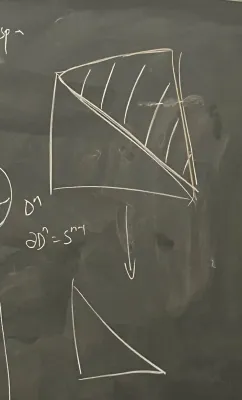
\includegraphics[width=0.25\textwidth]{Figures/simple_triangles.png}\]
\end{example}

\begin{definition}
    A homotopy equivalence $f: X \to Y$ between finite complexes is \textbf{simple} if it is homotopic to a sequence of collapses and expansions.
\end{definition}

Let us define the Whitehead torsion first, this is an obstruction to the homotopy equivalence being simple.
\begin{definition}
    For an acyclic (meaning the homologies are all zero) chain complex $(F_*, d)$ where each $F_n$ is free over $R$, the identity map $\operatorname{id}: F_* \to F_*$ is chain-homotopic to $0$. Thus, there exists some chain homotopy
    \[h: F_* \to F_{*+1} \text{ such that } dh + hd = id - 0 = id.\]
    From here, let $F_{even} = \bigoplus_{n \geq 0} F_{2n}$, and similarly $F_{odd}$, we define
    \[\tau(F_*, d) \coloneqq (F_{even} \xrightarrow{d + h} F_{odd}).\]
    We can check that $(d + h)(d + h) = id + h^2$, which is an isomorphism as the inverse is given by $id - h^2 + h^4 + ...$, so $d+h$ is an isomorphsm.\\

    In particular, for a homotopy equivalence $f: X \to Y$, this induces a lift $\Tilde{f}: \Tilde{X} \to \Tilde{Y}$ between their universal covers. The relative chain complex $C_*(\Tilde{Y}, \Tilde{X})$ is acyclic and $\Zbb[\pi_1]$-free. Thus, we define that
    \[\tau(f) \coloneqq \tau(C_*(\Tilde{Y}, \Tilde{X})) \in \operatorname{Wh}(\Zbb \pi_1(X)).\]
    Note that $\tau(f)$ is well-defined independent of the lift (the two different complexes differ by a deck transformation, which is modded out in the Whitehead group - as it is over $\pi_1(X)$).
\end{definition}

\begin{theorem}
For $f: X \to Y$ a homotopy equivalence between finite complexes, we can define the \textbf{Whitehead torsion} $\tau(f) \in \operatorname{Wh}(\pi_1 X)$ such that $\tau(f) = 0$ if and only if $f$ is simple.
\end{theorem}

\begin{proof}[Proof Idea]
    The idea is we can build $\operatorname{Wh}(G)$ is the set of equivalence classes of invertible matrices, where $A \in GL_m(R) \sim B \in GL_n(R)$ if $B$ can be obtained from $A$ by a sequence of following operations:
    \begin{enumerate}
        \item Elementary matrix operations.
        \item $A = \begin{pmatrix}
            B & 0\\
            0 & 1
        \end{pmatrix}$ or $B = \begin{pmatrix}
            A & 0\\
            0 & 1
        \end{pmatrix}$ (ie. collapse and expansions).
    \end{enumerate}
\end{proof}

\subsection{The s-cobordism Theorem}

\begin{definition}
    For smooth closed manifolds $M_0, M_1$. We say that $W$ is an \textbf{h-cobordism} between $M_0$ and $M_1$ if 
    \[\partial W = M_0 \sqcup M_1\]
    and the inclusion maps $M_0 \to W$ and $M_1 \to W$ are homotopy equivalences.
\end{definition}

\begin{example}
    $W = M_0 \times [0, 1]$ is the trivial $h$-cobordism.
\end{example}

\begin{definition}
    Let $M$ be a closed smooth manifold with dimension $\geq 5$, for an h-cobordism $W$ over $M$ (ie. $W$ is an h-cobordism between $M$ and some other manifold $M'$), we can define the \textbf{Whitehead torsion}
    \[\tau(W; M) \coloneqq \tau(M \hookleftarrow W) \in \operatorname{Wh}(\pi_1 M).\]
\end{definition}

\begin{theorem}[The s-cobordism Theorem]
Let $M$ be a closed smooth manifold with dimension $\geq 5$, for an h-cobordism $W$ over $M$, then
\begin{enumerate}
    \item $W$ is diffeomorphic to $M \times I$ if and only if $\tau(W; M) = 0$.
    \item The diffeomorphism classes of $h$-cobordisms over $M$ is in bijection with $\operatorname{Wh}(\pi_1 M)$, with the map given by the Whitehead torsion.
\end{enumerate}
\end{theorem}

\begin{proof}[Proof Idea]
    Using Morse theory, we can decompose every $h$-cobordism using handlebody decompositions. We can form a homology theory of handlebodies. The proof is similar to the case of Whitehead torsion in the last section. In this case, the elementary matrix operations correspond to handle slides, handle cancellations, and handle trading. We use a technique known as the \textbf{Whitney trick} to handle the collapse and expansion.
\end{proof}

\begin{remark}
    The letter $s$ in the s-cobordism theorem stands for the word ``simple".
\end{remark}

\begin{corollary}[The h-cobordism theorem]
    Every $h$-cobordism over simply-connected closed smooth $M$ of dimension $\geq 5$ is trivial.
\end{corollary}

As an application, we can prove the Poincare conjecture for dimension $\geq 6$.
\begin{theorem}
    For $n \geq 6$, if $M$ is a closed $n$-manifold homotopy equivalent to $S^n$, then $M$ is homeomorphic to $S^n$.
\end{theorem}

\begin{proof}
    Suppose $h: M \to S^n$ is a homotopy equivalence. Let $D_1^n, D_2^n$ be two disjoint disks on $M$. One can show that $W = M - \operatorname{int}(D_1 \cup D_2)$ is an $h$-cobordism between $\partial D_1^n$ and $\partial D^n_2$ (by computing some relative cohomology). By the h-cobordism theorem (here the dimension of the sphere is $\geq 5$), we have that
    \[W \cong \partial D_1^n \times [0, 1]. \]
    Thus, we have that $M$ is $\partial D_1^n \times [0,1]$ with $D_1^n$ and $D_2^n$ glued at the two ends, which shows $M$ is homeomorphic to $S^n$ (there is an Alexander's trick going on here).
\end{proof}

\newpage
\section{Lecture February 20th, 2025 - Athina Avrantini}

Today we will talk about Milnor K-theory \cite{MILNOR_k2}, which is an alternative, number theoretic, generalization of higher K-theory before Quillen's construction.

\subsection{Background on Quadratic Forms}

In this section, we fix $F$ to be a field whose characteristic is not $2$, and $V$ be a finite dimensional vector space over $F$.
\begin{definition}
    A quadratic form on a vector space $V$ is a map $q: V \to F$ such that
    \begin{enumerate}
        \item $q(\lambda x) = \lambda^2 q(x)$ for all $\lambda \in F$ and $x \in V$.
        \item The map $B_q: V \times V \to F$ given by $(x, y) \mapsto \frac{1}{2} [q(x+y)-q(x)-q(y)]$ is bilinear.
    \end{enumerate}
    We define the dimension of $q$ as the dimension of $V$.
\end{definition}

\begin{remark}
    Given a reasonable bilinear form $B_q: V \to F$, we can recover the information of a quadratic form by defining
    \[q(x) \coloneqq B_q(x, x).\]
\end{remark}

\begin{definition}
    We say a pair $(V, q)$ of a vector space and a quadratic form is \textbf{regular} (or \textbf{non-singular}) if for all $x \in V$, 
    \[B_q(x, y) = 0 \forall y \implies x = 0.\]
\end{definition}

\begin{definition}
    Two pairs $(V_1, q_1)$ and $(V_2, q_2)$ are \textbf{isometric} if there is an isomorphism of vector spaces $\phi: V_1 \to V_2$ such that
    \[q_2(\phi(x)) = q_1(x) \forall x \in V_1.\]
\end{definition}

From here we have our first proposition which we will not prove.
\begin{proposition}
    Every $n$-ary ($n$-variables) quadratic form is equivalent to some diagonal of the form
    \[d_1 x_1^2 + ... + d_n x_n^2\]
    by choosing an appropriate basis. In this case, we can rewrite the quadratic form as $\langle d_1, ...., d_n \rangle$.
\end{proposition}

\begin{definition}
    Given $(V_1, q_1)$ and $(V_2, q_2)$, we can form two operations
    \[(V_1 \oplus V_2, q_1 \oplus q_2), (q_1 \oplus q_2)(x_1, x_2) = q_1(x_1) + q_2(x_2).\]
    \[(V_1 \otimes_F V_2, q_1 \otimes q_2), (q_1 \otimes q_2)(x_1 \otimes x_2) = q_1(x_1) q_2(x_2).\]
\end{definition}

\begin{definition}
    We say the pair $(V, q)$ is \textbf{isotropic} if there exists $x \in V \setminus \{0\}$ such that $q(x) = 0$. Otherwise, we say that $(V, q)$ is \textbf{anisotropic}.
\end{definition}

\begin{proposition}
    If $(V, q)$ is two dimensional, then the following are equivalent.
    \begin{enumerate}
        \item $(V, q)$ is regular and isotropic.
        \item $(V, q) = (F^2, (x, y) \mapsto xy) \cong (F^2, (x, y) \mapsto x^2 - y^2)$. Note the functions here are bilinear forms, and you take their correspondent quadratic forms (which has signature $+1, -1$).
    \end{enumerate}
    The isometry class satisfying any of these two conditions is called the \textbf{hyperbolic plane}, denoted by $\mathcal{H}$.
\end{proposition}

\begin{definition}
An orthogonal sum of $\mathcal{H}$ is called a \textbf{hyperbolic spaces}. The corresponding quadratic form on a hyperbolic space is of the form
    \[(x_1^2 - x_2^2) + ... + (x^2_{2m-1} + x^2_{2m}) \text{ or equivalently } x_1 x_2 + ... + x_{2m-1} x_{2m}.\]
\end{definition}

\subsection{Grothendieck-Witt Rings}

Let $M(F)$ be the isometry classes of \textbf{regular quadratic forms} over $F$. Note that $\oplus, \otimes$ gives $M(F)$ the structure of a \textbf{semi-ring}. In fact, $M(F)$ also satisfies additive cancellation (ie. $q \oplus q_1 \cong q \oplus q_2$ implies $q_1 \cong q_2$.)

\begin{definition}
    We define the \textbf{Grothendieck-Witt ring} of $F$ as
    \[\hat{W}(F) \coloneqq \text{Grothendieck group completion of } M(F).\]
    Note that, as before, every element in $\hat{W}(F)$ has the form $q_1 - q_2$ (formal difference of two quaratic forms).
\end{definition}

By the universal property of Grothendieck group completion, the map $\dim: M(F) \to \Zbb$ induces a a well-defined map
\[\dim: \hat{W}(F) \to \Zbb \text{ with } \dim(q_1 - q_2) = \dim q_1 - \dim q_2.\]

\begin{definition}
    We define $\hat{I} F \coloneqq \ker(\dim)$ as the \textbf{augmentation ideal}. 
\end{definition}

\begin{proposition}
    The subgroup generated by the hyperbolic plane $\mathcal{H}$ in $\hat{W}(F)$ is an ideal. Intuitively, this is the ideal consisting of all hyperbolic spaces an their inverses.
\end{proposition}

\begin{proof}[Proof Idea]
   Additive closure is clear. For scalars, show that for a quadratic form $q$, $q \otimes \mathbb{H} \cong \bigoplus_{i = 1}^{\dim q} \mathcal{H}$.
\end{proof}

\begin{definition}
    The \textbf{Witt ring} of $F$ is defined as
    \[W(F) \coloneqq \hat{W}(F)/ \langle \mathcal{H} \rangle.\]
    We let $IF$ be the image of $\hat{I} F$ in $W(F)$. $IF$ is called the \textbf{fundamental ideal} of $W(F)$.
\end{definition}

\begin{remark}
The elements of $W(F)$ are in bijection with the isometry classes of anisotropic forms.    
\end{remark}

The modern theory of quadratic forms are interested in a filtration given by
\[W(F) \supset IF \supset I^2 F \supset I^3 F \supset ... \text{ and the factors } I^n F/I^{n+1} F,\]
which we will see more later in this talk.

\begin{proposition}
    $W(F)/IF \cong \Zbb/2\Zbb$. Colloquially, we can think of the fundamental ideal $IF$ as comprising of all forms of even dimensions.
\end{proposition}

\subsection{Central Simple Algebra and Brauer Group}

\begin{definition}
    A finite dimensional $F$-algebra $A$ is a \textbf{central simple algebra (CSA)} if 
    \begin{itemize}
        \item It is simple (ie. has no non-trivial two sided ideals)
        \item The center of $A$ is $F$.
    \end{itemize}
\end{definition}

\begin{definition}
    The \textbf{Brauer group} of $F$ is given by
    \[\operatorname{Br}(F) = \{\text{CSAs over $F$}\}/\sim\]
    where we say $A \sim B$ if there exists finite dimensional vector spaces $V$ and $W$ such that we have the following isomorphism of $F$-algebras:
    \[A \otimes_F \operatorname{End}(V) \cong B \otimes_F \operatorname{End}(W).\]
    The group operation on the Brauer group is given by the tensor product. The inverses are given by the opposite algebra (ie. $[A]^{-1} = [A^{op}]$). The identity is given by $[F]$. The group operation is commutative, so the Brauer group is abelian.
\end{definition}

\begin{definition}
    For $a, b \in F^{\times}$, the \textbf{quarternion algebra} $(\frac{a, b}{F})$ is the \textbf{central simple algebra} generated by $\{i, j\}$ with the relations:
    \begin{itemize}
        \item $i^2 = a$
        \item $j^2 = b$
        \item $ij = -ji$.
    \end{itemize}
\end{definition}

\begin{lemma}
    The element $(\frac{a, b}{F})$ has order 2 in $\operatorname{Br}(F)$.
\end{lemma}

\begin{proof}
    Given a quarternion algebra $(\frac{a, b}{F})$, there is a conjugation operation $\operatorname{conj}: (\frac{a, b}{F}) \to (\frac{a, b}{F})$ such that
    \[\operatorname{conj}(a + ib + jc + (ij) d) = a - ib - jc - ij d.\]
    (sometimes, we use the overline notation to indicate the conjugation). Notably, the conjugation map described here is actually not multiplicative, but rather anti-multiplicative, in the sense that
    \[\operatorname{conj}(x y) = \operatorname{conj}(y) \operatorname{conj}(x).\]
    This corresponds to a multiplicative map $(\frac{a,b}{F}) \to (\frac{a, b}{F})^{op}$. In particular, this conjugation map yields as an isomorphism
    \[(\frac{a,b}{F}) \cong (\frac{a, b}{F})^{op}.\]
    Equivalently, this means that the element is its own inverse in the Brauer group.
\end{proof}

\begin{example}
    When $F = \Rbb$ and $a, b = -1$, we have that the ordinary qurternion $\mathbb{H}$ is given by
    \[\mathbb{H} \cong (\frac{a, b}{F}).\]
    Since conjugation gives an isomorphism to the opposite algebra, we have that $\mathbb{H}$ has order two in $Br(\Rbb)$. In fact, $Br(\Rbb) = \Zbb/2\Zbb$.
\end{example}

\begin{definition}
    Given a quarternion algebra $(\frac{a, b}{F})$, the norm map is given by $N(x) \coloneqq x \overline{x}$ for $x \in F$. One can check that the norm map is a quadratic form on $(\frac{a, b}{F})$. In terms of the orthogonal basis $1, i, j, ij$, this quadratic form can be represented by the coefficients $\langle 1, -a, -b, ab \rangle \cong \langle 1, - a \rangle \otimes \langle 1, -b \rangle$.
\end{definition}

% \textbf{Fact:} For quarternion algebras. $\operatorname{Norm}(x) \coloneqq x \cdot \overline{x}$ corresponds to a quadratic form on $(\frac{a, b}{F})$.\\

\subsection{Going to K-Theory $K_2(F)$}

Recall that for a field $F$, we have that
\[K_0(F) = \Zbb \text{ and } K_1(F) = F^{\times}.\]

\begin{definition}
   For $n = 0, 1$, we define $k_n(F) \coloneqq K_n(F) / 2K_n(F)$. In this case we see that
   \[k_0(F) = \Zbb/2\Zbb \cong W(F)/IF \text{ and } k_1(F) = F^{\times} /2F \cong IF/I^2F.\]
   Here $k_0(F)$ should be thought of as dimension mod 2 and $k_1(F)$ should be thought of as ``signed determinant".
\end{definition}

\begin{remark}
    Let $d(q)$ be the assoicated determinant and $n = \dim q$. Observe that $q$ lies in $I^2 F$ if $n$ is even and either
    \begin{itemize}
        \item $d(q) = 1$ and $4$ divides n
        \item Or, $d(q) = -1$ and $4$ does not divide $n$.
    \end{itemize}
\end{remark}

The idea Milnor had was to define an appropriate definition of $K_2(F)$ such that its associated $k_2(F)$ satisfies
\[k_2(F) \cong I^2 F/ I^3 F.\]

We can attempt to generalize this with the aid of the following definition.
\begin{definition}
    Let $G$ be abelian, a pairing
    \[[\bullet, \bullet]: F^{\times} \times F^{\times} \to G\]
    is a \textbf{Steinberg symbol} if it is (bi)multiplicative and it satisfies what is called the \textbf{Steinberg relations}, that is
    \[a + b = 1 \implies [a, b] = 1.\]
    (Here the symbol has the data of a map and a group $G$).
\end{definition}

\begin{definition}[``Milnor's" $K_2$ of $F$]
    We define $K_2(F) = F^\times \otimes_{\Zbb} F^\times / \langle a \otimes b: a + b = 1 \rangle$. We also let $k_2(F) \coloneqq K_2(F)/2K_2(F)$.
\end{definition}

\begin{remark}
    This is not the original definition Milnor gave in his 1968 paper. However, by a theorem of Matsumoto, this is equivalent to Milnor's original definition. The definition presented here was given in a 1970 paper.
\end{remark}

There is a natural map $F^{\times} \otimes_{\Zbb} F^{\times} \to K_2(F)$ by passing through the quotient. There is another natural map $F^{\times} \otimes_{\Zbb} F^{\times} \to k_2(F) = K_2(F)/2K_2(F)$ by composing the previous map by another quotient map. With an abuse of notation, we will use $[a, b]$ to denote the image of $a \otimes b$ in both $K_2(F)$ and $k_2(F)$.\\

By construction we observe that $K_2(F)$ has the universal property.
\begin{proposition}
$K_2(F)$ has the following universal property. For any $f: F^{\times} \times F^{\times} \to G$, there exists a unique group homomorphism $g: K_2(F) \to G$ such that the following diagram commutes
% https://q.uiver.app/#q=WzAsMyxbMCwwLCJGXntcXHRpbWVzfSBcXHRpbWVzIEZee1xcdGltZXN9Il0sWzEsMCwiS18yKEYpIl0sWzAsMSwiRyJdLFswLDIsImYiLDJdLFswLDEsIlxcdGV4dHtuYXR1cmFsIHF1b3RpZW50fSJdLFsxLDIsIlxcZXhpc3RzICEgZywgXFx0ZXh0eyBncm91cCBob20gfSJdXQ==
\[\begin{tikzcd}
	{F^{\times} \times F^{\times}} & {K_2(F)} \\
	G
	\arrow["{(a,b) \mapsto [a,b]}", from=1-1, to=1-2]
	\arrow["f"', from=1-1, to=2-1]
	\arrow["{\exists ! g, \text{ group hom }}", from=1-2, to=2-1]
\end{tikzcd}\]
\end{proposition}

 We observe that $k_2(F) \coloneqq K_2(F)/2K_2(F)$ similarly has the following property. The takeaway is that the map $(a, b) \mapsto [a, b] \in k_2(F)$ can be thought of as the ``mod 2 universal Steinberg symbol". 
\begin{proposition}
    Similarly, $k_2(F)$ has the following universal property for all $G$ with $x^2 = 1$ for all $x \in G$ (such $G$ is called a 2-torsion group). For all group homomorphisms $f: F^{\times} \times F^{\times} \to G$, there exists a unique group homomorphism $g: k_2(F) \to G$ such that the following diagram commutes:
\[\begin{tikzcd}
	{F^{\times} \times F^{\times}} & {k_2(F)} \\
	G
	\arrow["{(a, b) \mapsto [a, b]}", from=1-1, to=1-2]
	\arrow["f"', from=1-1, to=2-1]
	\arrow["{\exists ! g, \text{ group hom }}", from=1-2, to=2-1]
\end{tikzcd}\]
\end{proposition}

We state the following proposition where most of the proofs are explained in the passage.
\begin{proposition}
    \begin{enumerate}
        \item Let $_2 Br(F) \coloneqq \{x \in Br(F)\ |\ x^2 = 1\}$ be the subgroup of two torsion elements, then the map
        \[(a, b) \mapsto (\frac{a, b}{F}) \in _2 Br(F) \]
        is a Steinberg symbol, so there exists an unique group homomorphism
        \[\beta: k_2(F) \to {_2Br(F)}, [a, b] \mapsto (\frac{a, b}{F})\]

        \item The map $F^{\times} \times F^{\times} \to I^2 F/ I^3 F$ given by
        $$(a, b) \mapsto \langle 1, -a \rangle \otimes \langle 1, -b \rangle \mod I^3 F$$ is a Steinberg symbol. Thus, we get a unique group homomorphism
        \[\alpha: K_2(F) \to I^2 F/ I^3 F\]

        \item We have produced maps
        % https://q.uiver.app/#q=WzAsMyxbMSwwLCJrXzIoRikiXSxbMCwxLCJJXjIgRi9JXjMgRiJdLFsyLDEsIl8yIEJyKEYpIl0sWzAsMiwiXFxiZXRhIl0sWzAsMSwiXFxhbHBoYSIsMl0sWzEsMiwiXFxleGlzdHMgXFxnYW1tYSIsMix7InN0eWxlIjp7ImJvZHkiOnsibmFtZSI6ImRhc2hlZCJ9fX1dXQ==
\[\begin{tikzcd}
	& {k_2(F)} \\
	{I^2 F/I^3 F} && {_2 Br(F)}
	\arrow["\alpha"', from=1-2, to=2-1]
	\arrow["\beta", from=1-2, to=2-3]
	\arrow["{\exists \gamma}"', dashed, from=2-1, to=2-3]
\end{tikzcd}\]
From well known facts in quadratic forms, there exists a map $\gamma: I^2 F/ I^3 F \to _2 Br(F)$ induced by what is called the \textbf{Clifford invariant}, such that the diagram above commutes.
    \end{enumerate}
\end{proposition}

\begin{theorem}[Milnor, 1970]
    The map $\alpha$ is an isomorphism.
\end{theorem}

The proof of Milnor's result invovled the use of Stiefel-Whitney invariants.

\begin{theorem}[Merkurjev, 1981]
   The map $\gamma$ is an isomorphism.
\end{theorem}

Thus, as a corollary, we have that
\begin{theorem}
    $\beta: k_2(F) \to {_2 Br(F)}$ is an isomorphism.
\end{theorem}

\begin{remark}
    The three maps being isomorphisms unifies three seemingly unrelated objects:
    \begin{enumerate}
        \item $k_2(F)$ is a group derived from the K-theory of fields.
        \item $I^2F/I^3 F$ is a group from quadratic form theory.
        \item $_2 Br(F)$ is a group associated to central simple algebras with $F$-involution.
    \end{enumerate}
\end{remark}

\begin{proposition}
    Let $\Fbb_q$ be a finite field of order prime power $q$. $K_2(\Fbb_q) = 0$.
\end{proposition}

\begin{proof}[Proof Sketch]
    $\Fbb_q^{\times}$ is cyclic and thus has generator $a$. Note that an element in $K_2(\Fbb_q)$ is always of the form $[a^m, a^n]$. From here,  we have that
    \[[a^m , a^n] = [a, a]^{mn} = [a, -1]^{mn}.\]
    A fun exercise is to show that $[a, -1]$ has order $\leq 2$ in $K_2$. This implies that $K_2(F)$ is cyclic of order $\leq 2$.\\
    
    On the other hand, we can show that there exists odd $r$ such that $[a, a]^r = 1$. If this is the case, we can conclude that $K_2(F) = 0$. Indeed, we can find a non-square element $b \in F^{\times}$ (the existence of such element really comes from finite field theory). For $b$, there exists non-zero elements $x, y$ such that $v x^2 + by^2 = 1$. Since $\Fbb_q^{\times}$ is cyclic, we can write
    \[bx^2 = a^s \text{ and } by^2 = a^t.\]
    Since $b$ is not a square, $s$ and $t$ cannot be even. On the other hand, we see that
    \[[a, a]^{st} = [a^s, a^t] = [bx^2, by^2] = 1,\]
    where the last equality follows from the Steinberg relations.
\end{proof}

\subsection{Milnor's Higher K-Groups}

We first introduce a notation of Milnor that converts the multiplicative structure to an additive structure.
\begin{definition}
    View $K_1(F)$ as the additive version of $F^{\times}$, there is a canonical isomorphism $\ell: F^{\times} \to K_1(F)$ with
    \[\ell(ab) = \ell(a) + \ell(b).\]
\end{definition}

\begin{definition}
    Define $K_*(F)$ as the quotient of the tensor algebra $T(K_1(F))$ (with base $\Zbb$) by the ideal generated by elements of the form 
    \[\ell(a) \otimes \ell(1 - a), \forall a \in F \setminus \{0, 1\}.\]
    Concretely, $K_n(F)$ is given by
    \[K_n(F) \coloneqq \frac{\bigotimes_{i=1}^n K_1(F)}{\langle \ell(a_1) \otimes ... \otimes \ell(a_n) | a_i + a_{i+1} = 1 \text{ for some $i < n$}, a_i \in F \setminus \{0, 1\} \rangle}\]
    Hence forward, we can identify $[a, b]$ with $\ell(a) \otimes \ell(b)$.
\end{definition}

\begin{remark}
    We recover the definition for $K_2(F)$ by identifying $\ell(a) \otimes \ell(b)$ with $[a, b]$.
\end{remark}

\begin{proposition}
    For $n > 2$, $K_n(F)$ is generated by $K_2(F) \cdot K_{n-2}(F)$. Note that this implies that $K_n(\Fbb_q) = 0$ for a finite field $\Fbb_q$.
\end{proposition}

This computation shows that Milnor's Higher K-theory are different from what eventually became the definition for Quillen's Algebraic K-theory. When $n \leq 2$, the two notions do agree, though.

\begin{definition}
Generalizing the Steinberg symbol, we can define the $n$-fold Steinberg symbol
\[(a_1, ..., a_n) \mapsto \langle 1, a_1 \rangle \otimes ... \otimes \langle 1, a_n \rangle \mod I^{n+1} F.\]
\end{definition}

\textbf{Fun Fact:} Form of the finite on the RHS are called \textbf{Pfister forms}.\\

In this case, we similarly have universal properties, which similarly gives us unique homomorphism taking $\ell(a_1) \otimes ... \ell(a_n)$ to the RHS. Furthermore, $I^{n}F/I^{n+1}F$ is an elementary 2-group.
\begin{proposition}
    There is a well-defined unique homomorphism $\alpha_n: k_n(F) \to I^{n} F/ I^{n+1} F$ taking
    \[\ell(a_1) \otimes ... \ell(a_n) \mapsto \langle 1, a_1 \rangle \otimes ... \otimes \langle 1, a_n \rangle \mod I^{n+1} F.\]
\end{proposition}

\begin{question}
When $n \leq 2$, $\alpha_n$ is an isomorphism. What about $n > 2$?    
\end{question}

\begin{conjecture}[Milnor's First Conjecture]
    $\alpha_n$ is an isomorphism for all $n$ and for all fields $F$.
\end{conjecture}

We can also define $\beta_n: k_n(F) \to H^n(F, \Zbb/2)$ (which when $n = 2$, gives the elements of order 2 in the Brauer group). Here $H^n(F, \Zbb/2)$ is the Galois cohomology with $\Zbb/2$-coefficients.
\begin{conjecture}[Milnor's Second Conjecture]
  $\beta_n: k_n(F) \to H^n(F, \Zbb_2)$ is also an isomorphism.  
\end{conjecture}

The first conjecture was proven by Orlov, Vishik, and Voevodsky in the 1990s. The second conjecture was proven by Voevodsky in 2002, which awarded him the fields medal. The proof of these two theorems involved the machineries of \textbf{motivic cohomology} \cite{Voevodsky2003}.

\newpage
\section{Lecture February 25th, 2025 - Mattie Ji}\label{sec::plus_construction}

In this note, we will discuss Quillen's Plus construction for defining higher algebraic K-theory and compute the algebraic K-theories of finite fields \cite{quillen_plus}. Some other very helpful references for preparing the lectures were \cite{MitchellKtheoryFinFields, EgasSantander2010, Haine_KtheoryFiniteFields, peroux_ktheory, NiemiroZhang2022}. This presentation, however, is very much a historical revisionist approach.

\subsection{Quillen's Plus Construction}

Before going into Quillen's Plus construction, let us first recall the following constructions from MATH 6180.
\begin{theorem}\label{thm::principal_G}
    Let $G$ be a topological group, there exists a principal $G$-bundle\footnote{It's okay if you have never seen the word before, just think about this theorem as an existence statement for a pair of nice spaces.} $EG \to BG$ such that:
    \begin{enumerate}
        \item $G \to EG \to BG$ is a fibration and $EG$ is contractible.
        \item If $G$ is discrete, then $BG = K(G, 1)$.
        \item $EG \to BG$ is ``the universal principal $G$-bundle".
    \end{enumerate}
\end{theorem}

\begin{definition}
    Let $f: X \to Y$ be a map (not necessarily a fibration). Consider the pullback of the diagram
    % https://q.uiver.app/#q=WzAsNCxbMCwwLCJFX2YiXSxbMSwwLCJZXkkiXSxbMSwxLCJZIl0sWzAsMSwiWCJdLFszLDIsImYiLDJdLFsxLDIsIlxcZ2FtbWEgXFxtYXBzdG8gXFxnYW1tYSgwKSJdLFswLDFdLFswLDNdXQ==
\[\begin{tikzcd}
	{E_f} & {Y^I} \\
	X & Y
	\arrow[from=1-1, to=1-2]
	\arrow[from=1-1, to=2-1]
	\arrow["{\gamma \mapsto \gamma(0)}", from=1-2, to=2-2]
	\arrow["f"', from=2-1, to=2-2]
\end{tikzcd}\]
    The map $E_f \to Y$ given by $(x, \gamma) \mapsto \gamma(1)$ is a fibration, we let the \textbf{homotopy fiber} of $f$, $\operatorname{Hofib}(f)$, be the fiber of $E_f \to Y$.
\end{definition}

Let $f: X \to Y$ be a map, the homotopy fiber yields a long exact sequence of homotopy groups reminisicient of that of the long exact sequence from a fibration:
\[... \to \pi_{n+1}(Y) \to \pi_n(\operatorname{HoFib}(f)) \to \pi_n(X) \to \pi_n(Y) \to ...\]

\begin{definition}
    A space $X$ is \textbf{acyclic} if $\Tilde{H}_*(X; \Zbb) = 0$. A map $f: X \to Y$ is \textbf{acyclic} if $\operatorname{Hofib}(f)$ is acyclic.
\end{definition}

\begin{lemma}
    An acyclic map $f: X \to Y$ induces an equivalence of $\Zbb$-homologies.
\end{lemma}

\begin{proof}
  Recall that for a fibration $\operatorname{HoFib}(f) \to E_f \simeq X \to Y$, if $\pi_1(Y)$ acts trivially on $H_*(\operatorname{HoFib}(f))$, then we have a Serre spectral sequence. Indeed, $\operatorname{HoFib}(f)$ is acyclic, so the action is trivial and hence we have a spectral sequence given by
  \[E^2_{p, q} = H_p(Y; H_q(\operatorname{HoFib}(f); \Zbb)) \implies H_{p+q}(X; \Zbb).\]
  On the other hand, $E^2_{p, q} = 0$ for all $q \neq 0$, so the spectral sequence collapses on the $E_2$-page. Thus, we have an isomorphism given by
  \[H_p(Y; \Zbb) \cong H_p(X; \Zbb).\]
\end{proof}
In fact, with a bit more argument, one can show that an acyclic map $f: X \to Y$ induces an equivalence between any local coefficient systems, and the converse is also true.\\

The acyclic map aids us in creating what is called the plus construction.
\begin{definition}
    A group $G$ is called perfect if $G = [G, G]$. For a pointed connected complex $X$, let $N \triangleleft \pi_1(X)$ be a perfect normal subgroup. A \textbf{plus construction of $X$ relative to $N$} is a pair $(X, i: X \to X^+)$ such that $i$ is acyclic and $N = \ker(i_*: \pi_1(X) \to \pi_1(X^+))$. (Note that such maps have to be surjective on $\pi_1$ as well)
\end{definition}

Last semester in MATH 6180, we showed that such plus construction always exists (albeit we only proved the map induces an isomorphism of integral homologies, rather than being acyclic, but our construction does induce an isomorphism over all local coefficient systems and hence gives an acyclic map) and satisfy a universal property.

\begin{theorem}
 Let $X$ be as above and $N$ be a perfect normal subgroup of $\pi_1(X)$.
 \begin{enumerate}
     \item There exists a plus construction $i: X \to X^+$ of $X$ relative to $N$.
     \item Let $f: X \to Y$ be a map such that $N \subseteq \ker(f_*)$, then there exists a map $f^+: X^+ \to Y$, unique up to based homotopy, such that the following diagram commutes up to based homotopy:
     % https://q.uiver.app/#q=WzAsMyxbMCwwLCJYIl0sWzEsMCwiWF4rIl0sWzEsMSwiWSJdLFswLDEsImkiXSxbMSwyLCJmXisiXSxbMCwyLCJmIiwyXV0=
\[\begin{tikzcd}
	X & {X^+} \\
	& Y
	\arrow["i", from=1-1, to=1-2]
	\arrow["f"', from=1-1, to=2-2]
	\arrow["{f^+}", from=1-2, to=2-2]
\end{tikzcd}\]
 \end{enumerate}
\end{theorem}

The connection from the plus construction to algebraic K-theory is given by the following lemma.
\begin{lemma}
    Let $R$ be a ring, then $[\GL(R), \GL(R)]$ is a perfect normal subgroup of $\GL(R)$.
\end{lemma}

\begin{proof}
    Clearly the commutator subgroup is normal and recall that $E(R) = [\GL(R), \GL(R)]$. To show that $E(R)$ is perfect, we use the following lemma of Whitehead without proof.
    \begin{lemma}
        For $i, j, k$ all distinct, $e_{ij}(x) = [e_{ik}(x), e_{kj}(1)]$.
    \end{lemma}
    Thus, it follows from the lemma that for $n \geq 3$, $E_n(R)$ is perfect. Since $E(R)$ is the colimit of $E_n(R)$ for $n \geq 3$, and a colimit of perfect groups is perfect, we have that $E(R)$ is perfect.
\end{proof}

From here, we define the higher algebraic K-theory as follows.
\begin{definition}
    Let $R$ be a ring, observe that $\pi_1(\operatorname{BGL}(R)) = GL(R)$. Let $\operatorname{BGL}(R)^+$ denote the plus construction with respect to the perfect normal subgroup $[\GL(R), \GL(R)]$. For $i > 1$, we define
    \[K_i(R) \coloneqq \pi_i(\operatorname{BGL}(R)^+).\]
    Here, $K_0$ is defined separately as before and note that the definition agrees with $K_1$ and $K_2$.\\

    For convenience, we also write $K(R) \coloneqq K_0(R) \times \operatorname{BGL}(R)^+$. In this case we have that $K_i(R) = \pi_i(K(R))$ for all $i \geq 0$.
\end{definition}

\begin{remark}
    Let $R = \Rbb$ or $\Cbb$ be the standard Euclidean topological fields (as opposed to discrete topology),  then the plus construction recovers real topological K-theory and complex topological K-theory respectively.
\end{remark}

\begin{remark}
    The following is an alternative construction of the higher algebraic K-theories. This is certainly dated before my source, but I saw this from a post by Tom Goodwillie.\\

    Once again $K_0$ is defined separately. For $n > 1$, we inductively define $K_n(R)$ as follows.
    \begin{enumerate}
        \item We define $K_1(R) \coloneqq H_1(\operatorname{BGL}(R))$. The natural map $\operatorname{GL}(R) \to K_1(R)$ induces a map $\phi_1: \operatorname{BGL}(R) \to BK_1(R)$. Let $F_1$ be the homotopy fiber of $\phi_1$.
        \item Suppose $F_{n-1}$ has been defined, we define $K_n(R) \coloneqq H_n(F_{n-1})$. There is an induced map from $\phi_n: F_{n-1} \to B^n K_n(R)$ that represents identity on $H_n$, and we let $F_n$ be the homotopy fiber of $\phi_n$.
    \end{enumerate}
\end{remark}

Let us examine some properties of $\operatorname{BGL}(R)^+$ first.\\

For $n > 1$, recall that for a path $\gamma: [0, 1] \to X$, $\gamma$ induces an isomorphism $\beta_{\gamma}: \pi_n(X, \gamma(0)) \to \pi_n(X, \gamma(1))$ given by sending $[f: (I^n, \partial I^n) \to (X, \gamma(0))]$ to a map $[\gamma f: (I^n, \partial I^n) \to (X, \gamma(1))$ of the form
\[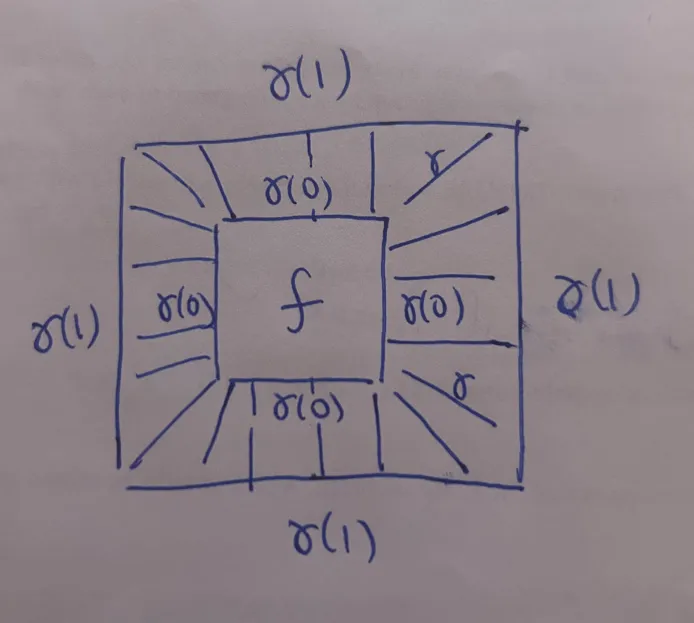
\includegraphics[width=0.3\textwidth]{Figures/path_act_pin.png}\]
For a loop $\gamma \in \pi_1(X, \gamma(0))$, $\beta_{\gamma}$ naturally arises as an element of $\operatorname{Aut}(\pi_n(X, \gamma(0)))$ and thus this gives a group action of $\pi_1(X, \gamma(0))$ on $\pi_n(X, \gamma(0))$. When $n = 1$, we define the group action by conjugation.

\begin{definition}
    A connected space $X$ is \textbf{simple} if it has abelian fundamental group and the action of $\pi_1$ on $\pi_n$ is trivial for $n > 1$.
\end{definition}

\begin{example}
    Any connected H-space is simple. In particular, $\operatorname{BGL}(R)^+$ is simple since it has an H-space structure. A careful proof can be found in Wagoner's \textit{Delooping Classifying Spaces in Algebraic K-Theory} (1971).
\end{example}

The following is a generalization of the fact that a map inducing isomorphism of $\Zbb$-homologies between simply connected spaces is a weak homotopy equivalence.
\begin{proposition}\label{prop::weak_hom_equiv_simple}
    Let $\phi: X \to Y$ be a map of simple connected CW complexes such that $\phi_*$ is an isomorphism on $\Zbb$-homologies. Then $\phi$ is a homotopy equivalence.
\end{proposition}

\begin{remark}
This definition for higher algebraic K-theory may seem somewhat random. Its ability to recover topological K-theories is one motivation. As far as the writer knows, another central motivation came from a key step in Quillen's proof of the \textbf{Adams conjecture}.\\

Roughly speaking, the \textbf{Adams conjecture} is a statement about the images of J-homomorphisms of differences of a bundle with its image under the Adams operations $\psi^q$. A key step of Quillen's proof was showing that there is a $\Zbb$-homology equivalence from $\operatorname{BGL}(\Fbb_q)$ to $F\psi^q$ (this will be defined later). This is not a homotopy equivalence, but the induced map from the plus construction would be a homotopy equivalence by the previous proposition.\\

Allegedly, Dennis Sullivan introduced the idea of the plus construction to Quillen. The plus constructions themselves were introduced earlier by Kervaire to construct homology spheres.
\end{remark}

\subsection{Outline for the K-Theory of Finite Fields}
From now on we fix $\Fbb_q$ be a finite field of $q = p^n$ elements (for $p$ prime).
\begin{theorem}
    For $i > 0$, we have that
    $$K_{2i}(\Fbb_q) = 0 \text{ and } K_{2i-1}(\Fbb_q) = \Zbb/(q^n - 1)\Zbb.$$
\end{theorem}

% \begin{corollary}
%    For $i > 0$, we have that
%     $$K_{2i}(\overline{\Fbb_p}) = 0 \text{ and } K_{2i-1}(\overline{\Fbb_p}) = \bigoplus_{\ell \neq p \text{ prime}} \Qbb_\ell/\Zbb_\ell.$$ 
% \end{corollary}

Before we compute the K-theory of finite fields, we first describe the general outline of how this is proven.
\begin{definition}
    For general space $X$ (not necessarily compact or Hausdorff), we define
    \[\KU^0(X) \coloneqq [X, BU \times \Zbb] \text{ and } \KU^1(X) \coloneqq [X, \Omega BU].\]
\end{definition}

\begin{enumerate}
    \item Let $\psi^q$ be the Adams operations. There is a way to extend the \textbf{Adams operations} $\psi^q$ onto $\KUr^0(BU) \to \KUr^0(BU)$. From here we can actually produce a map $\psi^q - 1: BU \to BU$ whose induced map on complex K-theory is $\psi^q - 1$.

    \item Let $F\psi^q$ be the homotopy fiber of $\psi^q - 1$, then the homotopy groups of $F\psi^q$ are quite computable by the long exact sequence - those are exactly what is given in the theorem. Furthermore, $F\psi^q$ is simple.
    
    \item The idea is that we can construct a map $\theta: \BGL(\Fbb_q) \to F\psi^q$ that is an equivalence of $\Zbb$-homologies. By the universal property, this induces a map $\theta^+: \BGL(\Fbb_q)^+ \to F\psi^q$ that is a $\Zbb$-homology equivalence between simple spaces and is thus a homotopy equivalence by Prposition~\ref{prop::weak_hom_equiv_simple}.

    \item The construction of the map $\theta: \BGL(\Fbb_q) \to F\psi^q$ is done using representation theory and what is called a \textbf{Brauer lift}.
\end{enumerate}


\subsection{The Adams Operations on $BU$ and $F\psi^q$}

Recall we have previously defined the Adams operations as follows.

\begin{theorem}[Adams' Operations Theorem]\label{thm::adams_operations}
    There exist ring homomorphisms $\psi^k: \KU^0(X) \to \KU^0(X)$ defined on all compact Hausdorff spaces $X$ such that:
    \begin{enumerate}
        \item (Naturality): For $f: X \to Y$, we have $\psi^k f^* = f^* \psi^k$.
        \item If $L \to X$ is a line bundle, then $\psi^k(L) = L^k$.
        \item $\psi^{k} \circ \psi^{\ell} = \psi^{k \ell}$.
        \item When $p$ is prime, for each $\alpha$, there exists some $\beta \in \KU^0(X)$ such that $\psi^p(\alpha) = \alpha^p + p \beta$. We think of this as $\psi^p(\alpha) \equiv \alpha^p \mod p$.
        \item By naturality, $\psi^k$ restricts to a map $\KUr^0(X) \to \KUr^0(X)$. When $X = S^{2n}$, $\psi^k$ acts as multiplication by $k^{n}$ on $\KUr^0(X)$.
    \end{enumerate}
\end{theorem}

The naive idea of constructing $\psi^q$ on the level of $BU$ is as follows. Suppose we have defined $\psi^q: \KUr^0(BU) \to \KUr^0(BU)$. Then the Adams operations is a natural transformation from $[BU, BU] \to [BU, BU]$, a Yoneda lemma type argument then shows that there exists a map $\psi^q: BU \to BU$ lifting the level on complex K-theory.\\

However, we have not established the Adams' operations on $BU$ yet. To do this, we need to introduce the following algebraic tool.
\begin{definition}
    Let $... \to A_3 \xrightarrow{f_2} A_2 \xrightarrow{f_1} A_1 \xrightarrow{f_0} A_0$ be a sequence of abelian groups. Define a map
    \[\partial: \prod_{n} A_n \to \prod_{n} A_n, (a_n)_{n \geq 0} \mapsto (a_n - f_n(a_{n+1}))_{n \geq 0}.\]
    We define $\lim_{\leftarrow n}^1 A_n$ as the cokernel of $\partial$.
\end{definition}

\begin{theorem}[Milnor Exact Sequence]
Write $X = \lim_{\to n} X_n$ be a pointed CW-complex, and let $\Tilde{E}^{\bullet}$ be a (reduced, additive) generalized cohomology theory, then there is a short exact sequence
\[0 \to \lim_{\leftarrow n}^1 \Tilde{E}^{\bullet - 1}(X_n) \to \Tilde{E}^{\bullet}(X) \to \lim_{\leftarrow n} \Tilde{E}^{\bullet}(X_n) \to 0.\]
\end{theorem}

It turns out that one can build a cell complex structure of $BU$ as $\bigcup_{n = 1}^\infty X_n$ that only has even dimensional cells. Applying the Milnor exact sequence for complex K-theory and $\bullet = 0$ gives us
\[0 \to \lim_{\leftarrow n}^1 \KUr^{-1}(X_n) \to \KUr^0(BU) \to \lim_{\leftarrow n}^1 \KUr^0(X^n) \to 0 \]
On the other hand, by Bott periodicity and the long exact sequence (you could even use the 3-term one) of pairs for $(X_{2m+2}, X_{2m})$, we have that $\KUr^{-1}(X_n) = 0$ for all $n$. Thus, we have that
\[\KUr^0(BU) = \lim_{\leftarrow n} ^1 \KUr^0(X^n).\]

\begin{definition}
Since the $\psi^q$'s are well-defined on $\KUr^0(X^n)$, we can extend them to $\KUr^0(BU)$ via this isomorphism. Thus, we have obtained well-defined maps $\psi^q: BU \to BU$.    
\end{definition}

Now $\operatorname{BU}$ itself has the structure of a (homotopy associative and commutative) $H$-space (by Bott periodicity) and hence there is a well-defined $H$-space structure $m: BU \times BU \to BU$. The natural transformation represented by $-1$ can also be realized as a map $-1: BU \to BU$.

\begin{definition}
    Let $\Delta: BU \to BU \times BU$ be the diagonal map. We define the map $\psi^q - 1: BU \to BU$ as the map
    \[BU \xrightarrow{\Delta} BU \times BU \xrightarrow{(\psi^q, -1)} BU \times BU \xrightarrow{m} BU,\]
    and define $F\psi^q$ as the homotopy fiber of this map.
\end{definition}

Now we compute the homotopy groups of $F\psi^q$ and show it is simple.
\begin{proposition}
    For $i > 0$, we have that
    \[\pi_{2i}(F\psi^q) = 0 \text{ and } \pi_{2n-1}(F\psi^q) = \Zbb/(q^n-1)\Zbb.\]
    Furthermore, $F\psi^q$ is simple.
\end{proposition}

\begin{proof}
    We have a long exact sequence of homotopy groups given by
    \[... \to \pi_k(BU) \xrightarrow{(\psi^q-1)^*} \pi_k(BU) \to \pi_{k-1}(F\psi^q) \to \pi_{k-1}(BU) \to ... \]
On the other hand the homotopy groups of $BU$ are given by $\pi_k(BU) = [S^k; BU] = \KUr^0(S^k)$ (since $BU$ is simply connected).\\

When $k = 2i$ is even, the term $\pi_{k-1}(BU) = 0$ and we have that
    \[\pi_{2i-1}(F\psi^q) = \frac{\pi_k(BU)}{\operatorname{im}((\psi^q-1)^*)} = \Zbb/(q^i - 1)\Zbb,\]
    where the last equality follows from remembering what the Adams operations do.\\

When $k = 2i-1$ is odd, we have that the map $\pi_{k-1}(BU) \to \pi_{k-1}(BU)$ is injective, and hence $\pi_{2i-2}(F\psi^q) = 0$.\\

This also shows $F\psi^q$ is connected. Now, the action of $\pi_1(F\psi^q)$ on higher homotopy groups is determined by the action of $BU$ on higher homotopy groups (this is a standard fact for any map with a homotopy fiber). On the other hand, $\pi_1(BU) = 0$, so the action is trivial. Thus, $F \psi^q$ is simple.
\end{proof}

Before we move on, we also observe the following equivalent characterization of $F\psi^q$.

\begin{proposition}
    $F\psi^q$ is the homotopy fixed points of $\psi^q$ on $BU$. In other words, it can be realized as the pullback
    % https://q.uiver.app/#q=WzAsNCxbMCwwLCJGXFxwc2lecSA9IEJVXntoXFxwc2lecX0iXSxbMSwwLCJCVV5JIl0sWzAsMSwiQlUiXSxbMSwxLCJCVVxcdGltZXMgQlUiXSxbMCwxXSxbMCwyXSxbMiwzLCIoMSwgXFxwc2lecSkiLDJdLFsxLDMsIlxcZ2FtbWEgXFxtYXBzdG8gKFxcZ2FtbWEoMCksIFxcZ2FtbWEoMSkpIl1d
\[\begin{tikzcd}
	{F\psi^q = BU^{h\psi^q}} & {BU^I} \\
	BU & {BU\times BU}
	\arrow[ from=1-1, to=1-2]
	\arrow["{\phi}", from=1-1, to=2-1]
	\arrow["{\gamma \mapsto (\gamma(0), \gamma(1))}", from=1-2, to=2-2]
	\arrow["{(1, \psi^q)}"', from=2-1, to=2-2]
\end{tikzcd}\]
\end{proposition}

% One natural question to ask, after reinterpreting $F\psi^q$ as a homotopy fixed point, is the following question.
% \begin{question}
%     Suppose we have a map $X \to BU$ that is $\psi^q$ invariant, does the image without loss ``land in $F\psi^q$"?
% \end{question}

% A rigorous answer to this question is given as follows.
One advantage to the fixed points perspective is given by the following proposition.
\begin{proposition}
    Let $\phi: F\psi^q \to BU$. The map $\phi_*: [X, F\psi^q] \to [X, BU]^{\psi^q}$ is surjective. Furthermore, $\phi_*$ is an isomorphism if $\KU^1(X) = 0$. Here $[X, BU]^{\psi^q}$ are the fixed points under composition with $\phi$.
\end{proposition}

\begin{proof}
    We observe that surjectivity always holds regardless of $\KU^1(X)$. Indeed, suppose $f: X \to BU$ is homotopy equivalent to $\psi^q(f): X \to BU$, then this homotopy can be represented as a map $h^t: X \to BU^I$.\\

    Now we observe that the following diagram commutes
   % https://q.uiver.app/#q=WzAsNSxbMSwxLCJGXFxwc2lecSA9IEJVXntoXFxwc2lecX0iXSxbMiwxLCJCVV5JIl0sWzEsMiwiQlUiXSxbMiwyLCJCVVxcdGltZXMgQlUiXSxbMCwwLCJYIl0sWzAsMV0sWzAsMl0sWzIsMywiKDEsIFxccHNpXnEpIiwyXSxbMSwzLCJcXGdhbW1hIFxcbWFwc3RvIChcXGdhbW1hKDApLCBcXGdhbW1hKDEpKSJdLFs0LDEsImhedCJdLFs0LDIsImYiLDIseyJvZmZzZXQiOjV9XV0=
\[\begin{tikzcd}
	X \\
	& {F\psi^q = BU^{h\psi^q}} & {BU^I} \\
	& BU & {BU\times BU}
	\arrow["{h^t}", from=1-1, to=2-3]
	\arrow["f"', shift right=5, from=1-1, to=3-2]
	\arrow[from=2-2, to=2-3]
	\arrow["{\phi}", from=2-2, to=3-2]
	\arrow["{\gamma \mapsto (\gamma(0), \gamma(1))}", from=2-3, to=3-3]
	\arrow["{(1, \psi^q)}"', from=3-2, to=3-3]
\end{tikzcd}\] 
The universal property of pullback then implies that there exists a unique map $f': X \to F\psi^q$ such that $f = (\phi)_*(f')$. This proves surjectivity. Note the uniqueness of $f'$ does not prove injectivity, because we are talking about homotopy classes are maps.\\

For injectivity - now suppose we have a map $g: X \to F\psi^q$ such that $\phi_*(g)$ is null-homotopic. Let $h$ be this homotopy, the map $\phi: F\psi^q \to BU$ is a fibration (\textcolor{red}{since fibrations are closed under pullbacks}) and we can consider a lift
% https://q.uiver.app/#q=WzAsNCxbMCwwLCJYIFxcdGltZXMgXFx7MFxcfSJdLFsxLDAsIkZcXHBzaV5xIl0sWzEsMSwiQlUiXSxbMCwxLCJYIFxcdGltZXMgSSJdLFsxLDIsIlxccGhpIl0sWzAsMSwiZyJdLFswLDNdLFszLDIsImgiLDJdLFszLDEsIlxcZXhpc3RzIGgnIiwxLHsic3R5bGUiOnsiYm9keSI6eyJuYW1lIjoiZGFzaGVkIn19fV1d
\[\begin{tikzcd}
	{X \times \{0\}} & {F\psi^q} \\
	{X \times I} & BU
	\arrow["g", from=1-1, to=1-2]
	\arrow[from=1-1, to=2-1]
	\arrow["\phi", from=1-2, to=2-2]
	\arrow["{\exists h'}"{description}, dashed, from=2-1, to=1-2]
	\arrow["h"', from=2-1, to=2-2]
\end{tikzcd}\]
Thus, $h'$ is a homotopy between $g$ and a map $g': X \to F\psi^q$ that lands in a fiber of the fibration $\phi$.\\

What is this fiber? Well, $F\psi^q  = BU^{h\psi^q}$ is the collection of all $(p, \gamma) \in BU \times BU^{I}$ such that $p = \gamma(0)$ and $\psi^q(p) = \gamma(1)$. Because $BU$ has an $H$-space (ie. additive structure), this fiber is $\Omega BU$ up to equivalence. Now, since $\KU^1(X) = 0$, we have that $[X, \Omega BU] = 0$. Thus, we have that $g$ is null-homotopic, proving injectivity.
\end{proof}

\subsection{Construction of $\theta$ and the Brauer Lift}

In this section we will discuss how to construct our desired map from $\theta: \BGL(\Fbb_q) \to F\psi^q$. This will involve an interaction between representation theory and K-theory. A rough outline of how $\theta$ is constructed is given as follows:
\begin{enumerate}
    \item For each $n$, we build $\theta_n: \BGL_n(\Fbb_q) \to F\psi^q$. By the universal property, this induces a map $\theta: \BGL(\Fbb_q) \to F\psi^q$.
    \item For each $\theta_n$, let $V_n$ be the standard $\Fbb_q$-representation of $\GL_n(\Fbb_q)$.
    \item We send $V_n$ to a $\overline{\Fbb_q}$-representation by
    \[V_n \mapsto \overline{V_n} \coloneqq V \otimes_{\Fbb_q} \overline{\Fbb_q}.\]
    \item For all $n$, we use the same embedding $i: \overline{\Fbb_q}^{\times} \hookrightarrow \Cbb^{\times}$. There is a construction, known as the \textbf{Brauer lifting} that lets one send $\overline{V_n}$ to a virtual $\Cbb$-representation $(\overline{V_n})^{br} \in R_{\Cbb}(GL_n(\Fbb_q))$. (Here virtual means it may be the formal difference of two $\Cbb$-representations, in the sense of the Grothendieck completion of $\operatorname{Rep}_\Cbb(GL_n(\Fbb_q))$, which we denote by $R_{\Cbb}(GL_n(\Fbb_q))$).

    \item There is a map $\phi: R_{\Cbb}(GL_n(\Fbb_q)) \mapsto \KUr^0(BGL_n(\Fbb_q)) = [BGL_n(\Fbb_q), BU]$ given by the \textbf{associated bundle}. 
    
    \item Now, $\phi((\overline{V_n})^{br})$ actually lands in $[BGL_n(\Fbb_q), BU]^{\psi^q}$.

    \item One can show that $[BGL_n(\Fbb_q), BU]^{\psi^q} = [BGL_n(\Fbb_q), F\psi^q]$. Thus, the element corresponds to a map
    \[\theta_n: \BGL_n(\Fbb_q) \to F\psi^q.\]
\end{enumerate}

The remaining parts of this section will be dedicated to explaining these steps. Step 1, 2, 3 are self-explanatory, so we will omit them. \ul{We will actually start with Step 7}, just because the proposition needed to prove this is done right before in the previous part.

\subsubsection{Step 7: $[BGL_n(\Fbb_q), BU]^{\psi^q} = [BGL_n(\Fbb_q), F\psi^q]$}

It would be nice if we could produce a $\psi^q$-invariant map from $\BGL(\Fbb_q) \to BU$ and invoke the isomorphism proven above. The only caveat is we need to know if $\KU^1(\BGL(\Fbb_q)) = 0$.\\

This follows from a more general statement in the profound Atiyah-Segal completion theorem, which we only use a partial statement from the theorem.

\begin{theorem}[Atiyah-Segal Completion Theorem]
    Let $G$ be a finite group, then $\KU^1(BG) = 0$.
\end{theorem}

Thus, we have that
\[(\KUr^{0}(\BGL(\Fbb_q))^{\psi^q} = [\BGL(\Fbb_q), BU]^{\psi^q} \cong [\BGL(\Fbb_q), F\psi^q]\]

\subsubsection{Step 4: The Brauer Lift}

To complete the remaining steps, we need to discuss some representation theory. In this step we use $G$ to denote any finite group, as the discussion here works for any finite group $G$.

\begin{definition}
    Let $G$ be a finite group and $k$ be a field. Let $\operatorname{Rep}_k(G)$ denote the isomorphism classes of finite-dimensional $k$-representations of $G$. Observe that $\operatorname{Rep}_k(G)$ is a semi-ring by direct sum and tensor product.\\

    Let $R_k(G)$ denote the Grothendieck group completion of the semiring $\operatorname{Rep}_k(G)$. This is a commutative ring with unity.
\end{definition}

Just like how we can define the exterior powers of vector bundles, we can define the exterior powers of representations too. The same constructions with the Adams operations on $\KU^0(X)$ can be used here to give the following.
\begin{theorem}
    For any finite group $G$ and $k \geq 0$, there exists unique natural transformation $\psi^k: R_{\Cbb}(-) \to R_{\Cbb}(-)$ such that:
    \begin{enumerate}
        \item $\psi^k \circ \psi^{\ell} = \psi^{k\ell}$.
        \item If $\rho$ is a 1-dimensional representation (ie. a map $\rho: G \to \Cbb^{\times}$), then $\psi^{k}(\rho) = [\rho^k]$.
        \item Let $V$ be a representation with character $\chi_V$, then
        \[\chi_{\psi^k V}(g) = \chi_V(g^k) \text{ for all $g \in G$}.\]
    \end{enumerate}
\end{theorem}

\begin{proof}[Proof Sketch]
    The proof is similar to how we constructed the Adams operations for complex K-theory once we establish a notion of splitting principle for $R_{\Cbb}(-)$.
\end{proof}

\begin{remark}
    Although we will not discuss in this course, there is an equivariant version of (complex) K-theory $\KU_G$ that takes into account the action of a group $G$. In particular, this theory is catered such that $\KU_G^0(*) \cong R_{\Cbb}(G)$, the representation ring of $G$ over $\Cbb$.
\end{remark}

\begin{theorem}[Green]
    There exists a map $(-)^{br}: R_{\overline{\Fbb_q}}(G) \to R_{\Cbb}(G)$ such that
    \begin{enumerate}
        \item For a finite-dimensional $\overline{\Fbb_q}$-representation $V$ of $G$, $V^{br}$ is the unique virtual $\Cbb$-representation whose character is given by
        \[g \mapsto \sum_{\lambda \in \text{Eigenvalues of $g$}} m(\lambda) i(\lambda).\]
        Here $m(\lambda)$ denotes the multiplicity of $\lambda$.
        \item The composition $(-)^{br} \circ (- \otimes_{\Fbb_q} \overline{\Fbb_q})$ produces an isomorphism between $R_{\Fbb_q}(G)$ and $R_{\Cbb}(G)^{\psi^q}$. This composition is called the \textbf{Brauer lift}.
    \end{enumerate}
\end{theorem}

\subsubsection{Step 5: Associated Bundle}

In this step we use $G$ to denote any finite group, as the discussion here works for any finite group $G$. We make the connection between complex representation theory and complex K-theory as follows. 
\begin{definition}
    Let $V \in \operatorname{Rep}_{\Cbb}(G)$ be a $\Cbb$-representation of $G$, we define a complex vector bundle $\phi(V) \to BG$ via the \textbf{associated bundle} (recall MATH 6180 again). That is, we define
    \[\phi(V) = EG \times_G V. \]
    This is a quotient of $EG \times V$ where the equivalence relation is given by $(x \cdot g, y) \sim (x, g \cdot y)$.

    This produces a well-defined map $\phi: \operatorname{Rep}_{\Cbb}(G) \to \KU^0(BG)$, which extends by the universal property as
    \[\phi: R_{\Cbb}(G) \to \KU^0(BG).\]
    By precomposing an inclusion $\{0\} \times BU \to \Zbb \times BU$, we get a map
    \[R_{\Cbb}(G) \to \KU^0(BG) = [BG, \Zbb \times BU] \to [BG, BU] = \KUr^{0}(BG).\]
\end{definition}

One can check that the map constructed above respects the Adams operations, that is.
\begin{proposition}
    For each finite group $G$ and $k \geq 0$, the following diagram commutes
    % https://q.uiver.app/#q=WzAsNCxbMCwwLCJSX3tcXENiYn0oRykiXSxbMCwxLCJSX3tcXENiYn0oRykiXSxbMSwwLCJcXEtVcl4wKEJHKSJdLFsxLDEsIlxcS1VyXjAoQkcpIl0sWzIsMywiXFxwc2leayJdLFswLDEsIlxccHNpXmsiLDJdLFswLDIsIlxccGhpIl0sWzEsMywiXFxwaGkiLDJdXQ==
\[\begin{tikzcd}
	{R_{\Cbb}(G)} & {\KUr^0(BG)} \\
	{R_{\Cbb}(G)} & {\KUr^0(BG)}
	\arrow["\phi", from=1-1, to=1-2]
	\arrow["{\psi^k}"', from=1-1, to=2-1]
	\arrow["{\psi^k}", from=1-2, to=2-2]
	\arrow["\phi"', from=2-1, to=2-2]
\end{tikzcd}\]
\end{proposition}

\subsubsection{Step 6: The element is fixed by $\psi^q$.}

This step follows evidently from the fact that $\phi$ commutes with the Adams operations and the Brauer lift lands in $R_{\Cbb}(G)^{\psi^q}$. Thus, the restriction of $\phi$ gives
\[\phi|_{R_{\Cbb}(G)^{\psi^q}}: R_{\Cbb}(G)^{\psi^q} \to (\KUr^0(BG))^{\psi^q} = [BG, BU]^{\psi^q}.\]


\subsection{$\theta$ is an $\Zbb$-homology Equivalence}

%https://mathoverflow.net/questions/177030/k-homology-of-bg


% [S^k, X] = \pi_k(X, x_0)/\pi_1(X, x_0), they are the same if pi_1 acts trivially.

\begin{theorem}
    The map $\theta: \operatorname{BGL}(\Fbb_q) \to F\psi^q$ induces an isomorphism over $\mathbb{Z}$-homologies. This induces a map $\theta^+: \operatorname{BGL}(\Fbb_q)^+ \to F\psi^q$ that is an isomorphism of $\mathbb{Z}$-homologies between simple spaces, and is hence a homotopy equivalence by Proposition~\ref{prop::weak_hom_equiv_simple}.
\end{theorem}

\begin{proof}[Proof Sketch]
Suppose $\theta$ gives an isomorphism over integral homologies, the Hurewicz homomorphism is natural with respect to $\theta_*$ and hence we have the commutative diagram
% https://q.uiver.app/#q=WzAsNCxbMCwwLCJcXHBpXzEoXFxvcGVyYXRvcm5hbWV7QkdMfShcXEZiYl9xKSkiXSxbMCwxLCJIXzEoXFxvcGVyYXRvcm5hbWV7QkdMfShcXEZiYl9xKSkiXSxbMSwwLCJcXHBpXzEoRlxccHNpXnEpIl0sWzEsMSwiSF8xKEZcXHBzaV5xKSJdLFswLDEsImhfMV57Qn0iLDJdLFswLDIsIlxcdGhldGFfKiJdLFsyLDMsImhfMV57Rn0iXSxbMSwzLCJcXHRoZXRhXyoiLDJdXQ==
\[\begin{tikzcd}
	{\pi_1(\operatorname{BGL}(\Fbb_q))} & {\pi_1(F\psi^q)} \\
	{H_1(\operatorname{BGL}(\Fbb_q))} & {H_1(F\psi^q)}
	\arrow["{\theta_*^{\pi_1}}", from=1-1, to=1-2]
	\arrow["{h_1^{B}}"', from=1-1, to=2-1]
	\arrow["{h_1^{F}, \cong}", from=1-2, to=2-2]
	\arrow["{\theta_*^{H_1}, \cong}"', from=2-1, to=2-2]
\end{tikzcd}\]
Since $h^F_1, \theta_*^{H_1}$ are both isomorphisms and $h_1^B$ is surjective, it follows that $\theta_*^{\pi_1}$ is also surjective with the same kernel as $h^B_1$. Thus, the universal property of plus construction induces a map $\theta^+: \operatorname{BGL}(\Fbb_q)^+ \to F\psi^q$ such that
\[\theta^+ \circ i \simeq \theta, \text{ where $i$ is the inclusion $\operatorname{BGL}(\Fbb_q) \to \operatorname{BGL}(\Fbb_q)^+$}.\]
Since $i$ and $\theta$ induces isomorphisms on integral homologies, so does $\theta^+$.\\

It remains for us $\theta$ gives an isomorphism over integral homologies. With the universal coefficient theorem, \ul{it suffices to show that $\theta$ gives an isomorphism over all $\Fbb_p$-homologies for $p$ prime and over $\Qbb$-homologies} (see Hatcher Corollary 3A.7, this even works in the non-finitely generated case). We now break the proof into a series of lemmas.

\begin{lemma}\label{lem::bg_zero_rational}
    $\Tilde{H}_*(\operatorname{BGL}_n(\Fbb_q); \Qbb) = 0$ for all $n$. Hence,
    \[\Tilde{H}_*(\operatorname{BGL}(\Fbb_q); \Qbb) = \operatorname{colim}_n \Tilde{H}_*(\operatorname{BGL}_n(\Fbb_q); \Qbb) = 0\]
    In fact, for any finite group $G$, $\Tilde{H}_*(BG; \Qbb) = 0$.
\end{lemma}

\begin{proof}[Proof of Lemma~\ref{lem::bg_zero_rational}]
    It suffices to prove the last statement, which follows from an argument using transfer maps, either on the level of spaces or group homology. In particular, an agrument with the transfer maps in covering space theory means that the rational homology of the universal cover of $K(G, 1)$ contains a copy of the rational homology of $K(G, 1)$. On the other hand, the universal cover is trivial, which concludes the proof.
\end{proof}

\begin{lemma}
    $\Tilde{H}_*(\operatorname{BGL}(\Fbb_q); \Zbb/p\Zbb) = 0$.
\end{lemma}

\begin{proof}[Proof Sketch]
     Write $q = p^d$. One can show that $\Tilde{H}_k(\operatorname{BGL}_n(\Fbb_q); \Zbb/p\Zbb) = 0$ for all $k < d(p-1)$. Indeed, let $B_n \subseteq GL_n(\Fbb_q)$ be the subgroup of upper triangular matricies, one can show that the restriction map gives an injection
     \[H^*(GL_n(\Fbb_q); \Zbb/p) \to H^*(B_n; \Zbb/p)\]
     and one can show the right hand side is zero by induction and the homologies are thus zero too. From here, a transfer argument on algebraic K-theory implies the result for $k \geq d(p-1)$.
\end{proof}

\begin{lemma}
    $\Tilde{H}_*(F\psi^q; \Qbb) = \Tilde{H}_*(F\psi^q; \Zbb/p\Zbb) = 0$.
\end{lemma}

\begin{proof}
    It follows from general \textbf{Serre class} theory as $F\psi^q$ is simple and its homotopy groups belong in the Serre class of $S$-torsion groups where $S$ is the collection of all primes other than $p$.
\end{proof}

It remains to show that $\theta$ induces an $\Zbb/\ell\Zbb$-homology equivalence for all prime $\ell$ other than $p$. Recall we can realize $F\psi^q$ as the pullback in the diagram:
\[\begin{tikzcd}
	{F\psi^q = BU^{h\psi^q}} & {BU^I} \\
	BU & {BU\times BU}
	\arrow[ from=1-1, to=1-2]
	\arrow["{\phi}", from=1-1, to=2-1]
	\arrow["{\gamma \mapsto (\gamma(0), \gamma(1))}", from=1-2, to=2-2]
	\arrow["{(1, \psi^q)}"', from=2-1, to=2-2]
\end{tikzcd}\]
The Serre spectral sequence gives a good account for the (co)homology of $BU, BU \times BU, BU^I$. We can use the Eilenberg-Moore spectral sequence to calculate the additivie structure of $H^*(F\psi^{q}; \Fbb_\ell)$. The remaining information can be obtained by analyzing the group $C \coloneqq \Fbb_q(\mu_{\ell})^*$ (where $\mu_{\ell}$ is a $\ell$-th root of unity). $C$ is a faithful representation and gives an embedding $C \hookrightarrow GL_r(\Fbb_q)$ for a suitable $r$. The Brauer lift gives a map $BC \to BGL_r(\Fbb_q) \to F\psi^q$ which can be used to deduce the multiplicative structure and the isomorphism.
\end{proof}

\newpage
\section{Lecture March 18th, 2025 - Riley Shahar}\label{sec::classifying_space}
Today we will start Quillen I \cite{quillen_1}, one of the foundational papers in modern algebraic K-theory.

\subsection{Classifying Spaces of Categories}

Right now, we are in the middle of discussing versions of the higher algebraic K-theories of a ring. Last time, we talked about Quillen's Plus construction:
\[\text{Ring $R$} \xrightarrow{GL} GL(R) \xrightarrow{B(-)} \operatorname{BGL}(R) \xrightarrow{+-\operatorname{construction}} \operatorname{BGL}^+(R) \xrightarrow{\times K_0(R)} K(R). \]
An alternative, perhaps more natural way to do this is via Quillen's Q-construction, given as follows:
\[\text{Ring $R$} \xrightarrow{\text{f.g. projective modules}} \text{exact category A} \xrightarrow{Q-\operatorname{construction}} QA \xrightarrow{B(-)} BQA \xrightarrow{\text{loop space functor}} K(R).\]

Here $QA$ is a category and $BQA$ is the classifying space of this category. The focus of our talk today is to explain what the classifying space of a category is.\\

\textbf{Intuition:} The classifying space $BC$ of a category $C$ erases directional info. Informally, $\operatorname{BC}$ should be thought of as a simplicial complex such that 
\begin{enumerate}
    \item $\prod_1 \operatorname{BC} \simeq C[C^{-1}]$.
    \item $\operatorname{BC}$ is ``2-coskeletal".
\end{enumerate}

We will make the two notions precise later. $B\Ccal$ is a ``simplicial complex", and, $\operatorname{BC}_k$ should be thought of as the $k$-simplicies. We set:
\begin{itemize}
    \item $\operatorname{BC}_0 = $objects of $C$.
    \item $\operatorname{BC}_1$ are the morphisms in $C$.
    \item We wish to define the higher $\operatorname{BC}_k$ for $k > 1$ now. We say that a \textbf{2-simplex} is of the form
    % https://q.uiver.app/#q=WzAsMyxbMSwwLCJ5Il0sWzAsMSwieCJdLFsyLDEsInoiXSxbMSwwLCJmIiwwLHsic3R5bGUiOnsiaGVhZCI6eyJuYW1lIjoibm9uZSJ9fX1dLFswLDIsImciLDAseyJzdHlsZSI6eyJoZWFkIjp7Im5hbWUiOiJub25lIn19fV0sWzEsMiwiaCIsMix7InN0eWxlIjp7ImhlYWQiOnsibmFtZSI6Im5vbmUifX19XV0=
\[\begin{tikzcd}
	& y \\
	x && z
	\arrow["g", no head, from=1-2, to=2-3]
	\arrow["f", no head, from=2-1, to=1-2]
	\arrow["h"', no head, from=2-1, to=2-3]
\end{tikzcd}\]
where $x, y, z$ are objects, $f, g, h$ are morphisms such that one of the possible diagrams commutes. However, by ``one of the possible", we forget about ``directional info" (ie. no arrows) in the sense that the morphisms could go anywhere as long as the diagram commutes (ex. $fg = h$, $gh = f$, etc.) This should be our idea of what $BC_2$ is.
\item For higher $k$'s, we generalize the notion for $BC_k$.
\end{itemize}

We still have not given a precise definition yet, but let us think of the spaces our intuition should produce on specific examples of categories.
\begin{example}
Here are some standard examples:
    \begin{enumerate}
        \item When $\Ccal = [1]$ the poset category with 2 objects $0, 1$. The classifying space $B\Ccal$ is the line segment $\Delta^1$.
        \item When $\Ccal = [2]$, the poset category with 3 objects $0, 1, 2$, the classifying space $B\Ccal$ is the triangle $\Delta^2$.
        \item When $\Ccal = [3]$, the poset category with 4 objects $0, 1, 2, 3$, the classifying space $B\Ccal$ is the tetrahedron $\Delta^3$.
        \item When $\Ccal = [n]$, $B\Ccal$ is $\Delta^n$.
    \end{enumerate}
Let us look at some more exotic examples:
\begin{enumerate}
    \item Take $\Ccal$ to be the poset category
    \[\bullet \mapsto \bullet \mapsto \bullet ...\]
    then $B\Ccal$ is $\Delta^{\infty}$, which is contractible.
    \item Take $\Ccal$ to be the poset category
    \[... \mapsto \bullet \mapsto \bullet \mapsto \bullet \mapsto ...\]
    then $B\Ccal$ is still $\Delta^{\infty}$.
    \item This poset category gives a classifying space that is $S^1$:
    % https://q.uiver.app/#q=WzAsMixbMCwwLCJcXGJ1bGxldCJdLFsxLDAsIlxcYnVsbGV0Il0sWzAsMSwiIiwwLHsiY3VydmUiOi0yfV0sWzAsMSwiIiwyLHsiY3VydmUiOjJ9XV0=
\[\begin{tikzcd}
	\bullet & \bullet
	\arrow[curve={height=-12pt}, from=1-1, to=1-2]
	\arrow[curve={height=12pt}, from=1-1, to=1-2]
\end{tikzcd}\]

    \item The following poset category also gives a classifying space that is $S^1$:
    % https://q.uiver.app/#q=WzAsNCxbMCwwLCJcXGJ1bGxldCJdLFsxLDAsIlxcYnVsbGV0Il0sWzEsMSwiXFxidWxsZXQiXSxbMCwxLCJcXGJ1bGxldCJdLFswLDNdLFswLDFdLFsxLDJdLFszLDJdXQ==
\[\begin{tikzcd}
	\bullet & \bullet \\
	\bullet & \bullet
	\arrow[from=1-1, to=1-2]
	\arrow[from=1-1, to=2-1]
	\arrow[from=1-2, to=2-2]
	\arrow[from=2-1, to=2-2]
\end{tikzcd}\]
(here the two compositions do not agree)
\end{enumerate}
Let us look at some even more exotic examples. The classifying space is meant to be a generalization of the classifying space (Eilenberg-Maclane space) for (discrete) groups.
\begin{enumerate}
    \item Take $\Ccal$ be the groupoid corresponding to the group $\Zbb$, then this gives $S^1$.
    \item Take $\Ccal$ be the groupoid correspond to the group $C_2$, then this gives $\Rbb P^{\infty}$.
\end{enumerate}
\end{example}

Let us now give a formal construction. The classifying space construction $B$ works in 2-stages:
% https://q.uiver.app/#q=WzAsMyxbMCwwLCJcXG9wZXJhdG9ybmFtZXtDYXR9Il0sWzEsMCwiXFxvcGVyYXRvcm5hbWV7VG9wfSJdLFswLDEsIlxcb3BlcmF0b3JuYW1le3NTZXR9Il0sWzAsMSwiQiJdLFswLDIsIk4iLDJdLFsyLDEsInxcXGJ1bGxldHwiLDJdXQ==
\[\begin{tikzcd}
	{\operatorname{Cat}} & {\operatorname{Top}} \\
	{\operatorname{sSet}}
	\arrow["B", from=1-1, to=1-2]
	\arrow["N"', from=1-1, to=2-1]
	\arrow["{|\bullet|}"', from=2-1, to=1-2]
\end{tikzcd}\]
\begin{definition}
    The \textbf{nerve} of $\Ccal$, $\operatorname{N}\Ccal$, is the simplicial set whose:
    \begin{enumerate}
        \item 0-simplicies are objects.
        \item n-simplicies are strings of length $n$ with composable maps. In other words, $(N\Ccal)_n = \operatorname{Hom}_{\operatorname{Cat}}([n], \Ccal)$.
    \end{enumerate}
    The face and degeneracy maps are defined as follows. The degeneracy map $s_i: N \mathcal{C}_n \to N \mathcal{C}_{n+1}$ takes a sequence of $n$ composable maps
    \[c_0 \to c_1 \to ... \to c_n\]
and it inserts an identity at $c_i$ maps in the $i$-th spot, ie. $s_i$ of the sequence above becomes
    \[c_0 \to c_1 \to ... \to c_i \to_{id} c_i \to c_{i+1} \to ... \to c_n.\]
The face map $\partial_i: N \mathcal{C}_n \to N \mathcal{C}_{n-1}$ takes a sequence of $n$ composable maps
    \[c_0 \to c_1 \to ... \to c_i \to_{f_i} c_{i+1} \to_{f_{i+1}} ... \to c_n\]
and just composes the $i$-th and $i+1$-th arrow for $0 < i < n$ (leaving out the first and last arrow). In other words, it becomes
    \[c_0 \to c_1 \to ... \to c_{i} \to_{f_{i+1} \circ f_i} c_{i+2} \to ... \to c_n. \]
\end{definition}

\begin{definition}
    The \textbf{geometric realization} of a simplicial set $X_{\bullet}$ is given by
    \[\bigsqcup_n X_n \times \Delta^n/\sim\]
    Here $\sim$ is generated by the equivalence relations
\[(d_i x, t) \sim (x, d^i t) \text{ and } (s_j x, t) \sim (x, s^j t).\]
Equivalently, for $f: [n] \to [m]$ monotone, the equivalence relation above is given by
    \[(f^*(x), z) \sim (x, f_*(z)),\]
    where $f^*$ is the induced by the face or degeneracies).
\end{definition}

From here we define the classifying space as follows.
\begin{definition}
    $B\Ccal = |N \Ccal|$.
\end{definition}

Here is an alternative, more abstract point of view.
\begin{theorem}
    If $S$ is a small category and $F: S \to E$ is a functor for $E$ a co-complete category, then we have a left \textbf{Kan extension}\footnote{See, for example, \url{https://math.stackexchange.com/questions/1108266/toy-examples-for-kan-extensions}.} $\operatorname{Lan}(h^S)(F): \operatorname{Fun}(S^{op}, \operatorname{Set}) \to E$ along the Yoneda embedding $h^S: S \to \operatorname{Fun}(S^{op}, \operatorname{Set})$. Moreover, the left Kan extension has a right adjoint given by $e \in E \mapsto \operatorname{hom}_E(F(-), e)$.
\end{theorem}

\begin{example}
    In our specific context, we have two left Kan extensions (and their associated adjoints) of the form:
% https://q.uiver.app/#q=WzAsNCxbMCwxLCJcXERlbHRhIl0sWzEsMCwiXFxvcGVyYXRvcm5hbWV7VG9wfSJdLFsxLDEsIlxcb3BlcmF0b3JuYW1le3NTZXR9Il0sWzEsMiwiXFxvcGVyYXRvcm5hbWV7Q2F0fSJdLFswLDEsIm4gXFxtYXBzdG8gXFxEZWx0YV5uIl0sWzAsMywibiBcXG1hcHN0byBbbl0iLDJdLFsxLDIsIlxcb3BlcmF0b3JuYW1le1Npbmd9IiwwLHsiY3VydmUiOi0xfV0sWzIsMywiaCIsMix7ImN1cnZlIjoxfV0sWzMsMiwiTiIsMix7ImN1cnZlIjoxfV0sWzAsMiwieSIsMSx7InN0eWxlIjp7InRhaWwiOnsibmFtZSI6Imhvb2siLCJzaWRlIjoidG9wIn19fV0sWzIsMSwifFxcYnVsbGV0fCIsMCx7ImN1cnZlIjotMX1dXQ==
\[\begin{tikzcd}
	& {\operatorname{Top}} \\
	\Delta & {\operatorname{sSet}} \\
	& {\operatorname{Cat}}
	\arrow["{\operatorname{Sing}}", curve={height=-6pt}, from=1-2, to=2-2]
	\arrow["{n \mapsto \Delta^n}", from=2-1, to=1-2]
	\arrow["y"{description}, hook, from=2-1, to=2-2]
	\arrow["{n \mapsto [n]}"', from=2-1, to=3-2]
	\arrow["{|\bullet|}", curve={height=-6pt}, from=2-2, to=1-2]
	\arrow["h"', curve={height=6pt}, from=2-2, to=3-2]
	\arrow["N"', curve={height=6pt}, from=3-2, to=2-2]
\end{tikzcd}\]
Here $y$ is the Yoneda embedding. Up to some equivalence, going up twice gives $B$ the classifying space, going down twice gives $\Pi$ the $\infty$-groupoid.
\end{example}

\begin{proposition}
    The following are properties are the classifying space construction:
    \begin{itemize}
        \item Functoriality: For a functor $F: C \to D$, this gives functoriality to a map $BF: BC \to BD$.
        \item A natural transformation between $F, G: C \to D$ induces a homotopy of $BF$ and $BG$.
        \item As a consequence, adjoint functors are homotopy equivalences.
        \item If $C$ is a subcategory of $D$, the induced map $i: C \to D$ induces an inclusion $BC \hookrightarrow BD$.

        \item $B$ preserves arbitrary coproducts and binary products up to homeomorphism, ie.:
        \[B \bigsqcup_{\alpha \in I} C_{\alpha} \cong_{homeo} \bigsqcup_{\alpha \in I} BC_{\alpha}\]
        \[B(C \times D) \cong_{homeo} BC \times_{CGWH} BD\]
        Note here the product is taken in CGWH, it may not equal to product in Top generally.
    \end{itemize}
\end{proposition}

\begin{definition}
    For a small category $\Ccal$, we define $\pi_{k}(\Ccal) \coloneqq \pi_k(B\Ccal)$.
\end{definition}

\begin{definition}
    $\Ccal$ is contractible if $B\Ccal$ is contractible.
\end{definition}

\begin{proposition}
    If $\Ccal$ has an initial or terminimal object, then $\Ccal$ is contractible.
\end{proposition}

\begin{proof}
    We prove this for the case of terminal, as the case for initial is similar. In this case the unique map $C \to *$ admits a natural adjunction via the inclusion of $*$ as the terminal object. Adjunctions induce homotopy equivalence, so $BC$ is contactible.
\end{proof}

\begin{definition}
    A category $\Ccal$ is \textbf{filtered} if for any (finite) diagram has a co-cone, that is:
    \begin{itemize}
        \item For $x, y \in \Ccal$, there exists $z \in \Ccal$ with maps $x \to z$ and $y \to z$.
        \item For maps $f, g: x \to y$, there exists $h: y \to z$ such that $hf = hg$.
    \end{itemize}
\end{definition}

We state the following proprosition without proof.
\begin{proposition}
    If $C$ is filtered, then $C$ is contractible.
\end{proposition}

\subsection{Quillen's Theorem A and B}

Let us recall the definition of homotopy fibers.
\begin{definition}[Homotopy Fiber]
    Let $f: X \to Y$ be a map (not necessarily a fibration). Consider the pullback of the diagram
    % https://q.uiver.app/#q=WzAsNCxbMCwwLCJFX2YiXSxbMSwwLCJZXkkiXSxbMSwxLCJZIl0sWzAsMSwiWCJdLFszLDIsImYiLDJdLFsxLDIsIlxcZ2FtbWEgXFxtYXBzdG8gXFxnYW1tYSgwKSJdLFswLDFdLFswLDNdXQ==
\[\begin{tikzcd}
	{E_f} & {Y^I} \\
	X & Y
	\arrow[from=1-1, to=1-2]
	\arrow[from=1-1, to=2-1]
	\arrow["{\gamma \mapsto \gamma(0)}", from=1-2, to=2-2]
	\arrow["f"', from=2-1, to=2-2]
\end{tikzcd}\]
    The map $E_f \to Y$ given by $(x, \gamma) \mapsto \gamma(1)$ is a fibration, we let the \textbf{homotopy fiber} of $f$, $\operatorname{Hofib}(f)$, be the fiber of $E_f \to Y$. Explicitly, fix a point $y \in Y$, we can model $\operatorname{Hofib}(f)$ as $\{(x, p): p \text{ is a path $y \to f(x)$}\}$. To be clear of the model for which basepoint we are using, we write the homotopy fiber also as $\operatorname{hofib}_f(y)$.
\end{definition}

\begin{remark}
    The following is a picture of the homotopy fiber, note that we are forcing both pathes to lift.
    \[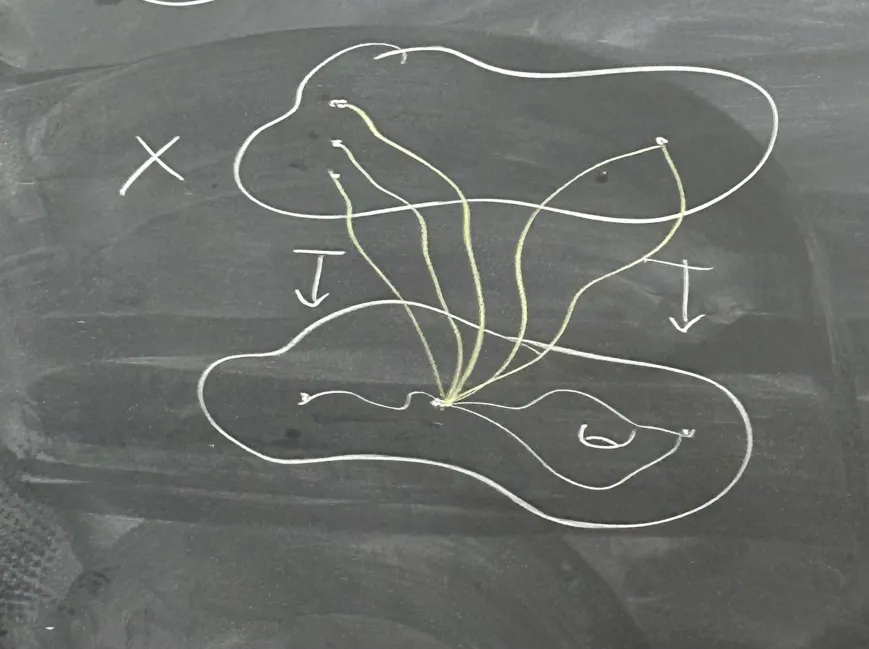
\includegraphics[width=0.35\textwidth]{Figures/homotopy_fiber.png}\]
\end{remark}

\begin{theorem}
    If $X$ and $Y$ are ``nice" (ex. connected CW complexes), $f: X \to Y$ is a map, $\operatorname{hofib}_f(y) \simeq *$, then $f$ is an equivalence from $X \to Y$.
\end{theorem}

Comma categories is the analog of a ``directed homotopy fiber" for categories.
\begin{definition}
    Let $F: C \to D$ be a functor and $d \in D$, the \textbf{comma category} $d\downarrow F$ has:
    \begin{itemize}
        \item Objects: Maps $\alpha: d \to Fc \in D$.
        \item Morphisms: Triangles of the form
        % https://q.uiver.app/#q=WzAsMyxbMCwxLCJkIl0sWzEsMCwiRmMiXSxbMSwxLCJGYyciXSxbMSwyLCJGZiJdLFswLDEsIlxcYWxwaGEiXSxbMCwyLCJcXGFscGhhJyIsMl1d
\[\begin{tikzcd}
	& Fc \\
	d & {Fc'}
	\arrow["Ff", from=1-2, to=2-2]
	\arrow["\alpha", from=2-1, to=1-2]
	\arrow["{\alpha'}"', from=2-1, to=2-2]
\end{tikzcd}\]
    \end{itemize}
    We also define $F \downarrow d$ dually (ie. the arrows go the other way).
\end{definition}

\begin{definition}
    Let $M$ is a monoid acting on a set $X$, the \textbf{translation category} $M \int X$:
    \begin{itemize}
        \item Objects are $X$.
        \item $\operatorname{Hom}(x, y) = \{m \in M: m \cdot x = y\}$.
    \end{itemize}
\end{definition}

\begin{example}
\begin{itemize}
    \item Let $F$ be the identity functor on $D$, then $d \downarrow F$ is the slice category of $D$ on $d$, and $F \downarrow d$ is the co-slice category of $D$ on $d$.
    \item Let $M$ and $N$ be monoids, viewed as a category with 1 element. If $\iota: M \hookrightarrow N$ is an inclusion of commutative monoids, then $\iota \downarrow *$ is the translation category $M \int N$.
\end{itemize}
\end{example}

Now we see why comma categories should be the analog of homotopy fibers.
\begin{theorem}[Quillen's Theorem A]
    If $F: C \to D$ is a functor such that $F \downarrow d$ is contractible for all $d$, then $BF: BC \to BD$ is an equivalence.
\end{theorem}

\begin{remark}
    This theorem need not require $d \downarrow F$ to be contractible, we only needed to check one direction.
\end{remark}

\begin{corollary}
    Consider the inclusion of a commutative monoid $M$ into its group completion $M^{gp}$, this induces an equivalence $BM \simeq BM^{gp}$ (where we view a commutative monoid as a category with one object).
\end{corollary}

\begin{proof}
    Consider the inclusion of a commutative monoid $M$ into its group completion $M^{gp}$, then the comma category $i \downarrow *$ is the translation category $M \int M^{gp}$.\\

    We can check that this category is filtered and hence contractible. Thus, Quillen's Theorem $A$ implies the inclusion map $M \to M^{gp}$ induces an equivalence $BM \simeq BM^{gp}$. Let us check this is filtered. Indeed, for condition (1): for $[m_1] - [n_1], [m_2] - [n_2] \in M^{gp}$, we can add $[n_1] + [m_2]$ and $[n_2] + [m_1]$ to the first and second term respectively to get:
    % https://q.uiver.app/#q=WzAsMyxbMCwwLCJbbV8xXSAtIFtuXzFdIl0sWzAsMiwiW21fMl0gLSBbbl8yXSJdLFsxLDEsIlttXzFdICsgW21fMl0iXSxbMCwyLCIrKFtuXzFdICsgW21fMl0pIiwxXSxbMSwyLCIrKFtuXzJdICsgW21fMV0pIiwxXV0=
\[\begin{tikzcd}
	{[m_1] - [n_1]} \\
	& {[m_1] + [m_2]} \\
	{[m_2] - [n_2]}
	\arrow["{+([n_1] + [m_2])}"{description}, from=1-1, to=2-2]
	\arrow["{+([n_2] + [m_1])}"{description}, from=3-1, to=2-2]
\end{tikzcd}\]
    For condition (2), given maps $k, \ell: [m] - [n] \to [m'] \to [n']$ (by $+ [k]$ and $+ [\ell]$). The cancellation property in group completion implies that $[k] \sim [\ell]$ in $M^{gp}$. Thus, there exists $h$ such that $[k] + [h] = [\ell] + [h]$, which concludes the proof.
\end{proof}

\begin{example}
    Let $(\Nbb, +)$ be the natural numbers (including zero) with addition, then $B\Nbb \simeq S^1$.
\end{example}

\begin{question}
    Let $F: C \to D$ be a functor, the composite $d \downarrow F \to C \to  D$ is constant at $d$, thus the induced composition
    \[B(d \downarrow F) \to B(C) \to B(D)\]
    is null-homotopic. This then induces a map $B(d \downarrow F) \to \operatorname{hofib}_{BF}(d)$. Similarly, we have a map $B(F \downarrow d) \to \operatorname{hofib}_{BF}(d)$. Thus, we have natural maps
    % https://q.uiver.app/#q=WzAsMyxbMCwwLCJCKGRcXGRvd25hcnJvdyBGKSJdLFsxLDEsIlxcb3BlcmF0b3JuYW1le2hvZmlifV97QkZ9KGQpIl0sWzIsMCwiQihGIFxcZG93bmFycm93IGQpIl0sWzAsMV0sWzIsMV1d
\[\begin{tikzcd}
	{B(d\downarrow F)} && {B(F \downarrow d)} \\
	& {\operatorname{hofib}_{BF}(d)}
	\arrow[from=1-1, to=2-2]
	\arrow[from=1-3, to=2-2]
\end{tikzcd} \quad (\dagger).\]
When are these equivalences?
\end{question}

\begin{proposition}
    A path $p: y \to y'$ induces an equivalences between $\operatorname{hofib}(y)$ and $\operatorname{hofib}(y')$, given by maps
    \[p_*: \operatorname{hofib}_f(y) \to \operatorname{hofib}_f(y') \text{ and } p^*: \operatorname{hofib}_f(y') \to \operatorname{hofib}_f(y). \]
\end{proposition}

Similarly, we have that.
\begin{proposition}
    A map $f: d \to d'$ induces maps
    \[f_*: F\downarrow d \to F \downarrow d' \text{ and } f^*: d'\downarrow F \to d \downarrow F.\]
\end{proposition}

\begin{theorem}[Quillen's Theorem B]
    If the maps $f_*$ are homotopy equivalences for all $f: d \to d' \in D$, then $(\dagger)$ is a homotopy equivalence. In particular, we have a LES
    \[... \to \pi_{n+1} BD \to \pi_n B(F \downarrow d) \to \pi_n(BC) \to \pi_n(BD) \to ... \]
\end{theorem}

\begin{remark}
    Again, we only checked one direction. If we use $f^*$ instead, we have a LES
        \[... \to \pi_{n+1} BD \to \pi_n B(d \downarrow F) \to \pi_n(BC) \to \pi_n(BD) \to ... \]
\end{remark}

\begin{example}
    Let $i: H \hookrightarrow G$ be an inclusion of groups. In this case, we have that $i \downarrow * \cong H \int G$ is $G/H$. Any $x \in G$ induces an isomorphism $i \downarrow * \to i \downarrow x$, in which case 
    \[\operatorname{hofib}_{Bi} = H \int G \simeq G/H.\]
    Quillen's Theorem B recovers the normal long exact sequence from group (co)homology.
\end{example}

\newpage
\section{Lecture March 20th, 2025 - Yaojie Hu}\label{sec::q_construction}

\textbf{Title:} Q-Construction, Fundamental Theorems, and the K-Theory of Schemes\\

The original paper for this lecture is based on is \cite{quillen_1}. A very helpful treatment of the content is in \cite{Srinivas_1996}.

\subsection{The Q-Construction of Exact Categories}

The Q-construction is a step that takes in an exact category $\Ccal$ and produces a category $Q\Ccal$. It is an important step in giving an alternative (and more general) definition of K-theory for exact categories. An exact category $\Ccal$ intuitively is looking to caputre short exact sequences (SES) of the form $0 \to A \to B \to C \to 0$.

\begin{definition}
An \textbf{exact category} $\Ccal$ is an additive category embedded as a full sub-category of an abelian category $\mathcal{A}$ such that $\Ccal$ is closed under extension, meaning that if $0 \to A \to B \to C \to 0$ is a SES in $\mathcal{A}$, $A, C \in \Ccal$, then $B$ is isomorphic to some object in $\Ccal$. An exact sequence of $\Ccal$ is an exact sequence of $\mathcal{A}$ whose terms are all in $\Ccal$.
\end{definition}

We do not want to consider any functor between exact categories, but rather functors that respect the exactness condition.
\begin{definition}
    A functor $F: \Ccal \to \Dcal$ between exact categories is \textbf{exact} if it is an additive functor that preserves SESs (ie. if $0 \to A \to B \to C \to 0$ is exact in $\Ccal$ then $0 \to F(A) \to F(B) \to F(C) \to 0$ is exact in $\Dcal$). 
\end{definition}

Given an exact category, we can define the $K_0$ group as follows.
\begin{definition}
    The $K_0$ group of an exact category $\Ccal$ is the quotient $F/R$ where $F$ is the free abelian group on $\operatorname{obj}(\Ccal)$ and $R$ is the generated by the relations
    \[[B] - [A] - [C] \text{ for exact sequences } 0 \to A \to B \to C \to 0.\]
\end{definition}

Now we will introduce the Q-construction.
\begin{definition}[Quillen's Q-Construction]
    Let $\Ccal$ be an exact category, we define a category $Q\Ccal$ such that:
    \begin{itemize}
        \item $\operatorname{obj}(Q\Ccal) = \operatorname{obj}(\Ccal)$.
        \item For $X, Y \in \operatorname{obj}(Q\Ccal)$, a morphism $X \to Y$ is an isomorphism class of diagram
        % https://q.uiver.app/#q=WzAsMyxbMCwwLCJYIl0sWzEsMCwiWiJdLFsyLDAsIlkiXSxbMSwwLCJxIiwyLHsic3R5bGUiOnsiaGVhZCI6eyJuYW1lIjoiZXBpIn19fV0sWzEsMiwiaSIsMCx7InN0eWxlIjp7InRhaWwiOnsibmFtZSI6Im1vbm8ifX19XV0=
\[\begin{tikzcd}
	X & Z & Y
	\arrow["q"', two heads, from=1-2, to=1-1]
	\arrow["i", tail, from=1-2, to=1-3]
\end{tikzcd}\]
where $i$ is an \textbf{admissible monomorphism} and $q$ is an \textbf{admissible epimorphism}.
    \end{itemize}
    We will now explain how the morphisms work in detail. A diagram of the form
            % https://q.uiver.app/#q=WzAsMyxbMCwwLCJYIl0sWzEsMCwiWiJdLFsyLDAsIlkiXSxbMSwwLCJxIiwyLHsic3R5bGUiOnsiaGVhZCI6eyJuYW1lIjoiZXBpIn19fV0sWzEsMiwiaSIsMCx7InN0eWxlIjp7InRhaWwiOnsibmFtZSI6Im1vbm8ifX19XV0=
\[\begin{tikzcd}
	X & Z & Y
	\arrow["q"', two heads, from=1-2, to=1-1]
	\arrow["i", tail, from=1-2, to=1-3]
\end{tikzcd} \quad (\dagger)\]
is the data of two exact sequences
\[0 \to Z \xrightarrow{i} Y \to Y' \to 0 \text{ and } 0 \to X' \to Z \xrightarrow{q} X \to 0.\]
In particular, $i$ is a monomorphism and $q$ is an epimorphism in $\Ccal$ (given a monomorphism and epimorphism, we can always recover the two exact sequences above as well). Consider a second diagram of the form 
\[\begin{tikzcd}
	X & Z' & Y
	\arrow["q'"', two heads, from=1-2, to=1-1]
	\arrow["i'", tail, from=1-2, to=1-3]
\end{tikzcd} \quad (\spadesuit).\]
We say $(\dagger)$ and $(\spadesuit)$ are isomorphic if there exists an isomorphism $h: Z \to Z'$ such that the following diagram commutes:
% https://q.uiver.app/#q=WzAsNCxbMSwwLCJaIl0sWzEsMiwiWiciXSxbMCwxLCJYIl0sWzIsMSwiWSJdLFswLDEsImgsIFxcY29uZyJdLFswLDIsInEiLDIseyJzdHlsZSI6eyJoZWFkIjp7Im5hbWUiOiJlcGkifX19XSxbMSwyLCJxJyIsMCx7InN0eWxlIjp7ImhlYWQiOnsibmFtZSI6ImVwaSJ9fX1dLFswLDMsImkiLDAseyJzdHlsZSI6eyJ0YWlsIjp7Im5hbWUiOiJtb25vIn19fV0sWzEsMywiaSciLDJdXQ==
\[\begin{tikzcd}
	& Z \\
	X && Y \\
	& {Z'}
	\arrow["q"', two heads, from=1-2, to=2-1]
	\arrow["i", tail, from=1-2, to=2-3]
	\arrow["{h, \cong}", from=1-2, to=3-2]
	\arrow["{q'}", two heads, from=3-2, to=2-1]
	\arrow["{i'}"', from=3-2, to=2-3]
\end{tikzcd}.\]
The \textbf{identity} morphism of $X \to X$ in $Q\Ccal$ is given by $X \twoheadleftarrow_{id_X} X \rightarrowtail_{id_X} X$. Given two morphisms $X \twoheadleftarrow Z \rightarrowtail Y$ and $Y \twoheadleftarrow V \rightarrowtail T$, we define a \textbf{composition}:
\[\begin{tikzcd}
	X & W & T
	\arrow["f"', two heads, from=1-2, to=1-1]
	\arrow["g", tail, from=1-2, to=1-3]
\end{tikzcd}\]
by considering the following:
% https://q.uiver.app/#q=WzAsNixbMCwwLCJYIl0sWzEsMSwiWSJdLFsyLDIsIlQiXSxbMCwxLCJaIl0sWzEsMiwiViJdLFswLDIsIlcgXFxjb2xvbmVxcSBaIFxcdGltZXNfWSBWIl0sWzMsMCwicSIsMCx7InN0eWxlIjp7ImhlYWQiOnsibmFtZSI6ImVwaSJ9fX1dLFszLDEsImkiLDAseyJzdHlsZSI6eyJ0YWlsIjp7Im5hbWUiOiJtb25vIn19fV0sWzQsMSwicSciLDIseyJzdHlsZSI6eyJoZWFkIjp7Im5hbWUiOiJlcGkifX19XSxbNCwyLCJpJyIsMix7InN0eWxlIjp7InRhaWwiOnsibmFtZSI6Im1vbm8ifX19XSxbNSwzLCJmJyJdLFs1LDQsImcnIiwyXV0=
\[\begin{tikzcd}
	X \\
	Z & Y \\
	{W \coloneqq Z \times_Y V} & V & T
	\arrow["q", two heads, from=2-1, to=1-1]
	\arrow["i", tail, from=2-1, to=2-2]
	\arrow["{f'}", from=3-1, to=2-1]
	\arrow["{g'}"', from=3-1, to=3-2]
	\arrow["{q'}"', two heads, from=3-2, to=2-2]
	\arrow["{i'}"', tail, from=3-2, to=3-3]
\end{tikzcd}\]
Here $(W, f', g')$ is constructed from the pull-back and we specify
\[f \coloneqq q \circ f' \text{ and } g = i' \circ g'.\]
\ul{One can check that composition respects isomorphism classes and identity and is associative}. Thus, $Q\Ccal$ is a valid category.
\end{definition}

From the construction above, one can immediately see that.
\begin{proposition}
    Let $\Ccal$ be a small exact category, then $Q\Ccal$ is a small category.
\end{proposition}

Before we move on to defining the higher K-theories, let us first establish some terminologies and tools in the Q-construction.
\begin{definition}
    Let $i: M \rightarrowtail N$ be a monomorphism in $\Ccal$, we define an associated morphism $i_!: M \to N$ in $Q\Ccal$ of the form:
    \[\begin{tikzcd}
	M & M & N
	\arrow["id_{M}"', two heads, from=1-2, to=1-1]
	\arrow["i", tail, from=1-2, to=1-3]
\end{tikzcd}.\]
    Let $q: M \twoheadrightarrow N$ be an epimorphism in $\Ccal$, we define an associated morphism $q^!: N \to M$ in $Q\Ccal$ of the form
        \[\begin{tikzcd}
	N & M & M
	\arrow["q"', two heads, from=1-2, to=1-1]
	\arrow["id_{M}", tail, from=1-2, to=1-3]
\end{tikzcd}.\]
\end{definition}

\begin{proposition}
    Let $f: M \to N$ be a morphism in $Q\Ccal$, given by
    \[\begin{tikzcd}
	M & M' & N
	\arrow["q"', two heads, from=1-2, to=1-1]
	\arrow["i", tail, from=1-2, to=1-3]
\end{tikzcd}\]
    we can decompose $f = i_! \circ q^!$. Furthermore, if we take the pushout square:
% https://q.uiver.app/#q=WzAsNCxbMCwwLCJNJyJdLFswLDEsIk0iXSxbMSwwLCJOIl0sWzEsMSwiTiciXSxbMCwxLCJxIiwyLHsic3R5bGUiOnsiaGVhZCI6eyJuYW1lIjoiZXBpIn19fV0sWzAsMiwiaSIsMCx7InN0eWxlIjp7InRhaWwiOnsibmFtZSI6Im1vbm8ifX19XSxbMSwzLCJpJyIsMix7InN0eWxlIjp7InRhaWwiOnsibmFtZSI6Im1vbm8ifX19XSxbMiwzLCJxJyIsMCx7InN0eWxlIjp7ImhlYWQiOnsibmFtZSI6ImVwaSJ9fX1dXQ==
\[\begin{tikzcd}
	{M'} & N \\
	M & {N'}
	\arrow["i", tail, from=1-1, to=1-2]
	\arrow["q"', two heads, from=1-1, to=2-1]
	\arrow["{q'}", two heads, from=1-2, to=2-2]
	\arrow["{i'}"', tail, from=2-1, to=2-2]
\end{tikzcd}\quad (\dagger)\]
    We also have that $f = (q')^! \circ i_!'$.
\end{proposition}

\begin{proof}
    To show that $f = i_! \circ q!$, we observe that the composition gives:
    % https://q.uiver.app/#q=WzAsNixbMCwxLCJNIl0sWzEsMSwiTSJdLFswLDAsIk4iXSxbMSwyLCJNIl0sWzIsMiwiTiJdLFswLDIsIk0gXFx0aW1lc197TX0gTSJdLFswLDEsImlkX00iLDAseyJzdHlsZSI6eyJ0YWlsIjp7Im5hbWUiOiJtb25vIn19fV0sWzAsMiwicSIsMCx7InN0eWxlIjp7ImhlYWQiOnsibmFtZSI6ImVwaSJ9fX1dLFszLDEsImlkX00iLDIseyJzdHlsZSI6eyJoZWFkIjp7Im5hbWUiOiJlcGkifX19XSxbMyw0LCJpIiwwLHsic3R5bGUiOnsidGFpbCI6eyJuYW1lIjoibW9ubyJ9fX1dLFs1LDBdLFs1LDNdXQ==
\[\begin{tikzcd}
	N \\
	M & M \\
	{M \times_{M} M} & M & N
	\arrow["q", two heads, from=2-1, to=1-1]
	\arrow["{id_M}", tail, from=2-1, to=2-2]
	\arrow[from=3-1, to=2-1]
	\arrow[from=3-1, to=3-2]
	\arrow["{id_M}"', two heads, from=3-2, to=2-2]
	\arrow["i", tail, from=3-2, to=3-3]
\end{tikzcd}\]
In this case we see that the pullback $M \times_M M \cong M$ and the two maps going out of the pullback are identity maps. Thus, the composition equals to $f$.\\

Now to show that $(q')^! \circ (i')_! = f$, we see that the composition gives the diagram:
% https://q.uiver.app/#q=WzAsNixbMCwxLCJNIl0sWzEsMSwiTiciXSxbMCwwLCJNIl0sWzEsMiwiTiJdLFsyLDIsIk4iXSxbMCwyLCJNIFxcdGltZXNfe04nfSBOIl0sWzAsMSwiaSciLDAseyJzdHlsZSI6eyJ0YWlsIjp7Im5hbWUiOiJtb25vIn19fV0sWzMsMSwicSciLDIseyJzdHlsZSI6eyJoZWFkIjp7Im5hbWUiOiJlcGkifX19XSxbMyw0LCJpZF9OIiwwLHsic3R5bGUiOnsidGFpbCI6eyJuYW1lIjoibW9ubyJ9fX1dLFs1LDBdLFs1LDNdLFswLDIsImlkX00iLDAseyJzdHlsZSI6eyJoZWFkIjp7Im5hbWUiOiJlcGkifX19XV0=
\[\begin{tikzcd}
	M \\
	M & {N'} \\
	{M \times_{N'} N} & N & N
	\arrow["{id_M}", two heads, from=2-1, to=1-1]
	\arrow["{i'}", tail, from=2-1, to=2-2]
	\arrow[from=3-1, to=2-1]
	\arrow[from=3-1, to=3-2]
	\arrow["{q'}"', two heads, from=3-2, to=2-2]
	\arrow["{id_N}", tail, from=3-2, to=3-3]
\end{tikzcd}\]
We note that the square in $(\dagger)$ is \textbf{bi-Cartesian}, ie. it is both a pushout and pullback diagram. Thus, we can replace the diagram above as:
% https://q.uiver.app/#q=WzAsNixbMCwxLCJNIl0sWzEsMSwiTiciXSxbMCwwLCJNIl0sWzEsMiwiTiJdLFsyLDIsIk4iXSxbMCwyLCJNJyJdLFswLDEsImknIiwwLHsic3R5bGUiOnsidGFpbCI6eyJuYW1lIjoibW9ubyJ9fX1dLFszLDEsInEnIiwyLHsic3R5bGUiOnsiaGVhZCI6eyJuYW1lIjoiZXBpIn19fV0sWzMsNCwiaWRfTiIsMCx7InN0eWxlIjp7InRhaWwiOnsibmFtZSI6Im1vbm8ifX19XSxbNSwwLCJxIiwwLHsic3R5bGUiOnsiaGVhZCI6eyJuYW1lIjoiZXBpIn19fV0sWzUsMywiaSIsMix7InN0eWxlIjp7InRhaWwiOnsibmFtZSI6Im1vbm8ifX19XSxbMCwyLCJpZF9NIiwwLHsic3R5bGUiOnsiaGVhZCI6eyJuYW1lIjoiZXBpIn19fV1d
\[\begin{tikzcd}
	M \\
	M & {N'} \\
	{M'} & N & N
	\arrow["{id_M}", two heads, from=2-1, to=1-1]
	\arrow["{i'}", tail, from=2-1, to=2-2]
	\arrow["q", two heads, from=3-1, to=2-1]
	\arrow["i"', tail, from=3-1, to=3-2]
	\arrow["{q'}"', two heads, from=3-2, to=2-2]
	\arrow["{id_N}", tail, from=3-2, to=3-3]
\end{tikzcd}\]
Hence, we have that $(q')^! \circ (i')_! = i_! \circ q^!$, which concludes the proof.
\end{proof}

As a consequence of the proposition, we have the following.
\begin{corollary}
We have the following:
\begin{enumerate}
    \item Let $i: Y \to Z$ and $i': X \to Y$ be admissible monomorphisms in $\Ccal$, then $(i \circ i')_! = i_! \circ (i')_!$.
    \item Let $q: Y \to Z$ and $q': X \to Y$ be admissible epimorphisms in $\Ccal$, then $(q \circ q')^! = (q')^! \circ q^!$.
    \item Suppose we have a \textbf{bi-Cartesian} square of the form:
    % https://q.uiver.app/#q=WzAsNCxbMCwwLCJNJyJdLFsxLDAsIk4iXSxbMCwxLCJNIl0sWzEsMSwiTiciXSxbMCwxLCJpIiwwLHsic3R5bGUiOnsidGFpbCI6eyJuYW1lIjoibW9ubyJ9fX1dLFsyLDMsImknIiwyLHsic3R5bGUiOnsidGFpbCI6eyJuYW1lIjoibW9ubyJ9fX1dLFswLDIsInEiLDIseyJzdHlsZSI6eyJoZWFkIjp7Im5hbWUiOiJlcGkifX19XSxbMSwzLCJxJyIsMCx7InN0eWxlIjp7ImhlYWQiOnsibmFtZSI6ImVwaSJ9fX1dXQ==
\[\begin{tikzcd}
	{M'} & N \\
	M & {N'}
	\arrow["i", tail, from=1-1, to=1-2]
	\arrow["q"', two heads, from=1-1, to=2-1]
	\arrow["{q'}", two heads, from=1-2, to=2-2]
	\arrow["{i'}"', tail, from=2-1, to=2-2]
\end{tikzcd}\]
then we have that $i_! \circ q^! = (q')^! \circ (i')_!$.
\end{enumerate}
\end{corollary}

\begin{proof}
    The last point (3) can be seen directly by applying almost the same proof as the previous proposition. The proofs for (1) and (2) are similar, so we will only show the case for (1). Indeed, we clearly have a composition of the form:
    % https://q.uiver.app/#q=WzAsNixbMCwyLCJYIFxcdGltZXNfWSBZIl0sWzAsMSwiWCJdLFsxLDEsIlkiXSxbMSwyLCJZIl0sWzIsMiwiWiJdLFswLDAsIlgiXSxbMSwyLCJpJyIsMCx7InN0eWxlIjp7InRhaWwiOnsibmFtZSI6Im1vbm8ifX19XSxbMSw1LCJpZF9YIiwwLHsic3R5bGUiOnsiaGVhZCI6eyJuYW1lIjoiZXBpIn19fV0sWzMsNCwiaSIsMCx7InN0eWxlIjp7InRhaWwiOnsibmFtZSI6Im1vbm8ifX19XSxbMywyLCJpZF9ZIiwyLHsic3R5bGUiOnsiaGVhZCI6eyJuYW1lIjoiZXBpIn19fV0sWzAsMV0sWzAsM11d
\[\begin{tikzcd}
	X \\
	X & Y \\
	{X \times_Y Y} & Y & Z
	\arrow["{id_X}", two heads, from=2-1, to=1-1]
	\arrow["{i'}", tail, from=2-1, to=2-2]
	\arrow[from=3-1, to=2-1]
	\arrow[from=3-1, to=3-2]
	\arrow["{id_Y}"', two heads, from=3-2, to=2-2]
	\arrow["i", tail, from=3-2, to=3-3]
\end{tikzcd}\]
By examining the fibered product, we can suitably replace the diagram with:
% https://q.uiver.app/#q=WzAsNixbMCwyLCJYIl0sWzAsMSwiWCJdLFsxLDEsIlkiXSxbMSwyLCJZIl0sWzIsMiwiWiJdLFswLDAsIlgiXSxbMSwyLCJpJyIsMCx7InN0eWxlIjp7InRhaWwiOnsibmFtZSI6Im1vbm8ifX19XSxbMSw1LCJpZF9YIiwwLHsic3R5bGUiOnsiaGVhZCI6eyJuYW1lIjoiZXBpIn19fV0sWzMsNCwiaSIsMCx7InN0eWxlIjp7InRhaWwiOnsibmFtZSI6Im1vbm8ifX19XSxbMywyLCJpZF9ZIiwyLHsic3R5bGUiOnsiaGVhZCI6eyJuYW1lIjoiZXBpIn19fV0sWzAsMSwiaWRfWCIsMCx7InN0eWxlIjp7ImhlYWQiOnsibmFtZSI6ImVwaSJ9fX1dLFswLDMsImknIiwwLHsic3R5bGUiOnsidGFpbCI6eyJuYW1lIjoibW9ubyJ9fX1dXQ==
\[\begin{tikzcd}
	X \\
	X & Y \\
	X & Y & Z
	\arrow["{id_X}", two heads, from=2-1, to=1-1]
	\arrow["{i'}", tail, from=2-1, to=2-2]
	\arrow["{id_X}", two heads, from=3-1, to=2-1]
	\arrow["{i'}", tail, from=3-1, to=3-2]
	\arrow["{id_Y}"', two heads, from=3-2, to=2-2]
	\arrow["i", tail, from=3-2, to=3-3]
\end{tikzcd}\]
which shows the equality $(i \circ i')_! = i_! \circ (i')_!$.
\end{proof}

This corollary actually characterizes $Q\Ccal$ in the following sense.
\begin{lemma}[Characterization of $Q\Ccal$]\label{lem::characterization_QC}
    Let $\Ccal$ be an exact category and $\Dcal$ a category. Suppose we have:
    \begin{itemize}
        \item (i) For each $M \in \Ccal$, we assign an object $F(M) \in \Dcal$.
        \item (ii) For each admissible monomorphism $i: M' \rightarrowtail M$, we can assign a morphism
        \[F_1(i): F(M') \to F(M) \text{ such that } F_1(i \circ i') = F_1(i) \circ F_1(i')\]
        for composable admissible monomorphisms $i$ and $i'$. For each admissible epimorphism $q: M \twoheadrightarrow N$, we can assign a morphism
        \[F_2(q): F(N) \to F(M) \text{ such that } F_q(q \circ q') = F_2(q') \circ F_2(q)\]
        for composable admissible epimorphisms $q$ and $q'$.
        \item For any bi-Cartesian square of the form
        \[\begin{tikzcd}
	{M'} & N \\
	M & {N'}
	\arrow["i", tail, from=1-1, to=1-2]
	\arrow["q"', two heads, from=1-1, to=2-1]
	\arrow["{q'}", two heads, from=1-2, to=2-2]
	\arrow["{i'}"', tail, from=2-1, to=2-2]
\end{tikzcd}\]
we have that $F_1(i) \circ F_2(q) = F_2(q') \circ F_1(i')$.
    \end{itemize}
Then there exists a well-defined functor $F: Q\Ccal \to \Dcal$ such that
\[M \mapsto F(M) \text{ and } M \twoheadleftarrow_{q} M' \rightarrowtail_{i} N \mapsto F_1(i) \circ F_2(q).\]
\end{lemma}

\begin{corollary}
    Let $\Ccal$ be an exact category, then $Q\Ccal$ is isomorphic to $Q(\Ccal^{op})$.
\end{corollary}

\begin{proof}
    Although this was marked as a corollary in the textbook (Srinivas), the proof really does not use the previous lemma. Instead, we define an explicit functor
    \[F: Q\Ccal \to Q(\Ccal^{op})\]
    that is identity on objects and for a morphism $f: M \to N$, we decompose $f = i_! \circ q^!$ and define $F(f) \coloneqq (\overline{q'})_{!} \circ (\overline{i'})^{!}$. Here $q', i'$ are constructed from the bi-Cartesian square in the proposition prior and $\overline{\bullet}$ denotes we are looking at the corresponding map in the opposite category. One can check $F$ gives an isomorphism of categories.
    % Let $\Dcal = \Ccal^{op}$ in this case. For each object $M \in \Ccal$, we assign $F(M) = M$. For an admissible momonomorphism $i: M \to N$, we assign $F_1(i): N \to M$ to be the correspondent map in the opposite category, and similarly to $F_2$
\end{proof}

\begin{proposition}
    Isomorphisms in $Q\Ccal$ are in one-to-one correspondence with isomorphisms in $\Ccal$.
\end{proposition}

\begin{proof}
    Let $f: A \to B$ be an isomorphism in $\Ccal$ and write $f^{-1}: B \to A$. We can construct an isomorphism and its inverse as 
    \[B \twoheadleftarrow_{f} A \rightarrowtail_{id_{A}} A \text{ and } A \twoheadleftarrow_{f^{-1}} B \rightarrowtail_{id_{B}} B.\]
    Conversely, suppose $f: A \to B$ is an isomorphism in $Q\Ccal$, then we can write $f$ and $f^{-1}$ as respective diagrams:
    \[A \twoheadleftarrow_{j} C \rightarrowtail_{i} B \text{ and } B \twoheadleftarrow_{j'} C' \rightarrowtail_{i'} A.\]
    Now consider a diagram of the form:
    % https://q.uiver.app/#q=WzAsOSxbMSwxLCJDIl0sWzIsMSwiQyciXSxbMywxLCJDIl0sWzEsMCwiQiJdLFszLDAsIkEiXSxbMCwzLCJCIl0sWzEsMywiQSJdLFszLDMsIkIiXSxbNCwzLCJBIl0sWzAsNSwiaSIsMl0sWzAsNiwiaiJdLFsxLDYsImknIiwyXSxbMSw3LCJqJyJdLFsyLDcsImkiXSxbMiw4LCJqIl0sWzMsMCwiYiIsMl0sWzMsMSwiYiciXSxbNCwxLCJhJyIsMl0sWzQsMiwiYSJdXQ==
\[\begin{tikzcd}
	& B && A \\
	& C & {C'} & C \\
	\\
	B & A && B & A
	\arrow["b"', from=1-2, to=2-2]
	\arrow["{b'}", from=1-2, to=2-3]
	\arrow["{a'}"', from=1-4, to=2-3]
	\arrow["a", from=1-4, to=2-4]
	\arrow["i"', from=2-2, to=4-1]
	\arrow["j", from=2-2, to=4-2]
	\arrow["{i'}"', from=2-3, to=4-2]
	\arrow["{j'}", from=2-3, to=4-4]
	\arrow["i", from=2-4, to=4-4]
	\arrow["j", from=2-4, to=4-5]
\end{tikzcd}\]
Here the maps $b: B \to C, b': B \to C'$ (resp. $a': A \to C, a: A \to C$) are constructed as follows. We first realize the pullbacks of $j: C \to A$ and $i': C' \to A$ (resp. $j': C' \to B$ and $i: C \to B$) in the definition of composition. On the other hand, since the composition is the identity (this is an isomorphism), we can without loss replace the pullback diagrams with the maps presented here such that $i$ and $b$ are inverses, and $b'$ and $j'$ are inverses. (resp. $i', a'$ are inverses and $j,a$ are inverses).\\

From here we construct a pair of maps
\[i \circ a: A \to B \text{ and } j \circ b: B \to A\]
which we can check are inverses. Indeed,
\begin{align*}
    (i \circ a) \circ (j \circ b) &= i \circ (a \circ j) \circ b\\
    &= i \circ id_{A} \circ b\\
    &= id_{B}.
\end{align*}
Conversely,
\begin{align*}
    (j \circ b) \circ (i \circ a) &= j \circ (b \circ i) \circ a\\
    &= j \circ id_{B} \circ a\\
    &= id_{A}.
\end{align*}
One can check that these two assignments are inverses of each other.
\end{proof}

\begin{theorem}\label{Q_construction_pi1}
Let $\Ccal$ be an exact category, $0 \in \Ccal$ be the zero object and $\{0\}$ be the correspondent object of $Q\Ccal$. There exists a natural isomorphism of $\pi_1(BQ\Ccal, \{0\}) \cong K_0(\Ccal)$.
\end{theorem}

\begin{remark}
Explicitly, the map is described as follows. Let $M \in \Ccal$, then there are two canonical maps $0 \to M$ in $Q\Ccal$ of the form
\[0 \twoheadleftarrow 0 \rightarrowtail M \text{ and } 0 \twoheadleftarrow M \rightarrowtail_{id_M} M\]
These two maps defines a loop $\gamma_M$ based at $\{0\}$ in $BQ\Ccal$. We can define the isomorphism
\[K_0(\Ccal) \to \pi_1(BQ\Ccal, \{0\}), [M] \mapsto [\gamma_{M}].\]
\end{remark}

\begin{proof}[Proof Sketch]
    To prove the theorem, we first assert the following two lemma.
    \begin{lemma}
        Let $X$ be a connected and locally simply-connected space and $x \in X$. There is an equivalence of category between covering spaces over $X$ and $\pi_1(X, x)$-sets.
    \end{lemma}
    
    \begin{lemma}
        Let $\Ccal$ be a small category. There is an equivalence of category between covering spaces over $B\Ccal$ and the category of functors $F: \Ccal \to \operatorname{Set}$ such that $F(u)$ is a bijection for any morphism $u$ of $\Ccal$.
    \end{lemma}
    Using the first lemma, we see that $\operatorname{Cov}(BQ\Ccal)$ is isomorphic to the category of $\pi_1(BQ\Ccal, \{0\})$-sets. Using the second lemma, $\operatorname{Cov}(BQ\Ccal)$ is equivalent to a category $\mathcal{F}$ of functors $F: \Ccal \to \operatorname{Set}$ satisfying the descriptions above.\\

    Let $\mathcal{F}' \subseteq \mathcal{F}$ be a full subcategory of $\mathcal{F}$ spanned by functors $F': Q\Ccal \to \operatorname{Set}$ such that
    \begin{itemize}
        \item $F'(M) = F'(0)$ and $F'(i_!) = 1_{F(0)}$ for any admissible monomorphisms $i: M' \rightarrowtail M$ in $\Ccal$.
    \end{itemize}
    One can show that $\mathcal{F}'$ is equivalent to $\mathcal{F}$ by showing the natural inclusion map $\mathcal{F}' \to \mathcal{F}$ is essentially surjective. Indeed, for any functor $F \in \mathcal{F}$, we can define a functor $F' \in \mathcal{F}'$ such that $F'(M) \coloneqq F(0)$ and for a morphism $u: M \to N$ of the form
    \[\begin{tikzcd}
	M & M' & N
	\arrow["q"', two heads, from=1-2, to=1-1]
	\arrow["i", tail, from=1-2, to=1-3]
\end{tikzcd}\]
we define
\[F'(u) \coloneqq F((i_{M'})_!)^{-1} \circ F(q^!) \circ F((i_{M})_!)\]
Here $i_M$ is the unique map $0 \to M$. The map $M \mapsto F((i_{M})_!)$ gives a natural isomorphism between $F'$ and $F$.\\

One can then show that $\mathcal{F}'$ is equivalent to the category of $K_0(\Ccal)$-sets, which is equivalent to $\operatorname{Cov}(BK_0(\Ccal))$. The chain of equivalences will then imply $\operatorname{Cov}(BQ\Ccal)$ has an initial object (ie. the universal cover) whose automorphism group is $K_0(\Ccal)$. This will then imply the isomorphism between $\pi_1(BQ\Ccal, \{0\})$ and $K_0(\Ccal)$.\\

Now we construct two functors between $K_0(\Ccal)$-sets and $\mathcal{F}'$, which will be an equivalence.\\

Indeed, let $S$ be a $K_0(\Ccal)$-set and $\psi: K_0(\Ccal) \to \operatorname{Aut}(S)$ be the action on $S$. We define an assignment $F_S: Q\Ccal \to \operatorname{Set}$ with
\[F_S(M) = S, (F_S)_1(i_!) = id_S, (F_s)_2(q^!) = \psi([\ker q])\]
(in the sense of Lemma~\ref{lem::characterization_QC}), which then induces the desired functor $F_S: Q\Ccal \to \operatorname{Set}$ as in the lemma.\\
    
Conversely, let $F' \in \mathcal{F}'$. We can create a $K_0(\Ccal)$-set as the pair $(F'(0), \psi_{F'}: K_0(\Ccal) \to \operatorname{Aut}(F(0)))$. Here $\psi_{F'}$ is defined by sending $[M] \mapsto F(q^!_M)$ ($q_M$ is the unique map $M \to 0$).\\

One can check these two maps give the equivalence of categories.
\end{proof}

    % In particular, take $X = BK_0(\Ccal)$, we have that covering spaces of $BK_0(\Ccal)$ are equivalent to the category of $K_0(\Ccal)$-sets. Note that $\Tilde{BK_0(\Ccal)}$ (the universal covering) is an initial object in $\operatorname{Cov}(BK_0(\Ccal))$ with $\operatorname{Aut}(\Tilde{BK_0(\Ccal)}) = K_0(\Ccal)$.\\

    % It suffices for us to show that $\operatorname{Cov}(BQ\Ccal)$ has an initial object with automorphism group $K_0(\Ccal)$.

\subsection{Higher K-theory of Exact Categories, Fundamental Theorems}

Motivated by Theorem~\ref{Q_construction_pi1}, we can now define the higher K-theories as follows.
\begin{definition}
    Let $\Ccal$ be a small exact category, we define
    \[K_i(\Ccal) \coloneqq \pi_{i+1}(BQ\Ccal).\]
    Equivalently we also have that
    \[K_i(\Ccal) \coloneqq \pi_{i}(\Omega BQ\Ccal).\]
    Note that $K_i(\bullet)$ is functorial with respect to exact functors. 
\end{definition}

We are particularly interested in higher K-theory on rings.
\begin{definition}
    Let $R$ be a (not necessarily commutative) ring, $\mathcal{P}(R)$ be the category of finitely generated projective (left) R-modules, $\mathcal{M}(R)$ be the category of finitely generated (left) R-modules.\\

    $\mathcal{P}(R)$ is an exact category without additional assumptions. If $R$ is furthermore Noetherian, then $\mathcal{M}(R)$ is also an exact category. We then define
    \[K_i(R) \coloneqq K_i(\mathcal{P}(R)) \text{ and } G_i(R) = K_i(\mathcal{M}(R)).\]
\end{definition}

\subsubsection{Quotient Category}

Two advantages the Q-construction has over the $+$-construction is that it is functorial and can relate between K-theories of different rings in exact sequences. To discuss this in detail, we need to first introduce the theory of \textbf{quotient categories}.

\begin{definition}[Serre/Thick Subcategory]
    Let $B \subset A$ be an inclusion of an abelian category $B$ as a full additive subcategory of a small abelian category $A$. $B$ is called a \textbf{Serre subcategory} (or a \textbf{thick subcategory}) if for any short exact sequence of the form 
    \[0 \to M \to N \to P \to 0 \text{ in $A$}\]
    $N \in B$ if and only if $M, P \in B$.
\end{definition}

Serre/Thick subcategories are to ideals what abelian categories are to rings.
\begin{definition}[Quotient Category]
Let $B \subset A$ be a Serre sub-category, we can construct a \textbf{quotient category} $A/B$ where:
\begin{itemize}
    \item $\operatorname{obj}(A/B) = \operatorname{obj}(A)$.
    \item Let $M, N$ be objects in $A$, and $M', N'$ be sub-objects of $M$ and $N$ in $B$ (ie. $M' \subset M$ and $N'  \subset N$) with $M/M' \in B$ and $N' \in B$. We have a natural homomorphism
    \[\operatorname{Hom}_A(M, N) \to \operatorname{Hom}_A(M', N/N')\]
    We define
    \[\operatorname{Hom}_{A/B}(M, N) = \operatorname{colim}_{\to (M', N')} \operatorname{Hom}_A(M', N/N')\]
    as $(M', N')$ ranges over all possible pairs of sub-objects satisfying the description above, subject to the ordering $(M', N') \leq (M'', N'')$ if $M'' \subseteq M'$ and $N'' \subseteq N'$.
\end{itemize}
\end{definition}

\begin{example}
    Let $k$ be a field and let $\mathcal{M}(k)$ be the category of all finite dimensional $k$-vector-spaces. This is a thick subcategory of $\operatorname{Mod}(k)$, all $k$-vector spaces.\\

    Consider the quotient $\Ccal = \operatorname{Mod}(k)/\mathcal{M}(k)$, we have that
    \[\operatorname{Hom}_{\Ccal}(X, Y) = \{\text{k-linear maps } X \to Y\}/\{\text{k-linear maps $X \to Y$ with finite dim image}\}\]
\end{example}

\subsubsection{Fundamental Theorems}

In this section we introduce a few tools of computation with the Q-construction definition of higher K-theory. Our emphasis will be on applications of these theorems as opposed to their proofs.

\begin{theorem}[The Resolution Theorem]
    Let $\mathcal{M}$ be an exact category and $\mathcal{P} \subset \mathcal{M}$ a full additive subcategory, closed under extensions in $M$. Note that $\mathcal{P}$ in this case is also exact such that the natural inclusion $i: \mathcal{P} \to \mathcal{M}$ is an exact functor. Suppose that:
    \begin{itemize}
        \item (a) If $0 \to M' \to M \to M'' \to 0$ is exact, $M, M'' \in \mathcal{P}$, then $M' \in \mathcal{P}$.
        \item (b) For any object $M \in \mathcal{M}$, there is a finite resolution of the form
        \[0 \to P_n \to P_{n-1} \to ... \to P_0 \to M \to 0\]
        with $P_i \in \mathcal{P}$.
    \end{itemize}
    Then the induced map $BQ \mathcal{P} \to BQ \mathcal{M}$ by inclusion is a homotopy equivalence. In particular, this implies that $K_i(\mathcal{P}) \cong K_i(\mathcal{M})$.
\end{theorem}

From now on we assume rings are commutative unless stated otherwise.
\begin{corollary}
    Let $R$ be a regular Noetherian ring, then the inclusion map $i: \mathcal{P}(R) \to \mathcal{M}(R)$ induces an isomorphism $K_i(R) \cong G_i(R)$.
\end{corollary}

\begin{proof}
    It is a general commutative algebra fact that projective $R$-modules over regular Noetherian ring $R$ satisfies both $(a)$ and $(b)$ in the Resolution theorem with respect to finitely generated $R$-modules. The corollary then follows.
\end{proof}

\begin{theorem}[Devissage]
    Let $A$ be an Abelian category and $B \subset A$ be a full Abelian subcategory closed under taking sub-objects, quotients, and finite products in $\mathcal{A}$. Suppose for all $M$, there is a finite filtration in $\mathcal{A}$:
    \[0 = M_0 \subset M_1 \subset... \subset M_n = M\]
    with $M_i/M_{i-1} \in B$ for all $i$. It then follows that the natural map $BQ(B) \to BQ(A)$ is a homotopy equivalence, and hence $K_i(B) \cong K_i(A)$.
\end{theorem}

\begin{corollary}
    Let $R$ be a Noetherian ring and $I$ be a nilpotent ideal of $R$, then $G_i(R/I) \cong G_i(R)$.
\end{corollary}

\begin{proof}
   Since $I$ is nilpotent, there exists some $n$ such that $I^n = 0$. Let $M$ be a finitely generated $R$-module, then we have a finite filtration of the form:
   \[0 = I^n M \subset I^{n-1} M \subseteq ... \subseteq IM \subseteq M.\]
   Moreover, we observe that $I^i M/I^{i-1} M$ is still a finitely generated $R/I$-module. Thus, by Devissage theorem, we have that $G_i(R/I) \cong G_i(R)$.
\end{proof}

The following is another corollary of the Devissage theorem. We will not prove the corollary however.
\begin{corollary}\label{cor::split_simple_obj_ki}
    Let $A$ be an abelian category such that every object of $A$ has finite length. Let $\{X_j\ |\ j \in J\}$ be a set of representatives for isomorphism classes of simple objects in $A$, then $K_i(A) \cong \bigoplus_{j \in J} K_i(\operatorname{End}(X_j)^{op})$.
\end{corollary}

\begin{theorem}[The Localization Theorem]
    Let $B$ be a thick full abelian subcategory of $A$ and $C = A/B$ be the associated quotient category. Let $s: B \to A$ and $p: A \to C$ be the natural exact functors, then the induced maps
    \[BQB \xrightarrow{BQ(s)} BQA \xrightarrow{BQ(p)} BQC\]
    is a \textbf{homotopy fibration}. Hence there is an induced long exact sequence og homotopy groups:
    \[... \to K_{i+1}(C) \to K_i(B) \to K_i(A) \to K_i(C) \to ... \to K_0(C) \to 0.\]
\end{theorem}

\begin{corollary}
    Let $R$ be a Dedekind domain and $F = \operatorname{Frac}(R)$ be the field of fraction. Then there is a long exact sequence
    \[... \to K_{i+1}(F) \to \bigoplus_{\pfrak \neq 0 \in \operatorname{Spec}(R)} K_i(R/\pfrak) \to K_i(R) \to K_i(F) \to ...\]
\end{corollary}

\begin{proof}[Proof Sketch]
    To prove the corollary, we first cite the following general fact about quotient categories.
    \begin{lemma}
        Let $R$ be a ring and $S$ a multiplicative subset of $R$. Let $A$ be the category of finitely generated $R$-modules and $B$ be the full subcategory of modules $M$ such that for any $m \in M$, there exists some $s \in S$ such that $s \cdot m = 0$. Then $B$ is a thick subcategory and there is an equivalence of category between $A/B$ and the category of $S^{-1} R$-modules.
    \end{lemma}
    In this case, we choose $S = R - \{0\}$ and see that $A/B$ is equivalent to the category of $F$-vector spaces. Thus, by the localization theorem and resolution theorem (saying there is no difference between $G_i$ and $K_i$ on Noetherian rings), we have an exact sequence: 
    \[... \to K_{i+1}(F) \to K_i(B) \to K_i(R) \to K_i(F) \to ...\]
    The isomorphism between $K_i(B)$ and $\bigoplus_{\pfrak \neq 0 \in \operatorname{Spec}(R)} K_i(R/\pfrak)$ comes from Corollary~\ref{cor::split_simple_obj_ki}.
\end{proof}

Finally, we state the following theorem without proof.
\begin{theorem}[Fundamental Theorem of Rings]
    Let $A$ be a Noetherian ring, then for $i \geq 0$ we have natural isomorphisms of the form:
    \begin{enumerate}
        \item $G_i(A) \cong G_i(A[t])$, induced by change of rings.
        \item $G_i(A[t, t^{-1}]) \cong G_i(A) \oplus G_{i-1}(A)$, where $G_{-1}(A) \coloneqq 0$.
    \end{enumerate}
\end{theorem}

By the resolution theorem, we have that:
\begin{corollary}
    Let $A$ be a Noetherian regular ring, then for $i \geq 0$ we have natural isomorphisms of the form:
    \begin{enumerate}
        \item $K_i(A) \cong K_i(A[t])$, induced by change of rings.
        \item $K_i(A[t, t^{-1}]) \cong K_i(A) \oplus K_{i-1}(A)$, where $K_{-1}(A) \coloneqq 0$.
    \end{enumerate}
\end{corollary}

\subsection{K-theory of Schemes}

A scheme is to a manifold what a ring is to a Euclidean chart. 

\begin{definition}
    Let $X$ be an arbitrary scheme, we let $\mathcal{P}(X)$ denote the category of locally free sheaves of finite rank on $X$. Note that $\mathcal{P}(X)$ is a full subcategory of the abelian category of quasi-coherent sheaves of $\mathcal{O}_X$-modules over $X$. This realizes $\mathcal{P}(X)$ as an exact category, from which we define
    \[K_i(X) \coloneqq K_i(\mathcal{P}(X)).\]
    Let $\mathcal{M}(X)$ be the category of coherent sheaves over $X$. If $X$ is furthermore Noetherian, then $\mathcal{M}(X)$ is also exact, from which we define
    \[G_i(X) \coloneqq K_i(\mathcal{M}(X)).\]
\end{definition}

\ul{From now on, we assume in this section that a scheme $X$ is always Noetherian and separated unless otherwise stated.} In this case, we can still apply the resolution theorem to obtain an analogous result.

\begin{proposition}
    Suppose $X$ is furthermore regular, then $K_i(X) \cong G_i(X)$ for all $i$.
\end{proposition}

\begin{proof}
    Since $X$ is Noetherian regular, every coherent sheaf is a quotient of a locally free sheaf of finite rank. Thus, we can obtain a finite resolution by locally free sheaf, and the resolution theorem implies $K_i(X) \cong G_i(X)$.
\end{proof}

There are suitable functoriality properties the K-theory of schemes satisfies.
\begin{proposition}
Let $f: X \to Y$ be a morphism between (not necessarily Noetherian) schemes, then $f^*: \mathcal{P}(Y) \to \mathcal{P}(X)$ is exact (by the preimage sheaf) and hence gives a homomorphism $f^*: K_i(Y) \to K_i(X)$. Suppose $f: X \to Y$ is a \textbf{flat morphism} between Noetherian schemes, then $f^*: \mathcal{M}(Y) \to \mathcal{M}(X)$ is exact and hence induces a map $f^*: G_i(Y) \to G_i(X)$.
\end{proposition}

\begin{proof}[Proof Sketch]
A map $f^*: \mathcal{M}(Y) \to \mathcal{M}(X)$ still exists (ie. the pullback of a coherent sheaf is coherent) if $X$ and $Y$ are more generally locally Noetherian. The flatness is needed here to ensure the map is exact. Algebraically, this requirement makes a lot of sense. A flat morphism $g: \operatorname{Spec} R \to \operatorname{Spec} S$ between affine schemes is flat if, by definition, the induced functor sending an $S$-module $M$ to $M \otimes_S R$ (as an $R$-module) is exact.\\

This also gives an explanation (not exactly a proof) as to why the map $f^*: \mathcal{P}(Y) \to \mathcal{P}(X)$ is exact for any morphism $f$. A module over a Noetherian ring is flat if and only if it is locally free, so the tensor product is automatically exact. The non-Noetherian case requires a separate discussion. %https://mathoverflow.net/questions/33522/flatness-and-local-freeness
\end{proof}

This functoriality is also compatible with colimits, that is:
\begin{proposition}
    Let  $i \mapsto X_i$ be a filtered inverse system of (not necessarily Noetherian) schemes where each map $X_i \to X_j$ in the inverse system is affine. Write $X = \lim_{\to} X_i$, then
    \[K_q(X) = \lim_{\to} K_q(X_i).\]
    Similarly, if $X$ and $X_i$ are furthermore Noetherian and the transition maps are flat, then
    \[G_q(X) = \lim_{\to} G_q(X_i).\]
\end{proposition}

We would also expect some results for rings to also hold for schemes. Let $i: Z \to X$ be a closed subscheme and $j: U \to X$ be the open complement. Let $I_Z$ be the sheaf of ideals correspondent to the closed subscheme $Z$ in $X$. We can identifiy $M(Z)$ as a full-subcategory of $M(X)$ as sheaves annilated by $I_Z$.

\begin{proposition}
    If $I_Z$ is nilpotent, then $G_i(Z) \cong G_i(X)$.
\end{proposition}

\begin{proof}
    The proof is similar using the Devissage theorem.
\end{proof}

\begin{proposition}
    We have a long exact sequence of the form
    \[... \to G_{i+1}(U) \to G_i(Z) \xrightarrow{i_*} G_i(X) \xrightarrow{j^*} G_i(U) \to ... \]
\end{proposition}

\begin{proof}
Let $B \subset \mathcal{M}(X)$ be the Serre subcategory being the full subcategory of all sheaves $\mathcal{F}$ such that $\mathcal{F}|_{U} \equiv 0$. By Devissage theorem, $K_i(B) \cong G_i(Z)$. One can show that the quotient category $\mathcal{M}(X)/B$ is equivalent to $\mathcal{M}(U)$. Hence the localization theorem yields the long exact sequence:
    \[... \to G_{i+1}(U) \to G_i(Z) \xrightarrow{i_*} G_i(X) \xrightarrow{j^*} G_i(U) \to ... \]
\end{proof}

\subsection{The Brown-Gersten-Quillen (BGQ) Spectral Sequence}

For convention, we say $K_n(\Ccal) = 0$ if $n < 0$.

\begin{theorem}[The BGQ Spectral Sequence]
    Let $X^p \subset X$ be the set of points of codimension $p$ in $X$. There exists a cohomological spectral sequence:
    \[E_1^{p, q}(X) \coloneqq \bigsqcup_{x \in X^p} K_{-p-q}(\kappa(x)) \implies G_{-p-q}(X),\]
    that is convergent when $X$ has finite Krull dimension. Here, $\kappa(x)$ is the residue field. This spectral sequence is contravariant with respect to flat morphisms.
\end{theorem}

\begin{proof}[Proof Sketch]
    $\mathcal{M}(X)$ admits a filtration by Serre subcategories of the form
    \[\mathcal{M}(X) = \mathcal{M}^0(X) \supset \mathcal{M}^1(X)\ ... \supset \mathcal{M}^p(X),\]
    where $\mathcal{M}^i(X)$ is composed of coherent sheaves whose support is subscheme of codimension $\geq i$ in $X$. For each $i$, we have an equivalence of category
    \[\mathcal{M}^p(X)/\mathcal{M}^{p+1}(X) \simeq \bigsqcup_{x \in X^p} A(\mathcal{O}_{x, X})\]
    where $A(\mathcal{O}_{x, X})$ is the category of $\mathcal{O}_{x, X}$-modules of finite length. By the devissage theorem since $\kappa(x)$ is the residue field of $\mathcal{O}_{x, X}$, there is an isomorphism
    \[K_q(\kappa(x)) \cong G_q(\kappa(x)) \cong K_q(\mathcal{A}(\mathcal{O}_{x, X})).\]
    Applying the localization theorem we get a long exact sequence
    \[... \to K_i(\mathcal{M}^{p+1}(X)) \to K_i(\mathcal{M}^p(X)) \to \bigsqcup_{x \in X^p} K_i(\kappa(x)) \to K_{i-1}(\mathcal{M}^{p+1}(X)) \to ... \]
    The rest of the spectral sequence now follows from a standard exact couple argument, as we had seen last semester. 
\end{proof}

The following are some concrete knowledge about how the spectral sequence works.

\begin{proposition}
    Let $X$ be a regular scheme of finite type over a field $k$, then the image of the differential
    \[d_1: \bigsqcup_{x \in X^{p-1}} K_1(\kappa(x)) \to \bigsqcup_{x \in X^p} K_0(\kappa(x)) \cong \bigsqcup_{x \in X^p} \Zbb\]
    in the BGS spectral sequence is precisely the group of codimension $p$-cycles equivalent to $0$. 
\end{proposition}

\begin{corollary}
    Let $X$ be a regular scheme of finite type over a field $k$, $E^{p, -p}_2 \cong \operatorname{CH}^p(X)$.
\end{corollary}

\begin{corollary}[Bloch's Formula]
    Let $X$ be a regular scheme of finite type over a field $k$, then there are natural isomorphisms $H^p(X, \mathcal{K}_{p, X}) \cong \operatorname{CH}^p(X)$. Here, $\mathcal{K}_{p, X}$ is the Zariski sheafification of the presheaf $U \mapsto K_p(U)$. 
\end{corollary}

\newpage
\section{Lecture March 25th, 2025 - Albert Jinghui Yang}

\ul{Title: Plus-construction = Q-construction}
\subsection{Plus-Construction = Q-construction}

Today we will show that Quillen's $+$-construction agrees with Quillen's Q-construction for rings $R$. This is the core of Quillen II (which is atually by Grayson) \cite{quillen_2}. For simplicity, we will assume that $R$ is a \textbf{commutative} ring with identity, but note that the agreement also holds for non-commutative rings.\\

Recall that the plus construction defined
\[K_i(R) \coloneqq \pi_i(\operatorname{BGL}(R)^+) \text{ for } i \geq 1\]
and $K_0(R)$ is defined separately.\\

On the other hand, the Q-construction defines $K_i(R)$ by considering the exact category $\mathcal{C} = \mathcal{P}(R)$ (the category of finitely generated projective $R$-modules). From here, we create another category $Q\mathcal{C}$ and define
\[K_i(R) \coloneqq \pi_i(\Omega B\mathcal{Q}C). \]

Before we prove the theorem, we first introduce some notations.
\begin{definition}
Let $\Ccal$ be a \textbf{split exact category}.
\begin{enumerate}
    \item We let $S = \operatorname{iso} \Ccal$ as the subcategory $\Ccal$ whose objects are the same as $\Ccal$ and morphisms between two objects are the subset composing of isomorphisms. \ul{We also assume} there is a \textbf{symmetric monoidal structure} $\oplus$ on $S$.
    
    \item Let $X$ be a split exact category and $S = \operatorname{iso} X$. We define $S^{-1} X$ as the category whose objects are the pair $(s, x)$ for $s \in S$ and $x \in X$, and a morphism between $(s, x) \to (t, y)$ is a pair of equivalence class of maps
    \[u \oplus s \to t \text{ and } u \oplus x \to y\]
    for some $u \in \operatorname{Obj}(S)$. \ul{In particular, let $X = S$, note that clearly $\operatorname{iso} S = S$, so we can define a category $S^{-1} S$}.

    \item More generally, $S^{-1} X$ can be defined for a symmetric monoidal category $S$ acting on $X$.
\end{enumerate}    
\end{definition}

\begin{remark}
    There is an action of $S$ on $S^{-1} X$ by
    \[s \bullet (t, x) = (t, s \oplus x)\]
    which is invertible.
\end{remark}

Let $\Ccal = \mathcal{P}(R)$ for now, we care about $S^{-1} S$ because its classfying space obtains the K-theory space in the plus construction.
\begin{theorem}
    $B(S^{-1} S)$ is equivalent to $K_0 R \times \operatorname{BGL}(R)^+$.
\end{theorem}

Before we prove the theorem, we introduce a definition.
\begin{definition}
    Let $\Ccal, \Dcal$ be symmetric monoidal categories. A functor $F: \Ccal \to \Dcal$ is \textbf{cofinal} if:
    \begin{enumerate}
        \item $F$ is monoidal.
        \item For all $d \in \Dcal$, there exists $d' \in \mathcal{D}, c \in \Ccal$ such that
        \[d \otimes_{\Dcal} d' \cong F(c).\]
    \end{enumerate}
\end{definition}

\begin{proof}
    The proof of this theorem follows from the following two lemma.
    \begin{lemma}
        Let $\mathcal{F}(R)$ be the category of finitely generated free $R$-modules and $S = \operatorname{iso} \mathcal{F}(R)$, then
        \[B(S^{-1} S) \simeq \Zbb \times \operatorname{BGL}(R)^+.\]
    \end{lemma}

    \begin{proof}[Proof Sketch]
      \textbf{Step 1:} We construct a map $\phi: \operatorname{BGL}(R) \to B(S^{-1} S)_0$, where $B(S^{-1} S)_0$ is the base-component containing $\{0\}$. To define this map, we define maps $\phi_n: \operatorname{BGL}_n(R) \to \operatorname{B} \operatorname{Aut}(R^n) \hookrightarrow B(S^{-1} S)_0$. Then we can show that the following diagram is homotopy-commutative:
      % https://q.uiver.app/#q=WzAsMyxbMCwwLCJcXG9wZXJhdG9ybmFtZXtCR0x9X24oUikiXSxbMCwxLCJcXG9wZXJhdG9ybmFtZXtCR0x9X3tuKzF9KFIpIl0sWzEsMCwiQihTXnstMX0gUylfMCJdLFswLDEsIlxccGhpX24iLDJdLFswLDJdLFsxLDJdXQ==
\[\begin{tikzcd}
	{\operatorname{BGL}_n(R)} & {B(S^{-1} S)_0} \\
	{\operatorname{BGL}_{n+1}(R)}
	\arrow[from=1-1, to=1-2]
	\arrow["{\phi_n}"', from=1-1, to=2-1]
	\arrow[from=2-1, to=1-2]
\end{tikzcd}\]
for all $n$. The universal property then yields a map $\phi: \operatorname{BGL}(R) \to B(S^{-1} S)_0$.\\

\textbf{Step 2:} Show that $\phi$ is acyclic. The upshot here is that $B(S^{-1} S)$ is that
\[H_*(B(S^{-1} S)) = H_*(BS[\frac{1}{e}])\]
for $e = [R] \in \pi_0(S)$ (the homotopy class given by $R$ in $\pi_0(S)$). From here, one can show that
\[H_*(BS[\frac{1}{e}]) = \operatorname{colim} (H_* BS \xrightarrow{\oplus e} H_* BS  \xrightarrow{\oplus e} ... )\]
\[\cong H_* (\operatorname{colim}(BS \xrightarrow{\oplus R} BS \xrightarrow{\oplus R} ...)\]
\[\cong H_* \operatorname{BGL}(R).\]
Details of this can be found in Weibel IV.\\

\textbf{Step 3:} From the previous computation and Whitehead's theorem to show that
\[B(S^{-1} S)_0 \cong \operatorname{BGL}(R)^+.\]
One can show that there is exactly an $\Zbb$ amount of connected components of the form $B(S^{-1} S)_n$ for $n \in \Zbb$ (this has something to do with the fact that the group completion of $\Nbb$ is $\Zbb$). Furthermore, each $B(S^{-1} S)_n$ is equivalent to $B(S^{-1} S)_0$. Hence, we have that
\[B(S^{-1} S) \simeq \Zbb \times \operatorname{BGL}(R)^+.\]

    \end{proof}
Here is the second lemma. The proof of the second lemma is more complicated and will be omitted.
\begin{lemma}[Cofinal Functor Theorem, (Weibel Theorem 4,8, IV)]
    Let $F: \Ccal \to \Dcal$ be a co-final functor. Suppose $\Dcal$ acts on a category $X$, then $\Ccal$ also admits an action on $X$ via $F$. Furthermore, $\Ccal^{-1} X \simeq \Dcal^{-1} X$.
\end{lemma}

Let us see how the theorem follows from the two lemma. Indeed, let $F: \mathcal{F}(R) \to \mathcal{P}(R)$ be the natural inclusion functor. One can show that $F$ is a cofinal functor and hence we have that ...
\end{proof}

Let us proceed in the next step of the proof.
\begin{definition}
Let $\Ccal$ be an exact category. We define $\mathcal{E} \Ccal$ as a category as follows:
\begin{itemize}
    \item Objects: Admissible exact sequence of $\Ccal$ of the form:
    \[A \to B \to C\]
    (Here admissibe exact sequence is just an exact sequence, the adjective is added for extra emphasis).
    
    \item Morphism: Let $E, E'$ be two admissble exact sequence. A morphism $E \to E'$ is the data of % % https://q.uiver.app/#q=WzAsMTEsWzEsMCwiQSJdLFsyLDAsIkIiXSxbMywwLCJDIl0sWzEsMSwiQSciXSxbMSwyLCJBJyJdLFsyLDIsIkInIl0sWzMsMiwiQyciXSxbMiwxLCJCIl0sWzMsMSwiQycnIl0sWzAsMCwiRToiXSxbMCwyLCJFJzoiXSxbMywwLCJcXHRleHR7bW9ub30iLDAseyJzdHlsZSI6eyJ0YWlsIjp7Im5hbWUiOiJob29rIiwic2lkZSI6InRvcCJ9fX1dLFszLDQsIj0iLDJdLFs3LDEsIj0iXSxbNyw1LCJcXHRleHR7ZXBpfSIsMix7InN0eWxlIjp7ImhlYWQiOnsibmFtZSI6ImVwaSJ9fX1dLFs4LDIsIlxcdGV4dHtlcGl9IiwyLHsic3R5bGUiOnsiaGVhZCI6eyJuYW1lIjoiZXBpIn19fV0sWzgsNiwiXFx0ZXh0e21vbm99IiwwLHsic3R5bGUiOnsidGFpbCI6eyJuYW1lIjoiaG9vayIsInNpZGUiOiJ0b3AifX19XSxbMyw3XSxbNyw4XSxbMCwxXSxbMSwyXSxbNCw1XSxbNSw2XV0=
\[\begin{tikzcd}
	{E:} & A & B & C \\
	& {A'} & B & {C''} \\
	{E':} & {A'} & {B'} & {C'}
	\arrow[from=1-2, to=1-3]
	\arrow[from=1-3, to=1-4]
	\arrow["{\text{mono}}", hook, from=2-2, to=1-2]
	\arrow[from=2-2, to=2-3]
	\arrow["{=}"', from=2-2, to=3-2]
	\arrow["{=}", from=2-3, to=1-3]
	\arrow[from=2-3, to=2-4]
	\arrow["{\text{epi}}"', two heads, from=2-3, to=3-3]
	\arrow["{\text{epi}}"', two heads, from=2-4, to=1-4]
	\arrow["{\text{mono}}", hook, from=2-4, to=3-4]
	\arrow[from=3-2, to=3-3]
	\arrow[from=3-3, to=3-4]
\end{tikzcd}\]
such that $A' \to B \to C''$ is an admissble exact sequence.
\end{itemize}
Note that there is an isomorphisn in 
\end{definition}

\begin{definition}
    There is a target functor
    \[t: \mathcal{E} \Ccal \to Q\Ccal, (A \to B \to C) \mapsto C\]
    We also define $\mathcal{E}_c \coloneqq t^{-1}(c)$ for $c \in Q\Ccal$.
\end{definition}

Recall Quillen's Theorem B tells us the following.
\begin{theorem}[Quillen's Theorem B]
    Let $F: \Ccal \to \Dcal$ be a map such that every morphism $f: d \mapsto d'$ induces a homotopy equivalence in the associated base change functor:
    \[f^*: F^{-1}(d') \to d' \downarrow F \to d \downarrow F \to F^{-1} d\]
    then we have a homotopy fibration:
    \[B(d \downarrow F) \to B\Ccal \to B\Dcal\]
\end{theorem}


\begin{theorem}
    There is a fibration of the form
    \[S^{-1} S \to S^{-1} \mathcal{E} \Ccal \to Q \Ccal\]
\end{theorem}

\begin{proof}
    The proof follows from the following lemmas.
    \begin{lemma}
        For all $c \in \Ccal$, $\mathcal{E}_c$ is a symmetric monoidal category, and there is a faithful and monoidal functor
        \[\eta_c: S \coloneqq \operatorname{iso} \Ccal \to \mathcal{E}_c, A \mapsto (A \to A \oplus c \to c).\]
    \end{lemma}

    \begin{lemma}
        If $\Ccal$ is split exact category, then $S^{-1} S \simeq S^{-1} \mathcal{E}_c$ for all $c \in \Ccal$.
    \end{lemma}

    To prove the second lemma, we remark we need the fact that a connected $H$-space is grouplike (ie. its $\pi_0$ is a group). We also need to consider the cofibration
    \[S^{-1} S \to S^{-1} \mathcal{E}_c \to \operatorname{cofib}.\]
    One can show that the cofiber $\operatorname{cofib} = \langle S, \mathcal{E}_c \rangle$ is the category whose objects are the same as $\mathcal{E}_c$ and morphisms are the equivalent classes of pairs
    \[(s, s \otimes E_1 \xrightarrow{\phi} E_2), s \in S, \phi \in \operatorname{Mor}(\mathcal{E}_c)\]
    where $(s_1, \phi_1) \sim (s_2, \phi_2)$ if there is an isomorphism $s_1 \cong s_2$ such that the following diagram commutes:
    % https://q.uiver.app/#q=WzAsMyxbMCwwLCJzXzEgXFxvdGltZXMgRV8xIl0sWzAsMSwic18yIFxcb3RpbWVzIEVfMiJdLFsxLDAsIkVfMiJdLFswLDEsIlxcY29uZyIsMl0sWzEsMiwiXFxwaGlfMiIsMl0sWzAsMiwiXFxwaGlfMSJdXQ==
\[\begin{tikzcd}
	{s_1 \otimes E_1} & {E_2} \\
	{s_2 \otimes E_2}
	\arrow["{\phi_1}", from=1-1, to=1-2]
	\arrow["\cong"', from=1-1, to=2-1]
	\arrow["{\phi_2}"', from=2-1, to=1-2]
\end{tikzcd}\]
    From here one can show that:
    \begin{enumerate}
        \item $\operatorname{cofib}$ is connected. The idea is that for any $E_1, E_2$ we can construct a diagram of the following
        % https://q.uiver.app/#q=WzAsOCxbMCwwLCJFXzEgXFxvdGltZXMgRV8yOiJdLFswLDEsIkVfaToiXSxbMSwxLCJBX2kiXSxbMiwxLCJCX2kiXSxbMywxLCJjIl0sWzEsMCwiQV8xIFxcb3BsdXMgQV8yIl0sWzIsMCwiQl8xIFxcdGltZXNfQyBCXzIiXSxbMywwLCJjIl0sWzUsMl0sWzYsM10sWzUsNl0sWzIsM10sWzYsN10sWzMsNF0sWzcsNCwiPSIsMV0sWzAsMV0sWzEsMCwiIiwxLHsib2Zmc2V0IjotM31dXQ==
\[\begin{tikzcd}
	{E_1 \otimes E_2:} & {A_1 \oplus A_2} & {B_1 \times_C B_2} & c \\
	{E_i:} & {A_i} & {B_i} & c
	\arrow[from=1-1, to=2-1]
	\arrow[from=1-2, to=1-3]
	\arrow[from=1-2, to=2-2]
	\arrow[from=1-3, to=1-4]
	\arrow[from=1-3, to=2-3]
	\arrow["{=}"{description}, from=1-4, to=2-4]
	\arrow[shift left=3, from=2-1, to=1-1]
	\arrow[from=2-2, to=2-3]
	\arrow[from=2-3, to=2-4]
\end{tikzcd}\]
where $i \in \{1, 2\}$. This shows that we have maps of the form $E_1 \rightleftarrows E_1 \otimes E_2 \rightleftarrows E_2$ and hence $E_1$ and $E_2$ are ``linked".

\item One can show that $B(\operatorname{cofib})$ is contractible. This is because there is a natural map $E \to E \otimes E$ of the form
% https://q.uiver.app/#q=WzAsOCxbMCwwLCJFOiJdLFswLDEsIkUgXFxvdGltZXMgRToiXSxbMSwwLCJBIl0sWzIsMCwiQiJdLFszLDAsImMiXSxbMSwxLCJBIFxcb3BsdXMgQSJdLFsyLDEsIkIgXFx0aW1lc19DIEIiXSxbMywxLCJjIl0sWzAsMV0sWzIsM10sWzMsNF0sWzUsNl0sWzYsN10sWzIsNV0sWzMsNl0sWzQsN11d
\[\begin{tikzcd}
	{E:} & A & B & c \\
	{E \otimes E:} & {A \oplus A} & {B \times_C B} & c
	\arrow[from=1-1, to=2-1]
	\arrow[from=1-2, to=1-3]
	\arrow[from=1-2, to=2-2]
	\arrow[from=1-3, to=1-4]
	\arrow[from=1-3, to=2-3]
	\arrow[from=1-4, to=2-4]
	\arrow[from=2-2, to=2-3]
	\arrow[from=2-3, to=2-4]
\end{tikzcd}\]
which gives a section of the standard projection map $E \otimes E \to E$. Thus, the map $E \to E \otimes E$ induces a homotopy from the identity map $id$ to $x \mapsto x^2$.
\item This means that $x \sim x^2$ in $B(\operatorname{cofib})$, so every element is actually the ``identity", and hence $B(\operatorname{cofib})$ is contractible.
    \end{enumerate}

    \begin{lemma}
        If $\varphi: A \to B$ is a morphism in $Q\Ccal$, then there is a canonical functor
        \[\varphi^*: \mathcal{E}_B \to \mathcal{E}_A\]
        and a natural transformation
        \[\eta: \varphi^* \implies (\operatorname{incl:} \mathcal{E}_{B} \to \mathcal{E} \Ccal).\]
    \end{lemma}
This lemma follows from standard arguments and will be exapnded upon (hopefully).
\end{proof}

\begin{theorem}
    $S^{-1} \mathcal{E} \Ccal$ is contractible.
\end{theorem}

\begin{proof}
    To prove this we want to show the following lemma.
    \begin{lemma}
        Let $S = \operatorname{iso} \Ccal$, then there is a homotopy fibration
        \[S^{-1} S \to S^{-1} \mathcal{E} \Ccal \xrightarrow{F} Q\Ccal\]
        where $F = S^{-1} t$.
    \end{lemma}
    The proof of this lemma follows from Quillen's Theorem B. It suffices to show that $F$ induces a homotopy equivalence in the base change functor, which boils down to the third lemma in the proof of the previous theorem.\\

    Now we wish to show that $S^{-1} \mathcal{E} \Ccal$ is contractibl. The idea is as follows - let $\mathcal{D}$ be an atrbitrary category and $\operatorname{Sub} \mathcal{D}$ as the category of arrows in $\Dcal$. Let $t: \mathcal{Sub} \Dcal \to \Dcal$ be the target functor.\\

    In the specific case where $\mathcal{D}$ is a subcategory of $Q\Ccal$ composing of ``injective arrows", and we have that
    \[t: \operatorname{Sub} \Dcal \to \Dcal\]
    is an equivalence. We can show that $S^{-1} \mathcal{E} \Ccal \simeq \Dcal$, and $\mathcal{E} \mathcal{C} \simeq \operatorname{Sub} \Dcal$. Thus $\mathcal{E}\Ccal$ is equivalent to $S^{-1} \mathcal{E} \mathcal{C}$. On the other hand, we previously proved $\mathcal{E} \Ccal$ is contractible.
\end{proof}

\begin{corollary}
    There is an equivalence between $\Omega BQ\Ccal$ 
\end{corollary}

\begin{theorem}
    There is an equivalence $\Omega BQ \Ccal \simeq B(S^{-1} S)$.
\end{theorem}

\begin{proof}
The proof follows from the the two theorems we just proved:
\begin{enumerate}
    \item There is a fibration of the form $S^{-1} S \to S^{-1} \mathcal{E} \mathcal{C} \to Q\Ccal$.
    \item $S^{-1} \mathcal{E} \Ccal$ is contractible.
\end{enumerate}
\end{proof}

\begin{theorem}
    Quillen's Plus construction agrees with the Q-construction on rings.
\end{theorem}

\begin{proof}
    Let $\Ccal = \mathcal{P}(R)$. This follows from the two theorems we have previously proven:
    \begin{enumerate}
        \item There is an equivalence $\Omega BQ \Ccal \simeq B(S^{-1} S)$.
        \item $B(S^{-1} S) \simeq K_0 R \times \operatorname{BGL}(R)^+$.
    \end{enumerate}
\end{proof}

\newpage
\section{Lecture March 27th, 2025 - Zhenyue Guan}\label{sec::etale}

Today we will talk about \'{e}tale cohomology and its relationship with algebraic K-theory, by the work of Thomason \cite{ASENS_1985_4_18_3_437_0}.

\subsection{\'{E}tale Topology}

\begin{definition}
    Let $\Ccal$ be a category. A Grothendieck topology $T$ is a pair $(\operatorname{Cat} T, \operatorname{Cov} T)$ where $\operatorname{Cat} T$ is a category and $\operatorname{Cov} T$ is a set. Here, $\operatorname{Cov} T$ is a collection of maps $\{\phi_i: U_i \to U\}$ (called \textbf{coverings}) such that:
    \begin{enumerate}
        \item $\{\phi_{id}\} \in \operatorname{Cov} T$.
        \item If $\{U_i \to U\}, \{V_{ij} \to U_i\} \in \operatorname{Cov} T$, then $\{V_{ij} \to U\} \in \operatorname{Cov} T$.
        \item Let $\{U_i \to U\} \in \operatorname{Cov} T$, then $\{U_i \times_U V \to V\} \in \operatorname{Cov} T$.
    \end{enumerate}
    We can consider a category of presheaves, composing of functors of the form
    \[F: T^{op} \to \operatorname{Ab}\]
    and say $F$ is a sheaf if it satisfies the following equalizer condition:
    \[F(U) \to \prod_i F(U_i)\rightrightarrows \prod_{i, j} F(U_i \times U_j).\]
\end{definition}

Let us now focus in the context of schemes.
\begin{definition}
    We say a morphsim of schemes $f: X \to Y$ is \textbf{\'{e}tale} if it is flat and smooth of relative dimension 0.
\end{definition}

We will now state a series of definitions. Now we consider the following special case:
\begin{definition}
We say we are considering \textbf{finite type Grothendieck topology} if
\begin{enumerate}
    \item $\operatorname{Cat} T$ be the category of $X$-schemes that are \'{e}tale, separated, and finitely presented. 
    \item $\operatorname{Cov} T$ is composed of surjective families of finite \'etale morphisms.
\end{enumerate}
\end{definition}

Here we define \textbf{type 0 Grothendieck topology}.
\begin{definition}
We say we are considering \textbf{type 0 Grothendieck topology} if
\begin{enumerate}
    \item $\operatorname{Cat} T$ be the category of $X$-schemes that are \'{e}tale, and separated, and finitely presented. 
    \item $\operatorname{Cov} T$ is composed of arbitrary surjective family $U_i \xrightarrow{\phi_i} U$.
\end{enumerate}
\end{definition}

Here we define \textbf{type 1 Grothendieck topology}.
\begin{definition}
We say we are considering \textbf{type 1 Grothendieck topology} if
\begin{enumerate}
    \item $\operatorname{Cat} T$ be the category of $X$-schemes that are \'{e}tale, and separated. 
    \item $\operatorname{Cov} T$ is composed of arbitrary surjective family $U_i \xrightarrow{\phi_i} U$.
\end{enumerate}
\end{definition}

Here we define \textbf{type 2 Grothendieck topology}.
\begin{definition}
We say we are considering \textbf{type 2 Grothendieck topology} if
\begin{enumerate}
    \item $\operatorname{Cat} T$ be the category of $X$-schemes that are \'{e}tale.
    \item $\operatorname{Cov} T$ is composed of arbitrary surjective family $U_i \xrightarrow{\phi_i} U$.
\end{enumerate}
\end{definition}


\begin{remark}
    If $X$ is quasicompact, $\operatorname{Cat} T$ in finite type (f) is equivalent to $\operatorname{Cat} T$ in type (0) (via the inclusion map). If $X$ is quasi-separated, the category in type (0) is equivalent to the category in type (1) (via the inclusion map).\\

    Type 1 and Type 2 are always equivalent.
\end{remark}

\begin{definition}
Consider a single morphism $Y \to X$ that is surjective, finite, and \'{e}tale. We call such morphism to be \textbf{Noetherian connected}. A Noetherian connected morphism $Y \to X$ is \textbf{Galois} if the map respects automorphisms of $Y$ over $X$, ie. % https://q.uiver.app/#q=WzAsNSxbMSwwLCJ5Il0sWzIsMCwieSciXSxbMSwxLCJ4Il0sWzAsMCwiWSJdLFswLDEsIlgiXSxbMyw0XSxbMCwxLCJcXG9wZXJhdG9ybmFtZXtBdXR9KFkvWCkiXSxbMCwyXSxbMSwyXV0=
\[\begin{tikzcd}
	Y & y & {y'} \\
	X & x
	\arrow[from=1-1, to=2-1]
	\arrow["{\operatorname{Aut}(Y/X)}", from=1-2, to=1-3]
	\arrow[from=1-2, to=2-2]
	\arrow[from=1-3, to=2-2]
\end{tikzcd}\]    
\end{definition}

Similar to the fundamental theorem of Galois theory in algebra, we actually get the following correspondence.
\begin{definition}
    There is a correspondence between Galois coverings over $X$ and open subgroups of $\pi_1^{\'{e}t}(X)$.
\end{definition}

\begin{definition}
We can consider a functor
\[f: \text{Sheaves/}X_{et} \to \operatorname{Ab}, \mathcal{F} \mapsto \mathcal{F}(X).\]
From here we define the \'{e}tale cohomologies as:
\[H^i_{et}(X_{et}, F) \coloneqq R^q f(F).\] 
Here $R^q$ means the $q$-th right derived functor.
\end{definition}

\begin{example}
    Let $(\Gbb_a)_X \coloneqq \Spec \Zbb[t] \times_{\Spec \Zbb} X$ be the additive scheme over $X$, and $(\Gbb_m)_X \coloneqq \Spec \Zbb[t, t^{-1}] \times_{\Spec \Zbb} X$ be a multiplicative scheme over $X$. Here are some examples:
    \begin{enumerate}
        \item $H^q_{et}(X_{et}, (\mathbb{G}_a)_X) \cong H^q_{Zar}(X, \mathcal{O}_X)$.
        \item $H^1_{et}(X_{et}, (\mathbb{G}_m)_X) \cong \operatorname{Pic}(X)$.
    \end{enumerate}
\end{example}

Here are some properties of etale cohomology.
\begin{theorem}
Let $\Lambda$ be a finite abelian group, viewed as a locally constant sheaf\footnote{this is sometimes called a constant sheaf too, with an abuse of notation}, then
\[H^q_{Zar}(X, \Lambda) = 0, \text{ for } q > 0.\]
Let $X$ be a non-singular complex varieties:
\[H^q_{et}(X_{et}, \Lambda) = H^q_{sing}(X(\Cbb), \Lambda).\]
\end{theorem}

\begin{theorem}[SGA 4, Chapter 9, Proposition 4.7]
    Let $X$ be a complete connected smooth curve over $k = k^{\operatorname{sep}}$, and $n$ is invertible on $X$ (that is, $n$ is always a unit in any residue field of any point), and let $\mu_n: U \to \text{n-torsions}$ in $\mathcal{O}_X(U)$ be a sheaf, then
    \begin{enumerate}
        \item $H^0_{et}(X, (\mu_n)_X) \simeq \mu_n(k)$.
        \item $H^1_{et}(X, (\mu_n)_X) \simeq $n-torsions of $\operatorname{Pic} X$.
        \item $H^2_{et}(X, (\mu_n)_X) \simeq \operatorname{Pic} X/n \simeq (\Zbb/n\Zbb)^c$, where $c$ is the number of irreducible components of $X$.
    \end{enumerate}
\end{theorem}

\subsection{Connection to Algebraic K-Theory}

Here is the main theorem Thomason proved.
\begin{theorem}
Let $X$ be a separated Noetherian regular scheme of finite Krull dimension. Let $\ell$ be a prime number that is invertible on $X$, $v$ a positive integer. Suppose there exists an uniform bound on the \'{e}tale cohomology's dimensions of all residue fields of $X$. Furthermore, suppose all residue fields of $X$ satisfies a condition $(\star)$.\\

We say a field $L$ satisfies $(\star)$ if there is a filtration
\[L = L_0 \subseteq L_1 \subseteq L_2 ... \subseteq L_n = L^{sep}\]
such that:
\begin{enumerate}
    \item $L_1 = L(\mu_{\ell^{\infty}})$ (this is the field extension having all $\ell$-roots of unity).
    \item For all $i \geq 1$, $L_{i+1}/L_i$ satisfies: 
    \begin{itemize}
        \item There exists $M_i \subset L_i$ a subfield, $M'_i \subset L_{i+1}$ a subfield, such that $M_i'/M_i$ is Galois and $M_i'$ contains a primitivee $\ell^r$-th root of $1$, such that either:
    \begin{itemize}
        \item $M_i'$ has $\ell$-torsion in \'{e}tale cohomology dimension $= 1$ and $M_i' = M_i^{sep}$; or
        \item $M_i' = M_i(\mu_{\ell^{\infty}})$ and $M_i$ has $\ell$-torsion in \'{e}tale cohomology dimension $\leq 1$.
    \end{itemize}
    \end{itemize}
\end{enumerate}
Separately, if $\ell = 2$ and $v \geq 2$, $X$ contains $\sqrt{-1}$.\\

Then there exists a strongly convergent spectral sequence
\[E^{p, q}_2 = \begin{cases}
    H^{p}_{et}(X, \Zbb/\ell^v (\frac{q}{2})), \text{ q is even}\\
    0, \text{q is odd}
\end{cases} \implies K/{\ell^v}_{q - p}(X)[\beta^{-1}].\]
Here $\beta$ is called the \textbf{Bott element}, whose construction we omit, $K/{\ell^v}$ is $K \wedge \Sigma^{\infty} \mathbb{S}/(\ell^v)$ (ie. smash product with the Moore spectra).\\

*For sanity the reader should think of $\Zbb/\ell^v$ as the sheaf $\mathcal{O}$ and adding $(\frac{q}{2})$ as similar to $\mathcal{O}(m)$.
\end{theorem}

\begin{remark}
    The condition $(\star)$ is always satisfied if $k$ has a finite transcendence degree over a local, global, separably closed field.
\end{remark}

\begin{remark}
    Let $X$ is a separated Noetherian regular scheme of finite tpye over $\Zbb[\frac{1}{\ell}], \Qbb, \Fbb_p, \Fbb_p((t)), \hat{\Zbb}_p, \hat{\Qbb}_p$ or $k = k^{\operatorname{sep}}$ where $\operatorname{char} k \neq \ell$, then Thomason's theorem applies.
\end{remark}

\subsection{Examples and Applications of Thomason's Theorem}

\begin{corollary}
For a connected, proper, smooth curve $C$ over $k$ where $k = k^{\operatorname{sep}}$ (ex. connected Riemann surfaces) of genus $g$. We have that
\[(K/\ell^v)_n(C)[\beta^{-1}] = \begin{cases}
    \Zbb/\ell^v \oplus \Zbb/\ell^v, \text{ n is even}\\
    \bigoplus^{2g} \Zbb/ \ell^v, \text{ n is odd}
\end{cases}\]
Take $C' = C \setminus \{x_1, ..., x_{p+1}\}$ to exclude $p+1$ closed points, then
\[(K/\ell^v)_n(C')[\beta^{-1}] = \begin{cases}
    \Zbb/\ell^v, \text{ n is even}\\
    \bigoplus^{2g+k} \Zbb/ \ell^v, \text{ n is odd}
\end{cases}\]
\end{corollary}

\begin{question}
    What about higher dimensions?
\end{question}

\begin{theorem}
    Take $k = k^{\operatorname{sep}}$ to be separably closed. Let $X \subseteq \Pbb^{n+1}_k$ be a smooth hypersurface of degree $d$, dimension $m$. Let $m$ also be even.
    \[((K/\ell^v)_m(X)[\beta^{-1}])_{\hat{\ell}} = \begin{cases}
       \bigoplus^{m+1} \Zbb_{\hat{\ell}} \oplus \bigoplus^{f(d, m)} \Zbb_{\hat{\ell}}, \text{n is even}\\
       0, \text{n is odd}
    \end{cases}\]
    Here $\Zbb_{\hat{\ell}}$ is the $\ell$-adic completion of $\Zbb.$ Here
    \[f(d, m) = (d-1) [(d-1)^{m+1} +1]/d.\]
    Note that this is two-periodic.
\end{theorem}

There are also some connections back to topological K-theory.
\begin{theorem}
    There is a \textbf{Dwyer-Friedlander map}
    \[\rho: K/\ell^v(X)[\beta^{-1}] \to K^{Top}/(\ell^v)(X)\]
    that is a weak homotopy equivalence. The right hand side is topological K-theory.
\end{theorem}

\begin{remark}
    Apparently the right hand side takes in the scheme topology of $X$, not the strong topology.% \mattie{what?}
\end{remark}

\subsection{The Quillen-Lichtenbaum Conjecture}

\begin{conjecture}[Quillen-Lichtenbaum]
    Let $F$ be a number field, $\ell$ an odd prime, $n \geq 2$, there is an isomorphism
    \[K_{2n-k}(\mathcal{O}_F) \otimes \Zbb_{\ell} \cong H^k_{et}(\mathcal{O}_F[\frac{1}{\ell}], \Zbb_{\ell}(n))\]
    for $k = 1, 2$.
\end{conjecture}

Using Motivic homotopy theory, Voevodsky proved the following theorem.
\begin{theorem}[Block-Kato Conjecture]
    For all field $F$ and prime $\ell \neq \operatorname{char} F$, $n \geq 0$, there is an isomorphism
    \[K^M_n(F)/\ell \to H^{n}_{et}(F, \mu_{\ell}^{\otimes n})\]
    where the left hand side is Milnor K-theory.
\end{theorem}

The corollary of the Block-Kato conjecture proves the Quillen-Lichtenbaum conjecture it shows that both sides are isomorphic to the term
\[H^k_M(\mathcal{O}_F, \Zbb(n)) \otimes \Zbb_{\ell}\]
which is the motivic cohomology on Zariski site. This is done by roughly considering the exact sequence
\[0 \to \Zbb(n) \to \Zbb(n) \to \frac{\Zbb}{\ell}(n) \to 0.\]

\begin{remark}
    We have yet to introduce the K-theory spectra that was discussed in this lecture, but this will be done in Section~\ref{sec::lecture_k_thy_spectra}.
\end{remark}

\newpage
\section{Lecture April 1st, 2025 - Matthew Stevens}\label{sec::vandiver}

Today we will talk about the \textbf{Kummer-Vandiver conjecture}! The main reference is \cite{Kurihara1992}, which shows the number theory conjecture of Kummer-Vandiver is equivalent to a conjecture in K-theory. In the first part of the talk, we will not assume any background in algebraic number theory and give a general introduction to the subject. In the second part of the talk, we will make a hard switch and assume some background in algebraic number theory and explain how the conjecture relates to K-theory.

\subsection{General Introduction to the Kummer-Vandiver Conjecture}

When working in number theory, it is often convenient to consider an extension of $\Zbb$ where we are allowed to factor some ``primes" in $\Zbb$ and not some others. This led to the idea of number fields and the ring of integers in general.
\begin{definition}
    A number field $K$ is a finite extension of $\mathbb{Q}$. The ring of integers $\mathcal{O}_K$ asscoaited to $K$ is the integral closure of $\Zbb$ in $K$.
\end{definition}

Note that while $\Zbb$ is a unique factorization domain (UFD), $\mathcal{O}_K$ in general may not be a UFD!
\begin{example}
    Consider the ring of integers of $K = \Qbb(\sqrt{-5})$, then one can show that $\mathcal{O}_K = \Zbb[\sqrt{-5}]$. It turns out that $6$ does not have unique factorization in $\mathcal{O}_K$, since
    \[6 = 2 \cdot 3 = (1 + \sqrt{-5}) (1 - \sqrt{-5}).\]
\end{example}

To remedy this issue, it is advantageous to not think so much about primes but rather to focus on prime ideals instead. The key theorem that is the saving grace here is the following.
\begin{theorem}
    Every ideal $\afrak$ of $\mathcal{O}_K$ uniquely (up to reordering) factorizes as the product of prime ideals
    \[\afrak = \pfrak_1^{e_1} ... \pfrak_n^{e_n}\]
    where $\pfrak_i$ is prime and $e_i > 0$.
\end{theorem}

\begin{definition}
    Let $A$ be an integral domain. A \textbf{fractional ideal} is a finitely generated $A$-submodule of $\operatorname{Frac}(A)$. Observe that given two fractional ideals $I = (a_1, ..., a_n)$ and $J = (b_1, ..., b_n)$, we can define the product
    \[I \cdot J = \{\sum c_{ij} a_i b_j\ |\ c_{ij} \in A\}\]
    We call the ring $A$ \textbf{Dedekind} if for every fractional ideal $I$, there exists a fractional ideal $J$ such that $I \cdot J = A$ (ie. every fractional ideal has an inverse and the collection of fractional ideals is a group)
\end{definition}

Here is another useful fact about $\mathcal{O}_K$.
\begin{theorem}
    $\mathcal{O}_K$ is a Dedekind domain.
\end{theorem}

Here is a useful commutative algebra fact.
\begin{proposition}
    A Dedekind domain is a UFD if and only if it is a PID.
\end{proposition}

Thus, if we want to measure the failure of $\mathcal{O}_K$ to be a UFD, we can measure the failure of it to be principal.
\begin{definition}
    Let $A$ be a Dedekind domain, the \textbf{class group} of $A$ is the group $\operatorname{Cl}(A)$ defined by $\{\text{fractional ideals}\}$ mod $\{\text{principal ideals}\}$ (ie. monogeneic).
\end{definition}

It is not true in general that for a Dedekind domain $A$, the class group is finite. However, we do have the following for $\mathcal{O}_K$.
\begin{proposition}
    Let $K$ be a number field, then $\operatorname{Cl}(\mathcal{O}_K)$ is finite.
\end{proposition}

\begin{definition}
    The \textbf{class number} of the number field $K$ is the cardinality of $\operatorname{Cl}(\mathcal{O}_K)$.
\end{definition}

Our question today concerns the class number of certain fields.
\begin{definition}
 Let $p$ be prime and $h^+$ be the class number of $K = \Qbb(\zeta_p + \zeta_p^{-1})$, where $\zeta_p$ is a primitive $p$-th root of unity. Note that $K$ is the maximal real sub-field of the $p$-th cyclotomic field $\Qbb(\zeta_p)$
\end{definition}

\begin{conjecture}[The Kummer-Vandiver Conjecture]
$p$ does not divide $h^+_p$.
\end{conjecture}

\begin{remark}
    This conjecture is known to hold for all primes less than $2^{31}$.
\end{remark}

A big early motivation for the Kummer-Vandiver conjecture is that the conjecture implies the following:
\begin{enumerate}
    \item Fermat's last theorem for exponent $p$.
    \item Let $B_k$ be the $k$-th Bernoulli number, then
    \[v_p(B_{p-n}) > 0 \text{ for even $n$}.\]
    \item Iwasawa Main Conjecture.
\end{enumerate}

\subsection{Relating the Kummer-Vandiver Conjecture to $K(\Zbb)$}

Now we will talk about Kurihara's work in the Kummer-Vandiver conjecture.
\begin{theorem}[Kurihara]
    The following are equivalent:
    \begin{enumerate}
        \item The Kummer-Vandiver conjecture
        \item $K_{4n}(\Zbb) = 0$ for all $n > 0$.
    \end{enumerate}
\end{theorem}

We will give a proof sketch of this theorem in the remaining lecture. We write $C$ as the class group of $\Qbb(\zeta_p)$ and $C^+$ as the class group of $\Qbb(\zeta_p + \zeta_p^{-1})$.

\begin{definition}
    We can consider a natural map $C^+ \to C$ by taking an ideal in the smaller field and just realize it as an ideal in the larger field.
\end{definition}

We state the following fact without proof.
\begin{proposition}
    The natural map $C^+ \to C$ is injective.
\end{proposition}

\begin{remark}
    This proposition is extremely not true for the class group of a field downstairs to the class group of a field upstairs, even for CM-fields.
\end{remark}

Let $G = \operatorname{Gal}(\Qbb(\zeta_p)) = (\Zbb/p)^{\times}$. Consider the unique map
\[\omega: G \to (\Zbb/p)^{\times} \]
such that $\zeta_p^{\sigma}$ ($\zeta_p$ being acted on by the group $G$) satisfies
\[\zeta_p^{\sigma} = \zeta_p^{\omega(\sigma)}, \forall \sigma \in G.\]

Let $A$ be the p-Sylow of $C$ and $A^+$ be the p-Sylow of $C^+$ (they are unique because the groups $C$ and $C^+$ are abelian). Write 
\[A^{[i]} = \{a \in A\ |\ a^{\sigma} = a^{\omega^i(\sigma)} \forall \sigma \in G\}.\]
Here $\omega^i$ is the $i$-th power of $\omega$. By some kind of orthogonal idempotence argument, one can show that:
\begin{proposition}
We have the decomopositions:
    $$A = \bigoplus_{i = 0}^{p-2} A^{[i]} \text{ and } A^+ = \bigoplus_{i=0, i\text{ even}}^{p-2} A^{[i]}.$$
\end{proposition}

From the proposition, we have that:
\begin{corollary}
    The Kummer-Vandiver conjecture is equivalent to $A^{[i]} = 0$ for all $i$ even.
\end{corollary}

To proceed, we have the following proposition.
\begin{proposition}
    The following are equivalent:
    \begin{enumerate}
        \item $A^{[i]} = 0$ for all even $i$.
        \item $H^2_{\'et}(\Zbb[\frac{1}{p}], \Zbb_p(r)) = 0$ for all odd $r$.
    \end{enumerate}
\end{proposition}
\begin{proof}[Proof Idea]
Here all cohomologies are \'etale cohomologies. The strategy is to show that
\[A^{[p-1-n]}/p \cong H^2_{\'et}(\Zbb[\frac{1}{p}], \Zbb_[(n+1))/p\]
The first step is to take cohomology of the exact sequence
\[1 \to \mu_p \to \mathbb{G}_m \xrightarrow{* p} G_m \to 1.\]
This then implies that
\[H^2(\Zbb[\frac{1}{p}, \zeta_p], \Zbb/p(1)) \cong H^1(\Zbb[\frac{1}{p}, \zeta_p], \mathbb{G}_m)/p.\]
Step 2 - After doing a little bit of wiggling, we can relate the RHS to the Picard group, which relates to $A$.
% The strategy is to show that $A^{[p-1-n]}/p \cong H^2_{\'et}(G, \Zbb_p(n+1))/p$ (where recall $G$ is the Galois group of the cyclotomic field). We can use one additional step to show
% \[H^2_{\'et}(G, \Zbb_p(n+1))/p \cong H^2_{\'et}(\Zbb[\frac{1}{p}], \Zbb_p(n+1))/p\]
\end{proof}

After the proposition, we can prove Kurihara's theorem by applying the Quillen-Lichtenbaum theorem. This implies that $H^2_{\'et}(\Zbb[\frac{1}{p}], \Zbb_p(r)) = 0$ for all odd $r$ (and for all $p$) is equivalent to showing $K_{4n}(\Zbb) = 0$ for $n > 0$.

\begin{remark}
    The Quillen-Lichtenbaum theorem was not proven when Kurihara proved it. Before this conjecture was proven, Kurihara only proved $K_{4n}(\Zbb) = 0$ for $n > 0$ implies the Kummer-Vandiver conjecture. This is because there is still an injection from \'etale cohomology to algebraic K-theory, just no one knew if it was surjective. The Quillen-Lichtenbaum conjecture (now theorem) proves the converse direction. 
\end{remark}

\newpage
\section{Lecture April 3rd, 2025 - Saul Hilsenrath}\label{sec::lecture_k_thy_spectra}

Today we will look at yet an alternative definition of K-theory, after the plus-construction and the Q-construction. This third construction is known as Waldhausen's $S_\bullet$-Construction of K-Theory \cite{Waldhausen1978}. There is also a great expository paper \cite{Waldhausen1987Outline} that describes the connections of the set-up to geometric topology (more to see in next lecture).

\subsection{Categories with Cofibrations}

\begin{definition}
    A category with cofibrations is a category $\Ccal$ equipped with a zero object $*$ (meaning it is both initial and terminal) and a subcategory $\operatorname{co} \Ccal$, whose morphisms are called \textbf{cofibrations} and denoted by an arrow with a tail (ie. $\rightarrowtail$), such that they satisfy the following requirements:
    \begin{enumerate}
        \item All isomorphisms in $\Ccal$ are \textbf{cofibrations}.
        \item The unique map $* \rightarrowtail A$ for all $A \in \operatorname{obj} \Ccal$ is a \textbf{cofibration}.
        \item \textbf{Cofibrations} are stable under co-base change, that is for a cofibration $A \rightarrowtail B$ and morphism $A \to C$, there is a pushout $C \sqcup_A B$ such that the map $C \rightarrowtail C \sqcup_A B$ is a cofibration:
% https://q.uiver.app/#q=WzAsNCxbMCwwLCJBIl0sWzEsMCwiQiJdLFswLDEsIkMiXSxbMSwxLCJDIFxcc3FjdXBfQSBCIl0sWzAsMSwiIiwwLHsic3R5bGUiOnsidGFpbCI6eyJuYW1lIjoibW9ubyJ9fX1dLFswLDJdLFsyLDMsIiIsMix7InN0eWxlIjp7InRhaWwiOnsibmFtZSI6Im1vbm8ifSwiYm9keSI6eyJuYW1lIjoiZGFzaGVkIn19fV0sWzEsMywiIiwwLHsic3R5bGUiOnsiYm9keSI6eyJuYW1lIjoiZGFzaGVkIn19fV1d
\[\begin{tikzcd}
	A & B \\
	C & {C \sqcup_A B}
	\arrow[tail, from=1-1, to=1-2]
	\arrow[from=1-1, to=2-1]
	\arrow[dashed, from=1-2, to=2-2]
	\arrow[dashed, tail, from=2-1, to=2-2]
\end{tikzcd}\]
    \end{enumerate}
\end{definition}

Here are some examples of categories with cofibrations.

\begin{example}
    Let $\Ccal$ be a category that has pushouts and zero object $*$. Take $\operatorname{co} \Ccal$ to be the subcategory whose cofibrations are all the monomorphisms. Note that from category theory, monomorphisms (in a category with zero objects) are stable under pushouts, hence we obtain an example.
\end{example}

\begin{example}
    Let $X$ be a simplicial set and $R_{sSet}(X)$ be the category of triples $(Y, r, s)$ where:
    \begin{itemize}
        \item $r: Y \to X$ is a retraction
        \item $s: X \to Y$ is a section
        \item The two conditions above means that $r \circ s = 1_X$.
    \end{itemize}
    Here, $(X, 1_X, 1_X)$ is the zero object and we can take cofibrations to be monomorphisms in $\operatorname{sSet}$.
\end{example}

\begin{example}
    Replace $\operatorname{sSet}$ with a model category $\Ccal$ and require the sections to be cofibrations in $\Ccal$.
\end{example}

\begin{example}
    Take an exact category $\Ccal$, $* = 0$, and the cofibrations to be admissible monomorphisms. This also gives a structure of categories with cofibrations.
\end{example}

\begin{definition}
    An \textbf{exact functor} (in the cofibration sense) $F: \Ccal \to \Dcal$ between categories with cofibrations is one such that:
    \begin{enumerate}
        \item $F$ preserves $*$.
        \item $F$ preserves cofibrations.
        \item $F$ preserves cobase change of cofibrations.
    \end{enumerate}
\end{definition}

\begin{remark}
    When we look at exact functor (in the Quillen sense) on exact categories. If we consider exact categories to be equipped with their cofibration structure as in the example, this is an exact functor (in the cofibration sense). The speaker is not sure if the converse is true.
\end{remark}

\begin{example}
    Let $f: X \to X'$ be a morphism in $\operatorname{sSet}$ and $s: X \to Y$ a section. Consider the pushout:
% https://q.uiver.app/#q=WzAsNCxbMCwwLCJYIl0sWzEsMCwiWCciXSxbMCwxLCJZIl0sWzEsMSwiWSBcXHNxY3VwX1ggWCciXSxbMCwxLCJmIl0sWzAsMiwicyIsMix7InN0eWxlIjp7InRhaWwiOnsibmFtZSI6Im1vbm8ifX19XSxbMiwzXSxbMSwzLCJzJyJdXQ==
\[\begin{tikzcd}
	X & {X'} \\
	Y & {Y \sqcup_X X'}
	\arrow["f", from=1-1, to=1-2]
	\arrow["s"', tail, from=1-1, to=2-1]
	\arrow["{s'}", from=1-2, to=2-2]
	\arrow[from=2-1, to=2-2]
\end{tikzcd}\]
We can use this pushout diagram to also define $r'$:
% https://q.uiver.app/#q=WzAsNSxbMCwwLCJYIl0sWzEsMCwiWCciXSxbMCwxLCJZIl0sWzEsMSwiWSBcXHNxY3VwX1ggWCciXSxbMiwyLCJYJyJdLFswLDEsImYiXSxbMCwyLCJzIiwyXSxbMiwzXSxbMSwzLCJzJyJdLFsxLDQsImlkIl0sWzIsNCwiZiBcXGNpcmMgciIsMl0sWzMsNCwiciciLDEseyJzdHlsZSI6eyJib2R5Ijp7Im5hbWUiOiJkYXNoZWQifX19XV0=
\[\begin{tikzcd}
	X & {X'} \\
	Y & {Y \sqcup_X X'} \\
	&& {X'}
	\arrow["f", from=1-1, to=1-2]
	\arrow["s"', from=1-1, to=2-1]
	\arrow["{s'}", from=1-2, to=2-2]
	\arrow["id", from=1-2, to=3-3]
	\arrow[from=2-1, to=2-2]
	\arrow["{f \circ r}"', from=2-1, to=3-3]
	\arrow["{r'}"{description}, dashed, from=2-2, to=3-3]
\end{tikzcd}\]
In this case we define
\[f_*(Y, r, s) \coloneqq (Y \sqcup_X X', r', s')\]
From here, one can check that the map $f_*: R(X) \to R(X')$ is exact.
\end{example}

\begin{definition}
    Let $\Ccal$ be a category with cofibrations. We define $F_1 \Ccal$ as a category:
    \begin{enumerate}
        \item Objects are cofibrations.
        \item For two cofibrations $A \rightarrowtail B$ and $A' \rightarrowtail B'$, a morphism between them is a commutative diagram:
        % https://q.uiver.app/#q=WzAsNCxbMCwwLCJBIl0sWzAsMSwiQSciXSxbMSwxLCJCJyJdLFsxLDAsIkIiXSxbMCwxXSxbMywyXSxbMCwzLCIiLDEseyJzdHlsZSI6eyJ0YWlsIjp7Im5hbWUiOiJtb25vIn19fV0sWzEsMiwiIiwxLHsic3R5bGUiOnsidGFpbCI6eyJuYW1lIjoibW9ubyJ9fX1dXQ==
\[\begin{tikzcd}
	A & B \\
	{A'} & {B'}
	\arrow[tail, from=1-1, to=1-2]
	\arrow[from=1-1, to=2-1]
	\arrow[from=1-2, to=2-2]
	\arrow[tail, from=2-1, to=2-2]
\end{tikzcd}\]
    \item Note that $1_*: * \rightarrow *$ is the zero object in this category.
    \end{enumerate}
    We can give $F_1 \Ccal$ the structure of a category with cofibrations as follows. We say the following diagram is a cofibration:
    \[\begin{tikzcd}
	A & B \\
	{A'} & {B'}
	\arrow[tail, from=1-1, to=1-2]
	\arrow[from=1-1, to=2-1]
	\arrow[from=1-2, to=2-2]
	\arrow[tail, from=2-1, to=2-2]
\end{tikzcd}\]
if the map $A \rightarrow A'$ is a cofibration and the induced map $A' \sqcup_A B \rightarrowtail B'$ by the universal property of the pushout is also a cofibration.
\end{definition}

\begin{proposition}
We have the following:
    \begin{enumerate}
        \item Let $s: F_1 \Ccal \to \Ccal$ be a functor given by
        \[(A \rightarrowtail B) \mapsto A.\]
        Then $s$ is exact (in the cofibration sense).
        \item Let $t: F_1 \Ccal \to \Ccal$ be a functor given by
        \[(A \rightarrowtail B) \mapsto B.\]
        Then $t$ is exact (in the cofibration sense).
    \end{enumerate}
\end{proposition}

\begin{definition}
    Given a cofibration $A \rightarrowtail B$, a \textbf{quotient} is a choice of the pushout $B/A \coloneqq * \sqcup_A B$ (by a choice, we mean a choice of a specific object representing the pushout). We denote the natural map $B \to B/A$ as the double arrow
    \[B \twoheadrightarrow B/A.\]
    We call the following sequence a \textbf{cofiber sequence}:
    \[A \rightarrowtail B \twoheadrightarrow B/A.\]
\end{definition}

\begin{definition}
    We define $F^+_1 \Ccal$ as $F_1 \Ccal$ with a choice of $B/A$ for each $A \rightarrowtail B$. Hence $F^+_1 \Ccal$ is the category of cofiber sequences $A \rightarrowtail B \twoheadrightarrow B/A$.\\

    There is a structure of category with cofibers on $F^+_1 \Ccal$. A morphism between two objects in this category is of the form:
    % https://q.uiver.app/#q=WzAsNixbMCwxLCJBJyJdLFswLDAsIkEiXSxbMSwwLCJCIl0sWzIsMCwiQi9BIl0sWzEsMSwiQiciXSxbMiwxLCJCJy9BJyJdLFsxLDIsIiIsMCx7InN0eWxlIjp7InRhaWwiOnsibmFtZSI6Im1vbm8ifX19XSxbMiwzLCIiLDAseyJzdHlsZSI6eyJoZWFkIjp7Im5hbWUiOiJlcGkifX19XSxbMCw0LCIiLDAseyJzdHlsZSI6eyJ0YWlsIjp7Im5hbWUiOiJtb25vIn19fV0sWzQsNSwiIiwwLHsic3R5bGUiOnsiaGVhZCI6eyJuYW1lIjoiZXBpIn19fV0sWzEsMF0sWzIsNF0sWzMsNV1d
\[\begin{tikzcd}
	A & B & {B/A} \\
	{A'} & {B'} & {B'/A'}
	\arrow[tail, from=1-1, to=1-2]
	\arrow[from=1-1, to=2-1]
	\arrow[two heads, from=1-2, to=1-3]
	\arrow[from=1-2, to=2-2]
	\arrow[from=1-3, to=2-3]
	\arrow[tail, from=2-1, to=2-2]
	\arrow[two heads, from=2-2, to=2-3]
\end{tikzcd}\]
We say this is a cofibration if the map $A \to A'$ is a cofibration, and the induced map $A' \sqcup_A B \to B'$ is a cofibration. Note that there are no requirements on the quotients.\\
    
    
    Note that since all pushouts of the same diagrram are isomorphic, we have an equivalence:
    \[F^+_1 \Ccal \simeq F_1 \Ccal.\]
\end{definition}

\begin{proposition}
    We have the following:
    \begin{enumerate}
        \item Let $s: F_1^+ \Ccal \to \Ccal$ be the functor given by
        \[(A \rightarrowtail B \twoheadrightarrow B/A) \mapsto A.\]
        Then $s$ is an exact functor.
        \item Let $t: F_1^+\Ccal \to \Ccal$ be the functor given by
         \[(A \rightarrowtail B \twoheadrightarrow B/A) \mapsto B.\]
         Then $t$ is an exact functor.
         \item Let $q: F_1^+\Ccal \to \Ccal$ be the functor given by
         \[(A \rightarrowtail B \twoheadrightarrow B/A) \mapsto B/A.\]
         Then $q$ is an exact functor.
    \end{enumerate}
\end{proposition}

We may now define the general definition of $F_m \Ccal$ for $m > 1$.
\begin{definition}
    We define $F_m \Ccal$ as the category of sequences of cofibrations $A_0 \rightarrowtail ... \rightarrowtail A_m$. $F_m^+ \Ccal$ is $F_m \Ccal$ with choices of quotients $A_{i,j} \coloneqq A_i/A_j$ for all $i < j$. The cofibration structures are defined similarly.
\end{definition}

\subsection{Waldhausen Categories}

\begin{definition}
    A \textbf{Waldhausen category} is a category with cofibrations $\Ccal$ together with a subcategory $w \Ccal$, whose morphisms are called \textbf{weak equivalences} and denoted $\xrightarrow{\sim}$, such that they satisfy the following conditions:
    \begin{enumerate}
        \item All isomorphisms are weak equivalences.
        \item (Glueing Lemma): Suppose we have a diagram of the form:
        % https://q.uiver.app/#q=WzAsNixbMCwwLCJCIl0sWzEsMCwiQSJdLFsxLDEsIkEnIl0sWzAsMSwiQiciXSxbMiwwLCJDIl0sWzIsMSwiQyciXSxbMSwwLCIiLDAseyJzdHlsZSI6eyJ0YWlsIjp7Im5hbWUiOiJtb25vIn19fV0sWzIsMywiIiwwLHsic3R5bGUiOnsidGFpbCI6eyJuYW1lIjoibW9ubyJ9fX1dLFsxLDRdLFsyLDVdLFswLDMsIlxcc2ltIl0sWzEsMiwiXFxzaW0iXSxbNCw1LCJcXHNpbSJdXQ==
\[\begin{tikzcd}
	B & A & C \\
	{B'} & {A'} & {C'}
	\arrow["\sim", from=1-1, to=2-1]
	\arrow[tail, from=1-2, to=1-1]
	\arrow[from=1-2, to=1-3]
	\arrow["\sim", from=1-2, to=2-2]
	\arrow["\sim", from=1-3, to=2-3]
	\arrow[tail, from=2-2, to=2-1]
	\arrow[from=2-2, to=2-3]
\end{tikzcd}\]
Then the induced map between pushouts is a weak equivalence:
\[B \sqcup_A C \xrightarrow{\sim} B' \sqcup_{A'} C'\]
    \end{enumerate}
\end{definition}

\begin{example}
    Let $\Ccal$ be a category with cofibrations, we can take $w \Ccal$ be the isomorphisms in $\Ccal$. This gives an example of Waldhausen categories.
\end{example}

\begin{example}
    Let $X$ be a simplicial set. Take $w R_{\operatorname{sSet}}(X)$ to be weak homotopy equivalences in $\operatorname{sSet}$ (ie. the induced map between their geometric realization is a weak homotopy equivalence).
\end{example}

\begin{example}
    The previous example still works if we replace $\operatorname{sSet}$ with a left proper model category. 
\end{example}

\begin{definition}
    A functor $(\Ccal, w\Ccal) \to (\Dcal, w\Dcal)$ between Waldhausen categories is exact (in the Waldhausen sense) if it is exact between $\Ccal \to \Dcal$ in the cofibration sense and preserves weak equivalences.
\end{definition}

\begin{example}
    Consider the map $f: X \to X'$ in $\operatorname{sSet}$, the induced map $f_*$ defined as before is exact.
\end{example}

\begin{example}
    A weak equivalence $F_1 \Ccal$ is a morphism:
    % https://q.uiver.app/#q=WzAsNCxbMCwwLCJBIl0sWzEsMCwiQiJdLFswLDEsIkEnIl0sWzEsMSwiQiciXSxbMCwyLCJcXHNpbSIsMl0sWzEsMywiXFxzaW0iXSxbMCwxLCIiLDAseyJzdHlsZSI6eyJ0YWlsIjp7Im5hbWUiOiJtb25vIn19fV0sWzIsMywiIiwyLHsic3R5bGUiOnsidGFpbCI6eyJuYW1lIjoibW9ubyJ9fX1dXQ==
\[\begin{tikzcd}
	A & B \\
	{A'} & {B'}
	\arrow[tail, from=1-1, to=1-2]
	\arrow["\sim"', from=1-1, to=2-1]
	\arrow["\sim", from=1-2, to=2-2]
	\arrow[tail, from=2-1, to=2-2]
\end{tikzcd}\]
We can define this similarly for $F_1^+ \Ccal, F_m \Ccal, F_m^+ \Ccal$.
\end{example}

\begin{proposition}
    The same functors
    \[s, t, q: F^+_1 \Ccal \to \Ccal\]
    are still exact.
\end{proposition}

\subsection{Waldhausen's $S_\bullet$-Construction}

\begin{remark}
    An object in $F_m^+ \Ccal$ is a sequence 
    % https://q.uiver.app/#q=WzAsNCxbMCwwLCJBXzEiXSxbMSwwLCJBXzIiXSxbMiwwLCIuLi4iXSxbMywwLCJBX3ttKzF9Il0sWzAsMSwiIiwwLHsic3R5bGUiOnsidGFpbCI6eyJuYW1lIjoibW9ubyJ9fX1dLFsxLDIsIiIsMCx7InN0eWxlIjp7InRhaWwiOnsibmFtZSI6Im1vbm8ifX19XSxbMiwzLCIiLDAseyJzdHlsZSI6eyJ0YWlsIjp7Im5hbWUiOiJtb25vIn19fV1d
\[\begin{tikzcd}
	{A_1} & {A_2} & {...} & {A_{m+1}}
	\arrow[tail, from=1-1, to=1-2]
	\arrow[tail, from=1-2, to=1-3]
	\arrow[tail, from=1-3, to=1-4]
\end{tikzcd}\]
and together with choices of $A_{i,j} = A_j/A_i$ for all $i < j$. We also specify $A_{i,i} = *$ for all $i$ (one can check the following is a valid cofiber sequence - $A \rightarrowtail A \twoheadrightarrow *$).\\

We also specify $A_{0,0} = *$ and $A_{0, i} = A_i$.
\end{remark}

Combining the information in the remark, we have a diagram  of the form:
% https://q.uiver.app/#q=WzAsMTcsWzAsMCwiQV97MCwwfSJdLFsxLDAsIkFfezAsMX0iXSxbMiwwLCJBX3swLDJ9Il0sWzMsMCwiLi4uIl0sWzQsMCwiQV97MCxtfSJdLFs1LDAsIkFfezAsbSsxfSJdLFsxLDEsIkFfezEsMX0iXSxbMiwxLCJBX3sxLDJ9Il0sWzMsMSwiLi4uIl0sWzQsMSwiQV97MSxtfSJdLFs1LDEsIkFfezEsbSsxfSJdLFszLDIsIlxcZGRvdHMiXSxbNCwyLCJcXHZkb3RzIl0sWzUsMiwiXFx2ZG90cyJdLFs0LDMsIkFfe20sbX0iXSxbNSwzLCJBX3ttLG0rMX0iXSxbNSw0LCJBX3ttKzEsbSsxfT0qIl0sWzAsMSwiIiwwLHsic3R5bGUiOnsidGFpbCI6eyJuYW1lIjoibW9ubyJ9fX1dLFsxLDIsIiIsMCx7InN0eWxlIjp7InRhaWwiOnsibmFtZSI6Im1vbm8ifX19XSxbMiwzLCIiLDAseyJzdHlsZSI6eyJ0YWlsIjp7Im5hbWUiOiJtb25vIn19fV0sWzMsNCwiIiwwLHsic3R5bGUiOnsidGFpbCI6eyJuYW1lIjoibW9ubyJ9fX1dLFs0LDUsIiIsMCx7InN0eWxlIjp7InRhaWwiOnsibmFtZSI6Im1vbm8ifX19XSxbNiw3LCIiLDAseyJzdHlsZSI6eyJ0YWlsIjp7Im5hbWUiOiJtb25vIn19fV0sWzEsNiwiIiwwLHsic3R5bGUiOnsiaGVhZCI6eyJuYW1lIjoiZXBpIn19fV0sWzcsOCwiIiwwLHsic3R5bGUiOnsidGFpbCI6eyJuYW1lIjoibW9ubyJ9fX1dLFs4LDksIiIsMCx7InN0eWxlIjp7InRhaWwiOnsibmFtZSI6Im1vbm8ifX19XSxbOSwxMCwiIiwwLHsic3R5bGUiOnsidGFpbCI6eyJuYW1lIjoibW9ubyJ9fX1dLFsyLDcsIiIsMSx7InN0eWxlIjp7ImhlYWQiOnsibmFtZSI6ImVwaSJ9fX1dLFs0LDksIiIsMSx7InN0eWxlIjp7ImhlYWQiOnsibmFtZSI6ImVwaSJ9fX1dLFs1LDEwLCIiLDEseyJzdHlsZSI6eyJoZWFkIjp7Im5hbWUiOiJlcGkifX19XSxbMyw4LCIiLDEseyJzdHlsZSI6eyJoZWFkIjp7Im5hbWUiOiJlcGkifX19XSxbMTAsMTMsIiIsMSx7InN0eWxlIjp7ImhlYWQiOnsibmFtZSI6ImVwaSJ9fX1dLFs5LDEyLCIiLDEseyJzdHlsZSI6eyJoZWFkIjp7Im5hbWUiOiJlcGkifX19XSxbOCwxMSwiIiwxLHsic3R5bGUiOnsiaGVhZCI6eyJuYW1lIjoiZXBpIn19fV0sWzExLDEyLCIiLDEseyJzdHlsZSI6eyJ0YWlsIjp7Im5hbWUiOiJtb25vIn19fV0sWzEyLDEzLCIiLDEseyJzdHlsZSI6eyJ0YWlsIjp7Im5hbWUiOiJtb25vIn19fV0sWzEyLDE0LCIiLDEseyJzdHlsZSI6eyJoZWFkIjp7Im5hbWUiOiJlcGkifX19XSxbMTUsMTYsIiIsMSx7InN0eWxlIjp7ImhlYWQiOnsibmFtZSI6ImVwaSJ9fX1dLFsxMywxNSwiIiwxLHsic3R5bGUiOnsiaGVhZCI6eyJuYW1lIjoiZXBpIn19fV0sWzE0LDE1LCIiLDEseyJzdHlsZSI6eyJ0YWlsIjp7Im5hbWUiOiJtb25vIn19fV1d
\[\begin{tikzcd}
	{A_{0,0}} & {A_{0,1}} & {A_{0,2}} & {...} & {A_{0,m}} & {A_{0,m+1}} \\
	& {A_{1,1}} & {A_{1,2}} & {...} & {A_{1,m}} & {A_{1,m+1}} \\
	&&& \ddots & \vdots & \vdots \\
	&&&& {A_{m,m}} & {A_{m,m+1}} \\
	&&&&& {A_{m+1,m+1}=*}
	\arrow[tail, from=1-1, to=1-2]
	\arrow[tail, from=1-2, to=1-3]
	\arrow[two heads, from=1-2, to=2-2]
	\arrow[tail, from=1-3, to=1-4]
	\arrow[two heads, from=1-3, to=2-3]
	\arrow[tail, from=1-4, to=1-5]
	\arrow[two heads, from=1-4, to=2-4]
	\arrow[tail, from=1-5, to=1-6]
	\arrow[two heads, from=1-5, to=2-5]
	\arrow[two heads, from=1-6, to=2-6]
	\arrow[tail, from=2-2, to=2-3]
	\arrow[tail, from=2-3, to=2-4]
	\arrow[tail, from=2-4, to=2-5]
	\arrow[two heads, from=2-4, to=3-4]
	\arrow[tail, from=2-5, to=2-6]
	\arrow[two heads, from=2-5, to=3-5]
	\arrow[two heads, from=2-6, to=3-6]
	\arrow[tail, from=3-4, to=3-5]
	\arrow[tail, from=3-5, to=3-6]
	\arrow[two heads, from=3-5, to=4-5]
	\arrow[two heads, from=3-6, to=4-6]
	\arrow[tail, from=4-5, to=4-6]
	\arrow[two heads, from=4-6, to=5-6]
\end{tikzcd} \quad (\dagger)\]

\begin{remark}
The squares in $(\dagger)$ are all pushouts.
\end{remark}

\begin{definition}
    Observe that $F^+_m \Ccal$ is the same as a category (which we will call $S_{m+1} \Ccal$) whose objects look like the diagram $(\dagger)$. More formally, let $\operatorname{Arr}[m+1]$ be the arrow category.\\
    
    An object of $S_{m+1} \Ccal$ is a functor $A: \operatorname{Arr}[m+1] \to \Ccal$, such that, writing $A_{i,j} = A(i \leq j)$, such tthat
    \begin{enumerate}
        \item $A_{i,i} = *$
        \item $A_{i, j} \rightarrowtail A_{i,k}$ for all $i \leq j \leq k$.
        \item The diagram is a pushout for all $i \leq j \leq k$:
    \end{enumerate}
\end{definition}

\begin{remark}
    Given a map $[n] \to [m]$, we get an induced map between $\operatorname{Arr}[n] \to \operatorname{Arr}[m]$. Precomposing this gives an exact functor:
    \[S_m \Ccal \to S_n \Ccal.\]
    In particular this actually gives a simplicial object:
    \[S_\bullet \Ccal: \Delta^{op} \to \operatorname{Wald}\]
    where $\operatorname{Wald}$ is the category of (small) Waldhausen categories and exact functors.
\end{remark}

The construction of $S_{\bullet} \Ccal$ is functorial. Thus, we obtain a functor
\[S_\bullet: \operatorname{Wald} \to \operatorname{Wald}^{\Delta^{op}}\]
If we restrict to weak equivalences, we get functors
\[w S_{\bullet} \Ccal: \Delta^{op} \to \Ccal\]
whose construction is also functorial. This induces maps
\[w S_{\bullet}: \operatorname{Wald} \to \operatorname{Cat}^{\Delta^{op}}.\]

\begin{definition}
    Take the classifying space of $w S_{\bullet} \Ccal$. This gives $|w S_{\bullet} \Ccal|$ a distinguished point $*$ corresponding to $w S_{0} \Ccal$. In particular, this defines a functor
    \[|\operatorname{w} S_{\bullet}|: \operatorname{Wald} \to \operatorname{Top}_*.\]
\end{definition}

\begin{definition}[Waldhausen's Construction of K-theory]
    Let $K: \operatorname{Wald} \to \operatorname{Top}_*$ be the composition:
    \[\operatorname{Wald} \xrightarrow{|wS_{\bullet}|} \operatorname{Top}_* \xrightarrow{\Omega} \operatorname{Top}_*.\]
    This defines $K(\Ccal)$ and we define
    \[K_i(\Ccal) \coloneqq \pi_i K(\Ccal), \forall i.\]
\end{definition}

\begin{example}
    For an exact category with weak equivalences being isomorphisms, this agrees with the Q-construction.
\end{example}

\begin{definition}
    Let $X$ be a simplicial set. Let $R_{f}(X)$ to be the subcategory of $R(X)$ consisting of $Y$ obtained by adding finitely many simplicies to $X$. Then 
    \[A(X) \coloneqq K(R_f(X)).\]
    This is called the \textbf{A-theory} of $X$.
\end{definition}

\subsection{Properties of the $S_{\bullet}$ Construction and K-theory}

\begin{remark}
    Observe that in Waldhausen's $S_{\bullet}$-construction, we did not say anything about weak equivalences. Thus, $(\dagger)$ could be  applied to any category with cofibrations.
\end{remark}

\begin{definition}
    Let $\Ccal$ be a category with cofibrations. $s_{\bullet} \Ccal$ is the simplicial set defined by setting $s_n \Ccal = \operatorname{Obj} S_{n} \Ccal$. The face and degeneracy maps are the correspondent functors.
\end{definition}

\begin{proposition}
Let $s, q: s_2 \Ccal = F_1^+ \Ccal \to \Ccal$ be as before, then the induced map
\[s_{\bullet}(s, q): s_{\bullet} S_2 \Ccal \to s_{\bullet} \Ccal \times s_{\bullet} \Ccal\]
is a weak homotopy equivalence.
\end{proposition}

\begin{proof}[Proof Idea]
    This proof uses what is called \textbf{Quillen's Lemma $A^*$}, and the fact that the map
    \[p: (s_{\bullet} s)/(q, A') \to s_{\bullet} S_2 \Ccal \to s_{\bullet} \Ccal\]
    is a simplicial homotopy equivalence, where the left term refers to fiber of $s.s$ over $A' \in s_{n} \Ccal$.
\end{proof}

\begin{theorem}[Additivity]
    $w S_{\bullet}(s, q): wS_{\bullet} S_2 \Ccal \xrightarrow{\sim} w S_{\bullet} \Ccal \times w S_{\bullet} \Ccal$ is a homotopy equivalence (in the sense that we get a homotopy equivalence after taking classifying spaces).
\end{theorem}

\begin{theorem}\label{thm::loop_space_waldhausen}
    There is a homotopy equivalence between $|w S_{\bullet} \Ccal|$ and $\Omega |wS_{\bullet} S_{\bullet} \Ccal|$.
\end{theorem}

\begin{proof}[Proof Sketch]
    Show that there is a fibration up to homotopy
    \[|w S_{\bullet} \Ccal| \to |P(w S_{\bullet} S_{\bullet} \Ccal)| \to |wS_{\bullet} S_{\bullet} \Ccal|\]
    using additivity. Then realize that $|P(w S_{\bullet} S_{\bullet} \Ccal)|$ is contractible. Here $P$ is the induced map given by the shift map $P: \Delta \to \Delta$ (the simplex category) given by $[n] \mapsto [n+1]$.
\end{proof}

\begin{remark}
    The 1-skeleton $|w S_{\bullet} \Ccal|^{(1)}$ is isomorphic to $\Sigma |w\Ccal|$. In particular, this implies that
    \[\Sigma |w\Ccal| \cong |w S_{\bullet} \Ccal|^{(1)} \hookrightarrow |w S_{\bullet} \Ccal|.\]
\end{remark}

\begin{definition}
    We define $S^{(n)}_{\bullet} \Ccal$ as the simplicial object in $\operatorname{Wald}$ with $S^{(n)}_q \Ccal = S_q S_q ... S_q (\Ccal)$ where $S_q$ is being applied $n$-times. 
\end{definition}

\begin{definition}
    Let $\Ccal$ be Waldhausen category, the \textbf{K-theory spectrum} $K(\Ccal)$ has pointed spaces $\{|w S_{\bullet}^{(n)} \Ccal|\}_{n \in \Nbb}$
    with 
    \[\sigma_n: \Sigma |w S^{(n)}_{\bullet} \Ccal| \cong |w S^{(n)}_{\bullet} S_{\bullet} \Ccal|^{(1)} \hookrightarrow |w S^{(n+1)}_{\bullet} \Ccal|.\]
\end{definition}

\begin{theorem}
    $K(C)$ is an $\Omega$-spectrum beyond the first term.
\end{theorem}

\begin{proof}
    Consider the adjoint map $\hat{\sigma_n}: |w S_{\bullet}^{(n)} \Ccal| \to \Omega |w S_{\bullet}^{(n+1)} \Ccal|$. For $n \geq 1$, take $\Dcal = S_{\bullet}^{n-1} \Ccal$, then the adjoint map becomes
    \[\hat{\sigma_n}: |w S_{\bullet} \Dcal| \to \Omega |wS_{\bullet} S_{\bullet} \Dcal|\]
    is exactly the homotopy equivalence in Theorem~\ref{thm::loop_space_waldhausen}.
\end{proof}

\newpage
\section{Lecture April 8th, 2025 - Fangji Liu}\label{sec::rational_homotopy_k}
\textbf{Title:} Stable parametrized h-cobordism theorem\\

In this lecture, unless specified otherwise, a manifold is assumed to be smooth. Recall that for two closed manifolds $M, N$, a \textbf{cobordism} between $M$ and $N$ is a manifold $W$ such that $\partial W = M \sqcup N$. An \textbf{h-cobordism} between $M$  and $N$ is a cobordism $W$ such that the inclusion maps $M \hookrightarrow W$ and $N \hookrightarrow W$ are both homotopy equivalences.\\

Recall we have seen the s-cobordism theorem in this class before.
\begin{theorem}[The s-cobordism theorem]
    For any manifold $M$ with dimension $\geq 5$, there is a bijection between the following two:
    \begin{enumerate}
        \item The diffeomorphism classes of h-cobordisms $W$ over $M$ (note $W$ is an h-cobordism from $M$ to some other manifold).
        \item The Whitehead group of $\pi_1(M)$ (dentoed $\operatorname{Wh}(\pi_1 M)$).
    \end{enumerate}
    This map is given by sending $(W; M) \mapsto \tau(W; M) \in \operatorname{Wh}(\pi_1 M)$.
\end{theorem}

 As a corollary, we have that:
 \begin{corollary}
    $(W; M) \cong M \times I$ if and only if $\tau(W; M) = 0$.
 \end{corollary}

 One natural question we met ask is, can we lift the bijection in the s-cobordism theorem to the level of spaces? It turns out we can and this is given in the following theorem.
 \begin{theorem}[Waldhausen-Jahren-Rognes \cite{WaldhausenJahrenRognes2013}]
    Let $M$ be compact. There is a natural homotopy equivalence between
    \[H^{\infty}(M) \simeq \Omega \operatorname{Wh}(M)\]
    which on $\pi_0$ recovers the s-cobordism theorem.
 \end{theorem}
 We have not defined the two spaces in this theorem yet, and we will elaborate this now.\\

 Here is the left hand side $H^{\infty}(M)$ is called the \textbf{stable h-cobordism space}, and the right hand side $\operatorname{Wh}(M)$ is called the \textbf{Whitehead space}. Finally, $\Omega(\bullet)$ is just the based loop space.

 \subsection{The Stable h-cobordism Space}

Here we explain how to construct the space $H^{\infty}(M)$. To do this, we first explain an associated space $H(M)$.
 \begin{definition}
     Fix $M$ to be a smooth manifold. Let $H(M)$ be the space of \textbf{h-cobordisms over $M$}. This is defined simplicially as follows. We construct a simplicial set $H(M)$ such that
     \begin{itemize}
         \item $H(M)_0$ is the collection of h-cobordisms over $M$.
         \item $H(M)_1$ are the collection of bundles $f: E \to I = \Delta^1$ that contains sub-bundle $M \times I \to I$ and on each fiber, $f^{-1}(p)$ is an h-cobordism onto $M$. Note that $H(M)_1$ is supposed to \textbf{recover the information of isotopies between h-cobordisms}.
         \item For $q \geq 2$, $H(M)_q$ are the collection of bundles $f: E \to \Delta^q$ that contains sub-bundle $M \times \Delta^q \to \Delta^q$ and on each fiber, $f^{-1}(p)$ is an h-cobordism onto $M$.
     \end{itemize}
     Intuitively $H(M)_2$ is supposed to recover isotopies between isotopies between h-cobordisms, and so on.
 \end{definition}

 \begin{remark}
     All the discussion we made in the discussion above can be generalized to manifolds with corners. We will assume this without rigorously explaining how to make this space. However, because of this, we can define a stabilization map
     \[\sigma: H(M) \to H(M \times I)\]
     (Here $M \times I$ is a smooth manifold with corners, that is the reason why we brought up this remark).
 \end{remark}

\begin{definition}
    We define $H^{\infty}(M)$ as
    \[H^{\infty}(M) \coloneqq \operatorname{colim}_{s} H(M \times I^s).\]
\end{definition}

\subsection{Whitehead Space}

The definition of Whitehead space is related to $A$-theory, which we saw a glimpse of last lecture.
\begin{definition}[A-theory of a Space]
    Let $X$ be a space.  We let $R_f(X)$ be the category where:
    \begin{itemize}
        \item The objects are $(Y \supseteq X, r: Y \to X)$ where $r$ is a retraction and $Y$ is obtained from $X$ by attaching finitely many cells.
        \item A morphism $(Y, r) \to (Y', r')$ is a map from $\phi: Y \to Y'$ such that $\phi \circ r = r'$.
    \end{itemize}
    Recall that $R_f(X)$ is a Walfhausen category whose cofibrations are inclusions $Y \to Y'$ (ie. cofibrations as space) and weak equivalences are weak homotopy equivalences. From here, we define
    \[A(X) \coloneqq K(R_f(X)).\]
\end{definition}

Here we give an informal definition of how to construct this. First of all, we may think of $A(X)$ as the K-theory spectrum of $R_f(X)$.
\begin{definition}
    Let $\operatorname{Wh}(X)$ be the cofiber of a canonical map $\phi: \Sigma^{\infty} X_+ \to A(X)$. The canonical map $\phi$ is defined as follows:
    \begin{enumerate}
        \item There is a canonical isomorphism between $\Sigma^{\infty} X_+$ and $S^0 \wedge X_+$.
        \item There is a map $S^0 \wedge X_+ \to A(*) \wedge X_+$ given by the unit map and the identity map.
        \item There is an \textbf{assembly map} one can define from $A(*) \wedge X_+ \to A(X)$.
    \end{enumerate}
\end{definition}

It is a given fact that
\begin{theorem}
This turns out the map $\phi$ splits. From here, we have
$$A(X) \simeq \Sigma^{\infty} X_+ \vee \operatorname{Wh}(X).$$
\end{theorem}

\subsection{The Diffeomorphism Groups}
\begin{definition}
    For a smooth manifold $M$ (possibly with boundary or corners). We define $\operatorname{Diff}_{\partial}(M)$ as the group of diffeomorphisms $M \to M$ rel $\partial M$. Observe that $\operatorname{Diff}(M)$ is a subset of $\operatorname{Map}(M, M)$ and so we can topologize $\operatorname{Diff}_{\partial}(M)$ using the subspace topology on $\operatorname{Map}(M, M)$, which is equipped with the compact open topology.
\end{definition}

A fundamental question in the study of diffeomorphism groups is to ask the following.
\begin{question}
    What is the homotopy type of $\operatorname{Diff}_{\partial}(M)$?
\end{question}

Take $X = D^n$ (with boundary). Let us try to compute $\operatorname{Diff}_{\partial}(D^n)$. We can consider the classifying space $B\operatorname{Diff}_{\partial}(D^n)$. This space is supposed to measure the difference between topological manifolds and smooth manifolds.

\begin{theorem}
    There is an equivalence 
    \[B\operatorname{Diff}_{\partial}(D^n) \simeq \Omega^n \frac{\operatorname{Top}(n)}{O(n)}.\]
    Here $\operatorname{Top}(n)$ is the self homeomorphism group of $\Rbb^n$.
\end{theorem}

As a corollary, we have the following:
\begin{corollary}
    Let $M$ be connected and $d = \dim M$. There is a map $\psi: M \to B \operatorname{Top}(n)$ such that $M$ has a smooth structure if and only if the following map lifts:
    % https://q.uiver.app/#q=WzAsMyxbMCwxLCJNIl0sWzEsMSwiQlxcb3BlcmF0b3JuYW1le1RvcH0oZCkiXSxbMSwwLCJCTyhkKSJdLFswLDEsIlxccHNpIiwyXSxbMiwxXSxbMCwyLCIiLDIseyJzdHlsZSI6eyJib2R5Ijp7Im5hbWUiOiJkYXNoZWQifX19XV0=
\[\begin{tikzcd}
	& {BO(d)} \\
	M & {B\operatorname{Top}(d)}
	\arrow[from=1-2, to=2-2]
	\arrow[dashed, from=2-1, to=1-2]
	\arrow["\psi"', from=2-1, to=2-2]
\end{tikzcd}\]
(Here $\psi$ may be taken to be the classifying map of this thing called the \textbf{micro-bundle}).
\end{corollary}

\begin{example}
Let us look at some examples of the homotopy type of diffeomorphism group.
    \begin{enumerate}
        \item $\operatorname{Diff}_{\partial}(D^1) \simeq *$.
        \item $\operatorname{Diff}_{\partial}(D^2) \simeq *$ (by Smale).
        \item $\operatorname{Diff}_{\partial}(D^3) \simeq *$ (by Hatcher).
        \item For $n \geq 5$, $\operatorname{Diff}_{\partial}(D^5)$ is not contractible (by Cerf).
        \item There is a very recent result of Tadayuki Watanabe such that $\operatorname{Diff}_{\partial}(D^4)$ is not contractible, though at the time of this lecture the paper has not been published yet.
    \end{enumerate}
\end{example}

Although the general homotopy type of $\operatorname{Diff}_{\partial}(D^n)$ is difficult to discern, we have a fairly good description of $\pi_0$.
\begin{theorem}
    $\pi_0 \operatorname{Diff}_{\partial}(D^n) \cong \Theta_{n+1}$ for $n \geq 6$. Here $\Theta$ is the group of smooth structures on $S^{n+1}$.
\end{theorem}

\subsection{On the Way to K-theory Computations}

Observe from definition, we have the following:
\begin{proposition}
    $\pi_0 H(M)$ is the diffeomorphism classes of h-cobordisms over $M$.
\end{proposition}

\begin{proposition}
Let $W$ be an h-cobordism over $M$. The component of $H(M)$ containing $W$ classifies bundles with fiber $W$ (and a sub-bundle of $M$ that is trivialized). In other words, the component is equivalent to $B \operatorname{Diff}(W \text{ rel } M)$.    
\end{proposition}

As a corollary, we have the following:
\begin{corollary}
    $H(M) = \bigsqcup_{[W]} B\operatorname{Diff}(W \text{ rel } M)$ where $[W]$ ranges over all diffeomorphism types of the h-cobordism $W$ over $M$.
\end{corollary}

% For $M \times I \supseteq M$, we can consider $B \operatorname{Diff}(M \times I, M \times \{0\})$. 
\begin{definition}
    The \textbf{concordance space} of $M$, denoted $C(M)$, is $C(M) = \operatorname{Diff}(M \times I, M \times \{0\})$. This means a point $f \in C(M)$ is a diffeomorphism $M \times I \to M \times I$ that fixes $M \times \{0\}$. Note that if $f$ commutes with the projection map $\pi: M \times I \to I$, then $f$ is an isotopy.
\end{definition}

\begin{proposition}
    $\Omega H(M) = C(M)$.
\end{proposition}

\begin{definition}
    Let $f_0, f_1: M \to M$ be two diffeomorphisms. We say $f_0, f_1$ are \textbf{pseudo-isotopic} if there exists a diffeomorphism $\varphi: M \times I \to M \times I$ such that $\varphi|_{M \times \{0\}} = f_0$ and $\varphi|_{M \times \{1\}} = f_1$.
\end{definition}

\begin{remark}
    An isotopy preserves the level sets. Pseudo-isotopy preserves both ends.
\end{remark}

\begin{theorem}
    If $f_0$ is pseudo-isotopic to $f_1$, then $f_0$ is isotopic to $f_1$.
\end{theorem}

\begin{definition}[Informal Definition]
    We use $\Tilde{Diff}(M)$ as a topological space with the same set as $\operatorname{Diff}(M)$ but topologized differently. The idea is that $\pi_0 \operatorname{Diff}(M)$ is the isotopy classes of diffeomorphisms, and $\Tilde{Diff}(M)$ is given a different topology such that $\pi_0 \Tilde{Diff}(M)$ is the pseudo-isotopy classes of diffeomorphisms (although by the previous theorem, their $\pi_0$ is the same, but they could have different $\pi_i$'s for higher $i$'s). There is a canonical map $\operatorname{Diff}(M) \to \Tilde{Diff}(M)$ by taking the set-wise identity map. $\widetilde{\operatorname{Diff}(M)}$ is usually called \textbf{the block isomorphisms of $M$}.
\end{definition}

\begin{remark}
    The $\operatorname{Diff}(M)$ that shows up should have a subscript $\partial$.
\end{remark}

\subsection{The K-theory Method for Computing Homotopy Type of $\operatorname{Diff}_{\partial}(M)$}

We can consider a fiber sequence
\[\widetilde{\operatorname{Diff}}(M) \to \frac{\widetilde{\operatorname{Diff}}(M)}{\operatorname{Diff}(M)} \to B \operatorname{Diff}(M).\]
\begin{itemize}
    \item Using \textbf{surgery theory}, the homotopy type of $\widetilde{\operatorname{Diff}}(M)$ can be partially understood.
    \item The middle term $\frac{\widetilde{\operatorname{Diff}}(M)}{\operatorname{Diff}(M)}$ is related, by a result of Weiss-Williams and Hatcher, to H-cobordism spaces.\\
    
    In particular, the following is a theorem of Hatcher.
    \begin{theorem}[Hatcher]
        There exists a spectral sequence
        \[E^1_{s,t} = \pi_{t-1}(C(M \times I^s)) \implies \pi_{t+s}(\frac{\widetilde{\operatorname{Diff}}(M)}{\operatorname{Diff}(M)}).\]
    \end{theorem}
    The upshot of Hatcher's theorem is that the difference between $\widetilde{\operatorname{Diff}}$ and $\operatorname{Diff}$ is $C(M)$.\\

    The following is a theorem of Weiss and Williams.
    \begin{theorem}
        There is a $C_2$ action on $H^{\infty}(M)$ and an accompanied map $\frac{\widetilde{\operatorname{Diff}}(M)}{\operatorname{Diff}(M)} \to \Omega H^{\infty}(M)_{h C_2}$ such that it induces an isomorphism on $\pi_i$ for $i \leq \dim(M)/3$.
    \end{theorem}
\end{itemize}

It turns out we can compute the term $\Omega H^{\infty}(D^n)_{h C_2}$ using stable parametrized h-cobordism and tools from A-theory! Let us look at the computation for
\[\pi_i(B\operatorname{Diff}_{\partial}(D^n)) \otimes \Qbb \text{ for } i \leq n/3\]
\begin{enumerate}
    \item $\widetilde{\operatorname{Diff}_{\partial}(D^n)}$ has finite homotopy group (ie. $\pi_i$ of this is a finite set). Since $\Qbb$ is a flat $\Zbb$-module, tensoring with $\Qbb$ preserves exactness. Thus, the long exact sequence of homotopy groups from the fiber sequence gives a long exact sequence of rational homotopy groups with $\pi_i(\widetilde{\operatorname{Diff}}(M)) \otimes \Qbb = 0$. Thus, there is an isomorphism of rational homotopy groups between $\frac{\widetilde{\operatorname{Diff}}(M)}{\operatorname{Diff}(M)}$ and $B \operatorname{Diff}(M)$
    \item We can compute $\pi_i(\operatorname{Diff}_{\partial}(D^n)) \otimes \Qbb$. By the theorem at the beginning of the talk, we have the isomorphism
    \[\pi_i(\Omega H^{\infty}(D^n)) \otimes \Qbb \cong \pi_i(\Omega^2 \operatorname{Wh}(*)_{hC_2}) \otimes \Qbb\]
    which is isomorphic to
    \[\pi_{i+2}(A(*)_{hC_2}) \otimes \Qbb.\]
\end{enumerate}
Thus, we have converted this question to A-theory. It turns out in A-theory, we have the following.
\begin{theorem}
There is a linearization functor $L: A(X) = K(\Sbb[\Omega X]) \to K(\Zbb[\pi_i X])$ such that if $X = B\pi_i$, then $L$ is a rational equivalence.
\end{theorem}

Thus, we have really turned this question in a question of K-theory now. In particular,
\begin{corollary}
    For $i \leq n/3$, $\pi_i(\operatorname{Diff}_{\partial}(D^n)) \otimes \Qbb \cong K_{i+2}(\Zbb) \otimes \Qbb$.
\end{corollary}

\begin{theorem}[Farrell-Hsiang]
    When $i \leq d/3$, $\pi_i(B\operatorname{Diff}_{\partial} D^d) \otimes \Qbb \cong \Qbb$ is $\Qbb$ if $i \equiv 3 \mod 4$ and $d$ is odd, and is $0$ otherwise.
\end{theorem}

\newpage
\section{Lecture April 10th, 2025 - Emerson Hemley}\label{sec::descent}

\textbf{Title:} Higher Algebraic K-theory of Schemes and Derived Categories.\\

The main reference for this lecture is \cite{Thomason2007}.

\subsection{The Thomason-Trobaugh Theorem}
Let $X$ be a scheme, recall Quillen previously defined the K-theory of schemes using the Q-construction on the category of locally free sheaves of finite rank on $X$. For the sake of this lecture, we will use $\operatorname{VB}(X)$ to denote this category (and view locally free sheaves of finite rank as \textbf{algebraic vector bundles}).\\

Whille Quillen's definitoon is great, it does not land itself with good theoretical properties such as descent. Thus, we instead look at Thomason's construction of the K-theory of a scheme. This is given as
\[K^T(X) \coloneqq K^{\omega}(\operatorname{Perf}(X))\]
where the right hand side is to be defined, $\operatorname{Perf}(X)$ is the category of bounded complex of vector bundles.\\

Throughout this talk, we let $X$ be a Noetherian scheme, $Z \hookrightarrow_{j} X$ is a closed subscheme and $U$ is the complement. In the affine world, this can be thought of as
\[Z = \Spec A/(f) \hookrightarrow_{j} X = \Spec A \hookleftarrow_i U = \Spec A_f\]
for $f \in A$.\\

\textbf{Recall} that for an affine scheme $\Spec R$, $\operatorname{QCoh}(\Spec R)$ is the category of R-modules, and $\operatorname{Coh}(\Spec R)$ is the category of finitely generated R-modules.\\

In general we get an exact sequence
\[\operatorname{Coh}(Z) \xrightarrow{j_*} \operatorname{Coh}(X) \xrightarrow{i_*} \operatorname{Coh}(U) \to 0.\]
\begin{proposition}[Hartshorne Exercise II.6.10]
    The exact sequence above induces an exact sequence of the zeroth G-theory given by
    \[G_0(Z) \to G_0(X) \to G_0(U) \to 0.\]
\end{proposition}

\begin{exercise}
    Consider the special case where we have:
    \[* \hookrightarrow \mathbb{A}^1 \hookleftarrow \mathbb{G}_m\]
    Passing this by the proposition above gives the map
    \[\Zbb \xrightarrow{0} \Zbb \xrightarrow{1} \Zbb \to 0\]
    Note the first map on the left is not injective!
\end{exercise}

\begin{remark}
    Recall that for a Noetherian regular scheme $X$, Quillen I showed that $G_n(X) \cong K_n(X)$.
\end{remark}

\ul{What we hope for is a purely K-theoretic formulation and extension to higher K-groups of this exact sequence!} This is the main theorem we stipulate today:
\begin{theorem}[Thomason-Trobough]
    For $X$ quasicompact and quasiseparated, $U$ quasicompact, there exists an exact sequence
    \[... \to K_n(X \text{ on } Z) \to K_n(X) \to K_n(U) \to ...\]
    where we will define what ``$X$ on $Z$" means soon.
\end{theorem}

\begin{remark}
    When $X$ is Noetherian regular, we do have a long exact sequence of G-theory that equates to K-theory.
\end{remark}

 The outline of the talk is formulated as follows:
 \begin{itemize}
     \item (i) Modern formulation of the notion ``localizing invariant"
     \item (ii) How does this give us the Thomason-Trobough theorem.
     \item (iii) Fill in background on $\operatorname{Perf}$.
 \end{itemize}

 \subsection{Idempotent Completion for Stable $\infty$-Categories}

Let $\Ccal$ be a small, stable, $\infty$-category.
 \begin{definition}
     The \textbf{idempotent completion} $\Ccal^{\operatorname{idem}} \subset \operatorname{PShv}(\Ccal)$ is generated by representable sheaves under $\oplus$. Equivalently, we note that $\Ccal^{\operatorname{idem}}$ is equivalent to $\operatorname{Ind} \Ccal^{\omega}$. Note that there is a natural map $\Ccal \to \Ccal^{\operatorname{idem}}$ and $\Ccal$ is said to be \textbf{idempotent complete} if this map is an equivalence.
 \end{definition}

 \begin{example}
     If $\Ccal$ is presentable, then $\Ccal^{\omega}$ is idempotent complete.
 \end{example}

\begin{definition}
 From here we let $\operatorname{Cat}^{perf}_{\infty}$ be the infinity category of small, stable, idempotent-complete $\infty$-categories.   
\end{definition}

\begin{definition}
Given $X, Y$, we say \ul{$Y$ is a retract of $X$} if there exists a diagram
% https://q.uiver.app/#q=WzAsMyxbMCwxLCJZIl0sWzEsMSwiWSJdLFsxLDAsIlgiXSxbMCwxLCJpZF9ZIiwyXSxbMCwyLCJpIl0sWzIsMSwiciJdXQ==
\[\begin{tikzcd}
	& X \\
	Y & Y
	\arrow["r", from=1-2, to=2-2]
	\arrow["i", from=2-1, to=1-2]
	\arrow["{id_Y}"', from=2-1, to=2-2]
\end{tikzcd}.\]
Note that $(i \circ r)^2 = (i \circ r)$.
\end{definition}

\begin{proposition}
    Note that a $1$-category $\Ccal$ is idempotent complete if and only if every idempotent morphism (something that squares to the same thing) arises from a retract.
\end{proposition}

\begin{proposition}[Proposition 5.1.4.1 of Lurie]\label{prop::retract_idem}
    Let $f: \Ccal \to \Dcal$ be a functor and $\Dcal \simeq \Dcal^{idem}$ (ie. is idempotent complete). Then $f$ is an idempotent completion if every object of $\Dcal$ is a retract of $f(c)$ for some $c \in \operatorname{obj} \Ccal$.
\end{proposition}

 \begin{definition}
     Let $\Dcal \xrightarrow{i} \Ccal \xrightarrow{j} \mathcal{E}$ be a sequence in $\operatorname{Cat}^{perf}_{\infty}$ is said to be \textbf{Karoubi} if:
     \begin{itemize}
         \item $i$ is fully-faithful.
         \item $j \circ i = 0$.
         \item $\Ccal/\Dcal \to \mathcal{E}$ is an idempotent completion.
     \end{itemize}
     A functor $\operatorname{Cat}^{perf}_{\infty} \to \operatorname{Sp}$ is a \textbf{Karoubi-localizing invariant} if it sends Karoubi sequences to fiber sequences of spectra.
 \end{definition}

 \textbf{Blackbox:} K-theory can be extended to a functor $\mathbb{K}: \operatorname{Cat}^{perf}_{\infty} \to \operatorname{Sp}$.\\

There is a remarkable result of K-theory on $\operatorname{Cat}^{perf}_{\infty}$ is given as follows.
 \begin{theorem}[Blumberg-Gepner-Tabuada, 2013]
     $\mathbb{K}$ is a Karoubi localizing invariant.
 \end{theorem}

 \begin{corollary}[Thomason-Trabough]
     For $X$ qcqs and $U$ qc, then there exists a fiber sequence
     \[\mathbb{K}(\text{X on Z}) \to \mathbb{K}(X) \to \mathbb{K}(U).\]
 \end{corollary}

 \begin{proof}
     This is because $\operatorname{Perf}(\text{X on Z}) \to \operatorname{Perf}(X) \to \operatorname{Perf}(U)$ is a Karoubi sequence.
 \end{proof}

 To make the long exact sequence, one can then take the homotopy groups on the $\mathbb{K}$ spectra to get:
 \[... \to K_n(\text{X on Z}) \to K_n(X) \to K_n(U) \to ...\]
 Note however that the map $K_0(X) \to K_0(U)$ is not surjective! Thus, we extend the sequence by adding a term $K_{-1}(\text{X on Z})$ to be the obstruction.

 \begin{question}
     Wait but what is X on Z? Why do we have a Karoubi seuqnece?
 \end{question}

 \subsection{Perfect Complexes}

 To do this, we need to explain the theory of perfect complexes.
 \begin{definition}
     Let $X$ be qcqs, we define $\operatorname{Perf}(X)$ as the derived category of bounded chain complexes on $\operatorname{VB}(X)$. Now we define $\operatorname{Perf}(\text{X on Z})$ is the full subcategory of perfect complexes that are acyclic on $U$.
 \end{definition}

 \begin{proposition}
     $\operatorname{Perf}(X)$ compactly generates $\operatorname{QCoh}(X)$. That is,
     \begin{enumerate}
         \item $\operatorname{QCoh}(X)^{\omega} = \operatorname{Perf}(X)$.
         \item $\operatorname{QCoh}(X)$ is generated under colimits by $\operatorname{Perf}(X)$.
     \end{enumerate}
 \end{proposition}

 \begin{lemma}
     Let $\mathcal{E}$ be an exact category that it fully-faithfully embedded in an abelian category $\mathcal{A}$. Then $K^{Q}(X) \simeq K^{W}(D^b(\mathcal{E}))$. Here $K^{Q}$ is the Quillen K-theory and $K^{W}$ is the Waldhausen K-theory.
 \end{lemma}

 \begin{definition}
     The Thomason K-theory is $K^T(X) \coloneqq K^W(\operatorname{Perf}(X))$.
 \end{definition}

 \begin{corollary}
$K^{Q}(X) \simeq K^{Q}(\operatorname{VB}(X)) \simeq K^T(X).$
 \end{corollary}

 \begin{remark}
     \textbf{Caution:} This corollary is not true for all schemes! But for many schemes this is true.
 \end{remark}

 \begin{lemma}[The Dream Lemma, by Trobaugh]
     Let $X$ be qcqs and $U$ qc. Then for every perfect complex $\mathcal{F}$ on $U$, there exists $\mathcal{E} \in \operatorname{Perf}(X)$ such that $\mathcal{F}$ is quasi-isomorphic to a summand of $\mathcal{E}|_{U}$ (by definition this is $i^* \mathcal{E}$). In the language of retracts, this means the lemma implies our setup satisfies the condition of Proposition~\ref{prop::retract_idem}.
 \end{lemma}

 \begin{remark}
     Allegedly, this lemma was told to Thomason by Trobaugh in a dream Thomason had.
 \end{remark}

\begin{proof}
    Note that $R i_* \mathcal{F}$ is a quasi-coherent sheaf on $X$ and hence $R i_* \mathcal{F}$ is some colimit of $\mathcal{E}_{\alpha}$ where each $\mathcal{E}_{\alpha} \in \operatorname{Perf}(X)$.\\

    Now we have a sequence of equivalences
    \[\lim_{\to} i^* \mathcal{E}_{\alpha} = i^*(\lim_{\to} \mathcal{E}_{\alpha}) = i^* R i_* \mathcal{F} \simeq \mathcal{F}.\]
    By definition, we have that
    \[\lim_{\to} \operatorname{Hom}_{\operatorname{QCoh}(U)}(\mathcal{F}, i^* \mathcal{E}_{\alpha}) = \operatorname{Hom}_{\operatorname{QCoh}(U)}(\mathcal{F}, \lim_{\to} i^* \mathcal{E}_{\alpha}). \]
    This implies that there exists some $\alpha$ such that
    % https://q.uiver.app/#q=WzAsMyxbMCwwLCJcXG1hdGhjYWx7Rn0iXSxbMSwwLCJcXGxpbV97XFx0b30gaV4qIFxcbWF0aGNhbHtFfV97XFxhbHBoYX0iXSxbMCwxLCJpXiogXFxtYXRoY2Fse0V9X3tcXGFscGhhfSJdLFswLDFdLFsyLDFdLFswLDIsIiIsMix7InN0eWxlIjp7ImJvZHkiOnsibmFtZSI6ImRhc2hlZCJ9fX1dXQ==
\[\begin{tikzcd}
	{\mathcal{F}} & {\lim_{\to} i^* \mathcal{E}_{\alpha}} \\
	{i^* \mathcal{E}_{\alpha}}
	\arrow[from=1-1, to=1-2]
	\arrow[dashed, from=1-1, to=2-1]
	\arrow[from=2-1, to=1-2]
\end{tikzcd}\]
\end{proof}

In conclusion, we have that:
\begin{corollary}
$\mathcal{F}$ is a retract of $i^* \mathcal{E}_{\alpha}$. Furthermore, consider the sequence
\[\operatorname{Perf}(\text{X on Z}) \hookrightarrow{f} \operatorname{Perf}(X) \xrightarrow{i^*} \operatorname{Perf}(U).\]
Then we have that:
\begin{itemize}
    \item $f$ is fully-faithful.
    \item $i^* \circ f = 0$.
    \item $i^*$ is an idempotent completion.
\end{itemize}
Thus, this is a Karoubi sequence!
\end{corollary}

\subsection{Remarks on Descent}

\textbf{Further Point:} K-theory satisfies Zariski descent!!!\\

To explain this point further. We can realize K-theory as a \textbf{Zariski sheaf} given by
\[K: X_{\operatorname{Zar}} \to \operatorname{Sp}\]
where $X_{\operatorname{Zar}}$ is equipped with the Zariski site.\\

We in fact have a sequence:
\[X_{\operatorname{Zar}} \subset X_{\operatorname{Nis}} \subset X_{\operatorname{\'et}}\]
In this case, $K: X_{\operatorname{Nis}} \to \operatorname{Sp}$ is also a sheaf.\\

The naive map $K$ for the \'etale site is not a sheaf, but it is a sheaf if we invert an element $\beta$. In other words, there exists some element $\beta$ such that
\[K/\ell[\beta^{-1}]: X_{\'et} \to \operatorname{Sp}\]
is a sheaf.

\newpage
\section{Lecture April 15th, 2025 - Riley Shahar}

\textbf{Title:} Delooping of Categories.\\

The main references for this talk are \cite{May1972} (on loop spaces), \cite{Segal1974} (on $\Gamma$-spaces). Both contents are explained very well in the expository survey \cite{calle_loop_space}.\\

Recall for $\Ccal$ a (small) symmetric monoidal category, we have prevously established that $K(\Ccal)$ is a spectrum. In this talk, we will clarify the basis behind the word spectra and infinite loop spaces.

\begin{definition}
    A \textbf{spectra} $X_{\bullet}$ is a sequence of spaces $\{X_n\}_{n\geq 0}$ together with structure maps $\Sigma X_n \to X_{n+1}$.
\end{definition}

By the adjunction between suspension and loop space, a spectra also has the data of maps of the form
\[X_n \to \Omega X_{n+1}.\]
\begin{definition}
    We say a spectra $X_{\bullet}$ is an $\Omega$-spectrum if the maps $X_n \to \Omega X_{n+1}$ are equivalences. We call $X_0$ an $\infty$-loop space.
\end{definition}

\begin{question}
    Given a spectra, when is it an $\Omega$-spectrum? Given a space, when iis it an infinite loop space?
\end{question}

Historially, there are two main methods to do this - one using operads by May and another using $\Gamma$-spaces by Segal.

\subsection{Coherence}

\begin{definition}
    A \textbf{semi-group} is a set $M$ with a binary map $M \times M \to M$ such that $(xy)z = x(yz)$. Since associativity is not an issue here, we can write the two elements as $xyz$.
\end{definition}

Note that we can inductively use the property of semi-group to show that we can write multiplications like $xyzabcqrd$ together, without worrying about order. In this case, associativity is an example of a \textbf{coherence condition}.

\begin{question}
    What if we do not strictly have $(xy)z \simeq x(yz)$ but only that there is a homotopy equivalence?
\end{question}

Let us try to generalize this. What about homotopy equivalence between product of 4 elements? In this case, we have a diagram of the form,
% https://q.uiver.app/#q=WzAsNSxbMCwxLCIoKHh5KXopdyJdLFsxLDAsIih4eSkoencpIl0sWzIsMSwieCh5KHp3KSkiXSxbMCwyLCIoeCh5eikpdyJdLFsyLDIsIngoKHl6KXcpIl0sWzAsMSwiIiwwLHsic3R5bGUiOnsidGFpbCI6eyJuYW1lIjoiYXJyb3doZWFkIn19fV0sWzAsMywiIiwyLHsic3R5bGUiOnsidGFpbCI6eyJuYW1lIjoiYXJyb3doZWFkIn19fV0sWzMsNCwiIiwyLHsic3R5bGUiOnsidGFpbCI6eyJuYW1lIjoiYXJyb3doZWFkIn19fV0sWzQsMiwiIiwyLHsic3R5bGUiOnsidGFpbCI6eyJuYW1lIjoiYXJyb3doZWFkIn19fV0sWzIsMSwiIiwyLHsic3R5bGUiOnsidGFpbCI6eyJuYW1lIjoiYXJyb3doZWFkIn19fV1d
\[\begin{tikzcd}
	& {(xy)(zw)} \\
	{((xy)z)w} && {x(y(zw))} \\
	{(x(yz))w} && {x((yz)w)}
	\arrow[tail reversed, from=2-1, to=1-2]
	\arrow[tail reversed, from=2-1, to=3-1]
	\arrow[tail reversed, from=2-3, to=1-2]
	\arrow[tail reversed, from=3-1, to=3-3]
	\arrow[tail reversed, from=3-3, to=2-3]
\end{tikzcd}\]
where we want the five orders of operations to all agree up to homotopy.\\

This set-up continues up to infinity. In $\Omega^{\infty} X$, we need infinitely many coherence data!

\subsection{Operads}

\begin{definition}
    An operad $\mathcal{O}$ is a sequence of space $\mathcal{O}(n)$ with an $S_n$-action on $\mathcal{O}(n)$ such that:
    \begin{itemize}
        \item $\mathcal{O}(0)$ is a single point $*$.
        \item A distinguished element $1 \in \mathcal{O}(1)$ (which should be thought of as the do nothing operation).
        \item Compositions of the form
        \[\mathcal{O}(n) \times \prod_{i=1}^n \mathcal{O}(n) \to \mathcal{O}(k_1 + ... + k_n) \]
        that is unital, associative, and ``$S_n$-equvariant".
    \end{itemize}
    There might be some conditions unspecified here, omitted for the sake of time during the lecture.
\end{definition}

\begin{example}
    If $X$ is a nice space, then $\operatorname{End}_*(n) \coloneqq \operatorname{Hom}(X^n, X)$ is an operad with the natural $S_n$-actions. Here $X^n$ is the $n$-fold Cartesian product. We write this operad as $\operatorname{End}_X$
\end{example}

\begin{example}
    The \textbf{associativity operad} has $\operatorname{Assoc}_{n} = S_n$ (as the discrete group) with $S_n$ acting by translation.
\end{example}

\begin{definition}
    An \textbf{algebra of an operad $\mathcal{O}$} is the data:
    \begin{itemize}
        \item A space $X$ with equivariant maps
        \[\mathcal{O}(n) \to \operatorname{End}_{X}(n)\]
        commuting with compositions (this is a morphism between operads).
    \end{itemize}
\end{definition}

\begin{example}
    An $\operatorname{Assoc}$-algebra is determined by an element $e \in X$ and $\mu \in \operatorname{End}_{X}(2)$. 
\end{example}

\begin{proposition}
    In $\operatorname{Top}$, $\operatorname{Assoc}$-algebras are precisely topological monoids.
\end{proposition}

\begin{definition}
    An $A_{\infty}$-operad is an operad $\mathcal{O}$ with equivalences $\mathcal{O}(n) \simeq S_n$ for all $n$.
\end{definition}

\begin{example}
    The n-ary associahedron $K_n$ is the convex $(n-2)$-polytope with one vertex for each order of operations on $[n]$. The sequence $K_n$ gives an operad $\mathcal{K}$. We can think of a vertex as a sub-division of $[n]$, and composition merges the smaller sub-divisions.
\end{example}

We say $X$ is \textbf{group-like} if $\pi_0(X)$ is a group.
\begin{theorem}
The following are equivalent:
\begin{enumerate}
    \item $X$ is a group-like $A_{\infty}$-space.
    \item $X$ is a group-like $\mathcal{K}$-algebra.
    \item $X$ is equivalent to a loop space.
\end{enumerate}
\end{theorem}

\begin{definition}
    An operad $\mathcal{O}$ is $E_{\infty}$ if:
    \begin{itemize}
        \item The actions of $S_n$ on $\mathcal{O}(n)$ are free.
        \item (The Important Condition:) Each $\mathcal{O}(n)$ is contractible.
    \end{itemize}
    An $E_{\infty}$-space is a space that is the algebra of some $E_{\infty}$-operad.
\end{definition}

\begin{theorem}[May's Recognition Principle]
    The following are equivalent:
    \begin{itemize}
        \item $X$ is a group-like $E_{\infty}$-space.
        \item $X$ is equivalent to an infinite loop space.
    \end{itemize}
\end{theorem}

\subsection{The $\Gamma$-Spaces}

$\Gamma$-spaces is an alternative approach to detect infinite loop spaces.
\begin{definition}
    Let $\Gamma^{op}$ be the category of finite pointed sets whose morphisms are pointed maps. This is the same as un-pointed sets (cardinality minus 1) whose morphisms are partial maps (whatever is not defined is sent to the basepoint)
\end{definition}

\begin{example}
    Consider the following morphism from $f: [3] \to [2]$.
    % https://q.uiver.app/#q=WzAsNyxbMCwwLCJcXHRleHR7YmFzZSBwb2ludH0iXSxbMSwwLCJcXGJ1bGxldCJdLFsyLDAsIlxcYnVsbGV0Il0sWzAsMSwiXFx0ZXh0e2Jhc2UgcG9pbnR9Il0sWzEsMSwiXFxidWxsZXQiXSxbMywwLCJbM10iXSxbMywxLCJbMl0iXSxbMCwzXSxbMSwzXSxbMiw0XV0=
\[\begin{tikzcd}
	{\text{base point}} & \bullet & \bullet & {[3]} \\
	{\text{base point}} & \bullet && {[2]}
	\arrow[from=1-1, to=2-1]
	\arrow[from=1-2, to=2-1]
	\arrow[from=1-3, to=2-2]
\end{tikzcd}\]
We could visualize this as a map $(x, y, z) \mapsto (yz, 0)$.
\end{example}

\begin{definition}
    A $\Gamma$-space is a functor $A: \Gamma^{op} \to \operatorname{Top}$ with $A(0) \simeq *$.
\end{definition}

Here we can think of $A(1) = A$, $A(2) = A^2$, and the maps $A(n) \to A(1)$ for each component yields a map $A(n) \to A(1)^n$.

\begin{definition}
    A $\Gamma$-space $A$ is \textbf{special} if the maps $A(n) \to A(1)^n$ are all weak equivalences.
\end{definition}

\begin{example}
    If $M$ is a topological monoid, there is a $\Gamma$-space $A_M$ with $A_M(n) = M^n$ (ie. $\operatorname{Top}(\Delta, M)$.
\end{example}

\begin{theorem}
    The following are equivalent:
    \begin{itemize}
        \item $X$ is a special $\Gamma$-space.
        \item $X(1)$ is equivalent to an infinite loop space.
    \end{itemize}
\end{theorem}

\begin{example}
    If $G$ is an abelian group, the spectrum associated to the $\Gamma$-space $A_G$ is the Eilenberg-Maclane spectrum $\operatorname{HG}$.
\end{example}

\begin{proposition}
    Let $\Ccal$ be a symmetric monoidal category, then $B(\Ccal^{\cong})^{gp}$ is an $\infty$-loop space. Here, $\Ccal^{\cong}$ is the maximal sub-groupoid of $\Ccal$.
\end{proposition}

\begin{corollary}
   Let $\Ccal$ be a symmetric monoidal category. $K(\Ccal)$ is an infinite loop space.
\end{corollary}

\subsection{Connections Between Operads and $\Gamma$-Spaces, $\infty$-Loop Space Machine}

We want to take in a group-like space with a highly coherent associative, commutative, multiplication, and we want to produce an $\Omega$-spectrum or an $\infty$-loop space. Both $\Gamma$ and $E_{\infty}$ parametrizes operations via their arities.

\begin{definition}
    A category $\mathcal{C}$ of operators is a topological category with objects $\mathbb{N}^{\operatorname{disc}}$ (natural numbers with the discrete topology) and maps
    \[\prod \to \mathcal{C} \to \Gamma^{op}\]
    where $\prod \subseteq \Gamma^{op}$ is the subcategory of injective partial functions so that the compositie is the inclusion.
\end{definition}

\begin{example}
    $\Gamma^{op}$ is a category of operators.
\end{example}

\begin{definition}
    If $\mathcal{O}$ is an operad, $\mathcal{O}^{\otimes}(m, n) = \coprod_{\phi: [n] \to [n] \in \Gamma^{op}} \prod_{i \leq m} \mathcal{O}(|\phi^{-1}(i)|)$.
\end{definition}

\begin{proposition}
    If $\mathcal{O}$ is $E_{\infty}$, then $\mathcal{O}^{\otimes} \simeq \Gamma^{op}$.
\end{proposition}

\begin{definition}
   Let $\Ccal$ be a category of operators. A $\Ccal$-space is a topological functor $A: \Ccal \to \operatorname{Top}$ such that:
   \begin{itemize}
       \item $A(0) \simeq *$.
       \item For $\delta_i: [n] \to [1]$, the induced map $A(n) \to A_1^n$ is a weak equivalence.
       \item Injections get sent to cofibrations.
   \end{itemize}
\end{definition}

Now we are equipped to define what an infinite loop space machine is.
\begin{definition}
    An \textbf{infinite loop space machine} is a functor $E$ from $\mathfrak{G}$-spaces to spectra, where $\mathcal{G}$ is equivalent to $\Gamma^{op}$ as category of operators, equipped with a natural map $A(1) \to (EA)_0$, which exhibits $(EA)_0$ as a group completion.
\end{definition}

\begin{theorem}[Thomason-May]
    Any infinite loop space machine is (naturally) equivalent to Segal's infinite loop space machine with $\Gamma$-spaces.
\end{theorem}

\newpage
\section{Lecture April 17th, 2025 - Maxine Calle}\label{sec::scissors_congruence}

\textbf{Title:} Scissors Congruence K-theory of Polytopes\\

The main references for this lecture are \cite{ZAKHAREVICH20171176} and \cite{malkiewich2024higherscissorscongruence}.

\subsection{Scissors Congruence and Polytopes}

Nowadays, we tend to think about the area of a shape (polygon) as some algebraic formula, but in acient Greece the problem tend to be fairly geometric. For example, given a parallelogram, a common way to compute its area is to cut a right triangle out and add to the other side to turn it into a rectangle. The core idea is that the area is preserved under cutting and pasting.

\begin{definition}
    Two polygons $P, Q$ are \textbf{scissors congruent}, denoted $P \sim_{sc} Q$ if there exists finitely many polygons $P_1, ..., P_n$, $\Rbb^2$-isometries $g_i, g_i'$ for $1 \leq i \leq n$ such that
    \[P = \biguplus_{i = 1}^n g_i(P_i) \text{ and } Q = \biguplus_{i=1}^n g_i'(P_i),\]
    where the symbol $\biguplus$ is a union that is taken such that they can only overlap on boundaries.
\end{definition}

The observation we made previously can be generalized to the following theorem.
\begin{theorem}
    Let $P$, $Q$ be two polygons. $P$ is scissors congruent to $Q$ if and only if $\operatorname{area}(P) = \operatorname{area}(Q)$.
\end{theorem}

\begin{proof}
    As far as the note-taker knows (this was an exercise in a class she TAed before), this result was actually known back in the time of ancient Greece. The forward direction is straight-forward. For the converse, the idea is to show that any polygon can be cut up and re-arranged into a square of the same area. The idea is to take a triangulation of the polygon first, and then turn each triangle into a rectangle by cutting along a line from a vertex to the opposite edge in orthogonal angle. Then arrange the rectangles into a square by trimming ends if necessary. The rest then follows from the fact that scissors congruence is an equivalence relation.
\end{proof}

We can rephrase this observation more algebraically. The area is a map
\[\operatorname{area}: \{\text{Polygons}\} \to \Rbb.\]
The area, being a scissors congruence invariant, implies that we have a diagram:
% https://q.uiver.app/#q=WzAsMyxbMCwwLCJcXHtcXHRleHR7UG9seWdvbnN9XFx9Il0sWzAsMSwiXFxtYXRoYmJ7Un0iXSxbMSwwLCJcXHtcXHRleHR7UG9seWdvbnN9XFx9L1xcc2ltX3tzY30iXSxbMCwxLCJcXHRleHR7YXJlYX0iLDJdLFswLDIsIiIsMCx7InN0eWxlIjp7ImhlYWQiOnsibmFtZSI6ImVwaSJ9fX1dLFsyLDEsIiIsMCx7InN0eWxlIjp7ImJvZHkiOnsibmFtZSI6ImRhc2hlZCJ9fX1dXQ==
\[\begin{tikzcd}
	{\{\text{Polygons}\}} & {\{\text{Polygons}\}/\sim_{sc}} \\
	{\mathbb{R}}
	\arrow[two heads, from=1-1, to=1-2]
	\arrow["{\text{area}}"', from=1-1, to=2-1]
	\arrow[dashed, from=1-2, to=2-1]
\end{tikzcd}\]
\ul{The implication that same area implies scissors congruence means that the dashed arrow is an injection!}\\

We observe however that there is a reformulation of the term $\{\text{Polygons}\}/\sim_{sc}$ more explicitly.
\begin{proposition}
    $\{\text{Polygons}\}/\sim_{sc}$ is isomorphic to the free abelian group $\Zbb[\text{polygons}]$ modulo the relations $[P] = [g \cdot P]$ for all $g \in \operatorname{Isom}(\Rbb^2)$ and $[P] = \sum [P_i]$ if $P = \biguplus_{i=1}^n P_i$ (and, again, the unions only overlap on boundaries). We write this as $\mathcal{P}(\Rbb^2, \operatorname{Isom}(\Rbb^2))$.
\end{proposition}

\begin{definition}
For convenience, we define the \textbf{polygon algebra} $\mathcal{P}(\Rbb^2, G)$ where the definition is as above but the group $\operatorname{Isom}(\Rbb^2)$ is replaced with a subgroup $G \subset \operatorname{Isom}(\Rbb^2)$.
\end{definition}

\begin{remark}
    Everything we just said generalizes when $2$ is replaced by $n$, polygon is replaced by an n-dimensional polytope.
\end{remark}

In this case, we still have that:
\begin{proposition}
    If $P, Q$ be two polytopes that are scissors congruent, then $\operatorname{vol}(P) = \operatorname{vol}(Q)$.
\end{proposition}

\begin{question}[Hilbert's 3rd Problem]
    Is $\operatorname{vol}: \mathcal{P}(\Rbb^3, \operatorname{Iso}(\Rbb^3)) \to \Rbb$ an injection? In other words, is volume the complete invariant for scissors congruence of 3-dimensional polytopes?
\end{question}

The answer is no, and it was resolved by his student Dehn.
\begin{theorem}[Dehn]
    Let $T$ and $C$ be a tetrahedron and a cube of both volume 1, then $T$ is not scissors congruent to $C$.
\end{theorem}

\begin{proof}[Sketch]
    Dehn proposed another scissors congruence invarant (now known as the \textbf{Dehn invariant}) of the form $\mathcal{D}: \mathcal{P}(\Rbb^3, \operatorname{Isom}) \to \Rbb \otimes_{\Zbb} \Rbb/2\pi \Zbb$. Given a polytope $P$,
    \[\mathcal{D}(P) \coloneqq \sum_{\text{edges e}} \ell(e) \otimes \theta(e)\]
    where $\ell(e)$ is the length of the edge and $\theta(e)$ is the dihedral angle of the edge. Dehn showed that $\mathcal{D}(T) = \mathcal{D}(C)$.
\end{proof}

\begin{question}
    Is volume + Dehn invariant the complete invariants for 3-dimensional polytopes?
\end{question}

It turns out the answer is yes, but the proof came much later.
\begin{theorem}[Dehn-Sydler]
    Let $P, Q$ be two 3-dimensional polytopes such that $\operatorname{vol}(P) = \operatorname{vol}(Q)$ and $\mathcal{D}(P) = \mathcal{D}(Q)$, then $P \sim_{sc} Q$.
\end{theorem}

\begin{remark}
    When $n = 4$, scissors congruence is also characterized by a highly non-trivial result! For $n > 4$, it is open in general for characterizing scissors congruence of polytopes in $\Rbb^n$. There are also versions of the scissors congruence problem for $\mathbb{S}^n$ and $\mathbb{H}^n$.
\end{remark}

\subsection{Scissors Congruence K-theory}

\textbf{Observation: }(Zakharevich) The polytope algebra $\mathcal{P}(\Rbb^n, G)$ ``looks like" $K_0$ of something.\\

On a high level, the K-theory construction takes in some categories $\Ccal$ with structures (ex. exact categories, $\operatorname{Proj}(R)$, symmetric monoidal categories, or most generally Waldhausen categories) and produces some space or spectrum $K(\Ccal)$ such that $K_0(\Ccal) \coloneqq \pi_0 K(\Ccal)$ does a very specific goal. It is always some way to ``decompose objects".\\

This observation is what led Zakharevich to develop a K-theory of assemblers (or more generally categories with covers). The idea is given a collection of covers indexed over a finite set $\{c_i \to c\}$, the $K_0$ is supposed to achieve $[c] = \sum_{i \in I} [c_i]$. The idea is analogous to Grothendieck sites but is more flexible.

\begin{definition}
    A category with covers is a category $\Ccal$ with selected ``covers" which are multi-morphisms, that is - it is a collection $\{f_i: c_i \to c\}_{i \in I}$ such that:
    \begin{itemize}
        \item Isomorphisms are covers as a singleton.
        \item Covers precompose.
        \item A technical base-point condition we will gloss over in this talk.
    \end{itemize}
\end{definition}

\begin{remark}
    Assemblers are categories with covers plus the conditions of being a Grothendieck site. This is the original setting Zakharevich considered. The advantage of working with assemblers over categories with covers is that the added condition implies covers have refinements.
\end{remark}

\begin{example}
    Consider the category $\mathcal{P}^n_G$, whose objects are polytopes in $\Rbb^n$ and morphisms are inclusions via $G \subseteq \operatorname{Isom}(\Rbb^n)$. The covers are $\{P_i \hookrightarrow_{g_i} P\}_{i \in I}$ if $P = \biguplus_{i \in I} g_i(P_i)$ where the union is only allowed to overlap at boundaries. To be clear, a morphism $g: P_i \to P$ means $g(P_i) \subseteq P$. Note that using intersection, any two covers with common target enjoys a refinement.
\end{example}

The idea of K-theory for category with covers is to first turn it into a symmetric monoidal category, and then apply Segal's machinery or May's machinerty to produce a K-theory spectrum. In this talk, we won't go into details on how to turn a category with covers to a symmetric monoidal category. Using this machinery, though, we have created a map
\[\mathcal{P}^n_G \to K(\mathcal{P}^n_G).\]

\begin{theorem}[Zakharevich \cite{ZAKHAREVICH20171176}]
    $K_0(\mathcal{P}^n_G) \coloneqq \pi_0 K(\mathcal{P}^n_G) \cong \mathcal{P}(\Rbb^n, G)$.
\end{theorem}

The slogan now is that the higher K-groups should encode ``higher scissors congruence".

\begin{theorem}[Kupers-Lemann-Malkiewich-Miller-Sroka \cite{kupers2024scissorsautomorphismgroupshomology}]
    $K_1(\mathcal{P}^n_G)$ is the scissors automorphism group, that is, it is the group of ways to witness $P \sim_{s.c.} P$.
\end{theorem}

We would like to talk about what happens for higher homotopy groups, but K-theory in general is hard to compute! Fortunately, there is some workarounds to this.

\begin{theorem}\label{thm::polytope_cat_equiv}
    $K(\mathcal{P}^n_G)$ is equivalent to something ``more computable" in the following sense:
    \begin{enumerate}
        \item (Bohman-Gerhardt-Malkiewich-Merling-Zakharevich \cite{bgmmz}) $K(\mathcal{P}^n_G) \simeq K(\mathcal{P}^n_1)_{hG}$ (as the homotopy orbit of $\mathcal{P}^n_1$, where $1$ means the trivial group).
        \item (Malkiewich \cite{malkiewich2024higherscissorscongruence}) $K(\mathcal{P}^n_1) \simeq \bigvee \mathbb{S} \simeq \Sigma(T(\Rbb)^n)^{-T\Rbb^n}$. (Here the first equivalence means $K(\mathcal{P}^n_1)$ is a wedge of the sphere spectrum. The second equivalence gives a careful characterization of what the wedge is, and $T(\Rbb^n)$ is something called the Tits complex)
    \end{enumerate}
\end{theorem}

\begin{corollary}
    There is a regulator map (Note some authors call this a trace map):
    \[\operatorname{vol}: K_i(\mathcal{P}^n_G) \to H_i(G^\delta, \Rbb),\]
    where $G^{\delta}$ means it is $G$ with the discrete topology and the homology is taken as the group homology, and the action of $G^{\delta}$ on $\Rbb$ is trivial.\\
    
    This can be used to produce non-trivial elements in K-theory. In particular, it can be shown that the regular map
    \[K_1(\mathcal{P}^2_{SE(2)}) \to H_1(\operatorname{SE}(2), \Rbb)\]
    is surjective.
\end{corollary}

This also gives a good characterization of the higher scissors congruence \textbf{rationally}.
\begin{corollary}
    $K_i(\mathcal{P}^n_G) \otimes \Qbb \cong H_i(G^\delta, \operatorname{Pt}(\Rbb^n)^t) \otimes \Qbb$, where $\operatorname{Pt}(\Rbb^n)$ is the Steinberg module. Furthermore, let $T(n) \subseteq G$ is the subgroup of translations, then $K_n(\mathcal{P}^1_{T(1)}) \cong \Rbb^{n(n+1)}$ and $$K_n(P^1_{E(1)}) \cong \begin{cases}
        \Rbb^{n(n+1)}, \text{n even}\\
        0, \text{n odd}
    \end{cases},$$
    where $E(1)$ is the isometries of $\Rbb^1$.
\end{corollary}

\begin{proof}[Proof Sketch of Theorem~\ref{thm::polytope_cat_equiv}]
    \textbf{The first part} is an instance of a more general theorem:
    \begin{theorem}
        Let $\Ccal$ be a category with covers equipped with a $G$-action, then there exists another category with covers $\Ccal_{hG}$ such that
        \[K(\Ccal_{hG}) \simeq K(\Ccal)_{hG}.\]
    \end{theorem}
    Morally, this should be thought of as an instance where ``homotopy colimits in K-theory commutes".\\

    We can construct $\Ccal_{hG}$ by considering a Grothendieck construction $G \int \Ccal$ where:
    \begin{itemize}
        \item Same objects as $\Ccal$.
        \item Morphisms are of the form $(f, g): c \to d$ where $f: g \cdot c \to d \in \Ccal$ and $g \in G$.
        \item Covers are of the form $\{c_i \xrightarrow{(f_i, g_i)} c\}_{i \in I}$ (they correspond to covers of the form $\{g_i \cdot c_i \xrightarrow{f_i} c\}_{i \in I}$ in $\Ccal$).
    \end{itemize}

    To give the most relevant example for us, $\mathcal{P}^n_1$ can be thought of as a category equipped with a $G$-action.
\begin{example}
If we take $\mathcal{P}^n_1$, which we call the "no moving scissors congruence". there is a group action by the subgroup $G$ of the isometry of $\mathbb{R}^n$. In this case, we can get, from the more general theorem, that
\[(\mathcal{P}^n_1)_{hG} \simeq \mathcal{P}^n_G.\]
\end{example}

The upshot is that it suffices to $K(\mathcal{P}^n_1)$ ``$G$-equivariantly" (for the equivariant homotopy theorists in the room, we really mean Borel G-equivariant, rather than genuine G-equivariantly).

\begin{example}
    We can realize the volume as a functorr $\operatorname{vol}: \mathcal{P}^n_1 \to \underline{\Rbb}$. Here $\underline{\Rbb}$ is the category whose objects are $\Rbb$ and for each $x, y \in \Rbb$ are is a unique morphism from $x \to y$. Covers are given by $\{x_i \to x\}$ if $x = \sum x_i$.\\

    This functor induces a map on the level of K-theory spectrum given by
    \[K(\mathcal{P}^n_1) \to K(\underline{\Rbb}) \quad (\dagger)\]
    because for $P = \biguplus_{i = 1}^n P_i$, we have that $\operatorname{vol}(P) = \sum_{i=1}^n \operatorname{vol}(P_i)$. On the other hand, the right hand side is quite comptuable and equivalent to $H(\Rbb^{\delta})$.\\

    On the other hand, observe that if $Q = g(P)$ for $g \in G$, $\operatorname{vol}(Q) = \operatorname{vol}(P)$. Thus, $\underline{\Rbb}$ has a natural structure of a category with covers and $G$-action where $G$ acts trivially. Thus, the map $(\dagger)$ can be promoted to a map
    \[K(\mathcal{P}^n_1)_{hG} \to (H\Rbb^{\delta})_{hG} \simeq \Sigma_+^{\infty} BG \wedge H\Rbb^{\delta}\]
    where $\Sigma_+^{\infty} BG$ denotes the suspension spectrum of $BG$.
\end{example}

\textbf{For the second part,} the solution turns out to use a ``homotopical Solomon-Tits theorem", in the following steps:
\begin{enumerate}
    \item We first express $\mathcal{P}^n_1$ as the colimit of the form
    \[\mathcal{P}^n_1 \simeq \operatorname{colim}_{\{P_i\}} \mathcal{P}^n_{\{P_i\}} \]
    such that $K(\mathcal{P}^n_{\{P_i\}}) \simeq \prod_{i \in I} \mathbb{S}$, where this equivalence comes from Barratt-Priddy-Quillen theorem.\\

    Since the colimit passes out of $K(\bullet)$ as a homotopy colimit, we have that
    \[K(\mathcal{P}^n_1) \simeq \operatorname{hocolim} K(\mathcal{P}^n_{\{P_i\}}) \simeq \operatorname{hocolim} \prod_{i \in I} \mathbb{S}.\]
    \item The homotopy colimit of products of spheres is a wedge of spheres, that is:
    \[\operatorname{hocolim}_{\{P_i\}} \prod_i \Sbb \simeq \bigvee \Sbb\]
    \item The first two steps give us the first equivalence $K(\mathcal{P}^n_1) \simeq \bigvee \Sbb$. In the third step, we have a sequence of equivalences of the form
    \begin{align*}
        \Sigma^n K(\mathcal{P}^n_1) &\simeq \Sigma^n (\operatorname{hocolim} \prod_{i \in I} \mathbb{S}) \tag*{Step 1}\\
        &\simeq \operatorname{hocolim}_{\{P_i\}} \prod_{i \in I} \Sigma^{\infty}(S^n) \tag*{Exchange suspension and homotopy colimit}\\
        &\simeq \Sigma^{\infty} \operatorname{hocolim}_{\{P_i\}} \prod_{i \in I} (P_i/\partial P_i)  \tag*{Geometric Obervation, Explained below}\\
        &\simeq  \Sigma^{\infty} \operatorname{hocolim} \bigvee_{i \in I} (P_i/\partial P_i)
    \end{align*}
    Here the geometric observation is as follows. An n-dimensional polytop $P_i$ lives in $\Rbb^n$. $\Rbb^n$ is a subset of $S^n$ by viewing $S^n$ as the one-point compactification of $\Rbb^n$. On the other hand, $S^n \cong P_i/\partial P_i$. 
    \item Finally, one can show that $\operatorname{hocolim} \bigvee_{i} (P_i/\partial P_i) \to \operatorname{ST}(\Rbb^n)$ is a suitably equivariant set-up.
\end{enumerate}

\end{proof}

\newpage
\section{Lecture April 22nd, 2025 - Quincy Frias}\label{sec::K_inf}

\textbf{Title:} K-theory is universal! $\smiley$\\

Observe that $K_0$ enforces additivity in the sense that - given a short exact sequence of vector spaces
\[0 \to V \to W \to V' \to 0\]
Hence we have an isomorphism $W \cong V \oplus V'$, but they are not the same literally (equality up to isomorphism). If we look at $K_0$ however, we do have a strict equality
\[[W] = [V] + [V'].\]

Now consider a map
\[\chi: \operatorname{obj} \Ccal \to A, \chi(W) = \chi(V) + \chi(V') \text{ for } 0 \to V \to W \to V' \to 0.\]
We observe that any such map $\chi: \operatorname{obj}(\Ccal) \to A$ would factor through $K_0(\Ccal)$ in the sense:
% https://q.uiver.app/#q=WzAsMyxbMCwwLCJcXG9wZXJhdG9ybmFtZXtvYmp9IFxcQ2NhbCJdLFswLDEsIktfMChcXENjYWwpIl0sWzEsMSwiQSJdLFsxLDJdLFswLDEsImMgXFxtYXBzdG8gW2NdIiwyXSxbMCwyLCJcXGNoaSJdXQ==
\[\begin{tikzcd}
	{\operatorname{obj} \Ccal} \\
	{K_0(\Ccal)} & A
	\arrow["{c \mapsto [c]}"', from=1-1, to=2-1]
	\arrow["\chi", from=1-1, to=2-2]
	\arrow[from=2-1, to=2-2]
\end{tikzcd}\]

Now we wish to describe how $K(\Ccal)$, as a spectrum, is also universal in some sense (the commuting relations should be homotopical, however).\\

Today we will describe some theorems in \cite{Blumberg_2013}. Roughly speaking, 
\begin{itemize}
    \item The work describes K-theory as an ``\ul{universal additive invariant of small stable $\infty$-categories}". 
    \item They also discuss a description of ``\textbf{non-connective K-theory}" as a ``universal localizing invariant". 
    \item They also consider a notion of ``spectral category".
\end{itemize}
Another result we will describe is a theorem of Barwick \cite{Barwick_2016} that concerns an extension for Waldhausen categories (they generalize to a notion of \textbf{Goodwillie differential}, in fact).

\subsection{Spectral Categories}
\begin{definition}
    Roughly speaking, a \textbf{spectral category} is a category enriched in \textbf{symmetric spectra} (a spectrum with the action of $\Sigma_n$ - the symmetric group of $n$ objects - on the $n$-th space).
\end{definition}

For a spectral category $\Ccal$, we use $\pi_0 \Ccal$ to denote the underlying category where
\[\operatorname{Hom}_{\pi_0 \Ccal}(A, B) = \pi_0 \operatorname{Map}_{\Ccal}(A, B).\]
Here the right hand side is technically $\pi_0$ of the mapping spectrum. The category of spectral categories form a category (whose morphisms are called spectral functors, which respects the extra structure) we denote as $\operatorname{Cat}_{\operatorname{Sp}}$.

\begin{definition}
    A \textbf{spectral functor} $F: A \to B$ is a \textbf{Dwyer-Kan equivalence} if:
    \begin{itemize}
        \item For all $x, y \in \operatorname{obj}(A)$, $F(x, y): \operatorname{Map}_{A}(x, y) \to \operatorname{Map}_{B}(Fx, Fy)$ is a stable equivalence.
        \item The induced map $\pi_0 F: \pi_0 A \to \pi_0 B$.
    \end{itemize}
\end{definition}

\begin{remark}
    Occasionally, we might use $A_0$ to denote $\operatorname{obj}(A)$.
\end{remark}

\begin{theorem}
    $\operatorname{Cat}_{\operatorname{Sp}}$ has a right proper model category structure. Furthermore there is an adjunction
    \[\Omega^{\infty}: \operatorname{Cat}_{\operatorname{Sp}} \rightleftarrows \operatorname{Cat}_{\lambda} : \Sigma^{\infty}_+\]
    where the $\operatorname{Cat}_{\lambda}$ denote the category of simplicial categories (enriched in simplicial sets).
\end{theorem}

\begin{definition}
Let $\mathcal{A}$ be a spectral category, an $\mathcal{A}$-module is a spectral functor from $\mathcal{A}^{op} \to \operatorname{Sp}$. The category of $\mathcal{A}$-modules is denoted $\hat{\mathcal{A}}$. We write $\mathcal{D}(A)$ as the underlying homotopy category of $\hat{\mathcal{A}}$. We hat $\hat{\mathcal{A}}_{tri}$ as a subcategory on modules which are retracts of ``finite modules". The precise definition of ``finite" is omitted in this talk.
\end{definition}

\begin{definition}
    A spectral functor $F: A \to B$ is a \textbf{triangulated equivalence} if the induced functor $F_{!}^{m}: \hat{A}_{tri} \to \hat{B}_{tri}$ is a Dwyer-Kan equivalence.
\end{definition}

\begin{definition}
 For a spectral category $A$, we can deefine $\hat{A}_{\operatorname{perf}}$ as the subcategory of $\hat{A}$ of compact objects (ie. preserves filtered colimits). A spectral functor $F: A \to B$ is a \textbf{Morita equivalence} if the induced map $\hat{A}_{\operatorname{perf}} \to \hat{B}_{\operatorname{perf}}$ is an equivalence.
\end{definition}

\begin{example}
    This Morita equivalence recovers the usual notion of Morita equivalence between normal rings. $R$ and $S$ are Morita equivalent if there is an additive equivalence between $R-mod$ and $S-mod$.
\end{example}

\subsection{The Universal Property of K-Theory}

Now we will explain an universal property of K-theory, due to \cite{Blumberg_2013}. To properly state the theorem, we need to work with $\infty$-categories. We refer the reader to \cite{ha} for a complete and thorough introduction to the subject.

\begin{remark}
    In Fall 2024, there was a reading seminar at UPenn on infinity category theory \cite{upenn_inf}, advised by the same instructor for this course. The reader may find the notes for that course to be helpful as background material as well.
\end{remark}

By an $\infty$-category we mean a \textbf{quasicategory} (ie. a simplicial set where every inner horn is filled). An $\infty$-category has morphism spaces by: 

\[
\Delta^1 \xrightarrow{f} \mathcal{C}
\]
such that $s(f)=d_1^1(f)$ and $t(f)=d_0^1(f)$. We have 
\[
\textrm{Maps}_{C}(x,y)=\{x\}\times \textrm{Maps}(\Delta^1, \mathcal{C})\times \{y\}
\]
This is in fact a Kan complex. Moreover, the functors $\textrm{Fun}(K,\mathcal{C})$ is an infinity category. Using this, we can define the limits and colimits using the infinity-theoretical universal properties. 


\begin{definition}
    An infinity category is \textbf{stable} if it is pointed, meaning it has a zero object, has finite limits and colimits, and a square is a pushout iff it is a pullback.
\end{definition}


\begin{definition}
    An infinity functor is \textbf{exact} if it preserves finite limits and colimits.
\end{definition}

We can close an infinite category A in $\textrm{Psh}(A)$ under retracts, so we get an idempotent complete infinity category. If we have a fully faithful functor 
\[A\to B\]
of stable infinity categories, we can define the cofiber $B/A$ and form a cofiber sequence
\[
A\to A\to B/A
\]
which we call an exact sequence after potential idempotent completion. Some presentability conditions are swept under the rug.

\begin{definition}
    A functor 
    \[
    \textrm{Cat}_{\infty}^{ex}\to D
    \]
    where $D$ is presentable, stable, is an \textbf{additive invariant} if it inverts Morita equivalence, preserves filtered colimits, and for every split exact sequence 
    \[
    A\to B\to C
    \]
we have a natural isomorphism 
\[
F(A)\oplus F(C) \to F(B)
\]
induced by the splittings. 
\end{definition}


\begin{theorem}
    There is a universal additive invariant 
    \[\textrm{Cat}_{\infty}^{ex}\to \mathcal{M}_+\]
    where $\mathcal{M}$ is the infinity category of noncommutative motives. Being universal means there is an equivalence between 
    \[
\textrm{Fun}^{L}(\mathcal{M}_+,D)\to \textrm{Fun}_+(\textrm{Cat}_{\infty}^{ex}, D)
    \]
\end{theorem}

The punchline is that K-theory is the universal additive invariant! The following theorem, informally stated, is:
\begin{theorem}[\cite{Blumberg_2013}]
    K-theory for (stable) $\infty$-category\footnote{whose definition we omit in the lecture} is the universal additive invariant.
\end{theorem}

We have an equivalence between 
\[
K(\operatorname{Fun}^{ex}(B, \operatorname{Idem}(A)))\to \operatorname{Maps}(U_+(A), U_+(B))
\]
An example is by letting $B$ be the infinity category of compact spectra $\textbf{Sp}^w$, then $\textrm{Maps}(U_+(A), U_+(\textbf{Sp}^{w}))$ equivalent to the $K(\textrm{Idem}(A))$, since the category of compact spectra is generated by the sphere spectrum. If we have an additive invariant 
\[E: \textrm{Cat}^{ex}_{\infty}\to \textbf{Sp}\], then 
\[
\textrm{Maps}(K,E)\cong E(\textbf{Sp}^w)
\]
For example, if $E=\operatorname{THH}$, then the right hand side is the $\operatorname{THH}(\mathbb{S})$. Taking $\pi_0$ and we get $\mathbb{Z}$. The image of the generator is the Dennis trace map. 


\newpage
\section{Lecture April 24th, 2025 - Riley Shahar}

\textbf{Title:} K-Theory of Lawvere Theory (following Bohmann-Szymik \cite{Bohmann_2023}).\\

Let $R$ be a ring, recall we could realize $\mathcal{P}(R)$ - the category of finitely generated projective modules over $R$. Although the K-theory of this is (using the Q-construction) is hard to compute, we can typically show it has some nice properties. On the other hand, the plus construction gives a more concrete way to compute this.\\

The idea of Lawvere theory is to extend the plus construction (some formal properties) outside of rings.

\subsection{Lawvere Theory}

\begin{question}
    What is a group?
\end{question}

\begin{definition}[Standard Definiton (1)]
Well from our first class in algebra, we recall a group is is a set $G$ with maps
\[G^2 \to G, G \xrightarrow{(-)^{-1}} G, \text{ and } G \xrightarrow{\cdot e} G\]
satisfying five equations giving the axioms.
\end{definition}


\begin{theorem}[McCune (2), 1992 \cite{McCune1993}]
    A group is a set $G$ with the same operations as above, but equivalent to satisfying only 1 axiom
    \[y(z(((ww^{-1})(xz)^{-1})y))^{-1}=x.\]
    %\[x(y((zz^{-1})(wy)^{-1})x))^{-1} = e.\]
\end{theorem}

Here is an alternative definition.

\begin{theorem}[Higman-Neuman (3), 1952 \cite{HigmanNeumann1952}]
    A group is a set $G$ with one operation $\bullet / \bullet$  such that
    \[\frac{x}{\frac{(\frac{x/y}{x})}{z} / \frac{(\frac{x/x}{y})}{z}} = y.\]
\end{theorem}

Here is an alternative definition.
\begin{theorem}[(4)]
    A group is a set $G$ with an operation $G^n \to G$ for each map $\mathcal{F}_2 \to \mathcal{F}_{2n}$, satisfying all equations of these maps (matrix theory).
\end{theorem}

Note that we have the following equivalences:
\begin{align*}
    (1) &\iff (2) \tag*{Logical Equivalence}\\
    &\iff (3) \tag*{definitional equivalence}\\
    &\iff (4) \tag*{Morita equivalence}
\end{align*}

These sequences of equivalences give a motivation to study Lawvere theory. It originated in the following question.
\begin{question}
    Is there an algebraic gadget that detects ``definitional equivalence".
\end{question}

This was answered by Lawvere in 1968 using the theory developed known as \textrm{Lawvere theory} \cite{Lawvere1968}.\\

The main idea of Lawvere is to consider $\operatorname{Hom}(m, n)$ as an ``opertaions with $m$ inputs and $n$ outputs". This should form a category. We also want the additional structure of \textbf{projections} and \textbf{diagonals}, which we omit the details here.

% To be precise, 
% \[x \mapsto x x^{-1} = \operatorname{Hom}(T_1, T_2).\]
% \mattie{tbd}

\begin{definition}
A Lawvere theory is a category $T$ with objects comprising of $T_n$ for $n \in \Nbb$ such that:
\begin{itemize}
    \item $T_{n+m} \cong T_n \times T_m$ (where $\times$ is the categorical product).
    \item $\operatorname{Hom}(T_m, T_n) `` = "$ operations with $m$ inputs and $n$ outputs.
\end{itemize}
\end{definition}

\begin{remark}
    To say a little bit on the projection and diagonals, the structure maps here are given as
    \[(x \mapsto x x^{-1}) \in \operatorname{Hom}(T_1, T_1)\]
    \[T_1 \xrightarrow{\Delta} T_2 \xrightarrow{1+(-1)^{-1}} T_2 \to T_1.\]
\end{remark}

\begin{example}
    Let $E = \operatorname{skel}(\operatorname{FinSets})^{op}$ (the opposite category of the skeletal category of $\operatorname{FinSet}$). Observe that \ul{$E$ is a free finite product category with one object}. Colloquially, we say that E is the ``theory of sets".
\end{example}

From now on we will use underline to denote a Lawvere theory of a given category. For example, for $\operatorname{Grp}$, we use $\underline{\operatorname{Grp}}$.

\begin{example}
    $\underline{\operatorname{Grp}}$ is the opposite category of the category of finitely generated free groups. Equivalently, this is the Lawvere theory generated by the axioms of groups. That is, consider the three maps
    \[\underline{Grp}_2 \to \underline{Grp}_1, \underline{Grp}_1 \to \underline{Grp}_1, \underline{Grp}_0 \to \underline{Grp}_1\]
    satisfying some group laws. $\underline{Grp}$ is the free Lawvere theory generated by the three maps modulo the group law insisted.
\end{example}

\begin{definition}
    If $\tau$ is a list of finite-arity operations with equivalences between them. We can define $\underline{\tau}$ similarly in the same way.
\end{definition}

\begin{definition}
    A \textrm{model} of a Lawvere theory $T$ in a finite product category $\Ccal$ is a product preserving functor $T \to \Ccal$.
\end{definition}

\begin{definition}
    We write $\operatorname{Mod}_C(T) = \operatorname{Fun}_X(C, T)$ and $\operatorname{Mod}(T) = \operatorname{Mod}_{\operatorname{Set}}(T)$.
\end{definition}

\begin{remark}
    Operads take in symmetric monoidal categories and can only express ``linear equations". On the other hand, Lawvere theories can express ``any equation".
\end{remark}

A Lawvere theory may be viewed as a generalized ring in the following sense. We can think of a commutative ring $R$ as a parametrization of algebraic theory whose models are modules over $R$. In this case, we can make a Lawvere theory $\underline{R}$ where $T_k$ is the free $R$-module over rank $k$, and $\operatorname{Hom}_{\underline{R}}(T_m, T_n)$ is the data of $n \times m$ matrices over $R$. In other words,
\[\operatorname{Hom}(T_n, T_m) = M_{n, m}(R).\]

\begin{proposition}
    $\operatorname{RMod}$ is equivalent to $\operatorname{Mod}(\underline{R})$.
\end{proposition}

\subsection{K-theory of Lawvere Theories}

Recall for rings $R$, we could take
\[K^{proj}(R) \coloneqq K(\operatorname{Mod}_{fg, proj}(R)) \text{ and } K^{\operatorname{free}}(R) = K(\operatorname{Mod}_{fg, free}(R))\]

\begin{proposition}
Note the $K_0$ of $K^{proj}(R)$ and $K^{\operatorname{free}}(R)$are  different. However the higher K-groups are the same.
\end{proposition}

\begin{proof}
    This is because the category of finitely generated projective $R$-modules is the idempotent completion of the category of finitely generated free $R$-modules. It is a general fact that idempotent completion of an additive category induces an injection on $K_0$ and an isomorphism on $K_i$ for $i > 0$.
\end{proof}

For a Lawvere theory, this is not the case!
\begin{definition}[Free K-theory]
    The free K-theory of a Lawvere theory $T$ is the K-theory of $T^{op}$ as a symmetric monoidal category.
\end{definition}

\begin{definition}[Projective K-theory]
    The projective K-theory of a Lawvere theory $T$ is
    \[\operatorname{K}^{\operatorname{proj}}(T) \coloneqq K(\operatorname{Mod}(T)^{pp}).\]
    Here $\operatorname{Mod}(T)^{pp}$ is the subcategory of perfectly presentable objects. Observe that this is actually equivalent to
    \[K^{\operatorname{proj}}(T) = K(\operatorname{Idem}(T)).\]
    Here $\operatorname{Idem}$ denotes the idempotent completion.
\end{definition}

\begin{proposition}
 The free and projective K-theory can differ on higher K-groups.   
\end{proposition}

\begin{remark}
The following diagram commutes:
% https://q.uiver.app/#q=WzAsMyxbMCwwLCJcXHRleHR7UmluZ30iXSxbMSwxLCJcXG9wZXJhdG9ybmFtZXtTcH0iXSxbMCwxLCJcXHRleHR7TGF3dmVyZX0iXSxbMCwyLCJcXHRleHR7QW5udWxhcn0iLDJdLFsyLDEsIktee1xcb3BlcmF0b3JuYW1le2ZyZWV9fSIsMl0sWzAsMSwiS157XFxvcGVyYXRvcm5hbWV7ZnJlZX19Il1d
\[\begin{tikzcd}
	{\text{Ring}} \\
	{\text{Lawvere}} & {\operatorname{Sp}}
	\arrow["{\text{Annular}}"', from=1-1, to=2-1]
	\arrow["{K^{\operatorname{free}}}", from=1-1, to=2-2]
	\arrow["{K^{\operatorname{free}}}"', from=2-1, to=2-2]
\end{tikzcd}\]
\end{remark}

From now on $K(T) \coloneqq K^{\operatorname{free}}(T)$.\\

Recall for a ring $R$, we define
\[K^+(R) = K_0(R) \times \operatorname{BGL}(R)^+\]
where $\operatorname{BGL}(R) = B(\operatorname{colim} GL_n(R))$ Now observe that $\operatorname{GL}_n(R) = \Aut_R(R^n) = \Aut_{\underline{R}}(T_n)$. This motivates us to give the following definition:
\begin{definition}
    $K^+(T) = (B \operatorname{colim} \Aut_T(T_n)^+) \times K_0(T)$. Here the colimit is taken over maps
    \[\Aut_T(T_n) \to \Aut_T(T_{n+1}), f \mapsto (T_{n+1} \cong T_n \times T_1 \xrightarrow{f \times 1_{T_1}} T_n \times T_1 \cong T_{n+1})\]
    The perfect subgroup chosen here is the commutator subgroup of the colimit.
\end{definition}

\begin{theorem}
    The K-theory $K(T)$ is equivalent to $K^+(T)$.
\end{theorem}

\begin{proof}[Proof Sketch]
    The proof turns out to be exactly the same as Quillen's proof.
\end{proof}

Taking homology on both sides in the equivalence
\begin{corollary}
    $\operatorname{colim} H_*(\operatorname{Aut}_T(T_n)) \cong H_*(K(T))$.
\end{corollary}

\subsection{Computing K-theory of Lawvere Theories}

\begin{theorem}
    $K(\underline{Set}) \cong \Sbb$ is the sphere spectrum.
\end{theorem}

\begin{proof}[Proof Sketch]
    The proof is essentially by Baratt-Priddy-Quillen.
\end{proof}

\begin{example}
    $K(\underline{\operatorname{RMod}}) \cong K^{\operatorname{free}}(R)$.
\end{example}

\begin{theorem}
    $K(\underline{\operatorname{Mon}}) \cong \Sbb$.
\end{theorem}

\begin{theorem}[Galatius II]
    $K(\underline{\operatorname{Grp}}) \cong \Sbb$.
\end{theorem}

Let $\operatorname{Cantor}_{\alpha}$ be a Cantor algebra of aridity $\alpha$ (being a bijection of the form $X^{\alpha} \to X$). There is a natural Lawvere theory on this.
\begin{theorem}
    $K(\underline{\operatorname{Cantor}_{\alpha}}) \cong \Sbb/(\alpha - 1)$.
\end{theorem}

\begin{theorem}
    $K(\underline{Bool})$ is $\Sbb$ mod 2-torsion.
\end{theorem}

There is a generalization of Boolean algebra known as $\operatorname{Post}_V$ (V-valued post algebras). From here we have
\begin{theorem}
    $K(\underline{Post}_V) \cong \Sbb$ mod $v$-torsions.
\end{theorem}

\textbf{Warning:} $K(T)$ is not a Morita invariant!!

\begin{remark}
    We have a sequence of the form $K(\underline{Ab}) \cong K(\underline{\Zbb}) \cong K(\Zbb)$ and a tower
    % https://q.uiver.app/#q=WzAsNSxbMCwzLCJcXG1hdGhiYntTfSBcXGNvbmcgSyhcXHVuZGVybGluZXtcXG9wZXJhdG9ybmFtZXtHcnB9fSkiXSxbMSwzLCJLKFxcdW5kZXJsaW5le0FifSkgXFxjb25nIEsoXFxtYXRoYmJ7Wn0pIl0sWzEsMCwiXFx2ZG90cyJdLFsxLDEsIksoXFxvcGVyYXRvcm5hbWV7TmlsfV8zKSJdLFsxLDIsIksoXFxvcGVyYXRvcm5hbWV7TmlsfV8yKSJdLFswLDFdLFszLDRdLFs0LDFdLFsyLDNdLFswLDJdLFswLDNdLFswLDRdXQ==
\[\begin{tikzcd}
	& \vdots \\
	& {K(\operatorname{Nil}_3)} \\
	& {K(\operatorname{Nil}_2)} \\
	{\mathbb{S} \cong K(\underline{\operatorname{Grp}})} & {K(\underline{Ab}) \cong K(\mathbb{Z})}
	\arrow[from=1-2, to=2-2]
	\arrow[from=2-2, to=3-2]
	\arrow[from=3-2, to=4-2]
	\arrow[from=4-1, to=1-2]
	\arrow[from=4-1, to=2-2]
	\arrow[from=4-1, to=3-2]
	\arrow[from=4-1, to=4-2]
\end{tikzcd}\]
\end{remark}

\newpage
\section{Lecture April 29th, 2025 - Nadav Gropper}

This talk is about the Farrell-Jones conjecture, which is originally formulated in \cite{FarrellJones1993}.

\subsection{The Farrell-Jones Conjecture}

The main idea of the Farrell-Jones conjecture arise out of an attempt to calculate the K-theory of the group ring $R[G]$ by \textbf{equivariant homology} and approximate using \textbf{virtually cyclic subgroups}. 

\begin{conjecture}
    Let $G$ be a torsion free group and $R$ be a regular ring,
    \[H_i(\operatorname{BG}, K(R)) \cong K_i(R[G]).\]
    For $G$ a general group,m, there is an isomorphism
    \[H_n^G(\underline{\operatorname{EG}}, K_R) \cong K_i(R[G])\]
    Here $K_R$ is the sheaf associated for K-theory of $R$.
\end{conjecture}

Let us examine what is happening on the $0$-th level. $K_0(R)$ be the projective class group.
\begin{conjecture}
    Let $G$ be a torsion free group and $R$ be regular, then
    \[K_0(R) \cong K_0(R[G])\]
    In the case where $R$ is a PID and $G$ is torsion free, this would imply that
    \[\Tilde{K}_0(R[G]) = 0.\]
\end{conjecture}

For a more general group, the vision of Farrell-Jones is as follows.
\begin{conjecture}
    Let $G$ be a general group and $R$ be Artinian, then there is a convergence
    \[\operatorname{colim}_{H \in \operatorname{Sub}_{fin}(G)} K_0(R[H]) \to K_0(R[G])\]
\end{conjecture}

An related question is the Kuplansky's Idempotent Conjecture.
\begin{conjecture}[Kuplansky's Idempotent Conjecture]
    Let $R$ be an integral domain and $G$ torsion free, the idempotents of $R[G]$ are $0$ or $1$.
\end{conjecture}

A known result related to this conjecture is the following:
\begin{theorem}
    Let $G$ be a torsion free group and $R$ be a ring with trivial idempotent elements, then
    \[K_0(R) \otimes_{\Zbb} \Qbb \cong K_0(R[G]) \otimes_{\Zbb} \Qbb.\]
\end{theorem}

\begin{example}
    Let $R$ be a field of characteristic $0$, then $R[G]$ has no non-trivial idempotent elements. Hence the previously theorem may be applied.
\end{example}

One reason why one might believe in the Farrell-Jones conjecture is that K-theory behaves quite similarly to hooogy theories. For example, we have the following two decompositions that are analogous:
\[H_1(\Zbb, A) \cong H_0(\{1\}, A) \oplus H_1(\{1\}, A).\]
\[K_1(R[\Zbb]) \cong K_0(R[\{1\}]) \oplus K_1(R[\{1\}]).\]

If we take $G$ to be torsion free, then the Farrell-Jones conjecture for $K_0$ and $K_1$ amounts to having the following two isomorphisms
\[A_0: K_0(R) \xrightarrow{\cong} K_0(R[G])\]
\[A_1: G/[G,G] \otimes_{\Zbb} K_0(R) \oplus K_1(R) \xrightarrow{\cong} K_1(R[G]).\]

The Farrell-Jones conjecture for $\Tilde{K}_0(\Zbb[G])$ and $\operatorname{Wh}(G)$ for $G$ a torsion free group implies that $\Tilde{K}_0(\Zbb[G])$ and $\operatorname{Wh}(G)$ should both vanish!

\begin{conjecture}[Unit Conjecture]
    Let $R$ be an integral domain and $G$ be torsion free, then every unit of $R[G]$ is of the form $r \cdot g$ where $r \in R^{\times}$ and $g \in G$.
\end{conjecture}

A stable version of the unit conjecture asks
\begin{conjecture}[Stable Unit Conjecture]
    For every unit $u \in R[G]$, there exists $v$ some trivial unit such that one can pass the invertible matrix of $(u)$ to $(v)$ by elementary row and column operations.
\end{conjecture}

\begin{remark}
    The Farrell-Jones conjecture implies the stable unit conjecture.
\end{remark}

The closest to an actual counter-example is the following.
\begin{theorem}[Gardam]
There exists $G$ such that the unit conjecture is false, but this $G$ does satisfy Farrell-Jones.
\end{theorem}

\begin{proposition}
We have the following:
\begin{enumerate}
    \item $\Tilde{K}_n(R[G_0 * G_1]) \cong K_n(R[G_0]) \oplus K_n(R[G_1])$, where $*$ represents the free product.
    \item $E_n(B \Zbb) \cong E_n(\text{pt}) \oplus E_{n-1}(\text{pt})$ for any generalized homology theory $E$.
    \item $K_n(R[\Zbb]) \cong K_n(R) \oplus K_{n-1}(R)$
    \item $\Tilde{E}_n(B(G_0 * G_1)) \cong \Tilde{E}_n(BG_0) \oplus \Tilde{E}_n(BG_1)$ for any generalized homology theory $E$. 
\end{enumerate}
\end{proposition}

\begin{definition}
    A \textbf{$G$-homology theory} $H^G_*$ with values in $\Lambda$-mod is a collection of functors $H^G_i$, from G-CW-pairs to $\Lambda$-mod, and a collection of natural transformations
    \[\partial_n^G(X, A): H^G_n(X, A) \to H^G_{n-1}(A)\]
    satisfying axioms of G-homotopy invariance, long exact sequence, excision, and distribution over disjoint union.
\end{definition}

% \begin{definition}
%     A \textbf{$G$-equivariant homology theory} is \mattie{tbd}
% \end{definition}

One key example in mind is the \textbf{Borel homology}. There are two versions of Borel homology, both satisfying the example.
\begin{definition}
 The first is given by $H^G_i(X, A) \coloneqq K_i(G\backslash X, G\backslash A)$ (they are the orbits here). The second is given by $H^G_i(X, A) = K_i(EG \times_G (X, A))$.
\end{definition}
There is also a lift of them in terms of spectra. In particular, consider a functor $c_E: (\operatorname{Groups}, \operatorname{ds}) \to \operatorname{Spectra}$ given by $G \mapsto \mathbb{E}$, then
\[b_E: (\operatorname{Groups}, \operatorname{ds}) \to \operatorname{Spectra}, G \mapsto E G_+ \wedge \mathbb{E}.\]

\begin{definition}
    Let $\mathcal{F}$ be family of subgroups of $G$ and $E_\mathcal{F}(G)$ be the model for classifying space for $\mathcal{F}$. Satisfying the condition that $H \in \mathcal{F}$ implies $E_\mathcal{F}(G)^H$ is weak contractible.
\end{definition}

\begin{example}
    We can take $\mathcal{F} = \operatorname{Fin}$ (finite subgroups), then $E_{F}(G) = \underline{E}$.
\end{example}

\begin{example}
    We can take $\mathcal{F}$ be virtually cyclic (ie. have finite index under cyclic subgroups), then $E_{\mathcal{F}}(G) = \underline{E}$.
\end{example}

In this case, we have $E_{\operatorname{vcyclic}}(G) \to G/G$ with
\[H^G_n(G/H,  K_R) \cong K_i(RH)\]
Furthermore,
\[H^G_i(E_{\operatorname{vcy}}(G), K_R) \to H^G_i(G/G; K_R) \equiv K_i(R[G]).\]

\begin{remark}
    Here are various implications of the Farrell-Jones conjecture:
    \begin{enumerate}
        \item Kaplansky's idempotent conjecture.
        \item Bass conjecture.
        \item Novikov conjecture.
        \item Borel Conjecture: If $M, N$ are asphercial manifolds, then any homotopy equivalence of $M, N$ implies $M$ is homeomorphic to $N$. Here the manifolds have dimension at least $6$.
        \item Let $G$ be Poincare duality group and $X$ is has Poincare complex $\Pi_1(X) \cong G$. Then $X$ is homotopic to a (homotopy, ANR)-manifold.
        \item Camon Conjecture.
    \end{enumerate}
    There is an L-theory version for Farrell-Jones conjecture too.
\end{remark}

\newpage

\appendix
\section{More Discussions on K-Theory - Mattie Ji}

This section includes some of the discussions the notetaker wrote for the lectures.

\subsection{Wall's Finiteness Obstruction over $\Qbb$}

Let $X$ be a reasonable path-connected space with universal cover $\widetilde{X}$. There is an action of $\pi_1(X)$ on $\widetilde{X}$ by Deck transformations such that the chain complex of $\widetilde{X}$ becomes a $\mathbb{Z}[\pi_1 X]$-modules and the Euler characteristic of this complex (by passing to the homology) gives a well-defined Wall's finiteness obstruction.

$$w(X) \in \widetilde{K}_0(\mathbb{Z} \pi_1(X)). $$

One might if there are any interesting geometric consequences if instead of chain complexes formed by free $\mathbb{Z}$-modules, we could look at chain complexes formed by free $R$-modules for a commutative ring with unity $R$.

\begin{definition}
The same procedure as above gives a well-defined element
$$w(X; R) \in \widetilde{K}_0(R \pi_1(X)),$$  
\end{definition}

In this section we are interested in the case where $R = \Qbb$. In good cases, we may characterize Wall's finiteness obstruction in termsof Lefschetz numbers.
\begin{theorem}
Let $X$ be a connected finite CW complex with finite $\pi_1(X)$. $w(X; \mathbb{Q}) = 0$ if and only if the Lefschetz numbers of all non-identity action of the Deck group is zero.
\end{theorem}

\begin{proof}
Write $Y = \Tilde{X}$ to be the universal cover. Because of the finiteness of the cells, the terms of the chain complex $C^{cell}_{*}(Y; \mathbb{Q})$ are finitely generated as $\mathbb{Q}[\pi_1(X)]$-modules. We claim that they are also projective. This is true when $G$ is the trivial group, since every module over $\mathbb{Q}$ is free. More generally, by the module-theoretic \textbf{Maschke's theorem}, for $G$ a finite group and $K$ a field of characteristic that does not divide the order of $G$, $K[G]$ is a semi-simple algebra. In particular, the characteristic of $\mathbb{Q}$ is zero and $\pi_1(X)$ is finite, so $\mathbb{Q}[\pi_1(X)]$ is a semi-simple algebra. Thus, any $\mathbb{Q}[\pi_1(X)]$-module is semi-simple, so it is a direct sum of simple modules (which are all direct summands of free-$\mathbb{Q}[\pi_1(X)]$ modules), so they are all projective.\\

Suppose the proposed finiteness obstruction $w(X; \mathbb{Q})$ equals to $0$, then the blog post here \cite{Mathew2012Wall}, this means that the chain complex (as it is perfect) is actually finitely presented, and so quasi-isomorphic to complexes of finitely generated Free $\mathbb{Q}[\pi_1(X)]$-modules. This means that without loss the representations of each $C^{cell}_{i}(Y; \mathbb{Q})$ is a multiple of the regular representation $\mathbb{Q}[G]$. Note in the same reference, this is also an if and only if going back.\\

From representation theory over $\mathbb{Q}$, a representation is a multiple of the regular representation $\mathbb{Q}[G]$ if and only if the characters of the non-identity elements vanish (ie. the Deck transformations of non-identity elements all have trace zero). Thus, we have proven the result.
\end{proof}

\newpage
\subsection{Surjective Endomorphism of Free $\Zbb[G]$-Modules}

\begin{question}
Is every surjective endomorphism of finitely generated free $(\mathbb{Z}[G])$-modules an isomorphism?
\end{question}

Certainly this is true is for any finitely generated modules over a commutative ring (this is an application of Cayley-Hamilton). Over noncommutative rings, this is true for finitely generated modules over a (left) Noetherian ring. The problem here is that $\mathbb{Z}[G]$ is in general not commutative, and it is actually quite difficult in general to determine whether it is Noetherian. In fact, it appears that $\mathbb{Z}[G]$ is only known to be Noetherian when $G$ is virtually polycylic.\\

But observe our question here is not for ``finitely generated modules" but rather ``finitely generated free modules". Say a ring $R$ is \textbf{stably finite} if for any $R$-module $M$, $R^n \oplus M \cong R^n \implies M = 0$. Suppose $f: R^n \to R^n$ is a surjective endomorphism for a stably free ring $R$, we observe this implies that $f$ is injective. Indeed, we have a long exact sequence given by
\[0 \to \ker(f) \to R^n \to R^n \to 0\]
and $R^n$ is projective, so the sequence splits and hence $\ker(f) = 0$ by stable finiteness.\\

We claim that $\mathbb{Z}[G]$ is stably finite. Indeed, a theorem of Kaplansky (which appeared before the 1970s) proved that for $k$ a characteristic $0$ field and $G$ any group, $k[G]$ is stably finite. It is a general fact that if $R \to S$ is a (not necessarily unital) injective ring homomorphism, and $S$ is stably finite, then $R$ is stably finite. In particular, $\mathbb{Z}[G]$ is stably finite by taking the inclusion $\mathbb{Z}[G] \to \mathbb{Q}[G]$.

\begin{question}
There is also another subtle question at play here. Since we are no longer working over commutative rings, is there even a well-defined notion of rank for these modules?
\end{question}

There are two general facts about IBNs that would help:
\begin{itemize}
    \item All commutative rings $R$ have IBN (by tensoring with $R/\mathfrak{m}$ for a maximal ideal $\mathfrak{m}$).
    \item If $\phi: A \to B$ is a ring homomorphism and $B$ has IBN property, then so does $A$.
\end{itemize}
Consider the map $\epsilon: \Zbb[G] \to \Zbb$ given by $\epsilon(\sum_i c_i g_i) = \sum_i c_i$. This shows that $\mathbb{Z}[G]$ has the IBN property.

\newpage
\subsection{K-Theoretic Classification of Topological Materials}\label{subsec::top_material}

The purpose of this section is to explain the Atiyah-Bott-Shapiro (ABS) approach \cite{abs} to topological K-theory and how it leads to a surprising application of K-theory in classifying topological insulators and superconductors. The core paper of interests here is the works in \cite{Kitaev_2009}. The explanation in this section is very beneficially aided by \cite{wasserman_notes}, \cite{krulewski_thesis}, and \cite{uchicago_clifford}.\\

This section is meant to be a follow-up of Lecture~\ref{sec::karoubi_k}, with one small caveat - the sign convention here is the opposite of that given in the lecture.

\subsubsection*{Clifford Algebra on Vector Spaces}

Let us first recall some set-up.

\begin{definition}
Let $V$ be a $k$-vector space and $Q$ be a quadratic form on $V$. The \textbf{Clifford algebra} $Cl(V, Q)$ is the quotient of the tensor algebra of $V$ by the two sided ideal generated by the relation $x \otimes x - Q(x) \cdot 1$. In the case where $V = \mathbb{R}^p$ and $Q(x) = \sum_{i=1}^p -x_i^2$, we call the associated Clifford algebra $Cl_p$.
\end{definition}

\begin{example}
 Some preliminary calculations of $Cl_p$ shows that $Cl_0$ is the reals (recall the free tensor algebra actually includes a copy of the base field), $Cl_1$ is $\mathbb{C}$, and $Cl_2$ is $\mathbb{H}$. $Cl_4$ breaks the pattern and is $\mathbb{H} \oplus \mathbb{H}$, etc.  
\end{example}

The surprisingly part about real Clifford algebras, as we saw in Lecture~\ref{sec::karoubi_k}, is that their representation theories are 8-periodic. 

\begin{proposition}
Specifically, there is an \textbf{isomorphism}
$$ Cl_{p+8} \cong Cl_p \otimes_{\mathbb{R}} Cl_8. $$
\end{proposition}

In particular, $Cl_8$ is actually the matrix algebra of $16 \times 16$ matrices, and hence this implies that there is a \textbf{Morita equivalence} between $Cl_{p+8}$ and $Cl_p$.

\begin{remark}
Similarly, let $Cl_{p}^{\mathbb{C}} := Cl_p \otimes_{\mathbb{R}} \mathbb{C}$ denote the \textbf{complexification} of real Clifford algebra. These complex Clifford algebras satisfy a 2-periodicity in Morita equivalence. 
\end{remark}

\ul{The statements about 8-periodicity for the reals and 2-periodicity for the complex may lead one to ask if there are any connections to K-theory.} The \textbf{answer} is yes, but we need a bit more explanation to get there.\\

To do this, we should first talk about \textbf{Clifford Modules}, the title of the paper \cite{abs}.

\begin{definition}
There is a natural involution on any Clifford algebra (induced by -1 the quadratic form) such that it splits as the direct sum of an ``even" and ``odd" component. In particular, this means that they are $\mathbb{Z}/2$-graded. For any $\mathbb{Z}/2$-graded algebra $R$, we let $M(R)$ denote the Grothendieck group completion of graded representations of $A$. Note that $M(C_k)$ is just the free abelian group with basis being the isomorphism classes of irreducible $\mathbb{Z}/2$-graded $C_k$-modules.\\

It can be shown that $C_{k-1}$ is isomorphic to the even component of $C_k$ (by sending $e_i$ to $e_i e_k$). Hence there is a natural inclusion of $C_{k-1}$ into $C_k$. This inclusion induces a natural map back
$$M(C_k) \to M(C_{k-1})$$
where for each $C_k$-module, we send it to the associated $C_{k-1}$-module on the same set given by the inclusion. Let $A_{k-1}$ denote the cokernel of this map. Here, $M(C_k)$ and $A_{k-1}$ are typically called \textbf{Clifford modules}.
\end{definition}

\subsubsection*{Clifford Algebra on Vector Bundles}

Like most operations on vector spaces, the story of Clifford algebras can be moved analogously onto vector bundles. 

\begin{definition}
In this case, we consider a real vector bundle $E \to X$ with a real Euclidean metric (meaning at each fiber we have a positive quadratic form). We can construct a \textbf{Clifford bundle} $Cl(E) \to X$ by taking the Clifford algebra of the negation of the metric at each fiber.\\

A $\mathbb{Z}/2$-graded vector bundle is a vector bundle whose fibers all have a $\mathbb{Z}/2$-grading such that the even and odd parts are vector bundles (so we can write $F = F^0 \oplus F^1$). A $\mathbb{Z}/2$-graded $Cl(E)$-module is a $\mathbb{Z}/2$-graded vector bundle $F$ with vector bundle morphisms $E \otimes F^0 \to F^1$ and $V \otimes F^1 \to F^0$ (denoted $v \otimes f \mapsto v(f)$) such that $v(v(f)) = -Q_x(v) f$ for all $v \in E_x$.
\end{definition}

We can also define the analogs of Clifford modules as follows.
\begin{definition}
From here we define $M(E)$ as the Grothendieck group completion of $\mathbb{Z}/2$-graded $Cl(E)$-modules and $A(E)$ as the cokernel of $M(E \oplus \epsilon^1) \to M(V)$.   
\end{definition}
The vector space case can be recovered when the base space is a point. 

\subsubsection*{The ABS Map}

Let $\rho: E \to X$ be the real Euclidean vector bundle, and $F = F^0 \oplus F^1$ be a  $\mathbb{Z}/2$-graded $Cl(E)$-module. Consider the pullback $\rho^*(F^0)$ and $\rho^*(F^1)$ are vector bundles over $E$. It can be shown that these two bundles are isomorphic away from the zero section and gives an element in $\widetilde{KO}^0(D(E), S(E)) = \widetilde{KO}^0(T(E))$, where $D(E), S(E), T(E)$ are the disk bundle, unit sphere bundle, and Thom space of $E$ respectively. 

\begin{definition}
This defines the ABS map
$$ A(E) \to \widetilde{KO}(T(E)). $$    
\end{definition}

\begin{theorem}[\cite{abs}]
Furthermore, if $X$ is a point, this induces a natural map

$$ A_* \to \bigoplus_{k \geq 0} KO^{-k}(*) $$

which is an isomorphism. (A similar statement holds in the complex case). 
\end{theorem}


\subsubsection*{Connections to Topological Materials}

The notable connection we will describe here is formulated in Kitaev's paper \textit{Periodic Table for Topological Insulators and Superconductors} \cite{Kitaev_2009}. The setting Kitaev considered are what is so called a ``\textbf{gapped free-fermion system}", which incorporates \textbf{topological insulators and superconductors}.\\

\begin{definition}
Roughly speaking, a \textbf{gapped d-dimensional free-fermion system} on a manifold $M$ is the following data:
\begin{enumerate}
    \item The fermionic Fock space $\mathcal{F}$ of the Hilbert space $\mathcal{H}$ of functions over the manifold $M$. $\mathcal{F}$ is given by $\bigoplus_{n = 0}^{\infty} \mathcal{H}^{\wedge n}$ (the antisymmetrization).
    \item Collection of maps $\hat{\phi}^{+}_j(k), \hat{\phi}_j(k): \mathcal{F} \to \mathcal{F}$ satisfying some conditions. Here $\hat{\phi}^{+}_j$ is called the creation operator and $\hat{\phi}_j$ is called the annihilation operator.
    \item The Hamiltonian $\hat{H}: \mathcal{F} \to \mathcal{F}$ given by

$$ H = \frac{i}{4} \int_{M} dp \sum_{j, k \in J} A_{jk}(p) \hat{\psi}_j(p) \hat{\psi}_k(p) $$

where $\hat{\psi}_{2j-1} = \hat{\phi}_j + \hat{\phi}^+_j$ and $\hat{\psi}_{2j} = (\hat{\phi}_j - \hat{\phi}^+_j)/i$, where for each $p \in M$, $A(p)$ has eigenvalues $\pm 1$.  
\end{enumerate}
\end{definition}


Note that a gapped free-fermionic system has a natural vector bundle given by $\mathcal{V} = \bigsqcup_{p \in M} \operatorname{Span}(\{\hat{\psi}_i(p)\})$.\\

\ul{After defining a system, physics in general wants to consider symmetries on them.} The decision here is to include \textbf{time-reversal symmetries, particle number conservation, and particle-hole symmetry}. They are formulated more rigorously as follows:

\begin{definition}
The time-reversal symmetries, particle number conservation, and particle-hole symmetry are a finite collection of bundle maps $\hat{\Phi}^{\mu}: \mathcal{V} \to \mathcal{V}$ such that they respectively satisfy:
\begin{enumerate}
    \item $\hat{\Phi}^{\mu}$ anti-commutes with each other, and $(\hat{\Phi}^{\mu})^2$ is $\pm id_{\mathcal{V}}$.
    \item $\hat{\Phi}^{\mu}$ anti-commutes with the block diagonal matrix $\begin{pmatrix} 0 & 1\\ -1 &0 \end{pmatrix}$ in the basis $\psi_i$.
    \item $\hat{\Phi}^{\mu}$ anti-commutes with $A(p)$ in the construction of the Hamiltonian $\mathcal{H}$
\end{enumerate}
\end{definition}

But observe that these 3 conditions are that of a graded $Cl_{p, q}$-module structure on $\mathcal{V}$ (here $Cl_{p,q}$ is the Clifford algebra of $\mathbb{R}^{p+q}$ with the quadratic form $-\sum_{i = 1}^p x_i^2 + \sum_{j=1}^q x_j^2$), where the positive generators are given by $\{\hat{\Phi}^{\mu} | (\hat{\Phi}^{\mu})^2 = +id\}$ and the negative generators are given by $\{\hat{\Phi}^{\mu} | (\hat{\Phi}^{\mu})^2 = -id\}$.

\begin{remark}
There is a minor caveat that $\mathcal{V}$ may be infinite dimensional. To make this finite, we use some empirical tricks from physics. For topological insulators, we want to pay attention to the parts where there is a jump in the valence and conductance bands. So perhaps we want to look at gapped free-fermion systems whose Hamiltonian differs from the trivial Hamiltonian by a finite operator.
\end{remark}

From here, the punch line of the K-theoretic classification is the following two theorems.

\begin{theorem}
Let $M$ be a compact manifold, then the gapped free fermion systems with symmetries giving a $Cl_{p,q}$-module structure on $\mathcal{V}$ are classified by $KO^{q-p}(M)$. (Technically this actually first goes into Karoubi K-theory $K^{p,q}(M)$, which I did not define, but it is known that this is isomorphic to $KO^{q-p}(M)$).  
\end{theorem}

\begin{theorem}
Let $M$ be a non-compact manifold and $\{K_i\}$ be a compact exhaustion of $M$, then the gapped free fermion systems with symmetries giving a $Cl_{p,q}$-module structure on $\mathcal{V}$ are classified by $KO^{q-p}(K_i, \partial K_i)$ for sufficiently large $i$. (Again this technically goes into Karoubi K-theory).
\end{theorem}

In the specific case where $M = \mathbb{R}^n$. We can choose around compact exhaustion to be concentric balls with boundary being $S^{n-1}$ scaled, so this shows that the real K-theories of the spheres gives the classification (which is $8$-periodic).

\newpage
\subsection{Historical Remarks on the Rational Homotopy Type of $\operatorname{BDiff}_{\partial}(D^n)$}

In Lecture~\ref{sec::rational_homotopy_k}, the theorem proven in the end was credited to Farrell and Hsiang \cite{FarrellHsiang1978}. However, the original results of Farrell and Hsiang contained a different result with a different proof.\\

The original result of Farrell and Hsiang is as follows.
\begin{theorem}
For $0 < i < n/6 - 7$, we have
$$ \pi_i(\operatorname{Diff}_{\partial}(D^n))  \otimes \mathbb{Q} = \begin{cases}
\mathbb{Q}, \text{n odd and i }= 4k-1,\\
0, \text{otherwise}
 \end{cases}.$$ 
\end{theorem}

\begin{proof}
The original proof leveraged on a key theorem of Waldhausen that relates the Rational Homotopy groups of the concordance space $C(D^n)$ with a question of group cohomology of $A = \operatorname{GL}_n(\mathbb{Z})$ on an $A$-module $M = M_n(\mathbb{Q})$. Here $A$ acts on $M$ as $a \cdot m \coloneqq ama^{-1}$ (ie. conjugation).\\

If $A$ acts trivially on $\mathbb{Q}$ then the trace map $\operatorname{tr}: M \to \mathbb{Q}$ is equivariant with respect to $A$. Thus, this induced a homomorphism $\operatorname{tr}_*: H_*(A; M) \to H_*(A; \mathbb{Q})$. Taking this to the limit yields a map:
$$\operatorname{tr}_*: \lim_{n \to \infty} H_*(GL_n(\mathbb{Z}); M_n(\mathbb{Q})) \to  \lim_{n \to \infty} H_*(GL_n(\mathbb{Z}); \mathbb{Q}) \quad (1) $$

It is then a theorem of Waldhausen \cite{Waldhausen1978} that for $i < n/6 - 7$, then there is a rational equivalences between $\pi_i C(D^n)$ and $K_{i+2}(\mathbb{Z})$ if and only if the map in (1) is an isomorphism.\\

The proof now proceeds in the following steps.\\

\textbf{Step 1:} The first step Farrell and Hsiang did was to show that the map in (1) is an isomorphism. A proof sketch of their approach is as follows. They first notes that showing the map in (1) is an isomorphism is equivalent to showing this for the corresponding map between cohomology instead. Then they showed it suffices to check this if we replace $\mathbb{Q}$ with $\mathbb{R}$.\\

Now there is a short exact sequence of $A$-modules given by
$$ 0 \to \mathfrak{g} \to M_n(\mathbb{R}) \xrightarrow{tr} \mathbb{R} \to 0$$
where $\mathfrak{g}$ are the matrices with trace zero. If we can show that $H^p(\operatorname{SL}_n(\mathbb{Z}; \mathfrak{g}) = 0$ for $n$ sufficiently large depending on $p$, then the long exact sequence of group cohomology will imply the isomorphism.\footnote{This implication somehow uses the fact that this SES above splits. I am not sure why and would be delighted if any rep theory expert in the room could explain this to me.}\\

This claim is what the authors proved earlier in the paper and is a non-trivial fact in representation theory, using a combination of results from Matsushima-Murakami, Raghunathan, A. Borel, and Garland-W.C.Hsiang.\\

\textbf{Step 2:} For rings $R$ equipped with an anti-involution (note if $R$ is commutative then this is just an involution), the anti-involution induces a conjugation on its K-theory. In particular, let $x \mapsto \overline{x}$ denote the involution.

For any group $\Gamma$, Loday constructed previously a homomorphism
$$ \lambda_*: h_*(B\Gamma; K(\mathbb{Z})) \to K_*(\mathbb{Z} \Gamma) $$
where $K(\mathbb{Z})$ is viewed as a spectrum and $h_*(\bullet; K(\mathbb{Z}))$ denotes the generalized homology theory corresponding to the spectrum by Brown representability. Note that if $\mathbb{S}$ is the sphere spectrum, then $h_*(\bullet; \mathbb{S}) \otimes \mathbb{Q}$ is the singular homology with coefficients in $\mathbb{Q}$. The unit map $\mathbb{S} \to K(\mathbb{Z})$ induces a map
$$\varphi_*: h_*(\bullet; \mathbb{S}) \otimes \mathbb{Q} = H_*(\bullet; \mathbb{Q}) \to h_*(\bullet; K(\mathbb{Z})) \otimes \mathbb{Q}.  $$

For a group $\pi$, we can define $\overline{K}_n(\pi)$ as the cokernel of the composition
$$ H_n(B\pi; \mathbb{Q}) \xrightarrow{\varphi_n} h_n(B\pi; K(\mathbb{Z}) \otimes \mathbb{Q} \xrightarrow{\lambda_n \otimes id} K_n(\mathbb{Z} \pi) \otimes \mathbb{Q} $$

The conjugation action on $K_i(\mathbb{Z} \pi)$ (induced by the inverse operation on groups) then gives a splitting
$$ \overline{K}_n(\pi) = \overline{K}_n^+(\pi) \oplus \overline{K}_n^-(\pi) $$

For a compact smooth manifold $M$ with boundary, let $\operatorname{Aut}(M)$ be the space of self simple homotopy equivalences (probably rel boundary). There is a fibration given by
$$\mathfrak{G}(M) \to \operatorname{Diff}_{\partial}(M) \to \operatorname{Aut}(M) $$

Here $\mathfrak{G}(M)$ is the fiber that could be thought of as the spaces of pairs $(\phi, \phi_t)$ where $\phi \in \operatorname{Diff}_{\partial}(M)$ and $\phi_t$ is a path in $\operatorname{Aut}(M)$ that connects $\phi$ to the identity map.\\

There is a technical space $\mathfrak{B}(M)$ that is constructed as the homotopy fiber of a map
$$ \tau: \mathfrak{G}(M) \to \mathfrak{F}(M \times (S^1, 1)) $$
where $\mathfrak{F}(M \times (S^1, 1))$ is the space of simply homotopy smoothing of $M \times S^1$ that are standard on $M \times \{1\}$, and $\tau$ is defined by $\tau(\phi, \phi_t) = F$. Here $F$ is a simply homotopy equivalences from $(M_{\phi}, M \times \{1\}) \to (M \times S^1, M \times \{1\})$ induced by $\phi$ and $\phi_t$ (Note $M_{\phi}$ is the mapping torus).\\

Using the results in the first step, one may obtain the following (a result of Hsiang and Jahren apparently) - If $M$ is a compact orientable $n$-manifold such that $\pi_i(M) = 0$ for $1 < i < n$. For any $0 < j < n/6-7$, we have that
$$ \pi_i(\mathfrak{B}(M))  \otimes \mathbb{Q} = \begin{cases}
\overline{K}^{-}_{j+2}, \text{n odd}\\
\overline{K}^{+}_{j+2}, \text{n even}
 \end{cases}.$$

\textbf{Step 3:} Using the previous step and knowledge of the convolution. We may obtain the following:
$$ \pi_i(\mathfrak{B}(D^n))  \otimes \mathbb{Q} = \begin{cases}
\mathbb{Q}, \text{n odd and i }= 4k-1,\\
0, \text{otherwise}
 \end{cases}.$$

Now consider the fibration again
$$\mathfrak{G}(D^n) \to \operatorname{Diff}_{\partial}(D^n) \to \operatorname{Aut}(D^n) $$

One can check that $\pi_i \operatorname{Aut}(D^n) \otimes \mathbb{Q} = 0$ for $i < n$. Since $\mathbb{Q}$ is a flat $\mathbb{Z}$-module, tensoring with $\mathbb{Q}$ preserves exactness. Thus, from the long exact sequence of fibrations, we have that for $i < n$:
$$\pi_i(\operatorname{Diff}_{\partial}(D^n)) \otimes \mathbb{Q} \cong \pi_i \mathfrak{G}(D^n) \otimes \mathbb{Q} $$

Now again we have another fibration
$$ \mathfrak{B}(D^n) \to \mathfrak{G}(D^n) \to \mathfrak{F}(D^n \times (S^1, 1)) $$
with another long exact sequence. In this case, one can show that $\pi_i \mathfrak{F}(D^n \times (S^1, 1)) \otimes \mathbb{Q} = 0$ for $i \geq 0$. Thus, this gives
$$\pi_i(\operatorname{Diff}_{\partial}(D^n)) \otimes \mathbb{Q} \cong \pi_i \mathfrak{G}(D^n) \otimes \mathbb{Q} \cong \pi_i \mathfrak{B}(D^n) \otimes \mathbb{Q}. $$

This concludes the proof of the original result of Hsiang and Farrell!
\end{proof}

\begin{remark}
One remark of the method of Hsiang and Farrell is that their method yielded a similar computation for the rational homotopy type of the diffeomorphism groups of homotopy $n$-spheres. This proof is fairly different from the one given in lecture. To note a few differences. The fibrations we considered here are different. There is no spectral sequence. And the proof avoided the very non-trivial machinery of the theorem of Waldhausen, Jahren, and Rognes.  
\end{remark}


\newpage
\section{Real Division Algebras, K-theory, and the Vanishing of Stiefel-Whitney Classes - Mattie Ji}\label{sec::optional_lec}

This is a talk given by Mattie Ji in UPenn's Graduate Student Geometry and Topology Seminar on January 31st, 2025, with the intention of being an optional follow-up lecture to Lecture~\ref{sec::hopf_invariant}.

\begin{tcolorbox}
\begin{CJK*}{UTF8}{gbsn}
\textbf{Abstract: } In MATH 6190, we followed Adams' work and used Adams operation on complex K-theory to fully characterized the dimensions $n$ for which $\Rbb^n$ can be a division algebra. There is an alternative proof by Milnor and Bott in 1958, building substantially on the works of Chinese mathematican 吴文俊  (Wu Wenjun), that relates this problem to the vanishing of Stiefel-Whitney (SW) classes of real vector bundles over $S^n$ for $n != 1, 2, 4, 8$. We will survey this approach in the first part of the talk. In the second part, we will cover Atiyah and Hirzebruch's generalization of Milnor and Bott's result. In particular, Atiyah and Hirzebruch uses real K-theory to prove that the SW classes of any real vector bundle on a ninth suspeneded finite CW complex must be trivial. This talk is a companion lecture to the ongoing Kan seminar on K-theory in MATH 6190.
\end{CJK*}    
\end{tcolorbox}


During class, we saw a way to classify all the dimensions $n$ for which $\Rbb^n$ can be a real division algebra using Adams operations and complex K-theory. In this talk, we will survey an alternative approach by Milnor and Bott, and we will also talk about Atiyah's generalization of results in Milnor and Bott's work.\\

Let us first recall what a real division algebra is.

\begin{definition}
    A real division algebra structure on $\Rbb^n$ is a bilinear map $m: \Rbb^n \times \Rbb^n$ that has no zero divisors. We saw from lecture that we can without loss modify $m$ so that it is unital.
\end{definition}

The key result we saw during the main lectures of 6190 is as follows.
\begin{theorem}
    If $\Rbb^n$ has a real division algebra structure, then $n = 1, 2, 4, 8$.
\end{theorem}
Our proof used Adams' K-theory approach outlined in \cite{Adams1960OnTN}. Here we will outline Bott's and Milnor's original proof in \cite{bams/1183522319}, and Atiyah and Hirzebruch's generalization of their result in \cite{Atiyah_Hirzebruch_1961}.

\subsection{Bott and Milnor's Original Proof}

Bott and Milnor's proof begins with the following observation.

\begin{proposition}
Suppose $\Rbb^n$ has a real division algebra structure. Let $m: \Rbb^n \times \Rbb^n \to \Rbb^n$ be a unital bilinear map with no zero divisors, consider the clutching function
\[f_m: S^{n-1} \to \operatorname{GL}_n(\Rbb), x \mapsto \text{left multiplication by x},\]
then the associated real vector bundle $E \to S^n$ constructed satisfies $w_n(E) \neq 0$.
\end{proposition}

The $n$-th Stiefel Whitney class on a rank $n$ real vector bundle is thought of the \ul{$\Zbb/2$-Euler class} as follows. For a real vector bundle $p: E \to M$ on a manifold $M$ and consider a section $s: M \to E$ that intersects transversely with the zero section. Let $\zeta(M)$ be the zero section, then the Poincare dual of $\zeta(M) \cap s(B)$ (after being projected down to $M$) is the $\Zbb/2$-Euler class.\\

% Here we present a proof \textbf{Jonathan Block} and \textbf{Nir Gadish} gave after discussion.
% \begin{proof}
%     Divide $S^n = D^n_+ \cup D^n_{-}$ into the upper and lower hemispheres (both including the equator as boundary), the vector bundle $E$ on $S^n$ is obtained by glueing two trivial bundles on $D^n_+$ and $D^n_{-}$ over the equator by the identification given by $f$. Let $1$ be the identity of $m$, we define the section
%     \[s: S^n \to E, \begin{cases}
%         (x, 1), x \in D^n_+\\
%         (x, s(x)x), x \in D^n_{-}
%     \end{cases}\]
%     where $s(x): \Rbb \to [0, 1]$ is a smooth function that only depends on the last coordinate of $x$ such that $s(h) = 1$ for $h \geq 0$ and $s(h) = 0$ for $h \leq -1$. Note the section is well-defined since on $S^{n-1}$,
%     \[(x, 1) \sim (x, f_m(x)) = (x, m(x, 1)) = (x, x) = (x, 1 \cdot x) = (x, s(x)).\]
%     Thus, we have produced a generic section with only one zero, so the Poincare dual must be $1 \in H^n(S^n, \Zbb/2)$, so the Euler class is non-zero.
% \end{proof}

The main result that Milnor and Bott proved as follows, which implies the non-existence of real divison algebra in dimensions other than $1, 2, 4, 8$.
\begin{theorem}\label{thm::milnor_bott}
    If $n \neq 1, 2, 4, 8$, then for every real vector bundle $E \to S^n$, $w_n(E) = 0$.
\end{theorem}

\begin{remark}
    By realizing $S^1, S^2, S^4, S^8$ as $\Rbb P^1, \Cbb P^1, \mathbb{H} P^1, \mathbb{O} P^1$ respectively, their canonical line bundles give real vector bundles whose top Stiefel Whitney class is non-zero.
\end{remark}

The proof now proceeds by an application of two of Wu's theorems.
\begin{theorem}[Wu's Theorem 1]
    If the total SW class $w(\xi) \neq 1$, then the smallest $n > 0$ such that $w_n(\xi) \neq 0$ must be a power of $2$.
\end{theorem}

\begin{proof}
    Wu proved using Steenrod squares that we have
    \[Sq^k(w_m) = w_k w_m + {k - m \choose 1} w_{k-1} w_{m+1} + ... + {k-m \choose k} w_0 w_{m+k}\]
    Suppose $n$ is not a power of $2$, then let $k = 2^d$ be the greatest power of $2$ that divides $n$, and consider $m = n - k$.\\

    In this case, $w_m = 0$ by minimality, and every term on the right except for the last term vanish, so we have
    \[0 = {k-m \choose k} w_0 w_{m+k} = {2k-n \choose k} w_n\]
    Now, $n$ is an odd multiple of $k$, so $2k - n$ is an odd multiple of $k$. Thus, ${2k-n \choose k}$ is an odd number. Thus, we have a contradiction.
\end{proof}

Another ingredient is the Theorem of Wu.  Consider the exact sequence
    \[0 \to \Zbb/2 \to_i \Zbb/4 \to_j \Zbb/2 \to 0\]
    There is a cohomology operation (called Pontryagin squares) that maps
    \[\beta: H^{2k}(K; \Zbb/2) \to H^{4k}(K; \Zbb/4)\]
such that for any cohomology class.
\[j_*(\beta(w)) = w \cup w.\]
    
\begin{theorem}[Wu's Theorem 2]
    For any $O(m)$-bundle $\xi$ over a finite CW complex $K$, the class $(p_k(\xi))_4 \in H^{4k}(K; \Zbb/4\Zbb)$ is determined by the SW classes $w_{\ell}(\xi) \in H^{\ell}(K; \Zbb/2\Zbb)$ by
    \[(p_k)_4 = \beta(w_{2k}) + i_*(f_k(w_1, ...., w_{4k})\]
    where $f_k$ is a polynomial with the coefficient in $\Zbb/2$. Moreover, if $w_1(\xi), ..., w_{4k-1}(\xi)$ are all $0$, then
    \[(p_k(\xi))_4 = i_*(w_{4k}(\xi)).\]
\end{theorem}

\begin{proof}
By naturality, it suffices to consider the case of the tautological bundle over $BO(m)$ for $m$ large enough. By the Pontryagin squares, we have that
    \[(p_k)_2 = j_*((p_k)_4)  = w_{2k} \cup w_{2k} \]
    Thus, it follows that
    \[(p_k)_4 - \beta(w_{2k}) \in \ker j_* = i_*(H^{4k}(BO(m); \Zbb/2))\]
    Furthermore, the cohomology ring $H^{4k}(BO(m); \Zbb/2)$ are $\Zbb/2$-polynomials in the Stiefel whitney classes. This proves the first claim.\\

    Now we have a polynomial $f_k$. It can be shown that
    \[f_k(0, w_2, 0, w_4, ..., w_{4k}) = w_{2k-2} w_{2k+2} + w_{2k-4} w_{2k+4} + ... + w_0 w_{4k}\]
    The idea is to again verify this on the classifying space. Let $T$ be the tautological vector bundle over $BU(m)$ (the Grassmanian), the integral cohomology ting of $H^*(BU(m); \Zbb)$ is generated by the Chern classes. The inclusion $U(m) \to O(2m)$ induces an $O(2m)$-bundle over $BU(m)$ - call this $T_R$. In this case, one can show that
    \[p_k(T_R) = c_k(T)^2 - 2 c_{k-1}(T) c_{k+1}(T) + ... \pm 2 c_0(T) c_{2k}(T) \]
    \[w_{2i+1}(T_R) = 0 \text{ and }w_{2i}(T_R) = (c_i(T))_2\]
\end{proof}

\begin{proof}[Proof of Theorem~\ref{thm::milnor_bott}]
    By Wu's Theorem 1, it suffices for us to check $n$ when $n$ is a power of $2$. We will actually then do $n = 4k$ for $k > 2$. Observe the lower Stiefel Whitney classes $w_1, ..., w_{4k-1}$ of $E \to S^{4k}$ must be zero (because of the cohomology of the sphere, come on). Thus, we automatically have, by Wu's Theorem,
    \[(p_k(E))_4 =  i_*(w_{4k}(E)) \in \Zbb/4\]
    The map $i_*$ is clearly injective in this case, so we have that $w_{4k}(E) = 0$ if and only if $p_k(E)$ is divisible by $4$. On the other hand, $p_k(E)$ is divisible by $(2k-1)!$ (using Bott's theorem). Thus for $k > 2$, we have that $w_{4k}(E) = 0$.
\end{proof}

\subsection{Atiyah and Hirzeburch's Generalization}

In this section, we will cover the following result of Atiyah and Hirzeburch, which generalizes Bott and Milnor's approach. An additional helpful reference is \cite{Mathew2011Bott}.
\begin{theorem}[\cite{Atiyah_Hirzebruch_1961}]\label{thm::ninth_suspend}
    Let $Y$ be a finite CW complex. The total SW class of any real vector bundle $\eta$ over $\Sigma^9 Y$ is equal to $1$. In particular, we can take $Y = S^n$ for $n \geq 9$.
\end{theorem}

As one might suspect from the number $9 = 8 + 1$. The proof is intricately connected to the $8$-periodicity of real K-theory, which we state without proof.
\begin{theorem}[Real Bott Periodicity]
    Let $\rho$ be the canonical bundle over $S^8$ viewed as $OP^1$, then there is an isomorphism
    \[\beta: \widetilde{KO}(X) \to \widetilde{KO}(S^8 \wedge X)\]
    by multiplication by $(p-8)$.
\end{theorem}

The proof of Theorem~\ref{thm::ninth_suspend} relies on the following proposition.
\begin{proposition}
    Let $X$ be a connected finite CW complex and $x \in \widetilde{KO}(X)$, then
    \[w(\beta(x)) = 1 + g \otimes (\sum_{k=1}^{\infty} s_{8k}(w_1(x), ..., w_{8k}(x))) \in H^*(S^8 \wedge X, \Zbb/2)\]
    where $g$ is the non-zero element in $H^8(S^8, \Zbb_2)$ and $s_r(\delta_1, ..., \delta_r)$ is the polynomial that express $x_1^r + ... + x_r^r$ in in terms of elementary symmetric functions $\delta_j$.
\end{proposition}

\begin{proof}
    Any element $x \in \widetilde{KO}(X)$ can be written as $V - n$ for $V$ a real vector bundle of dimension $n$. In this case, we have that the Bott map sends
    \[(V - n) * (\rho - 8) = V \otimes \rho - n \rho - 8 V\]
    Here the $+8n$ is gone because the two sides are equal up to stable equivalence (so $8n \sim 0$).\\
    
    By the splitting principle, we can WLOG assume $V$ is a direct sum of line bundles $L_1 \oplus ... \oplus L_n$ with first SW classes $a_1, ..., a_n$, and that $\rho = M_1 \oplus ... \oplus M_8$ with SW classes $\gamma_1, ..., \gamma_8$.\\

    In this case we have by the Whitney product formula
    \[w(V) = \prod_{i=1}^n (1 + \alpha_i) \text{ and } w(\rho) = \prod_{j = 1}^8 (1 + \gamma_j) = 1 + g.\]
    Thus, we have that
    \[w(V \otimes \eta) = \prod_{i, j} (1 + \alpha_i + \gamma_j) = \prod_i ((1+\alpha_i)^8 + g).\]
    We also have that
    \[w(n \rho) = (1 + g)^n \text{ and } w(8V) = \prod_i (1 + \alpha_i)^8.\]
    From here, using the fact that $(1 + g)^{-n} = 1 + ng$ in characteristic $2$, we have that
    \[w(\beta(x)) = (\prod_i ((1+\alpha_i)^8 + g)) (1 + ng) \prod_i (1 + \alpha_i)^{-8}).\]
    Aafter some algebra manipulation
    \[w(\beta(x)) = (1+ng) \prod_i (1 + \frac{g}{(1+\alpha_i)^8}) =(1 + ng) \prod_i (1 + g(1 + \alpha_i^8 + \alpha_i^{16} + ...))\]
    which since $g^2 = 0$, simplifies to 
    \[1 + g \sum_i (\alpha_i^8 + \alpha_i^{16} + ... ).\]
\end{proof}

\begin{proof}[Proof of Theorem~\ref{thm::ninth_suspend}]
    Write $X = S^1 \wedge Y$ (this is connected). Any real vector bundle $\eta$ over $S^8 \wedge X = S^9 \wedge Y$ represents an element $\eta \in KO(S^8 \wedge X)$. Let $k$ be the rank of $\eta$, then $\eta - k \in \widetilde{KO}(S^8 \wedge X)$, and $w(\eta - k) = w(\eta)$.\\

    By real bott periodicity, we can write $\eta - k = \beta(x)$, and furthermore we have by the proposition that
     \[w(\beta(x)) = 1 + g \otimes (\sum_{k=1}^{\infty} s_{8k}(w_1(x), ..., w_{8k}(x)))\]
     \ul{On the other hand the cup length of $X = S^1 \wedge Y$ is extremely small (product of cohomology classes of positive dimension must vanish).} From algebra, $s_r$ is of the form
     \[s_r = (-1)^{r-1} r \delta_r + \text{ higher order terms } \]
     Thus, we have that
     \[\sum_{k=1}^{\infty} s_{8k}(w_1(x), ..., w_{8k}(x)) = -8k w_{8k}(x) \equiv 0 \mod 2.\]
     which does give us what we want, because the symmetric polynomials of the $\alpha_i$ are the SW classes of $V$.
\end{proof}

For completeness, we include a discussion of the cup-length below.
\begin{definition}
    For a space $X$, we define the cup length of $X$ to be the greatest $c$ such that $x_1 x_2 ... x_c \neq 0$ where $x_i \in H^{\geq 1}(X)$.
\end{definition}

\begin{example}
    The cup length of $S^n$ is $1$, and the cup length of $\Cbb P^n$ is $n$.
\end{example}

We state the following proposition with proof.
\begin{proposition}
    If $X$ is the union $\bigcup_{i=0}^c U_i$ where each $U_i$ is open contractible, then the cup length of $X$ is less than or equal to $c-1$.
\end{proposition}

\begin{proof}
The proof uses cup product on relative cohomology. Indeed suppose for contradiction there exists $x_1, ..., x_c \in H^{\geq 1}(X)$ such that $x_1 \cup ... \cup x_c \neq 0$. For each $U_i$, we consider the long exact sequence of the pair $(X, U_i)$ given by
\[... \to H^{a_i}(X, U_i) \to_{\phi} H^{a_i}(X) \to H^{a_i}(U_i) \to ...\]
where $a_i \geq 1$ is the degree for which $x_i \in H^{a_i}(X)$. Since the sequence is exact and $H^{j}(U_i) = 0$ for $j \geq 1$ as $U_i$ is contractible, the map $\phi$ is surjective. Thus, there exists $y_i \in H^{a_i}(X, U_i)$ such that $\phi(y_i) = x_i$.\\

Now recall in general, for pair of spaces $(X', A)$ and $(X', B)$ for $A$ and $B$ open, we have a relative version of cup product given by
\[\cup: H^i(X', A) \times H^j(X', B) \to H^{i+j}(X', A \cup B).\]
Thus, there is a well-defined notion of the term $y_1 \cup ... \cup y_c \in H^{a_1 + ... + a_c}(X, U_1 \cup ... \cup U_c) = 0$ (since the union of the cover gives $X$). Thus, we have that $y_1 \cup ... \cup y_c = 0$. On the other hand, remembering that $\phi$ is a ring homomorphism and behaves in the natural way we expect, we have that
\[\phi(y_1 \cup ... \cup y_c) = \phi(y_1) \cup ... \cup \phi(y_c) = x_1 \cup ... \cup x_c \neq 0.\]
This is a contradiction since $\phi(y_1 \cup ... \cup y_c) = \phi(0) = 0$.
\end{proof}

\newpage
\addcontentsline{toc}{section}{References}
% bibliography style is set to alpha here. you can experiment with other styles
\bibliographystyle{alpha}

% this line includes all references cited in the document. 
\bibliography{references.bib}
\end{document}